% A mettre pour faire fonctionner luatex dans les versions récentes...
\RequirePackage{luatex85}
\def\pgfsysdriver{pgfsys-pdftex.def}

\documentclass[10.5pt,a4paper]{article}
\usepackage{luatextra}

%pour intégrer des pages pdf
\usepackage{pdfpages}

%pénalités veuves et orphelines
\widowpenalty10000
\clubpenalty10000

% packages persos
\usepackage{graphics}
\usepackage{graphicx}
\usepackage[pdfborder={0 0 0}]{hyperref}
\usepackage{amsmath}
\usepackage{amsfonts}
\usepackage{amssymb}
\usepackage{lipsum}
\usepackage{xunicode}
\usepackage{anyfontsize}
\usepackage{microtype}
\usepackage{anyfontsize}
% rotation tableau 
\usepackage{pdflscape}
% tableau plusieurs pages
\usepackage{longtable}
\def\euro{\mbox{\raisebox{.25ex}{{\it =}}\hspace{-.5em}{\sf C}}}
\usepackage{natbib}
\usepackage{tabularx}
\usepackage{booktabs}

\DeclareGraphicsExtensions{.pdf,.png,.jpg}
%Declare le nom du dossier où sont stockées les images à insérer
\graphicspath{{figures/}{Thema_PictosJPG/}}

%%% polices
\usepackage{fontspec}
\defaultfontfeatures{Mapping=tex-text}
% Helvética mais il faut l'installer /Arial en substitut
%\setmainfont[]{Arial}
\setmainfont{HelveticaLTStd-Roman.otf}[BoldFont       = HelveticaLTStd-Bold,  ItalicFont     = HelveticaLTStd-LightObl,BoldItalicFont =HelveticaLTStd-BoldObl]

%Brandon grotesque /calibri en substitut
\newfontfamily\calibri[Ligatures = TeX, Extension = .ttf,   BoldFont       = calibrib,   ItalicFont     = calibrii,   BoldItalicFont = calibriz]{calibri}

\newfontfamily\helvetlight[Ligatures = TeX, Extension = .otf, ItalicFont     = HelveticaLTStd-LightObl]{HelveticaLTStd-Light}

% couleurs
\usepackage{color}
\usepackage{pgf,tikz} 
\usepackage{eso-pic}
\definecolor{orange_housing}{rgb}{0.94,0.51,0}
\definecolor{vert_DD}{rgb}{0.47,0.70,0.12}
\definecolor{vert_n}{RGB}{119,184,42}
\definecolor{light_vert_n}{RGB}{174,204,0}
\definecolor{orange_analyse}{RGB}{240,130,0}
\definecolor{rouge_defis}{RGB}{241,55,43}
\definecolor{violet_bilan}{RGB}{83,66,152}
\definecolor{light_orange}{RGB}{255,229,197}
\definecolor{contour}{RGB}{255,255,0}

% encadré vert dans le texte (zoom sur)
\usepackage[framemethod=tikz,]{mdframed}
\newmdenv[linecolor=vert_n, fontcolor = vert_n,
innertopmargin=0.4cm, innerbottommargin=0.4cm, 
innerleftmargin=0.4cm,innerrightmargin=0.4cm,
linewidth =10pt, skipabove=8mm,skipbelow=8.5mm]{encadre}

\newcommand\cadrevert[3]{
\begin{encadre}

\color{vert_n} \fontsize{14}{13}\selectfont Zoom sur : \color{black} \fontsize{14}{13}\selectfont #1
\vspace{4mm}


%\color{vert_n} 
\fontsize{9}{10}\selectfont #2

{\setlength{\parindent}{5mm}%
%\color{vert_n} 
\fontsize{9}{10}\selectfont #3
}
\end{encadre}
}

% encadré et page de partie

\newmdenv[ 
tikzsetting={draw = white},
%settings={\tikzset{every picture/.style={opacity=0.6}}},
linecolor=white, 
userdefinedwidth = 16cm,
backgroundcolor = none,
innertopmargin=0mm, innerbottommargin=0mm, 
innerleftmargin=15mm,innerrightmargin=48.5mm,
linewidth = 10pt, skipabove=0mm,skipbelow=0mm]{encadre_partie}

% Commande pour les pages intercalaires de partie
\newcommand\cadreblanc[3]{
\noindent
\begin{tikzpicture}[overlay, remember picture]
\shade[top color=vert_n,bottom color=light_vert_n] 
(current page.south west) rectangle (current page.north east);
%\draw [help lines] (0,0) grid (20,-29);
\node[minimum width=4.50cm, minimum height = 4.50cm, draw=white, line width = 10pt] at (16.08,-24.48) {};
\node[] at (16.08,-24.58) {\calibri \color{white} \bfseries \fontsize{96}{96}\selectfont >};
\node[minimum width=15.65cm, minimum height = 15.65cm, draw=white, line width = 10pt] at (10.5,-10.2) {
\begin{minipage}[t]{1.15cm}
\hfill
\end{minipage}\hfill
\begin{minipage}[t]{9.6cm}
\vspace{12mm}
\color{white} \fontsize{16}{7}\selectfont \textls[-5]{#1

\rule{2cm}{5pt}
} 
\vspace{4mm}

\color{white} \sloppy \raggedright \fontsize{35}{35}\selectfont \bfseries \textls[-10]{#2} 
\vspace{20.5mm}

\color{white} \fontsize{11}{12}\selectfont \textls[-10]{#3}
\vspace{14mm}
\end{minipage}\hfill
\begin{minipage}[t]{4.50cm}
\hfill
\end{minipage}\hfill
};
\end{tikzpicture}
}

% Commande pour la page titre


% Commande pour la page titre

\newcommand\pagetitre[4]{
\noindent
\begin{tikzpicture}[overlay, remember picture]
\node[minimum width=21cm, minimum height = 21cm] at (10.5,-10.2) {
\includegraphics[trim = {1mm 1mm 1mm 1mm},width=21cm, height = 21cm]{fond_feuille}
};
%\shade[top color=vert_n,bottom color=light_vert_n] 
%(current page.south west) rectangle (current page.north east);
%\draw [help lines] (0,0) grid (20,-29);
\node[minimum width=4.5cm, minimum height = 4.5cm, draw=white, line width = 10pt] at (4.87,-4.57) {\calibri\color{white}\fontsize{96pt}{12pt}\selectfont\bfseries T};
\node[minimum width=4.5cm, minimum height = 4.5cm, draw=white, line width = 10pt] at (10.47,-4.57) {\calibri\color{white}\fontsize{96pt}{12pt}\selectfont\bfseries H};
% choix du pictogramme
\node[minimum width=4.5cm, minimum height = 4.5cm] at (16.07,-4.57) {
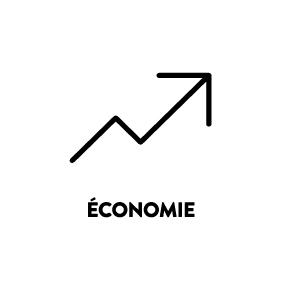
\includegraphics[width=4.85cm, height = 4.85cm]{A6_Picto_Economie}
};
% choix entre analyse défi et balises
\node[minimum width=4.5cm, minimum height = 4.5cm, draw=white, fill = orange_analyse, line width = 10pt] at (4.87,-10.17) {
};
\node[] at (4.87,-9.92) {
\color{white}\fontsize{24pt}{5pt}\selectfont Analyse
};
\node[] at (4.82,-10.52) {\color{white} \rule{3.1cm}{5pt}
};
\node[minimum width=4.5cm, minimum height = 4.5cm, draw=white, line width = 10pt] at (10.47,-10.17) {};
\node[] at (10.47,-9.87) {\calibri\color{white}\fontsize{96pt}{12pt}\selectfont \bfseries \'E};
\node[minimum width=4.5cm, minimum height = 4.5cm, draw=white, line width = 10pt] at (16.07,-10.17) {};
\node[minimum width=4.5cm, minimum height = 4.5cm, draw=white, line width = 10pt] at (4.87,-15.77) {};
\node[minimum width=4.5cm, minimum height = 4.5cm, draw=white, line width = 10pt] at (10.47,-15.77) {\calibri\color{white}\fontsize{96pt}{12pt}\selectfont\bfseries M};
\node[minimum width=4.5cm, minimum height = 4.5cm, draw=white, line width = 10pt] at (16.07,-15.77) {\calibri\color{white}\fontsize{96pt}{12pt}\selectfont\bfseries A};

% titre et sous titre et mois année à remplir
\node[minimum width=21cm, minimum height = 9cm, fill = white] at (10.5,-25.145) {
\begin{minipage}[t]{2.45cm}
\hfill
\end{minipage}\hfill
\begin{minipage}[t]{12.15cm}
\raggedright
\vspace{7.5mm}
\fontsize{20pt}{20pt}\selectfont \mdseries \titreetude\\
\helvetlight \fontsize{15pt}{15pt}\selectfont \soustitreetude \\
\color{white} \fontsize{15pt}{15pt}\selectfont \mdseries \soustitreetude \\
%\color{white} \fontsize{30pt}{30pt}\selectfont \mdseries \soustitreetude \\
\vspace{6mm}
\color{vert_n} \fontsize{10pt}{10pt}\selectfont  \bfseries \MakeUppercase{\mois~\annee} \\
\end{minipage}\hfill
\begin{minipage}[t]{6.45cm}
\hfill
\end{minipage}\hfill
};

\node[] at (10.5,-21.5) {
\begin{minipage}[t]{2.45cm}
\hfill
\end{minipage}\hfill
\begin{minipage}[t]{16.15cm}
\hfill
%{\calibri \fontsize{24pt}{12pt}\selectfont \bfseries \textls[-25]{commissariat général au développement durable}} \\
%\vspace{0.1cm}
%\hrule
\end{minipage}\hfill
\begin{minipage}[t]{2.45cm}
\hfill
\end{minipage}\hfill
};

\draw[color = black, line width = 1pt] (0,-20.65) -- (21,-20.65);
\draw[color = black, line width = 0.5pt] (0,-22) -- (21,-22);
\node[minimum width=2.95cm, minimum height = 3.8cm] at (17.10,-26) {

\includegraphics[width=2.95cm, height = 3.8cm]{Bloc-marque_MEEM_RVB_HD}
};
\end{tikzpicture}\clearpage
}

% sommaire

\newcommand\sommaire[2]{
\noindent
\begin{tikzpicture}[overlay, remember picture]
%\shade[top color=vert_n,bottom color=light_vert_n] 
%(current page.south west) rectangle (current page.north east);
\node[minimum width=21cm, minimum height = 21cm] at (10.5,-10.2) {
\includegraphics[trim = {1mm 1mm 1mm 1mm},width=21cm, height = 21cm]{fond_feuille}
};
\node[minimum width=15.65cm, minimum height = 11.15cm, draw=vert_n,fill = white, line width = 10pt] at (10.5,-12.45) {
\begin{minipage}[t]{0.62cm}
\hfill
\end{minipage}\hfill
\begin{minipage}[t]{11.70cm}
\begin{tabularx}{11cm}{clX}
\fontsize{12pt}{14pt}\selectfont \bfseries \color{vert_n} \pageref{sec:marker1} &\color{black} - & \fontsize{12pt}{12pt}\selectfont \bfseries \nameref{sec:marker1} \\
&&\\
\fontsize{12pt}{6pt}\selectfont \bfseries \color{vert_n} \pageref{sec:marker2} & \color{black} - & \fontsize{12pt}{12pt}\selectfont \bfseries \nameref{sec:marker2} \\
&&\fontsize{8pt}{9pt}\selectfont un beau résumé court \\
&&\\
\fontsize{12pt}{12pt}\selectfont \bfseries \color{vert_n} \pageref{sec:marker3} & \color{black} - & \fontsize{12pt}{12pt}\selectfont \bfseries  \nameref{sec:marker3} \\
& & \fontsize{8pt}{9pt}\selectfont A COMPLETER \\
&&\\
\fontsize{12pt}{6pt}\selectfont \bfseries \color{vert_n} \pageref{sec:marker4} & \color{black} - & \fontsize{12pt}{12pt}\selectfont \bfseries \nameref{sec:marker4}\\
&&\fontsize{8pt}{9pt}\selectfont A COMPLETER \\
&&\\
\fontsize{12pt}{6pt}\selectfont \bfseries \color{vert_n} \pageref{sec:marker5} &  \color{black} - & \fontsize{12pt}{12pt}\selectfont \bfseries \nameref{sec:marker5}\\
&&\fontsize{8pt}{9pt}\selectfont A COMPLETER \\
&&\\
\fontsize{12pt}{6pt}\selectfont \bfseries \color{vert_n} \pageref{sec:marker6} & \color{black} - & \fontsize{12pt}{12pt}\selectfont \bfseries  \nameref{sec:marker6}\\
%&&\\
%\fontsize{13pt}{13pt}\selectfont \bfseries \color{vert_n} \pageref{sec:marker7} & \normalfont \color{black} - & \nameref{sec:marker7}\\
%&&\\
%\fontsize{13pt}{13pt}\selectfont \bfseries \color{vert_n} \pageref{sec:marker8} & \normalfont \color{black} - & \nameref{sec:marker8}\\
\end{tabularx}
%\fontsize{7pt}{7pt}\selectfont
%\tableofcontents
\end{minipage}\hfill
\begin{minipage}[t]{3cm}
\hfill
\end{minipage}\hfill
};
\node[minimum width=4.5cm, minimum height = 4.5cm, draw=vert_n,fill = white, line width = 10pt] at (4.925,-4.625) {};
\node[] at (4.92,-5.55) {\centering \fontsize{16pt}{16pt} \selectfont sommaire};
\draw[line width = 5pt, color = black] (3.72,-6.0) -- (6.22,-6.0);
\node[minimum width=11.15cm, minimum height = 4.5cm, draw=vert_n,fill = white, line width = 10pt] at (12.75,-4.625) {
\begin{minipage}[t]{0.2cm}
\hfill
\end{minipage}\hfill
\begin{minipage}[t]{10.6cm}
\vspace{3mm}
\raggedright
\fontsize{20pt}{20pt}\selectfont \mdseries \titreetude \\
\helvetlight \fontsize{14pt}{20pt}\selectfont \soustitreetude \\
%\helvetlight \color{white} \fontsize{20pt}{20pt}\selectfont \soustitreetude \\
%\helvetlight \color{white} \fontsize{20pt}{20pt}\selectfont \soustitreetude \\
\end{minipage}\hfill
};
\node[minimum width=21cm, minimum height = 6.2cm, fill = white] at (10.5,-23.8) {
\begin{minipage}[t]{2.5cm}
\hfill
\end{minipage}\hfill
\begin{minipage}[t]{13cm}
\raggedright
\vspace{6mm}
{\helvetlight \fontsize{12pt}{12pt}\selectfont \textls[-10]{Document édité par :}} \\
\fontsize{12pt}{12pt}\selectfont \mdseries \textls[-10]{Le service de l'économie, de l'évaluation et} \\
\fontsize{12pt}{12pt}\selectfont \mdseries \textls[-10]{de l'intégration du développement durable (SEEIDD)} \\
%\fontsize{12pt}{12pt}\selectfont \bfseries \textls[-10]{} \\
%\fontsize{12pt}{12pt}\selectfont \bfseries \textls[-10]{} \\
%\fontsize{12pt}{12pt}\selectfont \bfseries \textls[-10]{} \\
\vspace{10mm}
\fontsize{8pt}{9pt}\selectfont \bfseries Remerciements. \fontsize{8pt}{9pt}\selectfont \normalfont  A COMPLETER \\
%\fontsize{8pt}{9pt}\selectfont \normalfont  Remerciements \\
\vspace{15.5mm}
\end{minipage}\hfill
\begin{minipage}[t]{5.5cm}
\hfill
\end{minipage}\hfill
};
\node[minimum width=21cm, minimum height = 2.5cm, fill = white] at (10.5,-28.1) {
};
\node[] at (10.5,-27.35) {
\begin{minipage}[t]{2.5cm}
\end{minipage}\hfill
\begin{minipage}[t]{16cm}
\raggedright
\textcolor{vert_n}{\rule{7pt}{7pt}} \fontsize{7}{5mm} \selectfont \thepage~ -
\textbf{\titreetude} : \soustitreetude
\end{minipage}\hfill
\begin{minipage}[t]{2.5cm}
\end{minipage}\hfill
};
\draw[color = black, line width = 0.5pt] (2.5,-26.9) -- (18.5,-26.9);
\end{tikzpicture}\clearpage 
}


% Commande pour la page contributeurs

\newcommand\contributeurs[3]{
\noindent
\begin{tikzpicture}[overlay, remember picture]
%\shade[top color=vert_n,bottom color=light_vert_n] 
%(current page.south west) rectangle (current page.north east);
\node[] at (4.12,-9.8) {\raggedright \fontsize{16pt}{7pt}\selectfont contributeurs};
\draw[line width = 5pt, color = black] (2.51,-10.21) -- (5.71,-10.21);

%contributeur 1
\node[minimum width=4.5cm, minimum height = 4.5cm, draw=vert_n,fill = white, line width = 10pt] at (10.5,-12.02) {
\begin{minipage}[t]{0.2cm}
\hfill
\end{minipage}\hfill
\begin{minipage}[t]{3.6cm}
%\vspace{2mm}
\raggedleft {\helvetlight \fontsize{42pt}{8pt}\selectfont BV}\\
\vspace{1.2cm}
\raggedright \normalfont \fontsize{11pt}{11pt}\selectfont Bruno \bfseries Vermont \\
\raggedright \fontsize{7pt}{8pt}\selectfont \bfseries Chargé d'études économiques \\
\vspace{2mm}
\raggedright \normalfont \fontsize{5pt}{6pt}\selectfont bruno.vermont@developpement-durable.gouv.fr \\
\end{minipage}
\begin{minipage}[t]{0.3cm}
\hfill
\end{minipage}\hfill
};
\node[minimum width=4.5cm, minimum height = 3.25cm] at (15,-13.64) {
\begin{minipage}[t]{0.4cm}
\hfill
\end{minipage}\hfill
\begin{minipage}[t]{3.6cm}
%\vspace{2mm}
\raggedright \fontsize{8pt}{9pt}\selectfont Chargé d'études économiques sur l'efficacité énergétique dans le secteur du bâtiment
\end{minipage}
\begin{minipage}[t]{0.3cm}
\hfill
\end{minipage}\hfill
};


%\textbf{AHOUTER SILVANO, DIMITRI?, ENERGIES DEMAIN?}

%contributeur 2
\node[minimum width=4.5cm, minimum height = 4.5cm, draw=vert_n,fill = white, line width = 10pt] at (10.5,-17.47) {
\begin{minipage}[t]{0.2cm}
\hfill
\end{minipage}\hfill
\begin{minipage}[t]{3.6cm}
%\vspace{2mm}
\raggedleft {\helvetlight \fontsize{42pt}{8pt}\selectfont SD}\\
\vspace{1.3cm}
\raggedright \fontsize{11pt}{11pt}\selectfont Silvano \bfseries Domergue \\
\raggedright \fontsize{7pt}{8pt}\selectfont \bfseries Chef de bureau \\
\vspace{2mm}
\raggedright \normalfont \fontsize{5pt}{6pt}\selectfont silvano.domergue@developpement-durable.gouv.fr \\
\end{minipage}
\begin{minipage}[t]{0.3cm}
\hfill
\end{minipage}\hfill
};
\node[minimum width=4.5cm, minimum height = 3.25cm] at (15,-18.09) {
\begin{minipage}[t]{0.4cm}
\hfill
\end{minipage}\hfill
\begin{minipage}[t]{3.6cm}
%\vspace{2mm}
\raggedright \fontsize{8pt}{9pt}\selectfont Chef du bureau économie de la transition énergétique 
\end{minipage}
\begin{minipage}[t]{0.3cm}
\hfill
\end{minipage}\hfill
};


%%contributeur 3
%\node[minimum width=4.5cm, minimum height = 4.5cm, draw=vert_n,fill = white, line width = 10pt] at (10.5,-22.92) {
%\begin{minipage}[t]{0.2cm}
%\hfill
%\end{minipage}\hfill
%\begin{minipage}[t]{3.6cm}
%%\vspace{2mm}
%\raggedleft {\helvetlight \fontsize{42pt}{8pt}\selectfont MA}\\
%\vspace{1.3cm}
%\raggedright \fontsize{11pt}{11pt}\selectfont Mobilité \bfseries Aména \\
%\raggedright \fontsize{7pt}{8pt}\selectfont \bfseries Bureau \\
%\vspace{2mm}
%\raggedright \normalfont \fontsize{5pt}{6pt}\selectfont ma@developpement-durable.gouv.fr \\
%\end{minipage}
%\begin{minipage}[t]{0.3cm}
%\hfill
%\end{minipage}\hfill
%};
%\node[minimum width=4.5cm, minimum height = 3.25cm] at (15,-23.54) {
%\begin{minipage}[t]{0.4cm}
%\hfill
%\end{minipage}\hfill
%\begin{minipage}[t]{3.6cm}
%%\vspace{2mm}
%\raggedright \fontsize{8pt}{9pt}\selectfont \bfseries Tem nam et rerro expla intem  ne audi utate \fontsize{8pt}{9pt}\selectfont \normalfont ipsunt volest eum conectaturem dolumquasi odit ut mil iurehendi aut volorro ruptaeperum event aut accum que si ipitasperia dolorem porit, omnimeTem ipsunt volestibus am, qui di conecus cientiscit laborpor molorpo rerciatem ut
%\end{minipage}
%\begin{minipage}[t]{0.3cm}
%\hfill
%\end{minipage}\hfill
%};

%pied de page
\node[] at (10.5,-27.35) {
\begin{minipage}[t]{2.5cm}
\end{minipage}\hfill
\begin{minipage}[t]{16cm}
\raggedleft
\fontsize{7}{5mm} \selectfont \textbf{\titreetude} : \soustitreetude - \thepage~  \textcolor{vert_n}{\rule{7pt}{7pt}} 
\end{minipage}\hfill
\begin{minipage}[t]{2.5cm}
\end{minipage}\hfill};
\draw[color = black, line width = 0.5pt] (2.5,-26.9) -- (18.5,-26.9);
\end{tikzpicture}
}


% Commande pour la page avant-propos

\newcommand\avantpropos[2]{
\noindent
\begin{tikzpicture}[overlay, remember picture]
%\shade[top color=vert_n,bottom color=light_vert_n] 
%(current page.south west) rectangle (current page.north east);
\node[] at (4.12,-10) {\raggedright \fontsize{16pt}{7pt}\selectfont  \textls[-5]{avant-propos} };
\draw[line width = 5pt, color = black] (2.51,-10.41) -- (5.75,-10.41);
\node[minimum width=2.99cm, minimum height = 2.99cm, draw=vert_n,fill = white, line width = 6pt] at (4.1,-12.9) {
%première lettre avant propos
\calibri\fontsize{65pt}{9pt}\selectfont \bfseries P
};
\node[minimum width=11.8cm, minimum height =  3.2cm] at (11.6,-12.9) {
\begin{minipage}[t]{0.2cm}
\hfill
\end{minipage}\hfill
\begin{minipage}[t]{11.5cm}
\helvetlight \fontsize{14pt}{17pt}\selectfont \raggedright Tem nam et rerro expla intem  ne audi utate \fontsize{8pt}{9pt}\selectfont \normalfont ipsunt volest eum conectaturem dolumquasi odit ut mil iurehendi aut volorro ruptaeperum event aut accum que si ipitasperia dolorem porit, omnimeTem ipsunt volestibus am, qui di conecus cientiscit laborpor molorpo rerciatem ut
\end{minipage}\hfill
\begin{minipage}[t]{0.1cm}
\hfill
\end{minipage}\hfill
};
\node[minimum width=16cm, minimum height = 11.2cm] at (10.5,-18) {
\begin{minipage}[t]{15cm}
\helvetlight \fontsize{14pt}{17pt}\selectfont \raggedright Tem nam et rerro expla intem  ne audi utate \fontsize{8pt}{9pt}\selectfont \normalfont ipsunt volest eum conectaturem dolumquasi odit ut mil iurehendi aut volorro ruptaeperum event aut accum que si ipitasperia dolorem porit, omnimeTem ipsunt volestibus am, qui di conecus cientiscit laborpor molorpo rerciatem ut
\end{minipage}\hfill
\begin{minipage}[t]{1cm}
\hfill
\end{minipage}\hfill
};
Tem nam et rerro expla intem  ne audi utate \fontsize{8pt}{9pt}\selectfont \normalfont ipsunt volest eum conectaturem dolumquasi odit ut mil iurehendi aut volorro ruptaeperum event aut accum que si ipitasperia dolorem porit, omnimeTem ipsunt volestibus am, qui di conecus cientiscit laborpor molorpo rerciatem ut

\node[minimum width=21cm] at (10.5,-24.78) {
\begin{minipage}[t]{2.5cm}
\hfill
\end{minipage}\hfill
\begin{minipage}[t]{12cm}
\raggedright \fontsize{13pt}{20pt}\selectfont Laurence Monnoyer-Smith \\
\helvetlight \fontsize{9pt}{9pt}\selectfont \textls[10]{COMMISSAIRE G\'{E}N\'{E}RALE AU D\'{E}VELOPPEMENT DURABLE} \hfill
\end{minipage}
\begin{minipage}[t]{4cm}
\hfill
%\includegraphics[width=5cm, height = 3cm]{signature}
\end{minipage}\hfill
\begin{minipage}[t]{2.5cm}
\hfill
\end{minipage}\hfill};

%
%\node[minimum width=12.5cm] at (14.75,-24.78) {
%\begin{minipage}[t]{4cm}
%\hfill
%%SIGNATURE 
%\end{minipage}\hfill
%\begin{minipage}[t]{2.5cm}
%\hfill
%\end{minipage}\hfill};

\node[] at (10.5,-27.35) {
\begin{minipage}[t]{2.5cm}
\end{minipage}\hfill
\begin{minipage}[t]{16cm}
\raggedright
\textcolor{vert_n}{\rule{7pt}{7pt}} \fontsize{7}{5mm} \selectfont \thepage~ -
\textbf{\titreetude} : \soustitreetude
\end{minipage}\hfill
\begin{minipage}[t]{2.5cm}
\end{minipage}\hfill
};
\draw[color = black, line width = 0.5pt] (2.5,-26.9) -- (18.5,-26.9);
\end{tikzpicture}
}


% Commande pour la troisième de couv

\newcommand\troisieme[2]{
\noindent
\begin{tikzpicture}[overlay, remember picture]
%\shade[top color=vert_n,bottom color=light_vert_n] 
%(current page.south west) rectangle (current page.north east);
\node[minimum width=21cm, minimum height = 21cm] at (10.5,-10.2) {
\includegraphics[trim = {1mm 1mm 1mm 1mm},width=21cm, height = 21cm]{fond_feuille2}
};
\node[minimum width=21cm, minimum height = 9cm, fill = white] at (10.5,-25.145) {};

\node[minimum width=21cm, minimum height = 4.5cm] at (10.5,-22.4) {
\begin{minipage}[t]{2.5cm}
\hfill
\end{minipage}\hfill
\begin{minipage}[t]{11.9cm}
\fontsize{8pt}{7.8pt}\selectfont \bfseries
Conditions générales d’utilisation\\
\fontsize{6.5pt}{7.8pt}\selectfont \normalfont 
\raggedright
Toute reproduction ou représentation intégrale ou partielle, par quelque procédé que ce soit, des pages publiées
dans le présent ouvrage, faite sans l’autorisation de l’éditeur ou du Centre français d’exploitation du droit de copie
(3, rue Hautefeuille — 75006 Paris), est illicite et constitue une contrefaçon. Seules sont autorisées, d’une part,
les reproductions strictement réservées à l’usage privé du copiste et non destinées à une utilisation collective, et,
d’autre part, les analyses et courtes citations justifiées par le caractère scientifque ou d’information de l’oeuvre
dans laquelle elles sont incorporées (loi du 1er juillet 1992 — art. L.122-4 et L.122-5 et Code pénal art. 425).
\end{minipage}\hfill
\begin{minipage}[t]{6.5cm}
\hfill
\end{minipage}\hfill
};

\node[minimum width=21cm, minimum height = 4.5cm] at (10.5,-25) {
\begin{minipage}[t]{2.5cm}
\hfill
\end{minipage}\hfill
\begin{minipage}[t]{3.5cm}
\fontsize{8pt}{9.6pt}\selectfont \bfseries \raggedright
\bfseries  Dépôt légal : \normalfont Octobre 2016 \\
\bfseries  ISSN : \normalfont En cours \\
%\bfseries  ISBN : \normalfont XXX-X-XX-XXXXXX-X
\end{minipage}\hfill
\begin{minipage}[t]{0.8cm}
\hfill
\end{minipage}\hfill
\begin{minipage}[t]{7.5cm}
\fontsize{8pt}{9.6pt}\selectfont \color{white} \raggedright
Achevé d'imprimer en mois XXXX.\\
\bfseries Impression : \normalfont Lieu, utilisant du papier\\
issu de forêts durablement gérées.\\
\end{minipage}\hfill
\begin{minipage}[t]{6.5cm}
\hfill
\end{minipage}\hfill
};

%pied de page
\node[] at (10.5,-27.35) {
\begin{minipage}[t]{2.5cm}
\end{minipage}\hfill
\begin{minipage}[t]{16cm}
\raggedleft
\fontsize{7}{5mm} \selectfont \textbf{\titreetude} : \soustitreetude - \thepage~  \textcolor{vert_n}{\rule{7pt}{7pt}} 
\end{minipage}\hfill
\begin{minipage}[t]{2.5cm}
\end{minipage}\hfill};
\draw[color = black, line width = 0.5pt] (2.5,-26.9) -- (18.5,-26.9);


\end{tikzpicture}
}

%Commande pour la quatrième de couv
\newcommand\quatrieme[1]{
\noindent
\begin{tikzpicture}[overlay, remember picture]
%\shade[top color=vert_n,bottom color=light_vert_n] 
%(current page.south west) rectangle (current page.north east);
\node[minimum width=21cm, minimum height = 21cm] at (10.5,-10.2) {
\includegraphics[trim = {1mm 1mm 1mm 1mm},width=21cm, height = 21cm]{fond_feuille2}
};

\node[minimum width=4.5cm, minimum height = 4.5cm, draw=white, line width = 10pt] at (4.87,-4.57) {};

\node[minimum width=4.5cm, minimum height = 4.5cm, draw=white, line width = 10pt] at (4.87,-10.17) {
};
\node[minimum width=4.5cm, minimum height = 4.5cm, draw=white,fill = white,, line width = 10pt] at (4.87,-15.77) {\begin{minipage}{0.3cm}
\hfill
\end{minipage}\hfill
\begin{minipage}{3.6cm}
\raggedright
\mdseries \color{vert_n}\fontsize{16pt}{16pt}\selectfont \titreetude  \\
\helvetlight \color{vert_n}\fontsize{16pt}{16pt}\selectfont \soustitreetude
\vspace{2cm}
\end{minipage}\hfill
\begin{minipage}{0.3cm}
\hfill
\end{minipage}\hfill};
\node[minimum width=4.5cm, minimum height = 4.5cm, draw=white, line width = 10pt] at (10.47,-15.77) {
};
\node[minimum width=4.5cm, minimum height = 4.5cm, draw=white, line width = 10pt] at (16.07,-15.77) {};

\node[minimum width=10.1cm, minimum height = 10.1cm, draw=white, fill = white, line width = 10pt] at (13.27,-7.37) {
\begin{minipage}[t]{0.2cm}
\hfill
\end{minipage}\hfill
\begin{minipage}[t]{9.25cm}
\vspace{2mm}
{\helvetlight \fontsize{10pt}{11pt}\selectfont #1 \hfill}
\end{minipage}\hfill
\begin{minipage}[t]{0.2cm}
\hfill
\end{minipage}\hfill
};


\node[minimum width=21cm, minimum height = 9cm, fill = white] at (10.5,-25.145) {
\begin{minipage}[t]{2.45cm}
\hfill
\end{minipage}\hfill
\begin{minipage}[t]{16.15cm}
\raggedright
\vspace{5mm}
\helvetlight \fontsize{12pt}{13pt} \selectfont Service de l'économie, de l'évaluation et de l'intégration du développement durable \\
Sous-direction mobilité et aménagement \\
Tour Sequoia \\
92055 La Défense cedex \\
courriel : ma.seei.cgdd@developpement-durable.gouv.fr
\vspace{3.5cm}
\end{minipage}\hfill
\begin{minipage}[t]{2.45cm}
\hfill
\end{minipage}\hfill
}
;


\node[] at (10.5,-21.5) {
\begin{minipage}[t]{2.45cm}
\hfill
\end{minipage}\hfill
\begin{minipage}[t]{16.15cm}
{\calibri \fontsize{24pt}{12pt}\selectfont \bfseries \textls[-25]{commissariat général au développement durable}} \\
%\vspace{0.1cm}
%\hrule
\end{minipage}\hfill
\begin{minipage}[t]{2.45cm}
\hfill
\end{minipage}\hfill
};
\draw[color = black, line width = 1.5pt] (0,-20.6) -- (21,-20.6);
\draw[color = black, line width = 0.5pt] (0,-22) -- (21,-22);
\node[minimum width=2.95cm, minimum height = 3.8cm] at (17.10,-26) {

\includegraphics[width=2.95cm, height = 3.8cm]{Bloc-marque_MEEM_RVB_HD}
};

\node[minimum width=21cm, minimum height = 2cm] at (10.5,-27.7) {
\begin{minipage}[t]{2.45cm}
\hfill
\end{minipage}\hfill
\begin{minipage}[t]{16.15cm}
 \fontsize{10pt}{10pt}\selectfont \bfseries www.developpement-durable.gouv.fr
\end{minipage}\hfill
\begin{minipage}[t]{2.45cm}
\hfill
\end{minipage}\hfill
};
\end{tikzpicture}
}
% couleurs et polices des sections
\usepackage{sectsty}
\usepackage[noindentafter]{titlesec}
\renewcommand\thesection{\arabic{section}}
\titleformat{\section}{\raggedright \sloppy}{}{0em}{\fontsize{35}{36}\selectfont}
\titlespacing*{\section}{0mm}{0mm}{9mm}


% titre de section invisible
\makeatletter
\newcommand\invisiblesection[1]{%
  \refstepcounter{section}%
  \def\@currentlabelname{#1}
  \addcontentsline{toc}{section}{\protect\numberline{\thesection}#1}%
  \sectionmark{#1}}
\makeatother


% version officielle
%\titleformat{\subsection}{\raggedright \sloppy}{}{0em}{\fontsize{35}{36}\selectfont}
%\titlespacing*{\subsection}{0mm}{0mm}{12mm}
%\titleformat{\subsubsection}{\color{vert_n}\bfseries}{}{0em}{\fontsize{10.5}{12}\selectfont \scshape \uppercase}
%\titleformat{\subsubsubsection}{\bfseries\fontsize{10.5}{12}\selectfont}{\thesubsubsection}{1em}{}
%\titlespacing*{\subsubsubsection}{ 0mm }{7.5mm}{ 0mm }

% version décalée d'un niveau
%\titleformat{\subsection}{\raggedright \sloppy}{}{0em}{\fontsize{35}{36}\selectfont}
%\titlespacing*{\subsection}{0mm}{0mm}{12mm}
\titleformat{\subsection}{\color{vert_n}\bfseries}{}{0em}{\fontsize{10.5}{12}\selectfont \scshape \uppercase}
\titleformat{\subsubsection}{\bfseries\fontsize{10.5}{12}\selectfont}{\thesubsubsection}{1em}{}
\titlespacing*{\subsubsection}{0mm}{0mm}{ 0mm }


% marges
\usepackage[%
      headheight=2.85cm,
			headsep = 1.85cm,
      includeheadfoot,
      margin=2.5cm,
			marginparsep = 0cm, 
      textheight=19.25cm, 
		%	showframe, 
			footskip = 17mm,
			includehead, includefoot,
			left=2.5cm,right=2.5cm,
			top=2.5cm,bottom=2.5cm,
			asymmetric,
]{geometry}

\setlength{\oddsidemargin}{0cm}
\setlength{\evensidemargin}{0cm}


%\setlength{\voffset}{-0.04cm}
%\setlength{\hoffset}{0cm}
%\setlength{\footskip}{17mm}

% en tête et pied de page
\usepackage{fancyhdr}
% nouvelle commande hrule avec un paramètre pour définir l'écart avant ou après
\newcommand{\HRule}[1][\medskipamount]{\par
  \vspace*{\dimexpr-\parskip-\baselineskip+#1}
  \noindent\rule{\linewidth}{10pt}\par
  \vspace*{\dimexpr-\parskip-.5\baselineskip+#1}}
	

\fancyhead{}
\renewcommand{\headrulewidth}{0.5pt}
\fancyhead{} 
\fancyhead[L]{
\textcolor{vert_n}{\HRule[0pt]}
\vspace{0.2cm}
\setlength{\fboxsep}{0mm}
\fcolorbox{white}{white}{\parbox[t][2.3cm]{7.8cm}{\fontsize{10pt}{10pt} \selectfont \textls[-10]{\nouppercase{\leftmark}}}}
}

\fancyfoot{}
\renewcommand{\footrulewidth}{0.5pt}
\fancyfoot[LE]{ \textcolor{vert_n}{\rule{7pt}{7pt}} \fontsize{7}{5mm} \selectfont \thepage~ -
\textbf{\titreetude} - \soustitreetude}
 \fancyfoot[RO]{\fontsize{7pt}{5mm} \selectfont \textbf{\titreetude} - \soustitreetude - \thepage~  \textcolor{vert_n}{\rule{7pt}{7pt}}}


% page style première page partie
\fancypagestyle{partie}{%
\newgeometry{headheight=0cm,
			headsep = 0cm,
      margin=0cm,
			marginparsep = 0cm, 
      textheight=0cm, 
	%		showframe, 
			footskip = 0mm,
			includehead, includefoot,
			left=0cm,right=0cm,
			top=0cm,bottom=0cm,asymmetric}
\fancyhf{} % clear all header and footer fields
\renewcommand{\headrulewidth}{0pt}
\renewcommand{\footrulewidth}{0pt}
}

%##################################################################
%######## Langue et sommaire
%##################################################################

\usepackage[frenchb]{babel}
\usepackage{enumitem}

%indentation des paragraphes (garder l'odre !!)
\setlength{\parindent}{5mm}
\frenchbsetup{IndentFirst=false}
%\frenchbsetup{StandardLists=true}
\selectlanguage{frenchb} 
% espaces entre les paragraphes 
\setlength{\parskip}{3mm}

\usepackage{caption}
\setcounter{tocdepth}{2}
\setcounter{secnumdepth}{1}
%couleurs et polices des titres de figures 
\captionsetup[figure]{labelfont={bf},textfont={small,bf}}
\captionsetup[table]{labelfont={bf},textfont={small,bf}, name = Tableau}

\addtocontents{toc}{\protect\thispagestyle{fancy}}

%change le nom de la table des matières+couleurs
\addto\captionsfrench{% Replace "english" with the language you use
 \renewcommand{\contentsname}%
 {}%
}

%change le nom de la table des matières+couleurs
\addto\captionsfrench{% Replace "english" with the language you use
 \renewcommand{\contentsname}%
 {}%
}

%Définit le titre et le sous-titre A modifier
\newcommand\titreetude{Scénarios de rénovation énergétique des bâtiments tertiaire}
\newcommand\soustitreetude{Quelles solutions pour quels coûts à l'horizon 2050 ?}
\newcommand\annee{2019}
\newcommand\mois{MARS}

\AtBeginDocument{\addtocontents{toc}{\protect\thispagestyle{partie}}} 
\begin{document}

\pagestyle{fancy}

%\end{titlepage}

\thispagestyle{partie}
\pagetitre{}{}{}{}

\newpage 

\thispagestyle{partie}
\sommaire{}{}

\newpage 

\thispagestyle{partie}
\contributeurs{}{}

\newpage 

\thispagestyle{partie}
\avantpropos{}{}

\cleardoublepage
%\thispagestyle{partie}
%\cadreblanc{}{Introduction}

\newpage
\pagestyle{fancy}

{\fontsize{10.5pt}{12pt}\selectfont 

%\invisiblesection{Introduction}\label{sec:marker1}
\section{Introduction}\label{sec:marker1}

\markboth{Introduction}{}

%\begin{itemize}

\subsection{La part du secteur tertiaire dans les consommations et les émissions de GES en France}

\subsection{les objectifs des politiques publiques impactant le tertiaire}

\subsection{Littérature sur le sujet de la rénovation dans le tertiaire??}

\subsection{Apports et structure de l'étude}




\cleardoublepage

\thispagestyle{partie}
\cadreblanc{Partie 1}{État initial du parc tertiaire }{Résumé Partie}

\newpage
\pagestyle{fancy}

\invisiblesection{État initial du parc tertiaire}\label{sec:marker2}
\markboth{Partie 1 : État initial du parc tertiaire}{}

Le point de départ de la construction d'un modèle dynamique d'évolution du parc tertiaire est la définition d’un état initial détaillé qui sert de base à la mise en dynamique du parc de l’année de référence 2009 à l’horizon 2050. L’état des lieux a été déterminé avec le modèle ENERTER Tertiaire, développé par Energies Demain.

\subsection{Reconstitution statistique des surfaces du parc tertiaire}

Energies Demain et le Centre Energétique et Procédés (CEP) de l’Ecole des Mines de Paris ont conjointement travaillé au développement d’une méthodologie de reconstitution du parc tertiaire dans le cadre de l'élaboration du modèle ENERTER Tertiaire qui se décline en deux étapes : 

\begin{itemize}
	\item La description du parc qui consiste en une caractérisation aussi bien quantitative que qualitative du parc bâti tertiaire
	\item L’évaluation des consommations d’énergie du parc tertiaire à l’aide d’un moteur de calcul dynamique
\end{itemize}

Les surfaces chauffées ont été reconstituées pour les huit branches d’activité tertiaire selon la définition du Centre d’Études et de Recherches Économiques sur l’Énergie (CEREN) : Bureaux Administration, Café Hôtel Restaurant, Commerce, Enseignement Recherche, Habitat Communautaire, Santé Action Sociale, Sport Loisir Culture et Équipements Collectifs Divers, Transport. 

La quantification des surfaces est effectuée à partir de données sur l’emploi actuel ainsi que l’activité, le nombre et la taille des établissements implantés dans chacune des communes françaises. Les données utilisées sont celles du dénombrement des établissements de l’INSEE, l’historique des recensements généraux de la population, les données de l’emploi des bases SIRENE et UNISTATIS, ainsi que des bases de données spécifiques à la branche étudiée. 

A titre illustratif, dans le cas de la branche « Habitat Communautaire », comprenant notamment les maisons de retraite, la Base Permanente des Équipements de l’INSEE, les données du Fichier National des Etablissements Sanitaires et Sociaux (FINESS) ainsi que celles des Statistiques Annuelles des Établissements de Santé (SAE) sont venues compléter l’approche statistique basée sur l’emploi salarié par des données territorialisées renseignant le nombre de lits, de pensionnaires ainsi que d’établissements selon la nature de l’activité exercée et la période de construction.

Ceci permet d’obtenir une répartition des surfaces chauffées, des salariés et des unités d’occupant (élèves, chambres, lits…) à l’échelle de l’établissement selon les discriminants suivants :
\begin{itemize}
\item	Activité détaillée (selon le code NAF rev.1 2003 ou rev.2 2008)
\item	Secteur (Public/Privé/Parapublic)
\item	Statut juridique (Etablissement public administratif, Association loi 1901, SARL, Fondation…)
\item	Occupant (Etat, Régions, Départements, Bloc communal, Parapublic, Privé)
\end{itemize}


\cadrevert{Les sources de données utilisées}{
\vspace{0.2cm}
{\centering\fontsize{7}{8}\selectfont
\begin{tabular}{l|l}
\textbf{Branche d'activité}	&	\textbf{Source de données}
\\	\hline	\\	
						&	Emploi départemental base UNISTATIS  \\
						&	Recensements de la population version longue (INSEE) \\
Bureaux Administration	& 	Dénombrement des établissements 2008 (INSEE) \\
						&	Base permanente des équipements 2008 (INSEE) \\
						&	Bureaux, ADEME AICVF \\
						&	Rapport du projet Optisol, ADEME/ARMINES, 2009\\
\\	\hline	\\				
						&	Dénombrement des établissements 2008 (INSEE) \\
						&	Base permanente des équipements 2008 (INSEE) \\
Café Hôtel Restaurant	& 	Capacité des communes en hébergement touristique (INSEE), 2010 \\
						&	Hôtels Restaurants, ADEME AICVF \\
						&	Rapport du projet Optisol, ADEME/ARMINES, 2009 \\
\\	\hline	\\
						&	Dénombrement des établissements 2008 (INSEE) \\
						&	Base permanente des équipements 2008 (INSEE) \\
Commerce				& 	Atlas de la distribution, LSA, 2011 \\
						&	Les points de vente en 2004, INSEE \\
						&	Rapport du projet Optisol, ADEME/ARMINES, 2009 \\
\\	\hline	\\					
						&	Dénombrement des établissements 2008 (INSEE) \\
						&	Base permanente des équipements 2008 (INSEE) \\
Enseignement Recherche	& 	Repères et références statistiques 2009 (MEN) \\
						&	Atlas régional de l’enseignement supérieur 2008 (MESR) \\
						&	Rapport du projet Optisol, ADEME/ARMINES, 2009 \\
\\	\hline	\\
						&	Dénombrement des établissements 2008 (INSEE) \\
						&	Base permanente des équipements 2008 (INSEE) \\
Habitat Communautaire	& 	Fichier National des Etablissements Sanitaires et Sociaux (FINESS) \\
						&	Rapport du projet Optisol, ADEME/ARMINES, 2009 \\
\\	\hline	\\
						&	Dénombrement des établissements 2008 (INSEE) \\
						&	Base permanente des équipements 2008 (INSEE) \\
Santé Action Sociale	& 	Fichier National des Etablissements Sanitaires et Sociaux (FINESS) \\
						&	Base de Statistique Annuelle des Etablissements de santé (SAE) \\
						&	Rapport du projet Optisol, ADEME/ARMINES, 2009 \\
\\	\hline	\\
						&	Dénombrement des établissements 2008 (INSEE) \\
Sport Loisir Culture	&	Base permanente des équipements 2008 (INSEE), théâtres et cinémas \\
et équipements collectifs 	& 	Recensement des équipements sportifs \\
divers					&	Sports, ADEME AICVF \\
						&	Rapport du projet Optisol, ADEME/ARMINES, 2009 \\
\\	\hline	\\
Transport				&	Dénombrement des établissements 2008 (INSEE)
\end{tabular}
}
}

Les surfaces obtenues sont calées sur la base de données de cadrage disponibles aux échelles régionale et nationale. Les surfaces par branche d'activité sont notamment calées pour correspondre aux surfaces des données de parc du CEREN à l'échelle nationale (figure~\ref{CompParcCEREN2010}). La surface totale de parc est de 922 Mm2 à l’état initial dans le modèle (en 2010), la répartition du parc tertiaire par branche d’activité est diversifié. Elle est dominé par les activités de bureaux, de commerce, et d’enseignement/recherche, qui constituent à eux trois presque les deux tiers du parc.

\begin{figure}[ht]
\centering
\caption{Comparaison du parc initial du modèle par branche avec les données de parc du CEREN (2010)}\label{CompParcCEREN2010}
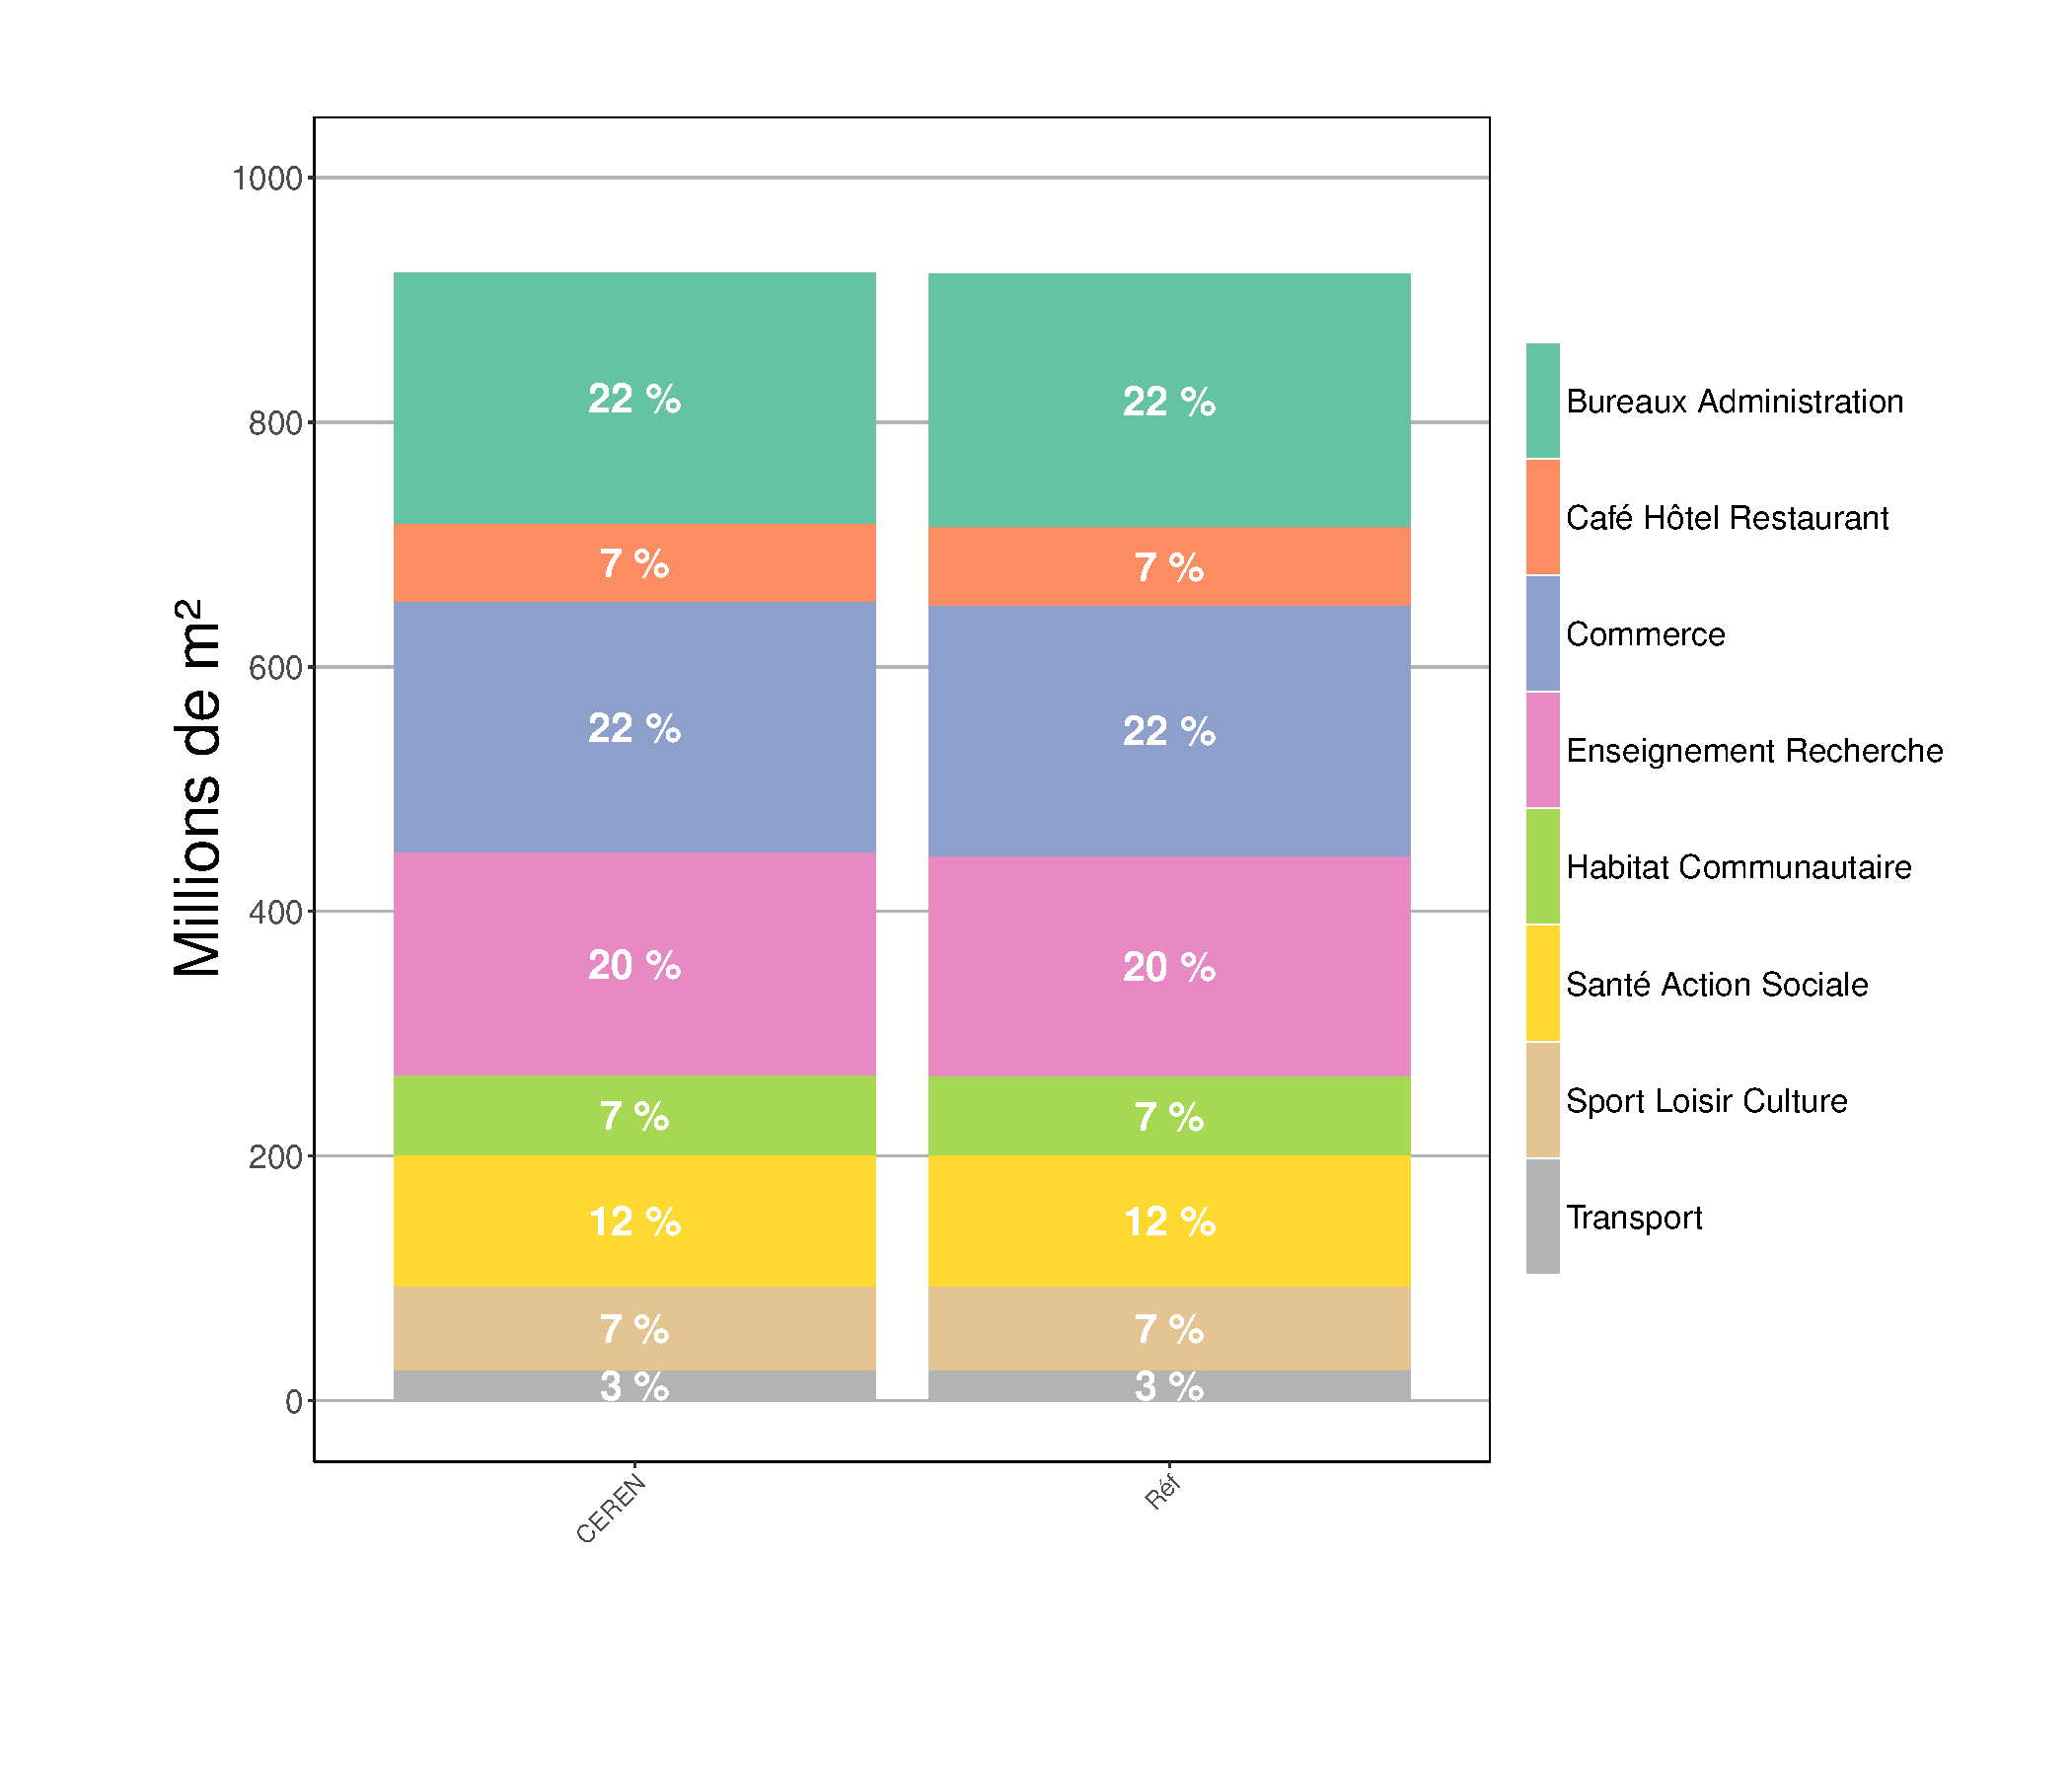
\includegraphics[width = 0.8\textwidth]{CompParcCEREN2010}
\end{figure}

Le parc peut également être catégorisé par période de construction. Les bâtiments tertiaires ont été majoritairement construits avant 1980 (56~\%),  26~\% ont été construits entre 1980 et 1998, et 18~\% des bâtiments ont moins de 20 ans. Cette distribution par période de construction est relativement similaire si on l'observe par branche d'activité avec néanmoins quelques particularités pour les branches \og Café Hôtel Restaurant \fg~et  \og Transport \fg~dont les bâtiments sont plus anciens (figure \ref{ParcPeriode2010}). 

\begin{figure}[ht]
\centering
\caption{Période de construction des bâtiments par branche d'activité en 2010}\label{ParcPeriode2010}
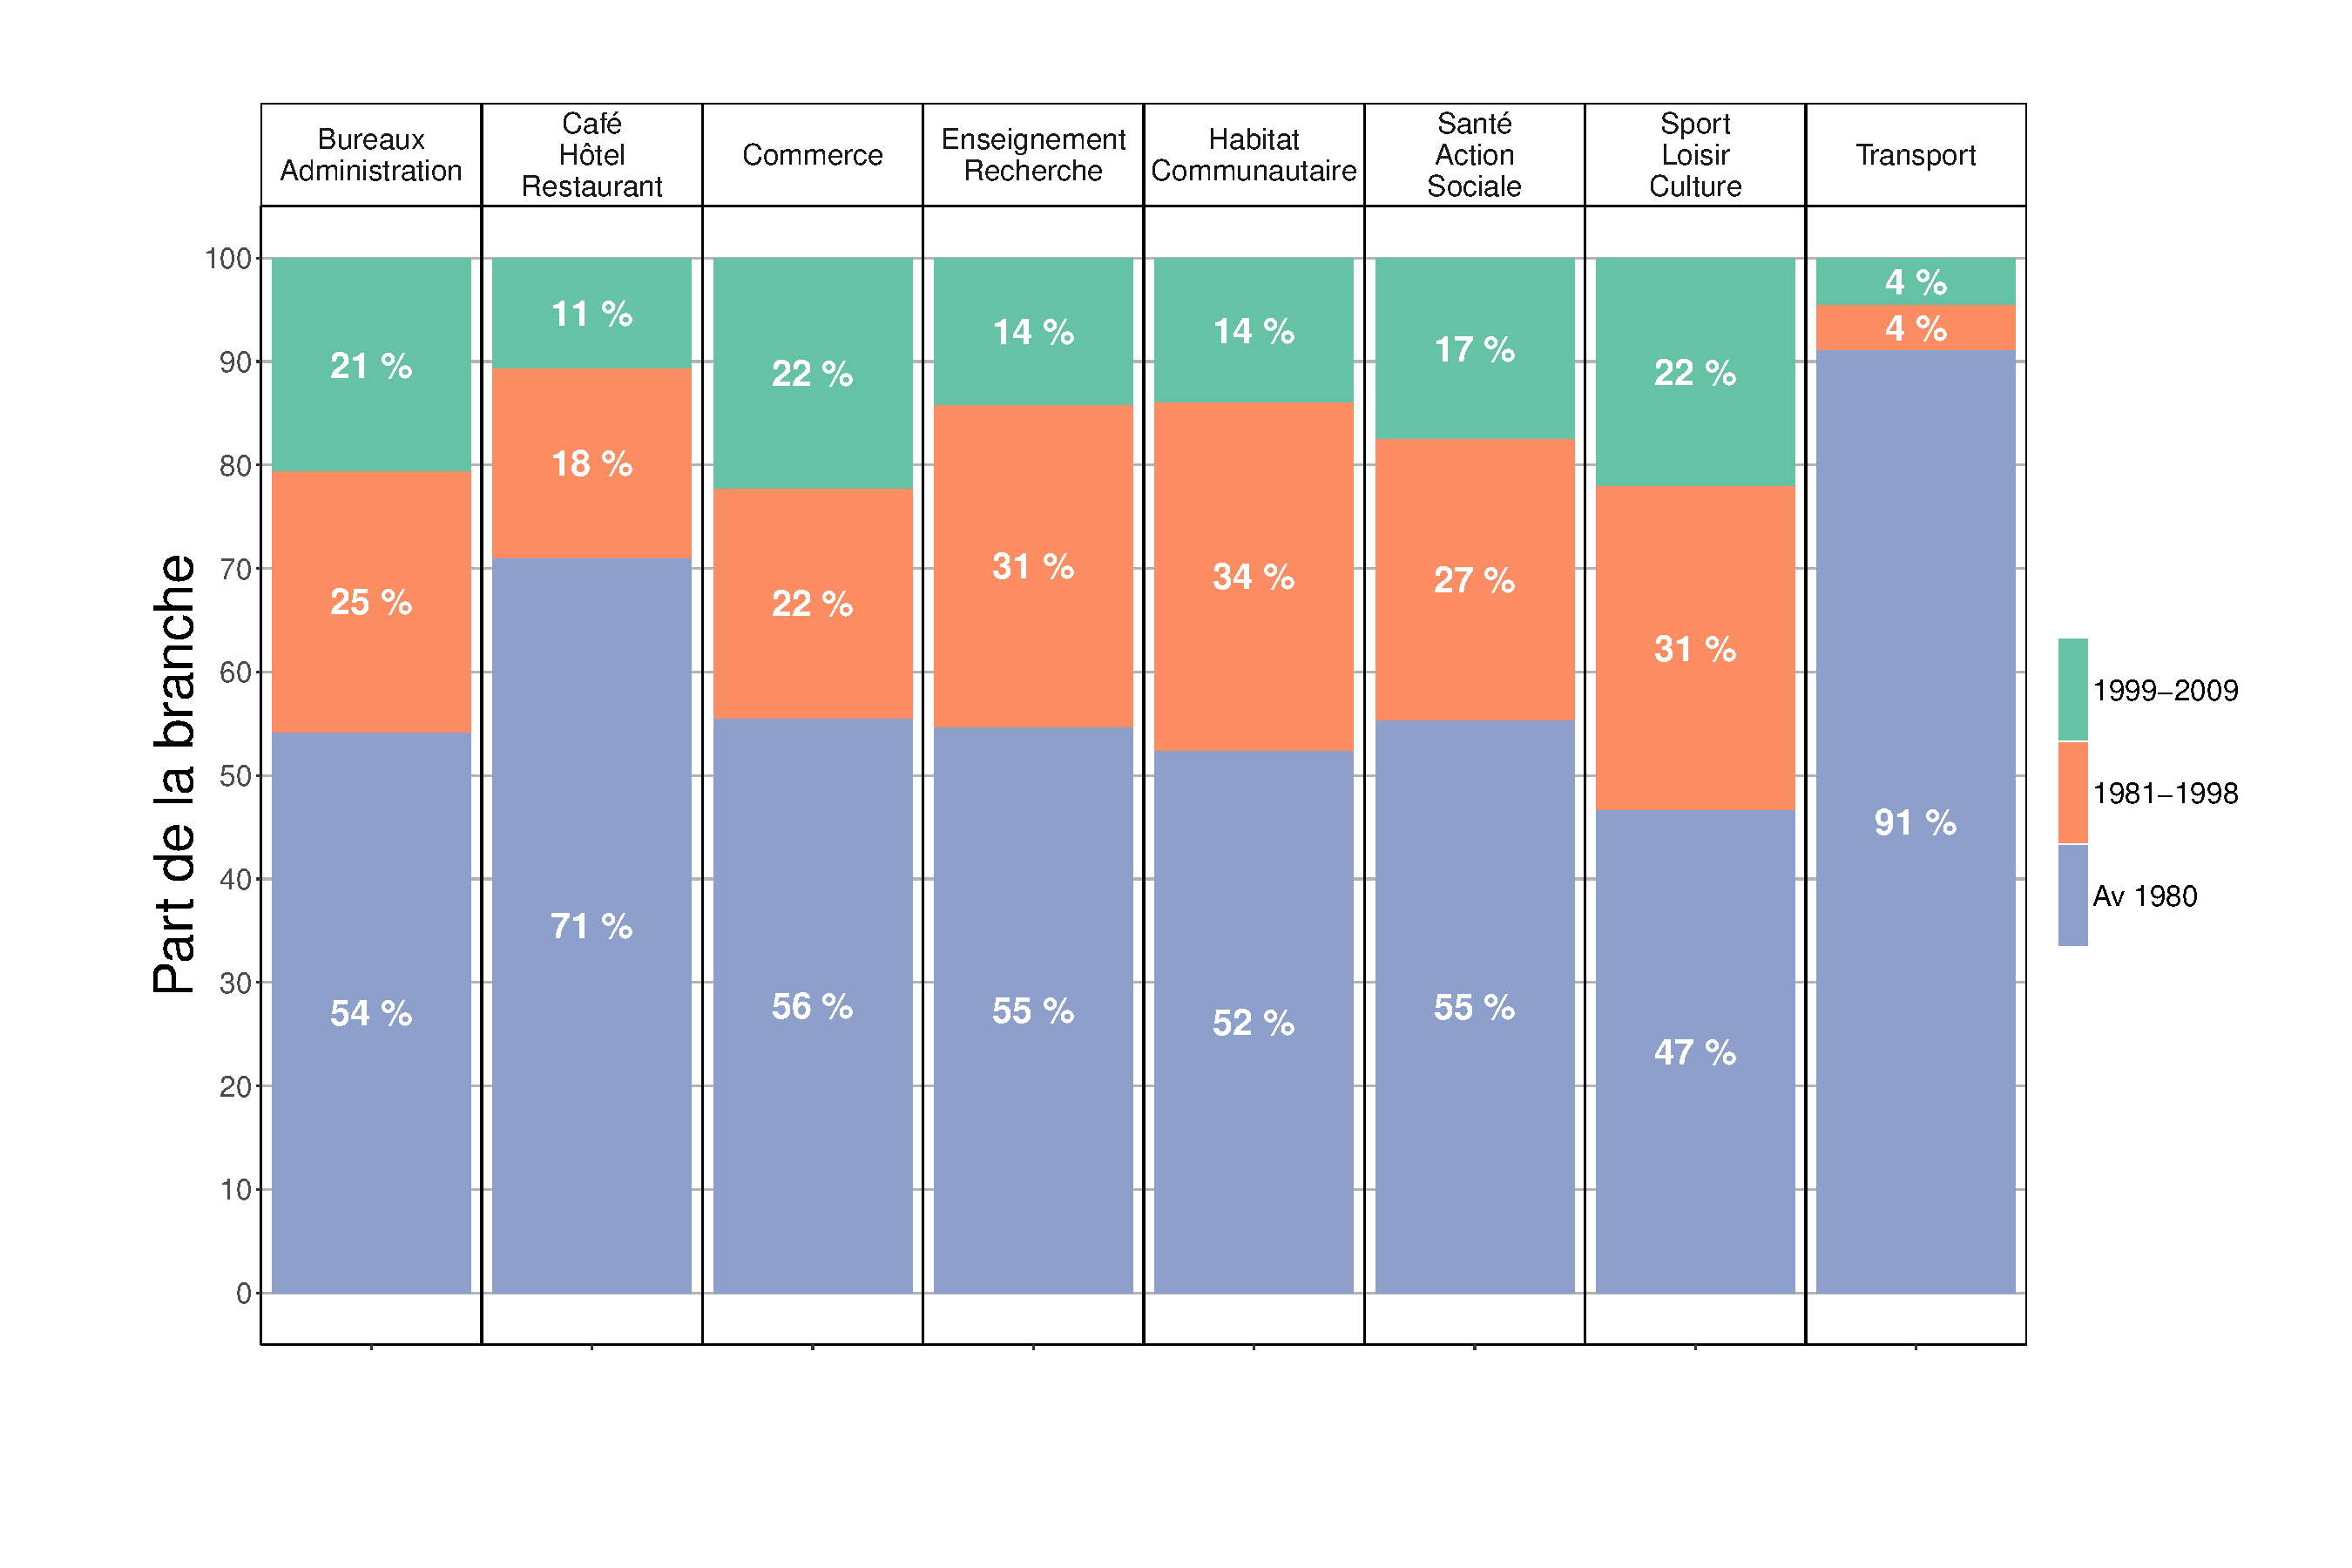
\includegraphics[width = 0.8\textwidth]{ParcPeriodeBranche2010}
\end{figure}

\subsection{Parts de marchés des énergies}

Les parts de marché des énergies selon leur usage sont déterminées en fonction des statistiques énergétiques existantes à l’échelle régionale, ainsi que selon la disponibilité des énergies à l’échelle communale (ex : présence ou non d’un réseau de chaleur ou du gaz en réseau). Les surfaces par énergie de chauffage à l'échelle nationale sont calées pour correspondre aux surfaces totales par énergie du CEREN en 2010 (figure \ref{CompParcEnergieCEREN2010}). 

Cinq énergies de chauffage sont retenues dans le cadre du modèle : Electricité, Gaz de réseau, Fioul, Réseau de chauffage urbain, Autres. L’énergie « Autres » est constituée du GPL, de la biomasse, de l’énergie solaire et du charbon, dans des proportions non connues faute de données précises disponibles. En 2010, le parc tertiaire est majoritairement chauffé au gaz (46~\%). Il existe des disparités dans les parts de marché des énergie entre les branches d'activité : les branches \og Bureaux Administration \fg~, \og Café Hôtel Restaurant \fg~ et \og Commerce \fg~ présentent par exemple une part de l'électricité plus importante que la moyenne (figure \ref{ParcEnergieBranche2010}). 


\begin{figure}[ht]
\centering
\caption{Comparaison du parc initial du modèle par énergie avec les données de parc du CEREN (2010)}\label{CompParcEnergieCEREN2010}
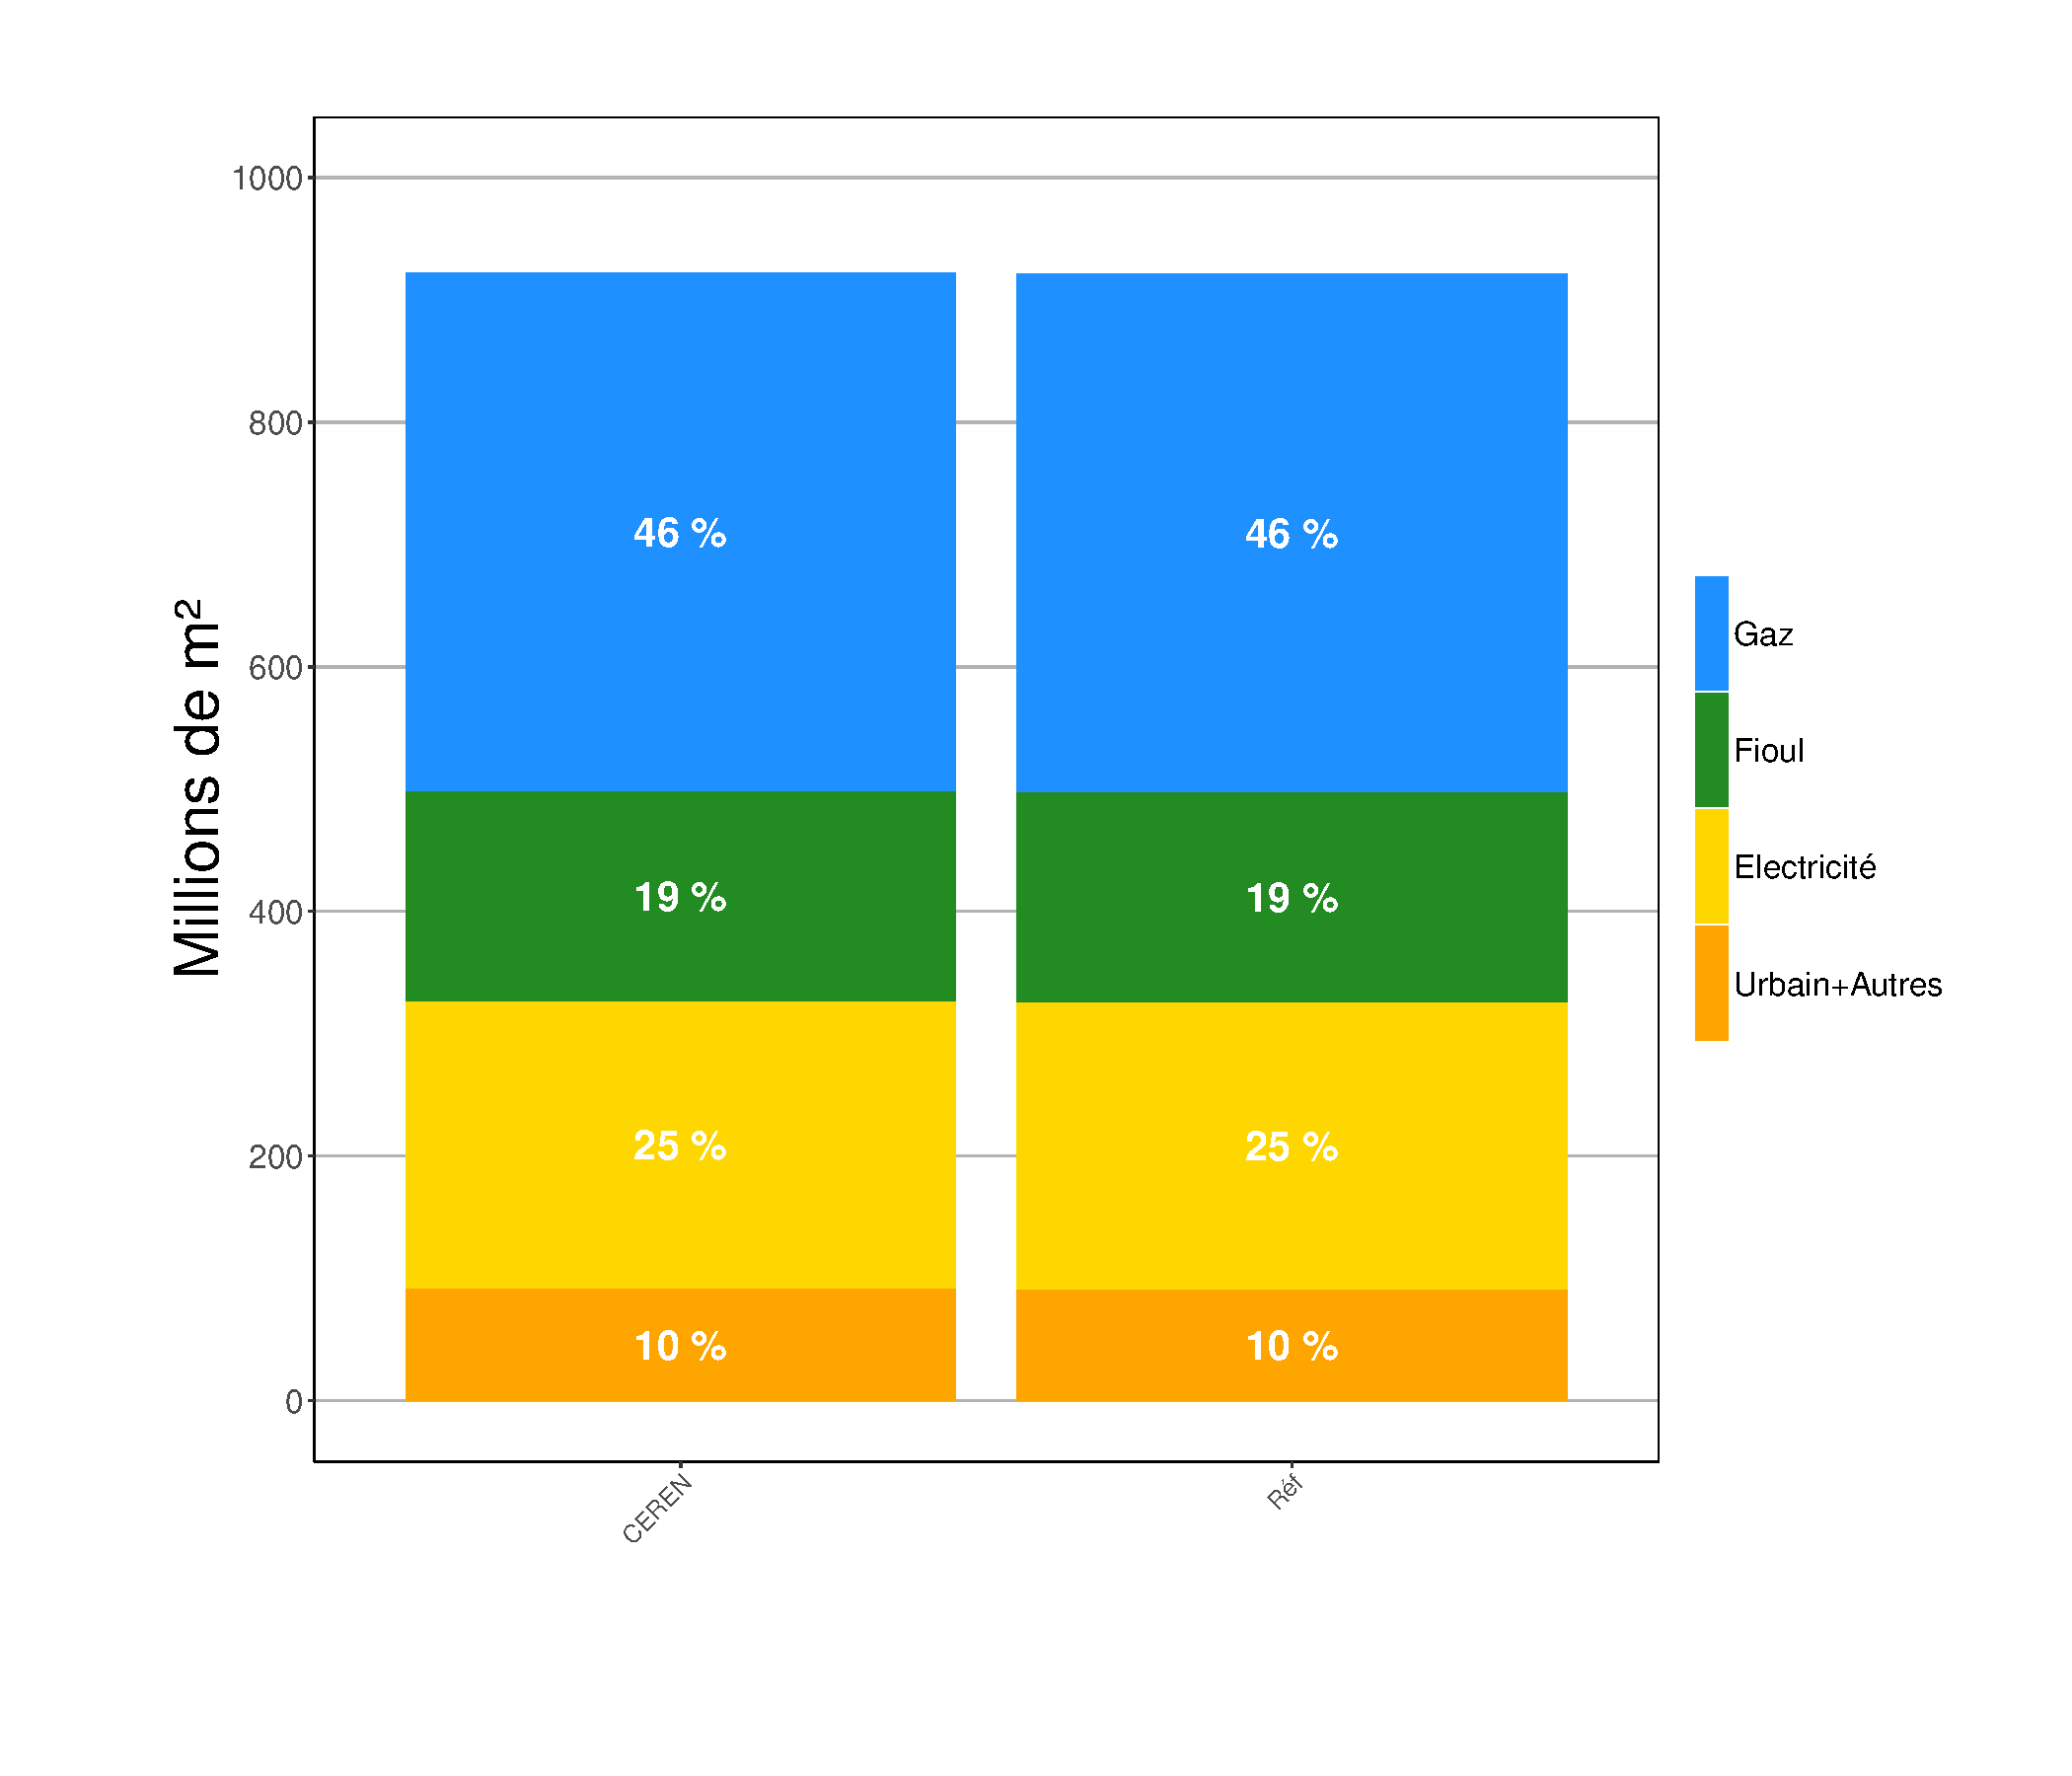
\includegraphics[width = 0.7\textwidth]{CompParcEnergieCEREN2010}
\end{figure}


\begin{figure}[ht]
\centering
\caption{Parts de marchés surfaciques des énergies par branche d'activité en 2010  }\label{ParcEnergieBranche2010}
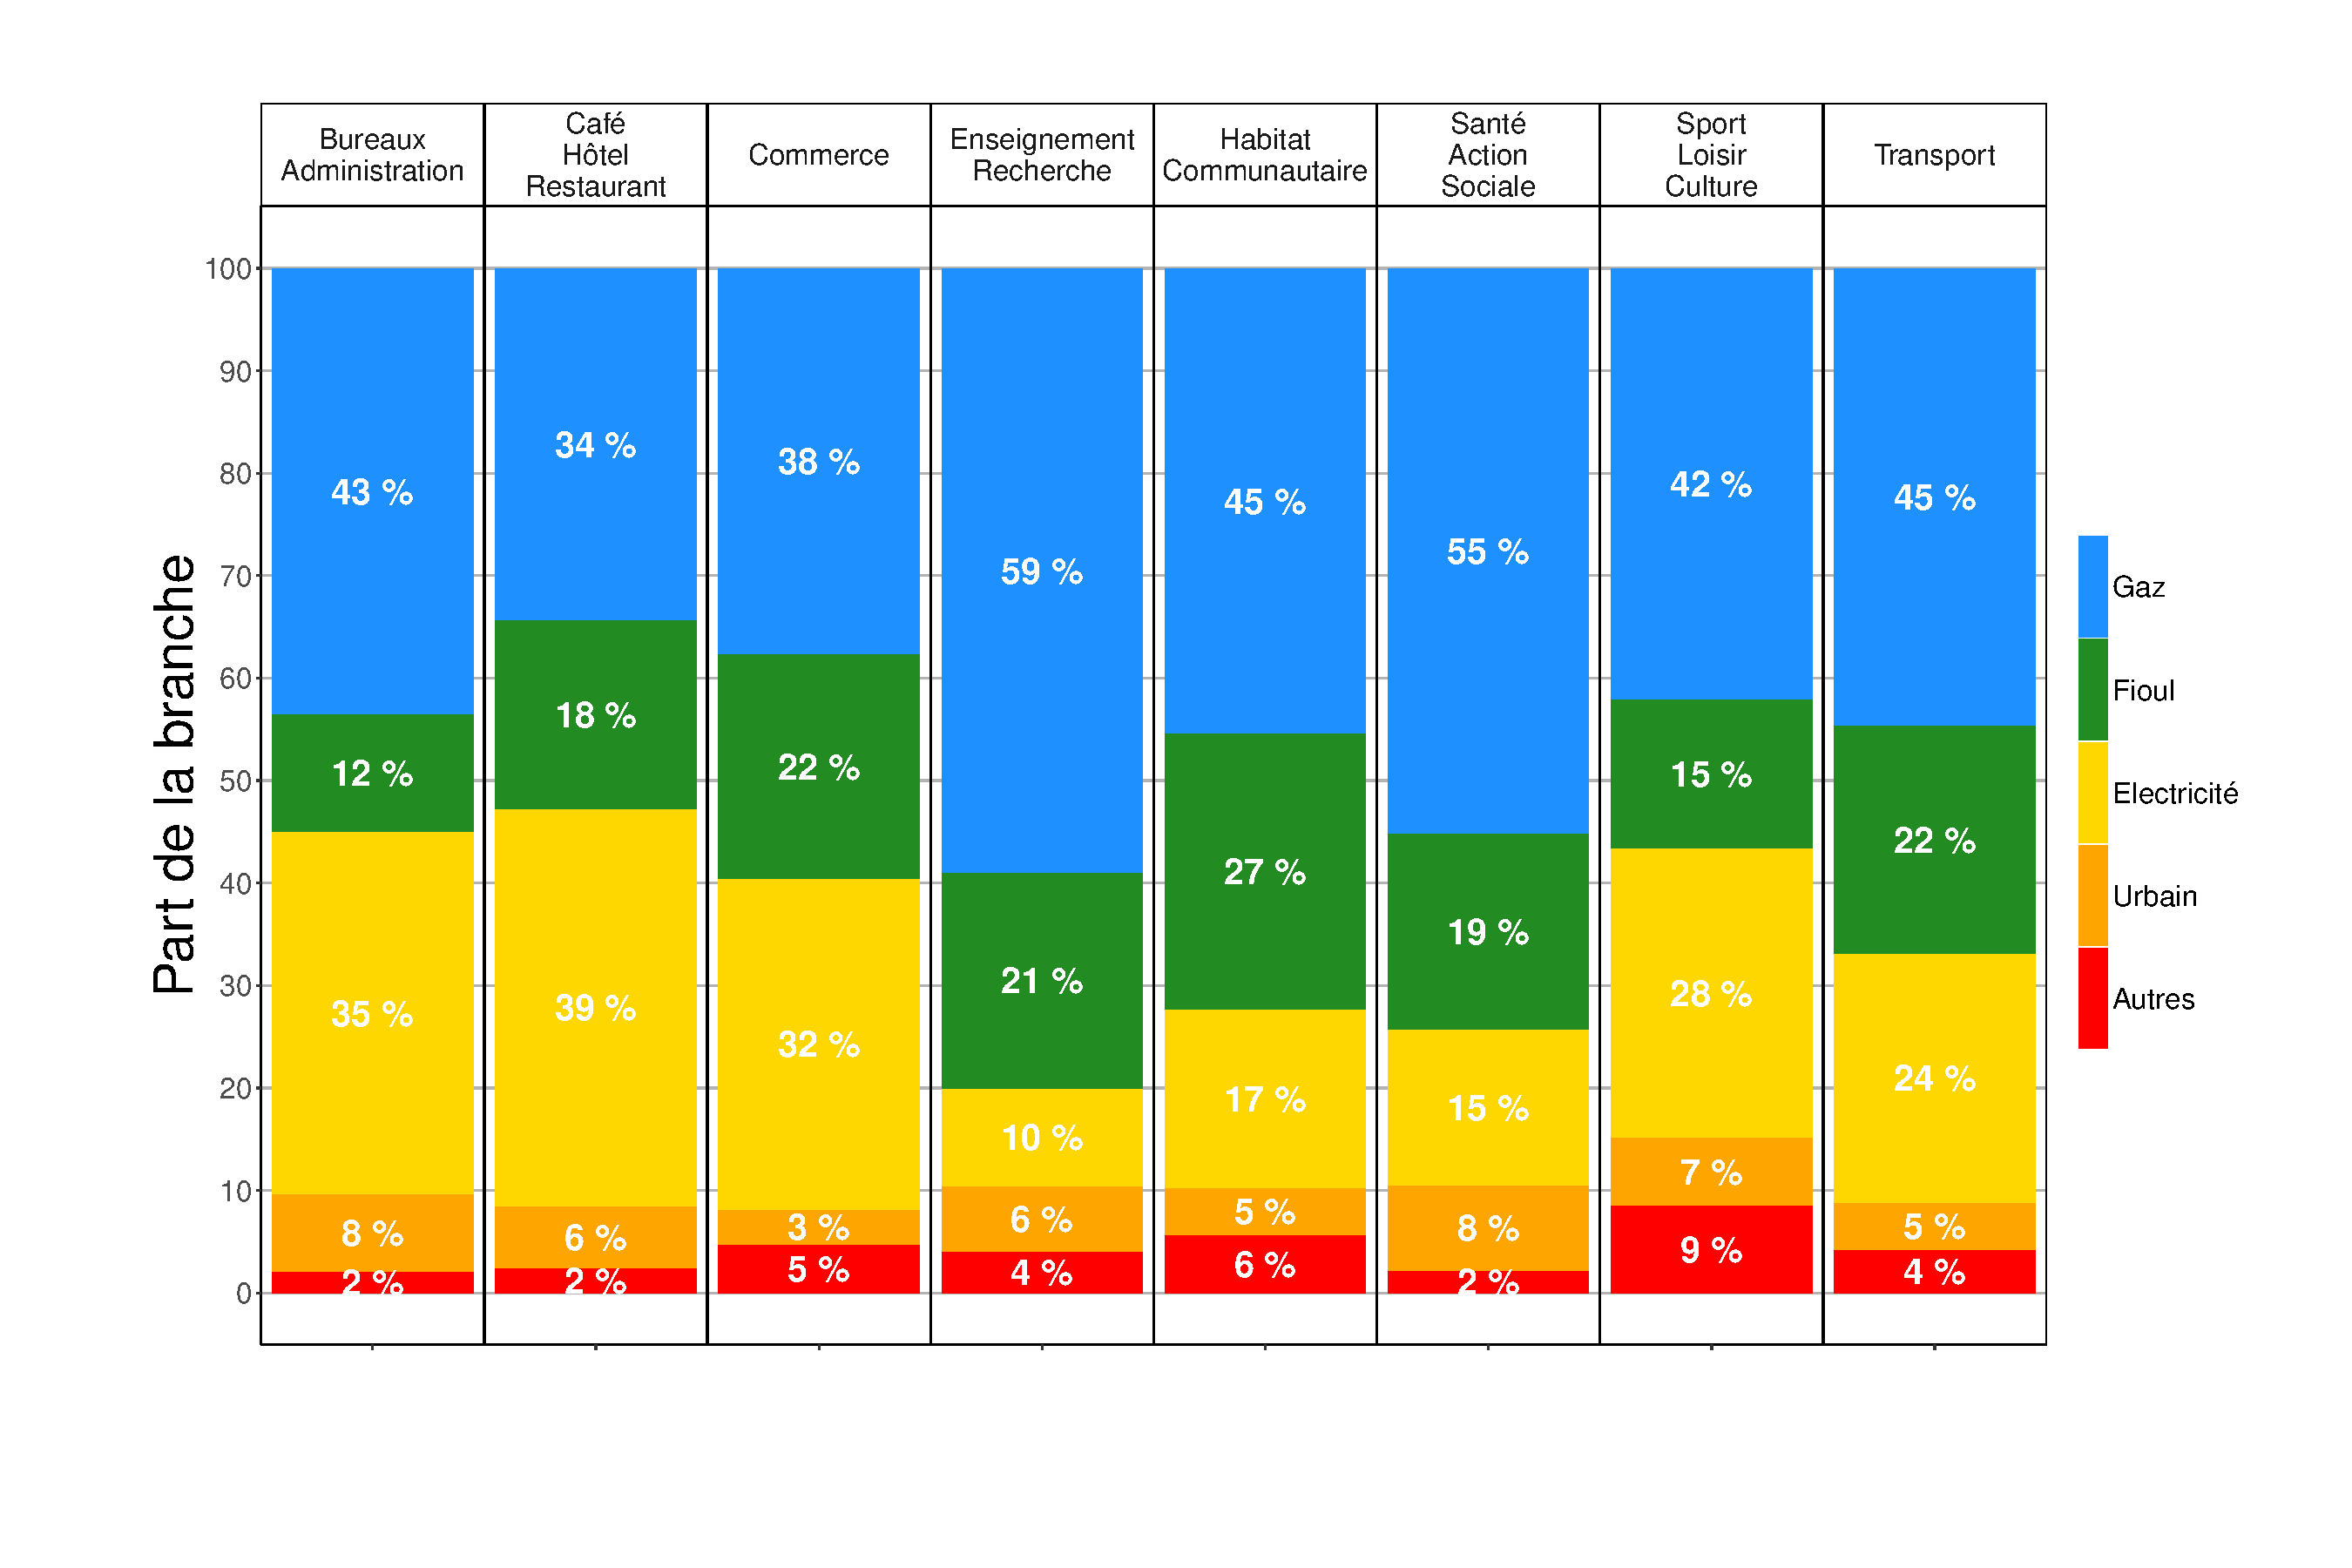
\includegraphics[width = 0.7\textwidth]{ParcEnergieBranche2010}
\end{figure}

\subsection{Subdivision du parc en \og bâtiment types \fg}

Pour caractériser plus finement le parc tertiaire et étudier les consommations d'énergie et les gisements d'économie d'énergie, un travail de définition de « bâtiments types » représentatifs pour chacune des activités tertiaires a été mené sur la base de travaux bibliographiques. 
Ces bâtiments types ont été construits selon l’activité exercée, la période de construction et la taille des établissements. La description de ces bâtiments comprend un plan masse, un découpage fonctionnel de l’espace interne (pièce par pièce), une description des matériaux de construction ainsi qu’une description des paramètres d’occupation par pièce (plages horaires d’occupation des pièces, besoins en ventilation, besoins en éclairage, apports internes liés aux équipements de bureautique et d’éclairage, apports internes liés aux occupants…). Les modes constructifs, les plans masse et les paramètres d’occupation sont le fruit d’un travail spécifique mené conjointement par le bureau d’études Tribu Energie, le CEP de l’Ecole des Mines de Paris et Energies Demain sur la base d’expertises internes et de recherches bibliographiques.

A titre d’exemple, la branche d’activité tertiaire « Habitat Communautaire» comprend cinq bâtiments types (maison de retraite médicalisée, maison de retraite non médicalisée, foyer, résidence universitaire et établissement de service à la personne) déclinés selon cinq périodes de construction (avant 1974, 1975-1982, 1983-1988, 1989-2000, après 2000) déterminant les matériaux constitutifs du bâti. Un exemple de plan masse est représenté sur la figure \ref{Plan_masse}

\begin{figure}[ht]
\centering
\caption{
Plan masse et description par pièce d’un niveau du bâtiment type \og Maison de retraite médicalisée\fg}\label{Plan_masse}
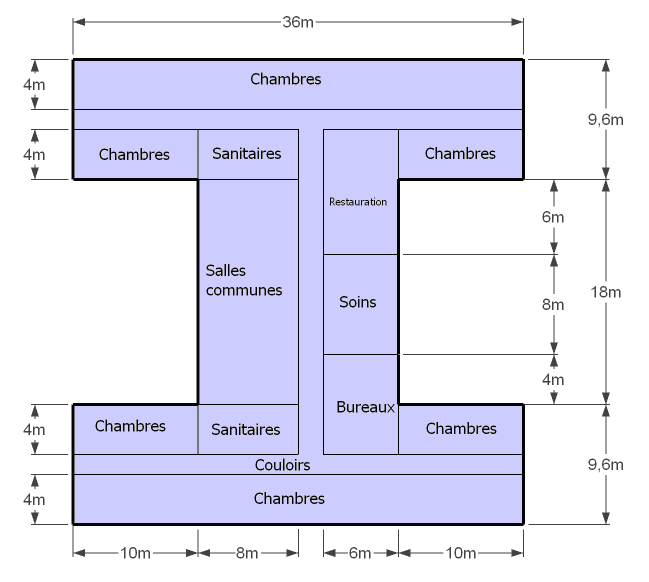
\includegraphics[width = 0.5\textwidth]{plan_masse}
\end{figure}

96 « bâtiments types » sont présents dans le modèle. Les surfaces tertiaires reconstituées précédemment sont ensuite subdivisées en « bâtiments types » directement par activité ou par implantation géographique (bâtiments de grande hauteur uniquement dans des zones densément peuplées, etc.).
\textbf{TODO Mettre la liste des bâtiments en annexe} 

\subsection{Calcul des besoins et des consommations unitaires des bâtiments}

Energies Demain et le CEP de l’Ecole des Mines de Paris ont développé une méthode de simulation et de reconstitution des consommations des bâtiments . Cette méthode de calcul est dite «~modulaire~» dans la mesure où elle se base sur une description physique du parc de bâtiments à l’échelle de la pièce (appelée aussi module), dans le but final de simuler pour chacune de celles-ci les besoins énergétiques et les puissances des systèmes requises par usage.

La première étape consiste à calculer les besoins unitaires par bâtiment. À partir de la description physique du parc en bâtiments types, les besoins en énergie par pièce et la puissance requise des systèmes de production par usage proviennent de simulations dynamiques (au pas de temps horaire) réalisées pour chacune des zones climatiques (8 zones climatiques d’hiver et 4 d’été). Les besoins par pièce, bâtiment type et zone climatique sont obtenus pour les usages suivants :

\begin{itemize}
	\item Chauffage
	\item Climatisation
	\item Auxiliaires de chauffage et climatisation
	\item Ventilation
	\item Éclairage
\end{itemize}

Les besoins et les puissances des systèmes calculés par pièce sont ensuite agrégés à l’échelle  du bâtiment type. À titre illustratif, cette méthode peut être comparée à l’assemblage d’un bâtiment en « empilant » les briques élémentaires que constituent chacune des pièces auxquelles sont associés les besoins et les puissances des systèmes calculés précédemment.

La seconde étape consiste à calculer les consommations unitaires en affectant des systèmes et des rendements associés aux bâtiments-types dont les besoins ont été simulés. 
On affecte à chacun des usages de l’énergie cités précédemment un système de production dont le dimensionnement et la performance sont issus de formules propres à chacun des systèmes. Il est à noter que ces formules sont paramétrables de manière à pouvoir moduler les performances des systèmes afin de les adapter au contexte territorial.
La répartition des systèmes de production est calée sur les données de cadrage disponibles~\footnote{Rapport du projet Optisol, ADEME/ARMINES, 2009. Rapport parlementaire sur la production de gaz à effet de serre des systèmes de climatisation et leur impact sur l’écosystème et l’environnement, Energies Demain et Armines, 2011}.

Enfin, les consommations unitaires des usages non simulés (cuisson, eau chaude sanitaire, bureautique et process) sont estimées sur la base de travaux nationaux et d’expertises internes \footnote{modèle CHARTER, \url{http://www.energies-demain.com/reseau/}. Maîtrise de la demande d’électricité et contrôle des courbes de charges, Energies Demain. Expertise complémentaire sur une meilleure identification des politiques énergétiques alternatives au projet Penly 3, Energies Demain. Étude des consommations énergétiques des bâtiments d’enseignement franciliens, Energies Demain}. L’ensemble des résultats de cet important travail a permis de constituer une bibliothèque de consommations unitaires, dépendantes du bâtiment type, de l’usage, de l’énergie, de la zone climatique ainsi que des différents types d’équipements (systèmes de chauffage, de climatisation, de ventilation, d’éclairage, ou de production d’Eau Chaude Sanitaire…). Les usages de l’énergie retenus sont :

\begin{itemize}
	
	\item Usages simulés (Simulations thermiques dynamiques) : 
	\begin{itemize}
		\item Chauffage
		\item Climatisation
		\item Auxiliaires de chauffage et de climatisation
		\item Ventilation
		\item Éclairage
  \end{itemize}
	\item Usages estimés sur travaux d'expertise : 
		\begin{itemize}
		\item Eau chaude sanitaire
		\item Cuisson
		\item Bureautique
		\item Froid alimentaire
		\item Process
		\item Autres
	\end{itemize}
\end{itemize}


Le schéma suivant illustre le cheminement correspondant. La première étape décrite ci-dessus est contenue dans l’encadrement pointillé « Simulation des besoins et des puissances de systèmes par pièce » (couleur violette).

\begin{figure}[ht]
\centering
\caption{ENERTER Tertiaire - Détermination des consommations unitaires}\label{Schema_calcul_conso}
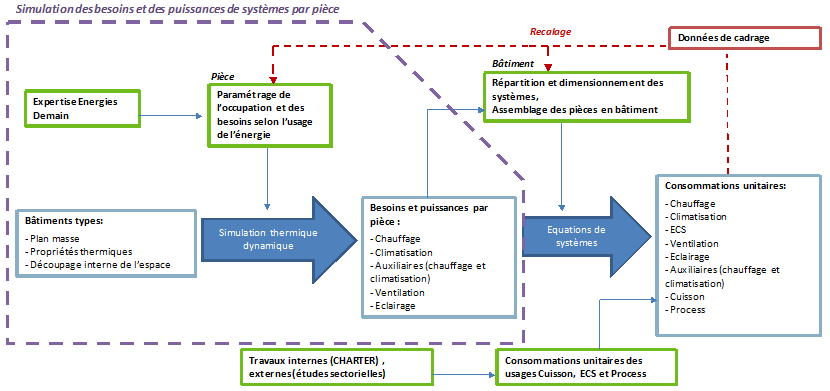
\includegraphics[width = 0.8\textwidth]{Schema_calcul_conso}
\end{figure}

\newpage
\clearpage


\subsection{Rendements des systèmes et consommations unitaires à l'état initial}

Pour chaque type de système de chauffage, deux types de performances existent dans le modèle. Les systèmes performants présentent un meilleur rendement que leur version classique (table \ref{Rdtsyst}). Les rendements varient d'un bâtiment-type à l'autre selon sa taille et la puissance demandée. 
 
La répartition des systèmes de chauffage issue de la reconstitution du parc est présentée sur la figure \ref{PMsyst2010}.  A l’état initial, on observe que les systèmes performants représentent une part très faible des systèmes installés. La majeure partie du parc est chauffée par des chaudières gaz et fioul traditionnelles. Les systèmes électriques (électrique joule, PAC, DRV, Rooftop...) répresentent seulement 23~\% des systèmes. Le rendement moyen des systèmes de chauffage sur le parc en 2010 est de 0,8 ce qui est proche de celui des chaudières gaz classiques. 
 
\begin{table}[ht]
\caption{Rendements moyens des systèmes de chauffage dans le modèle}
\label{Rdtsyst}
\begin{center}
\begin{tabular}{l|c}

\textbf{Système}	&	\textbf{Rendement moyen}
\\	\hline	\\	
Chaudière gaz	& 0,76 \\	
Chaudière condensation gaz	& 0,98 \\	
Chaudière fioul & 0,64 \\	
Chaudière condensation fioul	& 0,75 \\	
Electrique direct	& 0,92 \\	
Electrique direct performant	& 1,00 \\	
PAC	& 3,00 \\	
PAC performant	& 3,30 \\	
Rooftop	& 2,80 \\	
Rooftop performant	& 3,3 \\	
Tube radiant	& 0,84 \\	
Tube radiant performant	& 1,00 \\	
Cassette rayonnante	& 0,84 \\	
Cassette rayonnante performant	& 1,00 \\	
DRV	& 2,50 \\	
DRV performant	& 3,20 \\	
Autre système centralisé (Bois)	& 1,20 \\	
Autre système centralisé (Urbain) & 1,00 \\	
Autre système centralisé performant	(Bois) & 1,30 \\	
Autre système centralisé performant	(Urbain)& 1,30 \\	
\hline	
\end{tabular}
\end{center}

\textbf{\footnotesize{NB : les valeurs de rendement indiquées ici sont des valeurs moyennes sur l'ensemble du parc. Les rendements peuvent différer fortement selon le type de bâtiment dans le modèle en fonction de la puissance demandée et de la taille du bâtiment. La catégorie~\og~Autre système centralisé~\fg~correspond aux systèmes fonctionnant au bois, au GPL ou au chauffage urbain. }}
\end{table}

\begin{figure}[ht]
\centering
\caption{Parts de marché des systèmes de chauffage dans le modèle en 2010}\label{PMsyst2010}
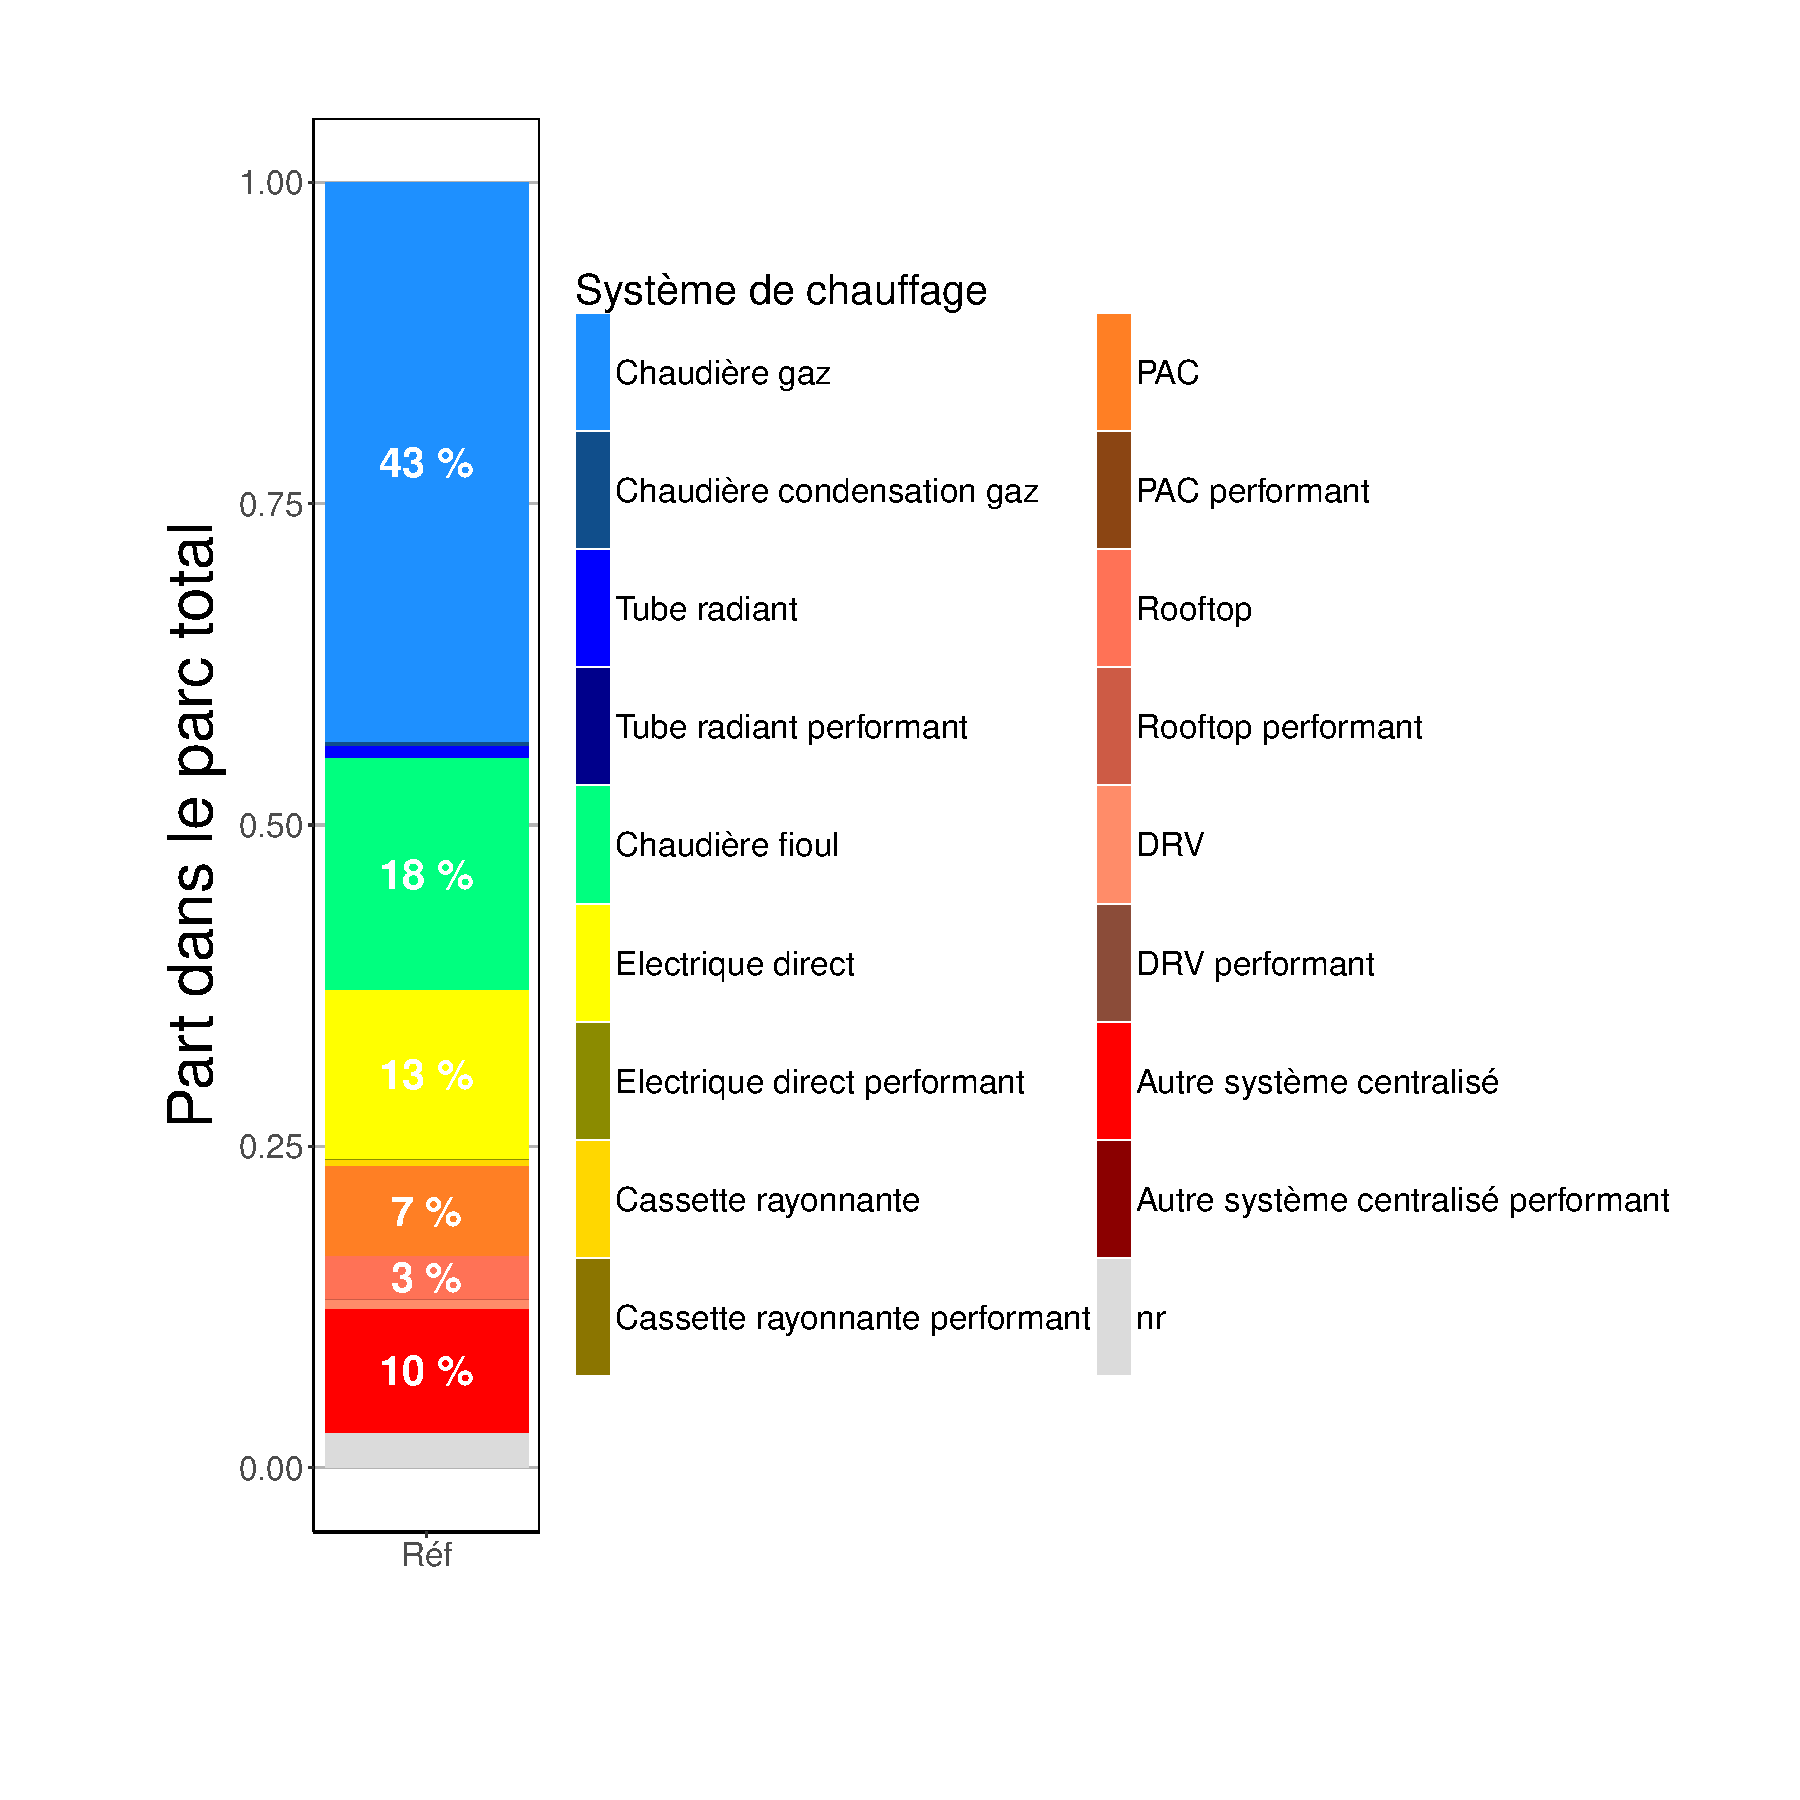
\includegraphics[width = 0.5\textwidth]{PMsyst2010} 
\end{figure}

Pour l'eau chaude sanitaire, les rendements ne dépendent pas du type de bâtiment mais de l'énergie utilisée et du type de système (classique ou performant, cf table \ref{RdtsystECS}) \footnote{Les besoins en eau chaude dépendent eux du bâtiment}. A l'état initial, le rendement moyen des systèmes d'ECS est de 0,7 du fait de la distribution des énergies dans le parc. Les systèmes performants représentent une part très faible des systèmes. 

\begin{table}[ht]
\caption{Rendements moyens des systèmes d'ECS dans le modèle}
\label{RdtsystECS}
\begin{center}
\begin{tabular}{l|l|c}
\textbf{Énergie}	& \textbf{Système}	&	\textbf{Rendement moyen}
\\	\hline	\\	
Électricité	 & Ballon &  0,9\\	
Gaz	& Chaudière ou ballon & 0,7\\	
Fioul	& Chaudière & 0,5\\	
Urbain	& Système performant &  0,55\\	
Autres	& Chaudière & 0,55 \\	
Électricité	 & Ballon thermodynamique	& 2.5 \\	
Gaz	& Chaudière ou ballon condensation	& 0.9 \\	
Fioul	& Chaudière condensation	& 0.8 \\	
Urbain	& Système performant	& 0.8 \\	
Autres	& Chaudière condensation	& 0.8 \\	
\hline	
\end{tabular}
\end{center}
\end{table}

Pour la climatisation, le rendement pour un type de bâtiment dépend du type de système installé (DRV, Rooftop, PAC ou groupe ancien). La part des systèmes variant selon la branche d'activité, les rendements peuvent aussi varier d'une branche à l'autre. A l'état initial, le rendement moyen des systèmes de climatisation est de 3,05. Pour tous les autres usages (essentiellement électriques sauf la cuisson), les besoins unitaires sont égaux aux consommations en énergie finale. 

En appliquant ces rendements au besoins unitaires par usages imputées aux différents bâtiments-types, on obtient les consommations unitaires en énergie finale par usage présentées dans le tableau \ref{ConsoU_usage}. Les consommations unitaires moyennes du parc sont de 247 kWhEF/m² en 2009. Les usages couverts par la réglementation thermique (usages réglementés) représentent plus de 80~\% des consommations unitaire du parc (200 kWhEF/m² environ). Le chauffage représente le plus gros poste de consommation. L'éclairage et l'ECS représentent 1/5 des consommations unitaires. 

\begin{table}[h!]
\caption{Consommations unitaires moyennes (kWhEF/m²) par usage en 2009 dans le modèle }
\label{ConsoU_usage}
\begin{center}
\begin{tabular}{l|c}
\textbf{Usage}	& \textbf{Consommation unitaire}	
\\	\hline	\\	
Usages réglementés : &  
\\	 \hline	
Chauffage         &    122,4 \\
ECS                &    23,8 \\
Climatisation     &      6,0 \\
Ventilation      &       7,2 \\
Auxiliaires     &        5,4 \\
Éclairage          &    27,0 \\
Bureautique      &      10,0 \\
\hline	\\	
Usages non réglementés : & 
\\	\hline	
Cuisson            &    15,1 \\
Froid alimentaire  &     8,6 \\
Process            &     4,5 \\
Autre           &       16,8 \\
\hline	
\end{tabular}
\end{center}
\end{table}

Les consommations unitaires varient d'une branche d'activité à l'autre (figure \ref{Conso_u_Branche}). En effet, si le chauffage reste le poste de consommation le plus important dans toutes les branches, certaines branches présentent des spécificités comme l'hôtellerie avec de fortes consommations de cuisson et d'ECS, les commerces et les transports avec de fortes consommations d'éclairage ou les bureaux avec leur forte consommations d'électricité pour la bureautique.

\begin{figure}[ht]
\centering
\caption{Consommations unitaires par usage et par branche d'activité en 2009}\label{Conso_u_Branche}
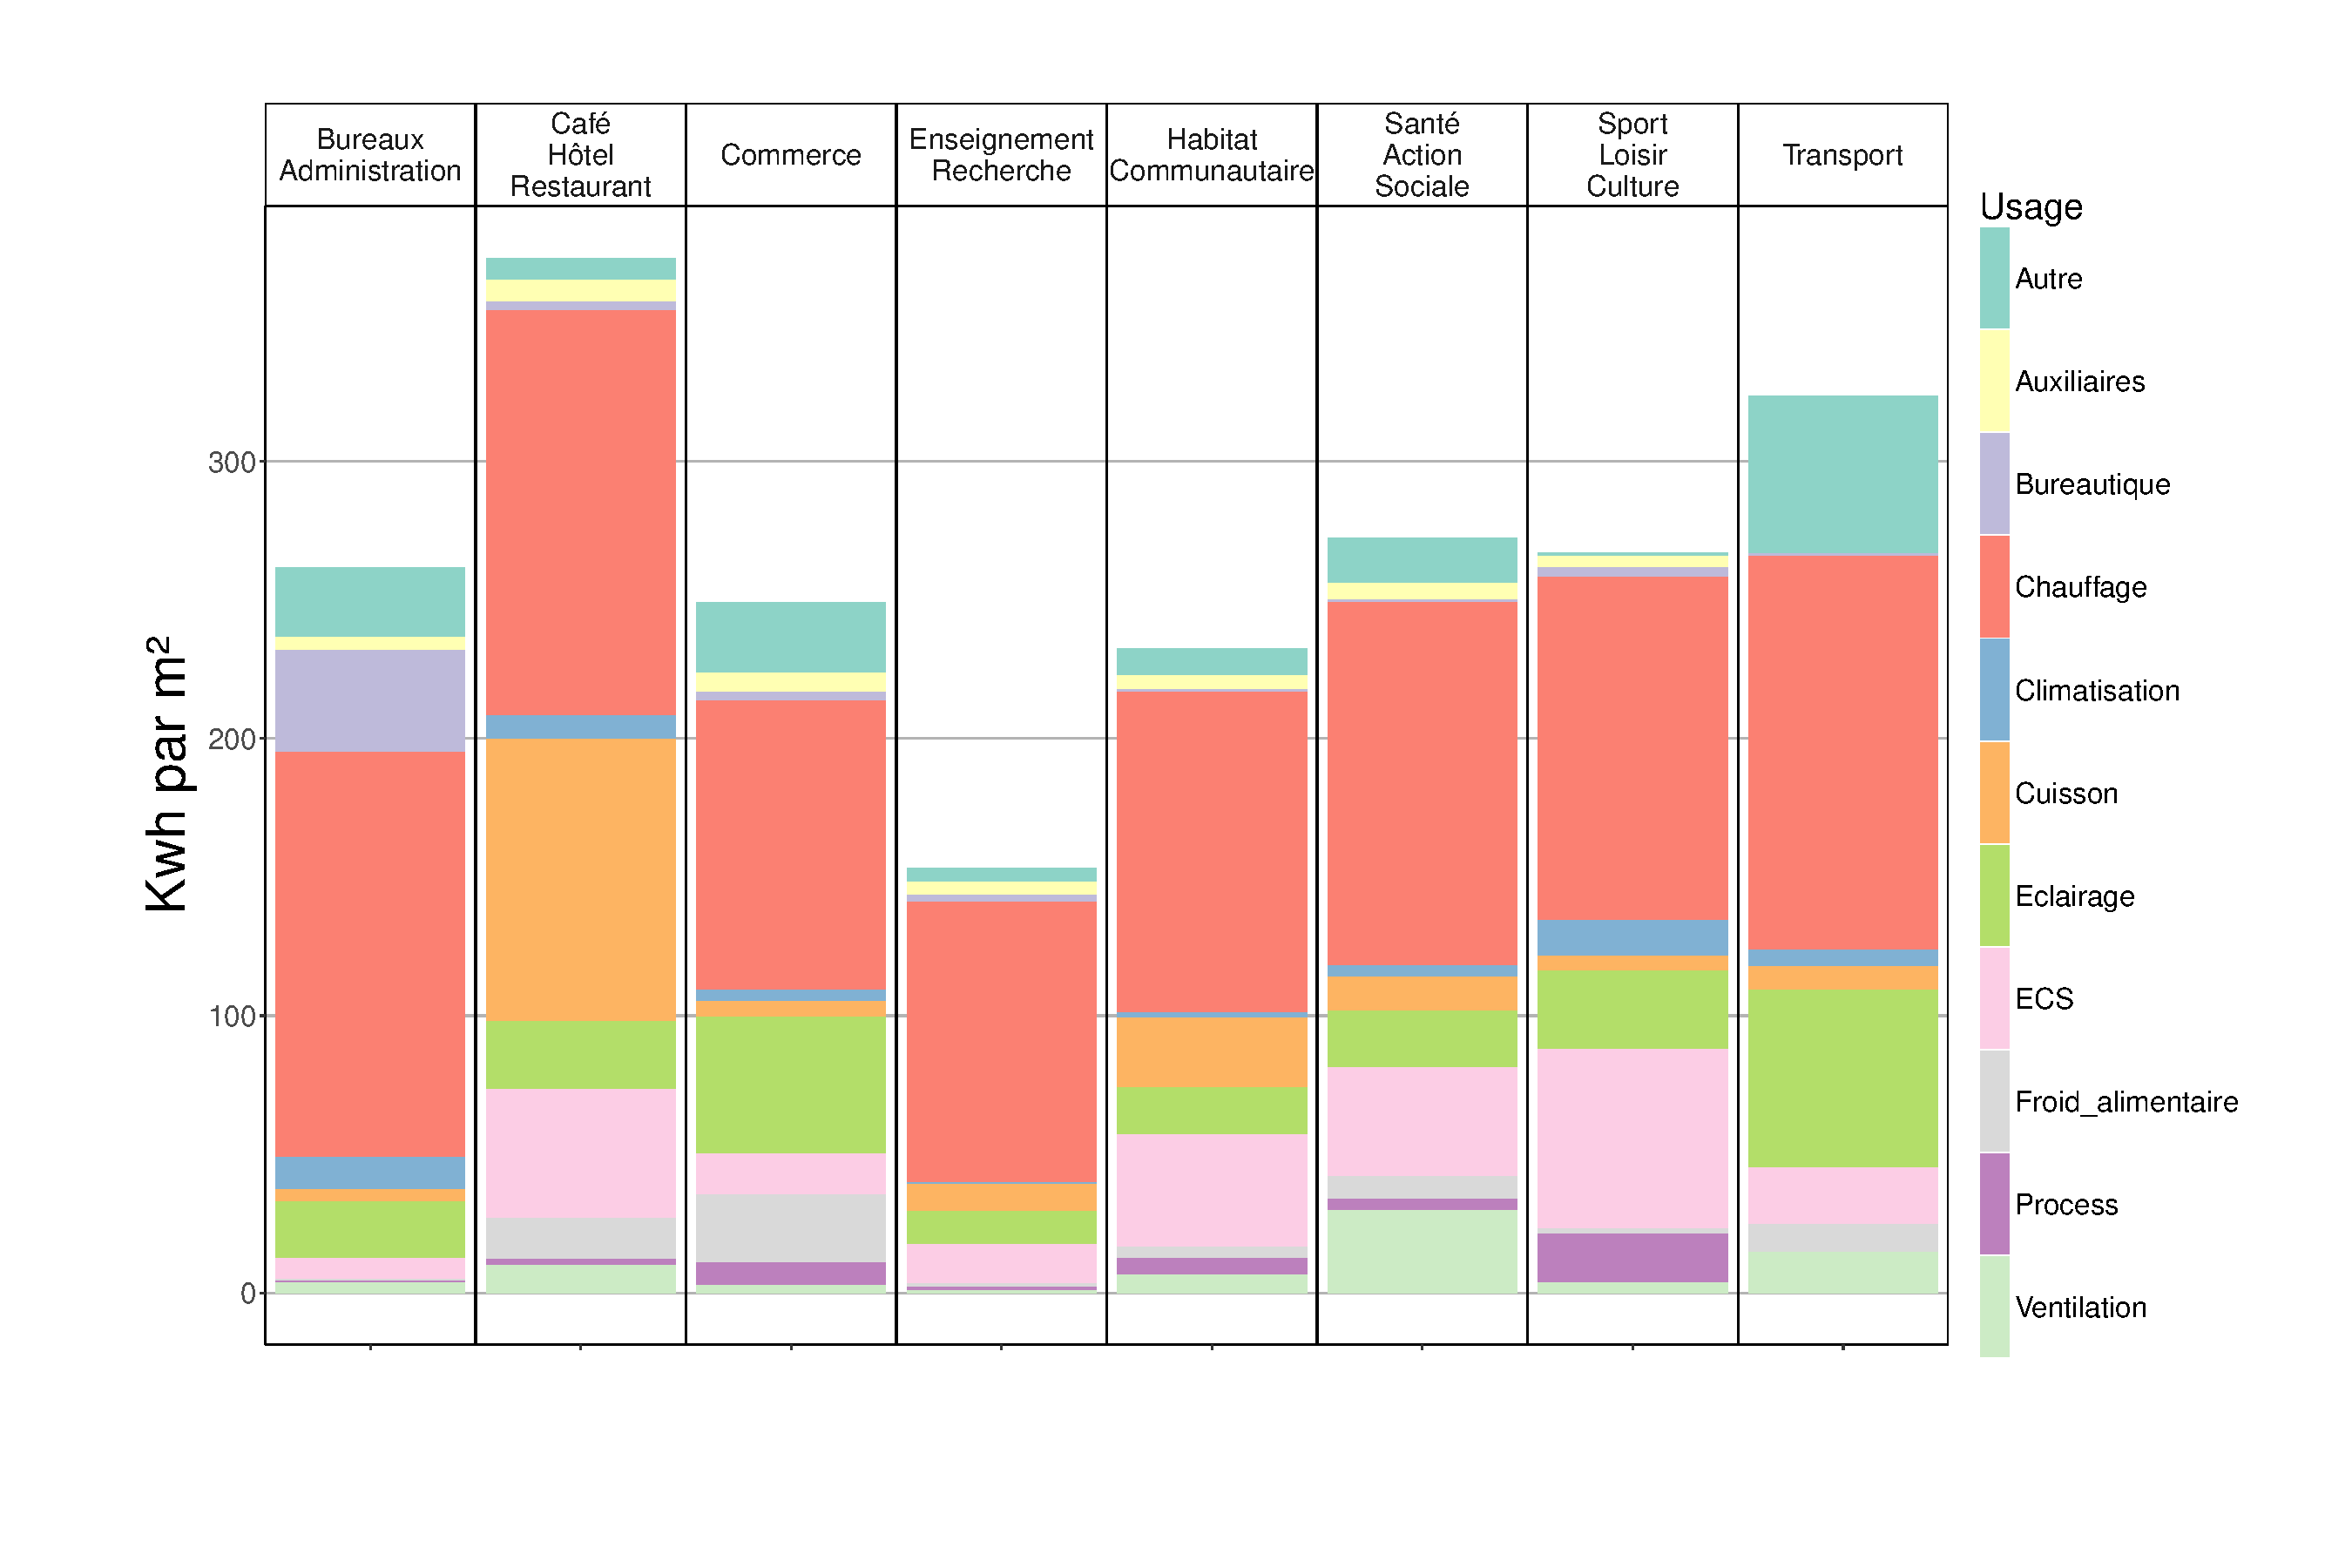
\includegraphics[width = 0.7\textwidth]{Conso_u_Branche} 
\end{figure}

\subsection{Performance énergétique du parc à l'état initial}

Pour les bâtiments du secteur tertiaire, il existe plusieurs types de DPE (Diagnostic de performance énergétique) en fonction de l’activité : un pour les centres commerciaux, un pour les bureaux et l'enseignement, un pour les bâtiments à usage continue comme les hôpitaux et un pour les autres activités. L'échelle des étiquettes énergie (bornes des étiquettes en kWhEP par m²) est différente en fonction du type de bâtiment. Pour attribuer une étiquette énergie aux bâtiments représentées dans le modèle, on calcule les consommations en kWhEP par m² pour les usages réglementés pour chaque type de bâtiment et on les compare à l'échelle DPE correspondante. A l'état initial, un même type de bâtiment peut avoir plusieurs étiquettes selon sa période de construction, les systèmes installés et l'énergie utilisée.  

la figure \ref{Parcetiqbranche} présente la performance énergétique du parc par branche d'activité en 2009. La distribution des étiquettes énergie révèle des disparités entre secteurs. En effet, les branches d’activité Enseignement/Recherche, Habitat communautaire et Santé/Action sociale sont  plus performantes.

\begin{figure}[ht]
\centering
\caption{Performance énergétique du parc par branche d'activité en 2009}\label{Parcetiqbranche}
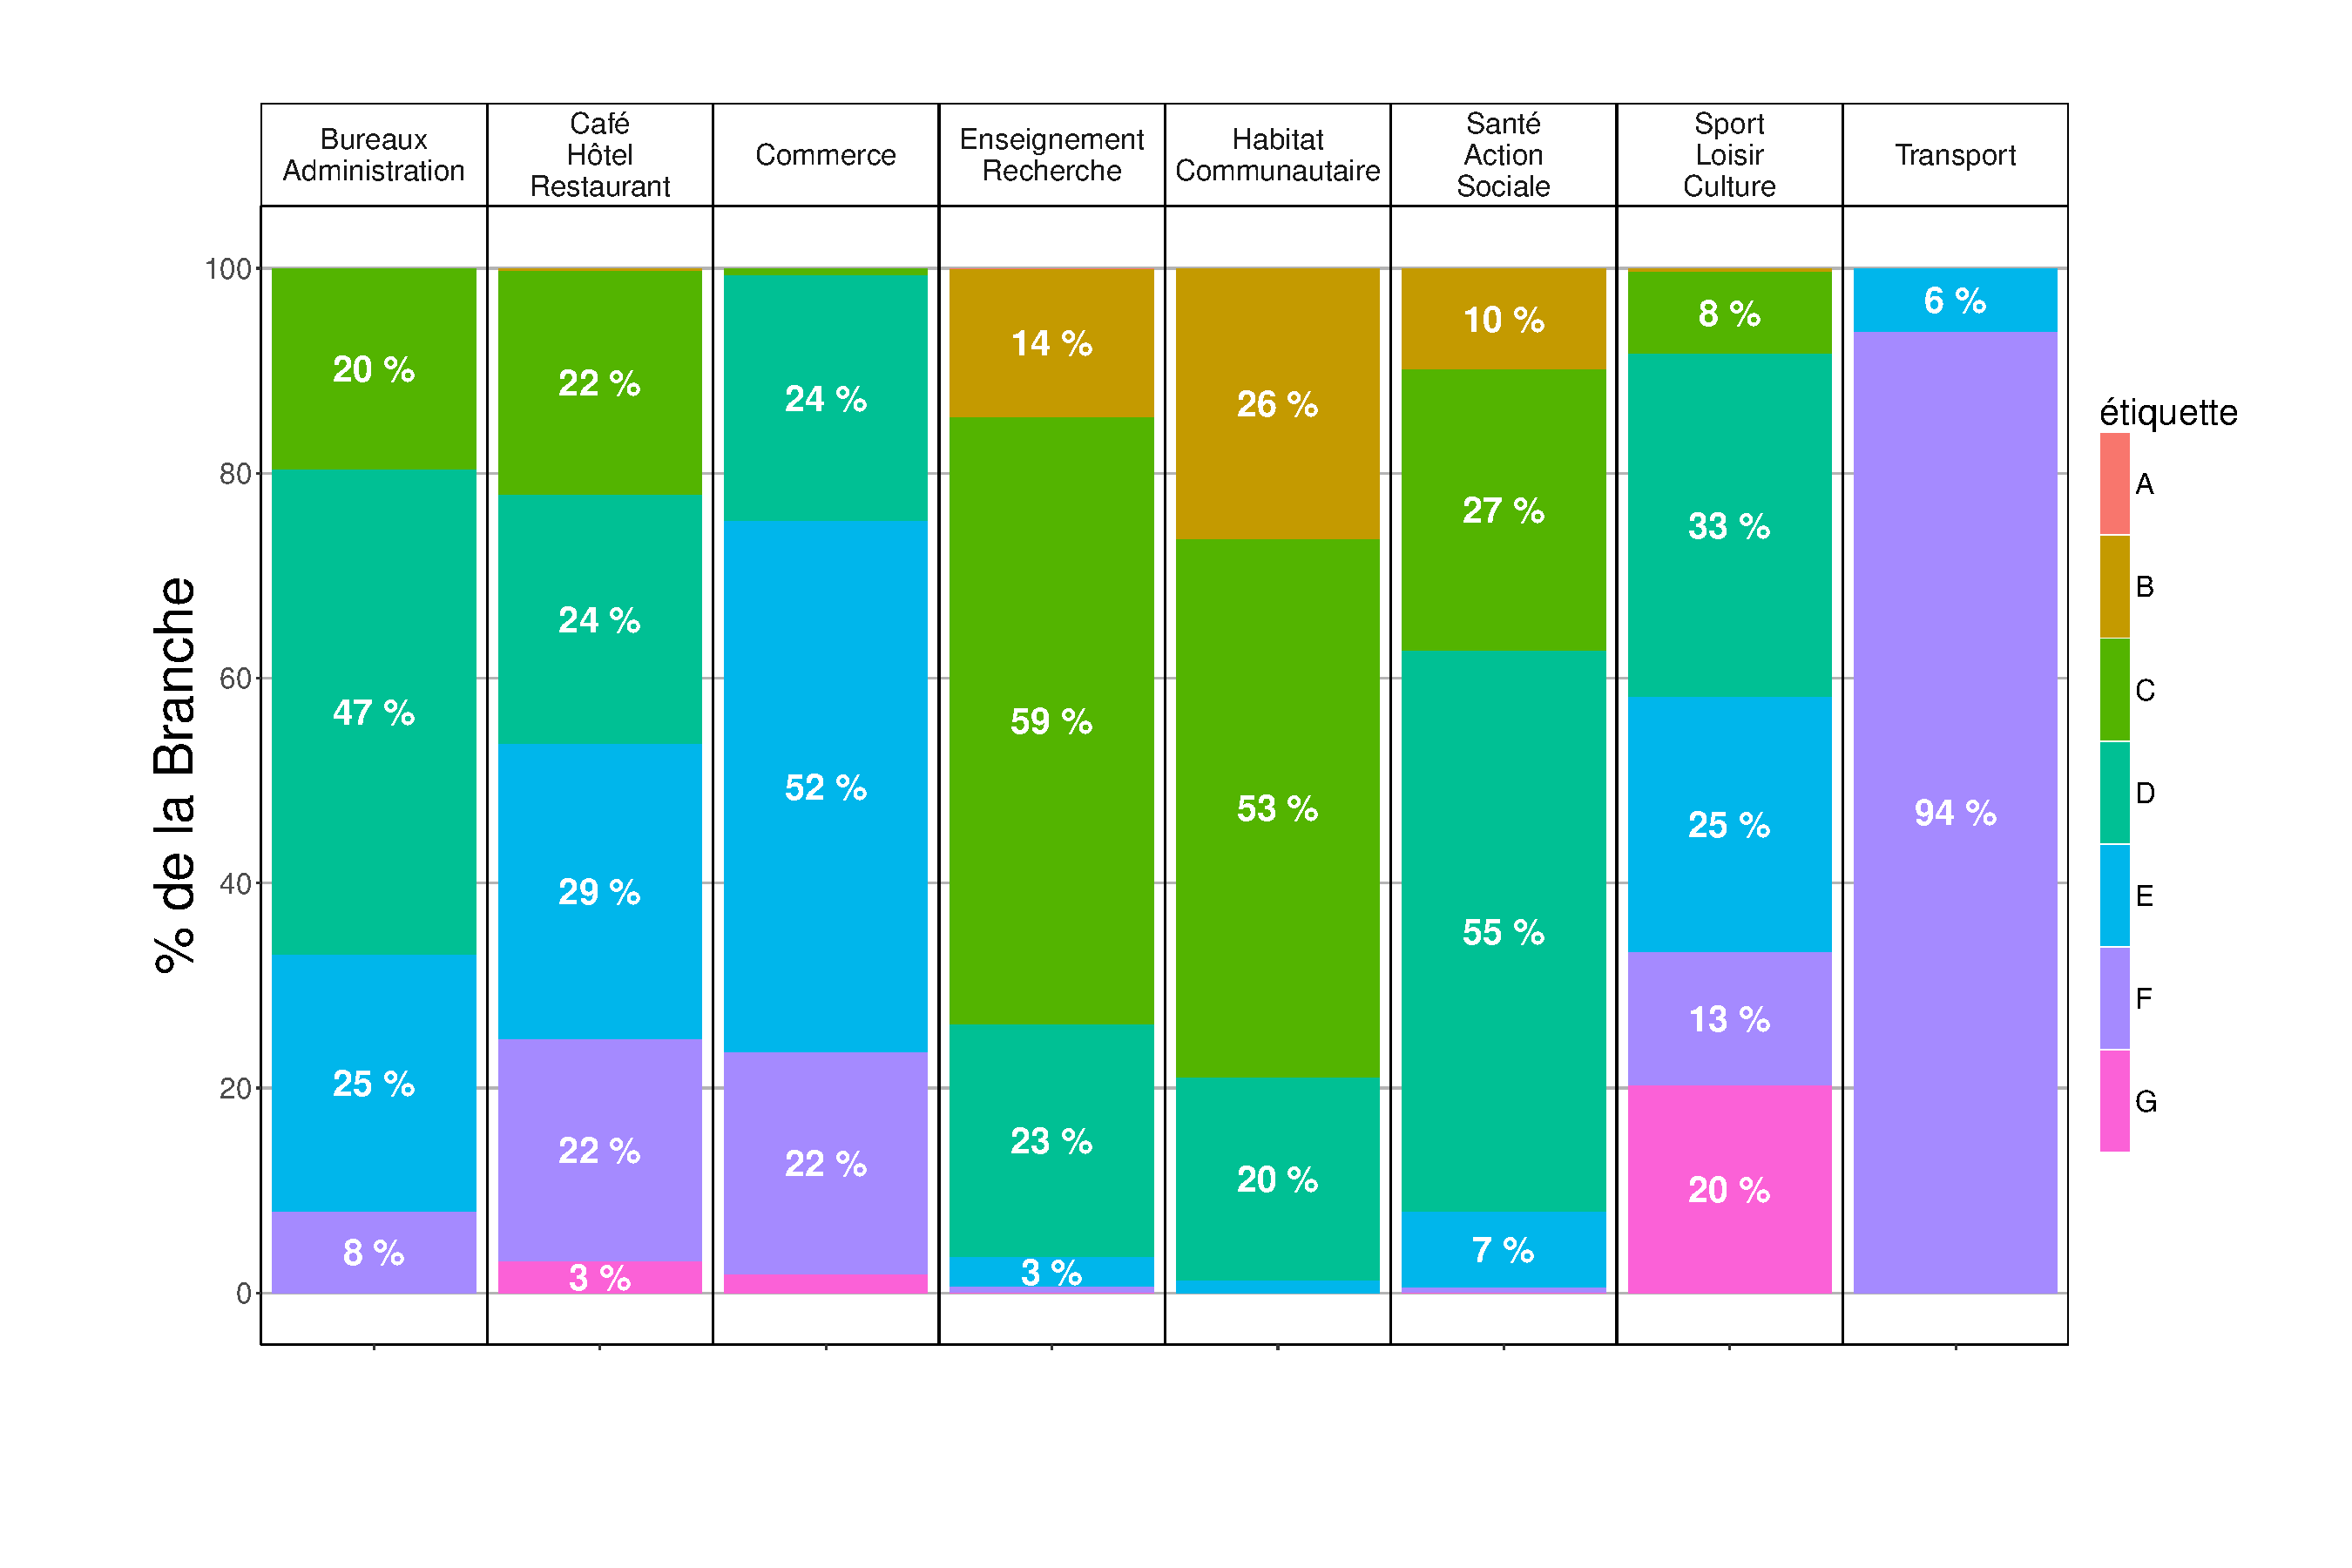
\includegraphics[width = 0.7\textwidth]{Parcetiqbranche} 
\end{figure}

\newpage
%\clearpage

\subsection{Aggrégation des consommations à l'échelle du parc tertiaire}

La reconstitution des consommations du parc à l'échelle nationale est le fruit de l’affectation des consommations unitaires à chaque établissement du parc bâti tertiaire décrit précédemment. Cette affectation se fait selon la nature de l’activité tertiaire exercée, la période de construction et les caractéristiques des systèmes de production (type de chauffage, de climatiseur, de ventilation, d’éclairage…). Les consommations obtenues font ensuite l’objet d’un calage à l’échelle nationale et régionale sur la base de données de cadrage disponibles (CEREN, données issues de travaux d'expertise précédents d'Energies Demain...). 

A l'échelle nationale, les consommations totales par vecteur énergétique dans le modèle correspondent bien à celles des données du CEREN en 2010 (figure \ref{CompConsoTot2010}).  Les consommations totales du parc sont de 225 TWh en 2010. L'électricité représente 45~\% des consommations, le gaz 32~\%, le fioul 16 ~\% et les autres combustibles (chaleur, biomasse et solaire). 
 
\begin{figure}[ht]
\centering
\caption{Comparaison des consommations totales du parc dans le modèle avec les données de consommations du CEREN (2010) }\label{CompConsoTot2010}
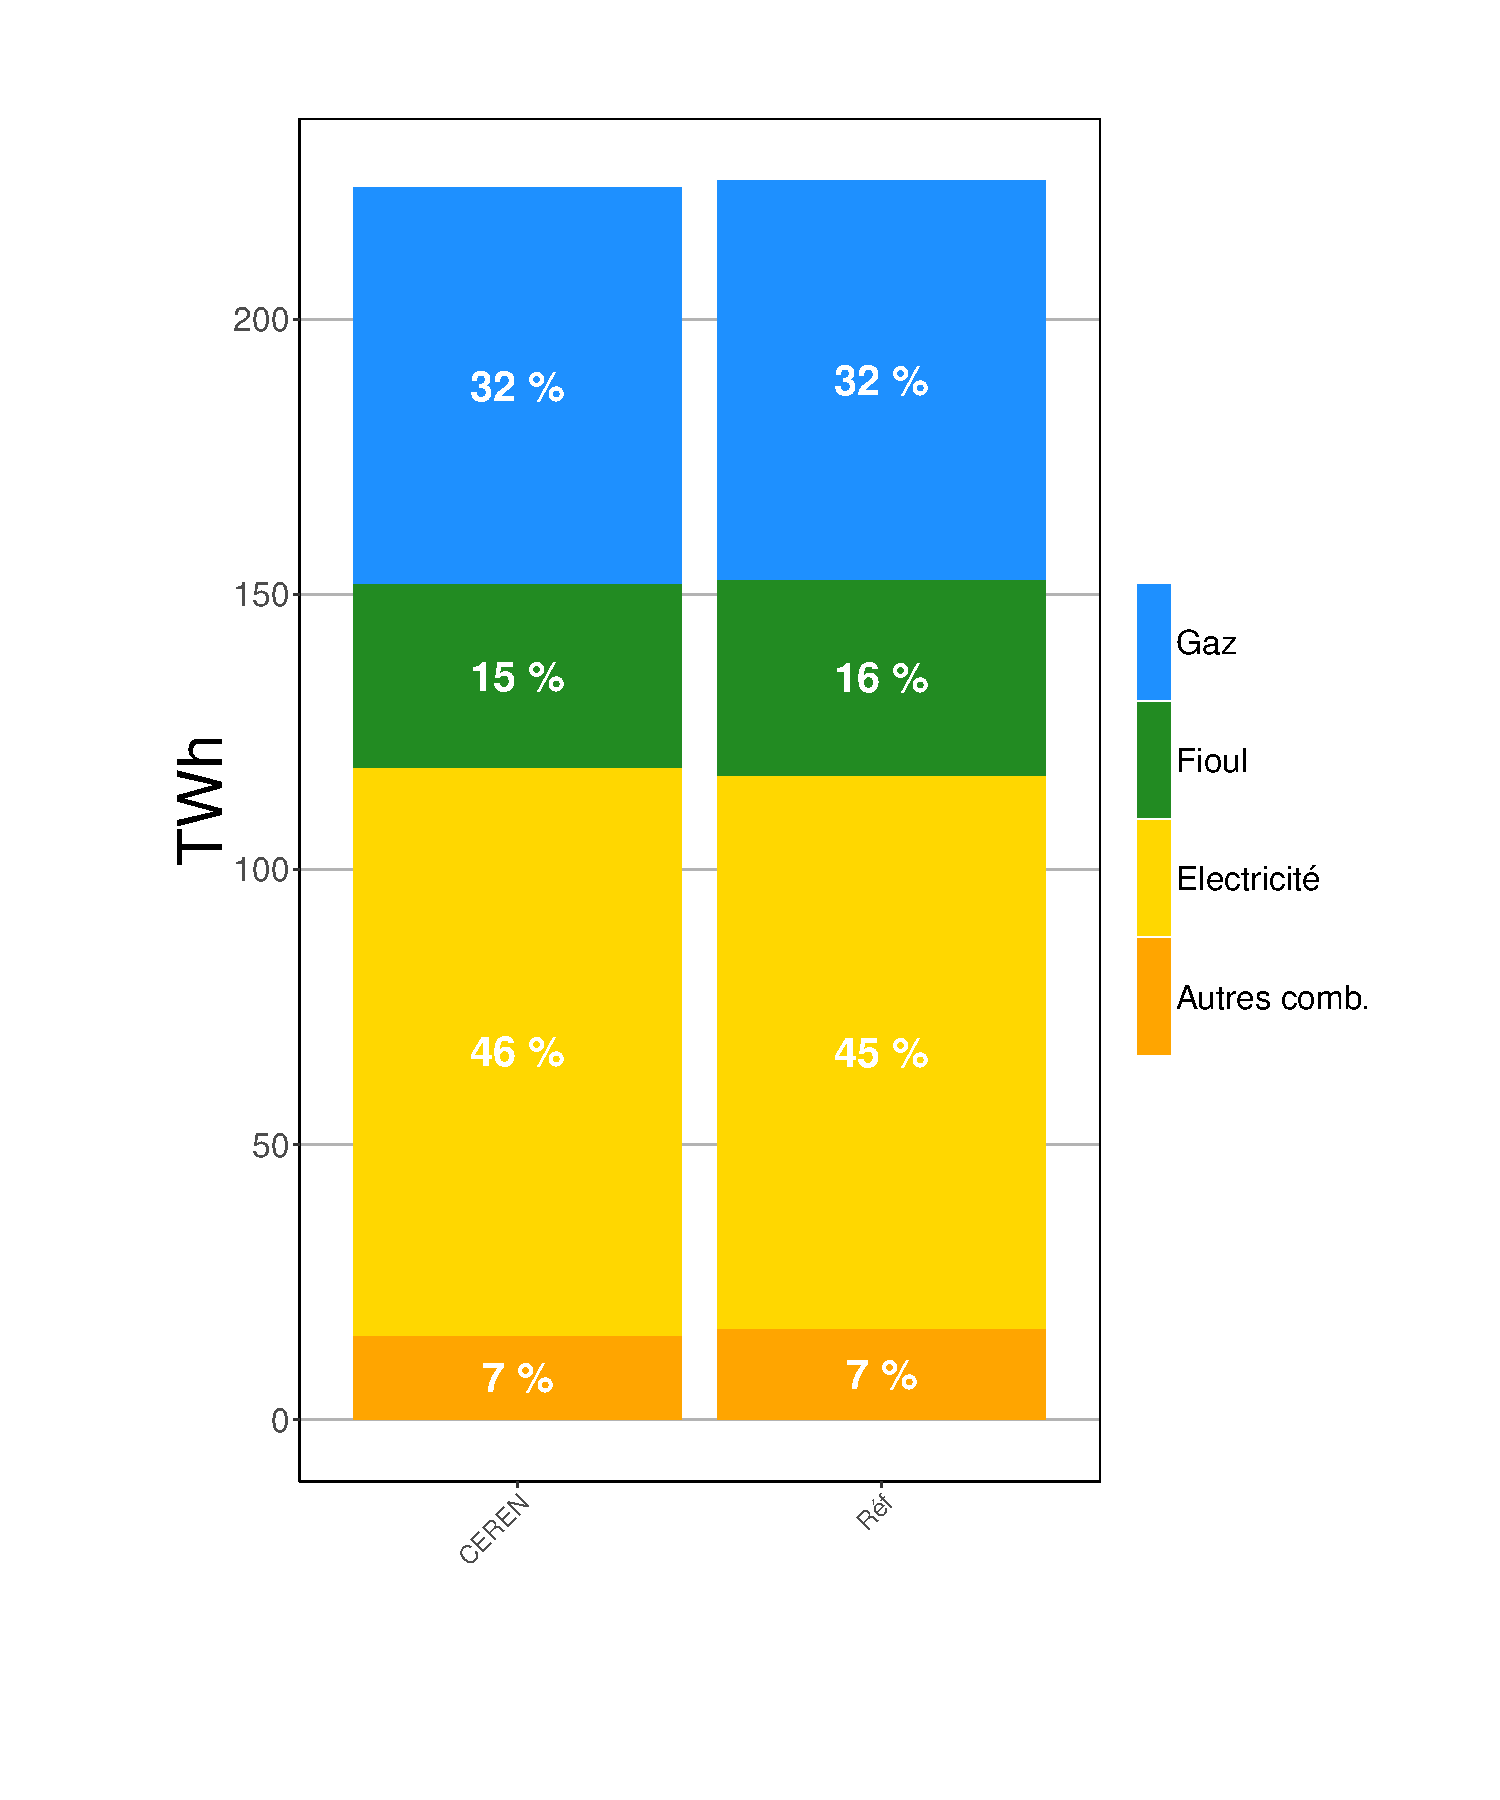
\includegraphics[width = 0.5\textwidth]{CompConsoTot2010}
\end{figure}

La répartition des consommations par usage et par vecteur énergétique diffère légèrement entre les données d'entrée du modèle et celles du CEREN. La répartition des consommations d'électricité entre les usages spécifiques et les autres usages est notamment sensiblement différente (figure \ref{CompConsousage2010}). Ceci provient notamment de différences méthodologiques dans la répartition des consommations d'électricité entre les usages. 

\begin{figure}[h!]
\centering
\caption{Comparaison des consommations par usage et par énergie du parc dans le modèle avec les données de consommations du CEREN (2010) }\label{CompConsousage2010}
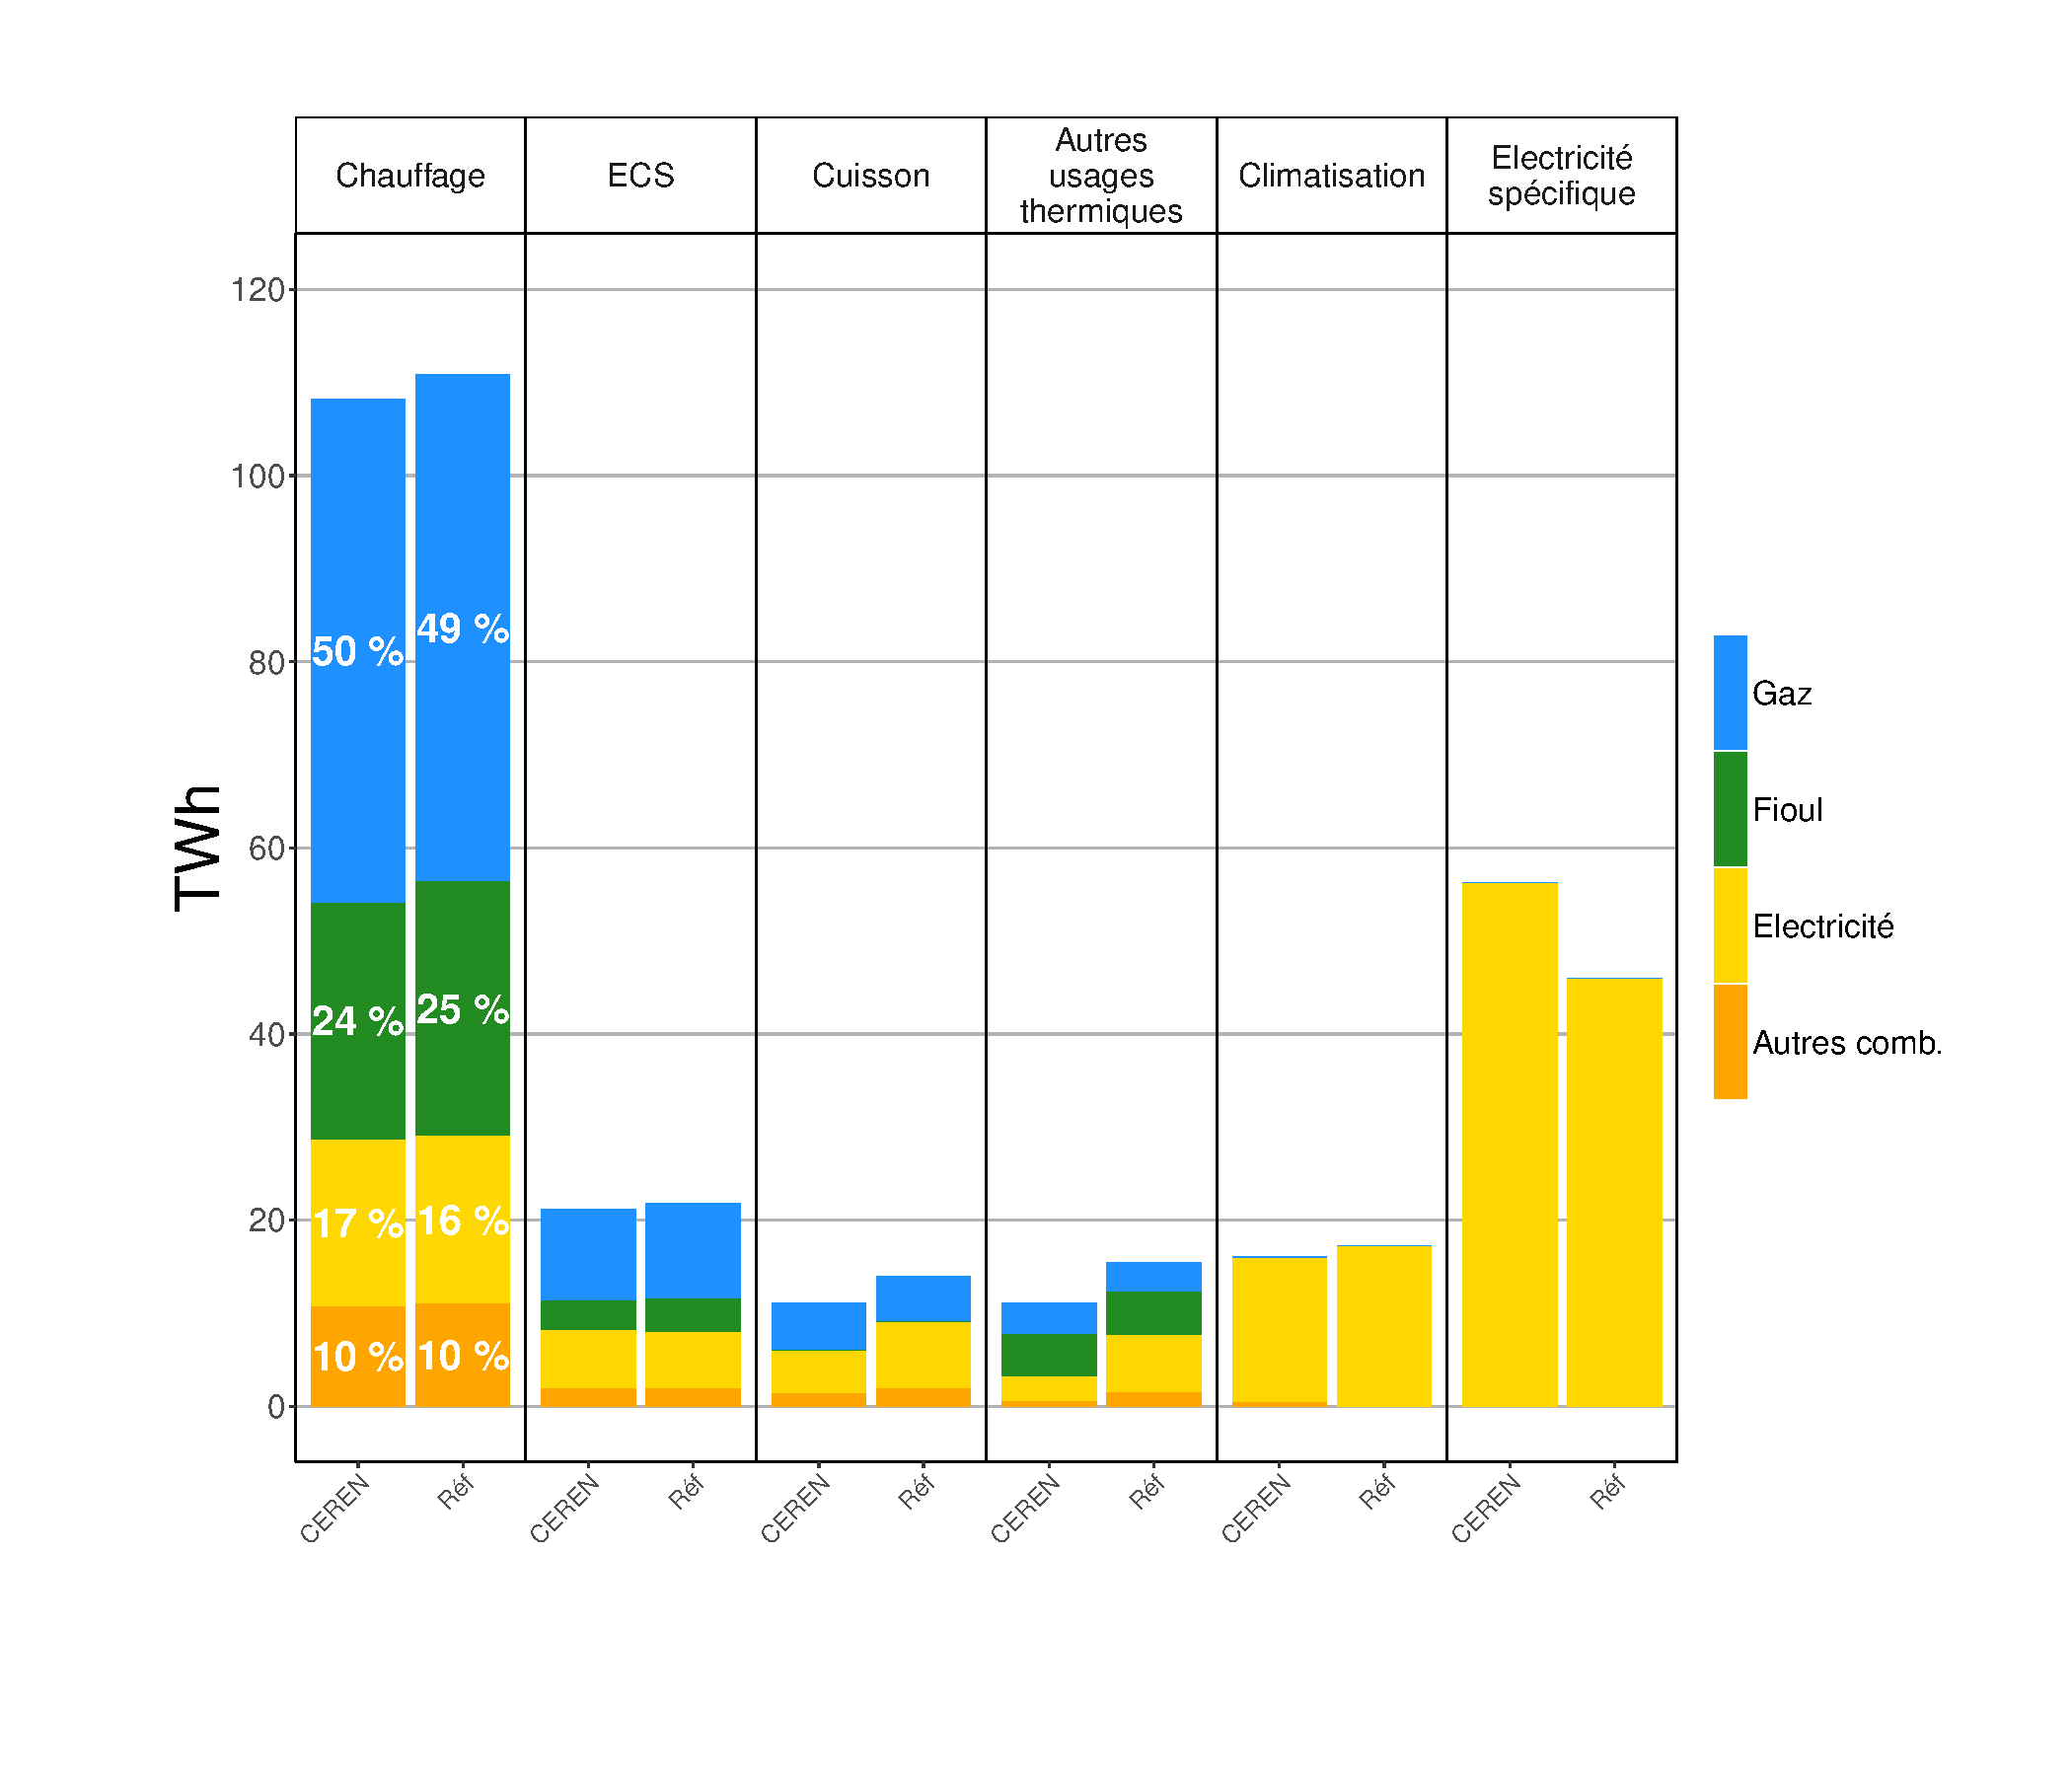
\includegraphics[width = 0.5\textwidth]{CompConsousage2010}
\end{figure}

La moitié des bâtiments tertiaires est chauffée au gaz en 2010 (figure \ref{CompConsousage2010}). L'électricité représente une part assez faible des consommations de chauffage (16~\% ). 
La majeure partie des consommations d'électricité du parc tertiaire provient des usages spécifiques de l'électricité (bureautique, éclairage, ventilation, auxiliaires, froid alimentaire et process) et de la climatisation. Sur 100 TWh d'électricité, ces usages représentent 45 TWh, le chauffage électrique 18 TWh et l'ECS 6 TWh.

Le chauffage représente 49~\% des consommations du parc tertiaire (figure \ref{ConsoBrancheusage2010}). L'ECS, la cuisson et les autres usages thermiques de l'énergie représentent 23~\% des consommations, les usages spécifiques de l'électricité et la climatisation 28~\%. Les deux branches du parc les plus énergivores sont les bureaux et les commerces. 

\begin{figure}[h!]
\centering
\caption{Distribution des consommations par branche et par usage dans le modèle en 2010}\label{ConsoBrancheusage2010}
\begin{tabular}{cc}
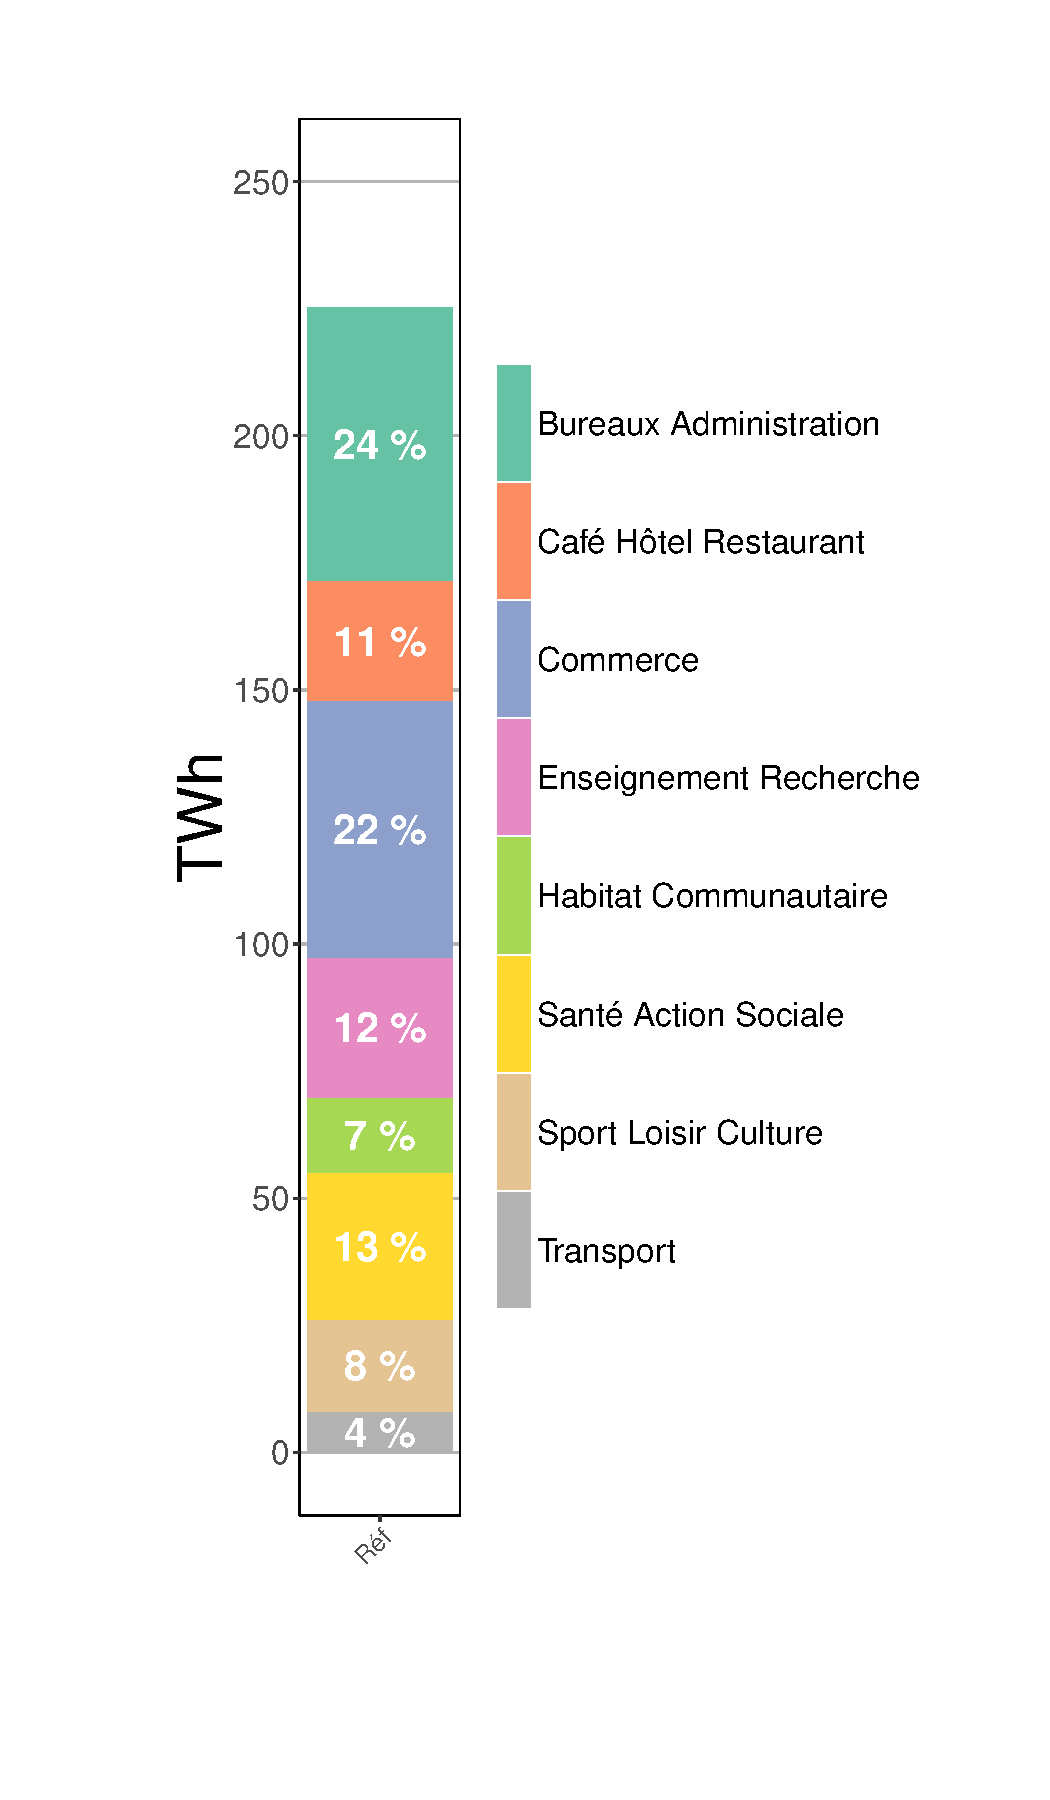
\includegraphics[width = 0.35\textwidth]{Consobranche2010}  & 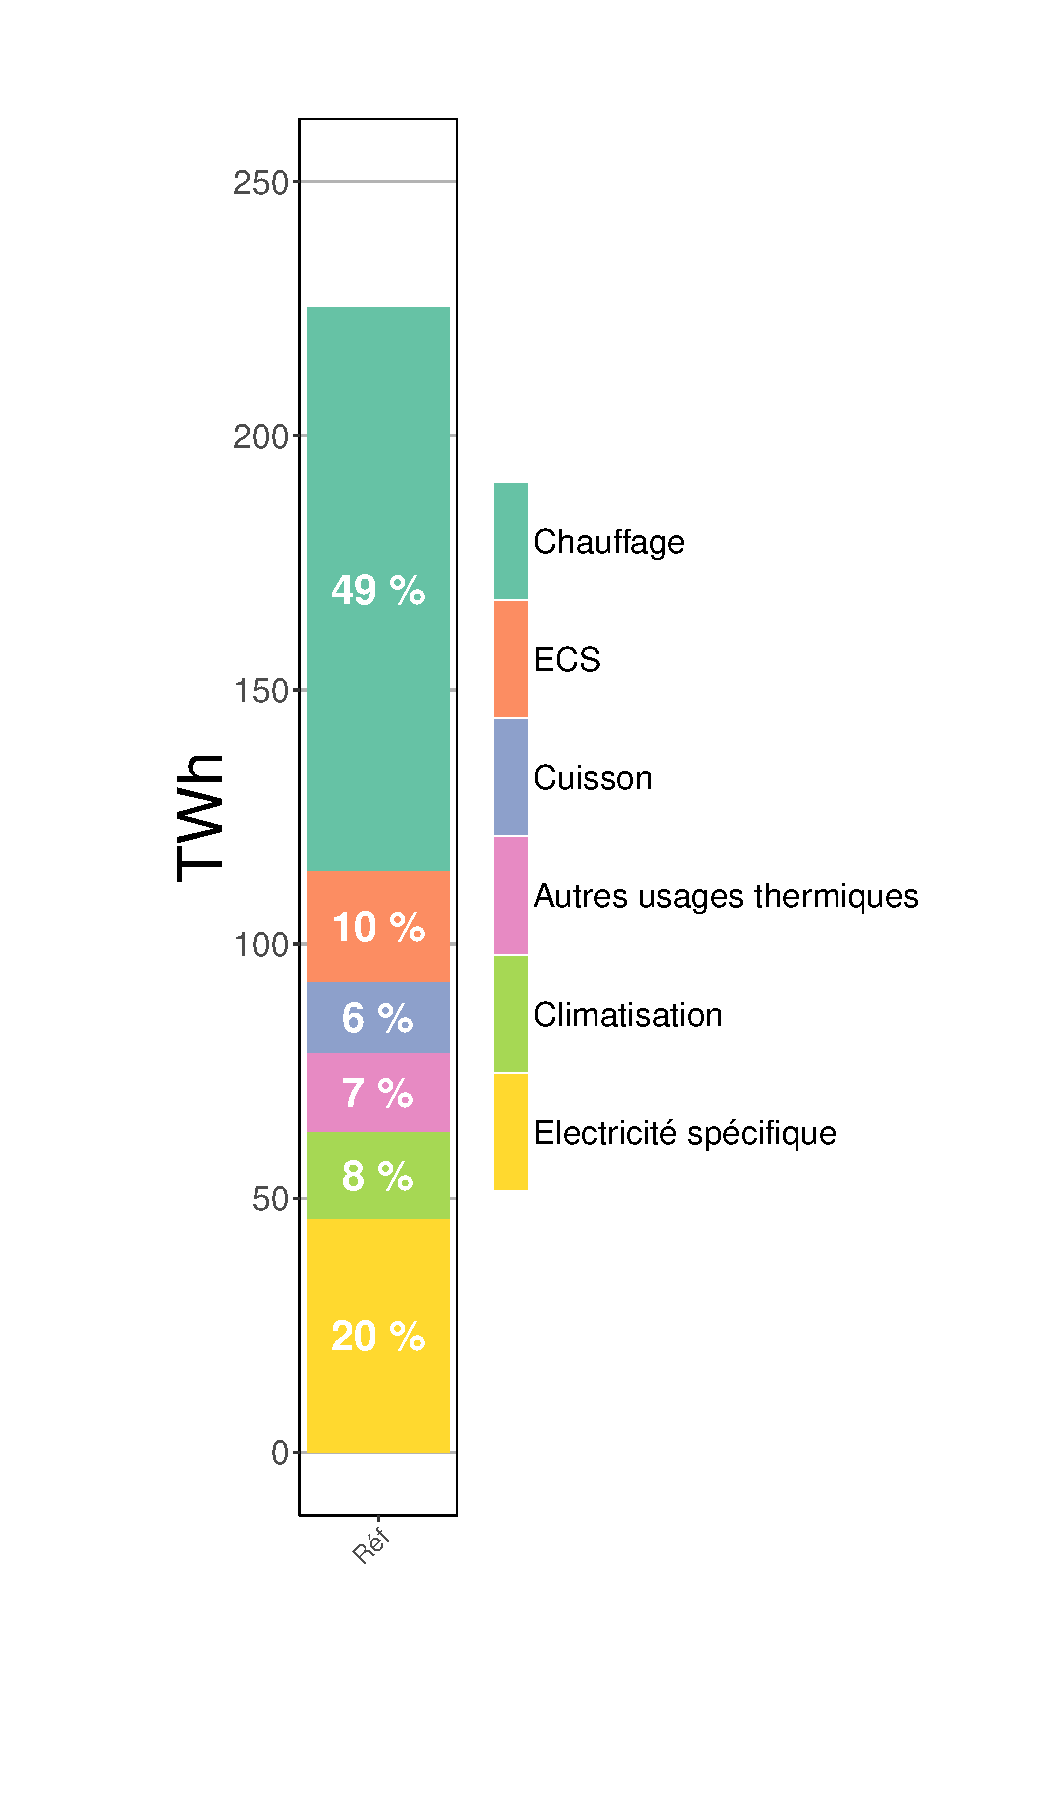
\includegraphics[width = 0.35\textwidth]{ConsoUsage2010} 
\end{tabular}
\end{figure}


\newpage 
\clearpage

\cleardoublepage

\thispagestyle{partie}
\cadreblanc{Partie 2}{Dynamique et calibration du modèle}{Résumé Partie}

\textbf{TODO INTRO COURTE}

\newpage
\pagestyle{fancy}

\invisiblesection{Dynamique et calibration du modèle}\label{sec:marker3}

\markboth{Partie 2 : Dynamique et calibration du modèle}{}

\subsection{Evaluation des potentiels d'économie d'énergie et coûts de mise en œuvre}

La caractérisation physique du parc par branche d’activité et bâtiment type présentée plus haut rend possible l’étude fine de gisements d’économies d’énergie, en simulant pour chacun des bâtiments types l’application de gestes de rénovation thermique. Pour modéliser les gisements d'économies d'énergie, il est nécessaire de disposer de données : 

\begin{enumerate}
	\item Sur les gains en énergie liés aux gestes de rénovation qui donnent le potentiel d'économie d'énergie du geste 
	\item Sur les coûts du geste de rénovation qui permettent d'évaluer le gisement économiquement rentable
\end{enumerate}

Le gains absolus pour un même geste de rénovation ne seront pas les mêmes selon l'état initial du bâtiment sur lequel on il est appliqué. Il est donc nécessaire d'avoir sur l'état initial du parc et sur l'effet des gestes de rénovation par type de bâtiment et période de construction.   

Pour le chauffage, deux principales sources d'économie d'énergie sont modélisées : les changements de systèmes de chauffage ou les gestes de rénovation sur le bâti. 

Les coûts moyens des systèmes de chauffage (Sources : Bâtiprix, UFE, CGDD) sont présentés ci-dessous. Pour un bâtiment type de besoin unitaire $B_u$, le gain en consommation d'énergie  $C_e$lié à un changement de système de chauffage est calculé en utilisant les rendements de la table \ref{Rdtsyst}. 

\begin{eqnarray}
 C_e &= &B_u * ( \frac{1}{R_i} -  \frac{1}{R_f}) \\
\end{eqnarray}

où $R_i$ est le rendement du système initial et $R_f$ celui du système final. Si le changement de système implique un changement d'énergie, le gain sur la facture énergétique  $F_e$ s'exprime

\begin{eqnarray}
 F_e &= & B_u * ( \frac{1}{R_i} * p_i -  \frac{1}{R_f}* p_f)  
\end{eqnarray}
où $p_i$ est le prix de l'énergie du système initial et $p_f$ celui de l'énergie du système final.  


\begin{table}[h!]
\scriptsize
\caption{Coûts moyens des systèmes de chauffage dans le modèle}
\label{Coutsyst}
\begin{center}
\begin{tabular}{l|c|c}
\textbf{Système}	&	\textbf{Investissement } & \textbf{Maintenance } \\
									& \textbf{(euros par m²)} & \textbf{(\% du coût d'investissement)} \\
\\	\hline	\\	
Chaudière gaz	& 15 & 3,5\%\\	
Chaudière condensation gaz	& 18  & 3,5\%\\	
Chaudière fioul & 19  & 2\%\\	
Chaudière condensation fioul	& 24  & 2\%\\	
Electrique direct	& 10  & 0,1\%\\	
Electrique direct performant	& 12 & 0,1\% \\	
PAC	& 66 & 1,5\% \\	
PAC performant	&  80 & 1,5\%  \\	
Rooftop	& 39  &  1,5\% \\	
Rooftop performant	& 46 &  1,5\%  \\	
DRV	& 20 &  1,5\% \\	
DRV performant	& 24 &  1,5\% \\	
Tube radiant	& 10 & 0,1\%\\	
Tube radiant performant	& 12 & 0,1\%\\	
Cassette rayonnante	& 10& 0,1\% \\	
Cassette rayonnante performant	& 12 & 0,1\% \\	
Autre système centralisé (Bois)	& 31 & 2\% \\	
Autre système centralisé (Urbain) & 31  & 2\%\\	
Autre système centralisé performant (Bois)	& 37  & 2\%\\	
Autre système centralisé performant (Urbain)	& 37  & 2\%\\	
\hline	
\end{tabular}
\end{center}
\footnotesize{\textbf{ Les coûts affichés ici sont des coûts moyens qui peuvent varier sensiblement d'un bâtiment type à l'autre selon la puissance demandée et la taille du bâtiment. Sources : Bâtiprix, UFE, CGDD}}
\end{table}


Les gestes sur le bâti sont caractérisés par un ou plusieurs postes de l’enveloppe bâtie ciblés par la rénovation (toiture, parois opaques, vitrage ou plancher bas). Trois types de gestes sont modélisés : un geste sur les parois vitrées (geste FEN), un geste sur les parois vitrées et opaques  (geste FENMUR) et un geste sur l'ensemble de l'enveloppe bâtie (geste ENS). Pour chacun de ces types de gestes, deux niveaux d'exigence sont modélisés : un niveau modéré (MOD) correspondant aux exigences de la Réglementation thermique élément par élément et un geste performant (BBC) correspondant à un niveau d'exigence proche du label BBC rénovation. 
Le modèle intègre aussi un geste « Gestion Technique du Bâtiment » qui correspond à une meilleure gestion du confort intérieur et des systèmes. 
Les gestes de travaux portant sur l’enveloppe bâtie sont donc au nombre de sept. 

Les gains liés à ces gestes de rénovation sont estimées par des simulations thermiques dynamiques effectués sur le modèle du CEP. Pour chaque bâtiment type du parc et selon la période de construction, il a été simulé une mise en conformité des parois au niveau RT élément par élément et au niveau BBC. On calcule ensuite le besoin unitaire du bâtiment une fois ces modifications de parois effectuées. On obtient un gain  $G_e$ en \% du besoin unitaire initial du bâtiment. 

\begin{eqnarray}
 G_e &= & 1-\frac{B_{u,f}}{B_{u,i}} \\
\end{eqnarray}


Le coût des gestes est calculé à partir du coût unitaire par m² de paroi des matériaux d'isolation et des paramètres du bâtiment type (surfaces des parois concernées, hauteur, taux de vitrage, forme...). Les coûts utilisés incluent la main d’œuvre mais pas les travaux de finition. 

\textbf{ PARLER DU RECALAGE AVEC LA COURBE OPEN...?}

Les résultats de ces simulations sur les types de gestes considérés, leurs coûts et les gains moyens sur les consommations de chauffage sont décrites dans le tableau \ref{Coutsyst}. Ces chiffres correspondent à des valeurs moyennes sur l’ensemble d'une branche d'activité et peuvent être très variables selon le bâtiment du parc considéré. 

\begin{table}[h!]
\caption{Coûts et gains moyens des gestes de rénovation dans le modèle}
\label{Coutsyst}
\begin{center}
\begin{tabular}{l|l|c|c}
\textbf{Branche} & \textbf{Geste}	&	\textbf{Investissement } & \textbf{Gain } \\
									& & \textbf{(euros par m²)} & \textbf{(\% du besoin unitaire )} \\
									\hline \\
Bureaux Administration &ENS\_MOD   &85 & 63\%\\
Bureaux Administration &ENS\_BBC  &430 &83\%\\
Café Hôtel Restaurant &ENS\_MOD  &221 &25\%\\
Café Hôtel Restaurant& ENS\_BBC &1193 &80\%\\
Commerce& ENS\_MOD  &184 & 41\%\\
Commerce &ENS\_BBC  &388& 68\%\\
Enseignement Recherche &ENS\_MOD  &153 & 57\%\\
Enseignement Recherche &ENS\_BBC  &383 & 80\%\\
Habitat Communautaire &ENS\_MOD   &98 & 25\%\\
Habitat Communautaire &ENS\_BBC  &407 & 75\%\\
Santé Action Sociale &ENS\_MOD   &74 & 43\%\\
Santé Action Sociale &ENS\_BBC  &237 & 80\%\\
Sport Loisir Culture &ENS\_MOD  &144& 47\%\\
Sport Loisir Culture &ENS\_BBC  &384& 73\%\\
\hline	
\end{tabular}
\end{center}
\footnotesize{\textbf{ Les coûts et les gains affichés ici sont des coûts moyens qui peuvent varier sensiblement d'un bâtiment type à l'autre selon la puissance demandée et la taille du bâtiment}}
\end{table}
%
%\begin{table}[h!]
%\caption{Coûts et gains moyens des gestes de rénovation dans le modèle}
%\label{Coutsyst}
%\begin{center}
%\begin{tabular}{l|c|c}
%\textbf{Geste}	&	\textbf{Investissement } & \textbf{Gain } \\
									%& \textbf{(euros par m²)} & \textbf{(\% du besoin unitaire )} \\
%\\	\hline	\\	
%GTB & & \\	
%FENMOD & & \\	
%FENMUR\_MOD  & & \\	
%ENSMOD & & \\	
%FENBBC & & \\	
%FENMUR\_BBC & & \\	
%ENS\_BBC & & \\	
%\hline	
%\end{tabular}
%\end{center}
%\footnotesize{\textbf{ Les coûts et les gains affichés ici sont des coûts moyens qui peuvent varier sensiblement d'un bâtiment type à l'autre selon la puissance demandée et la taille du bâtiment}}
%\end{table}

%PB VALEURS MOYENNES DES COUTS POUR LES GESTES FEN ET FENMUR: 

Les amplitudes observées sur les gains et coûts sont le fait des bâtiments très différents composant le parc tertiaire, tant en terme de morphologie (petit restaurant rapide/hôpital) qu’en terme de paramètres d’occupation (foyer/gymnase). Ainsi, ces différences entraînent des impacts de mise en œuvre des gestes sur le bâti très variables d’un bâtiment à un autre.
+ AJOUTER UN EXEMPLE

\subsubsection{Coûts des systèmes ECS, éclairage et climatisation}

\textbf{TODO A COMPLETER :  coûts fixes par m²}

\newpage 
\clearpage
\subsection{Dynamique du parc}

La dynamique du modèle se base à la fois sur une évolution mécanique du parc et une dynamique interne de rénovation du bâti et des systèmes de production. Ainsi, chaque année, le parc de bâtiments tertiaires évolue quantitativement et qualitativement.

\begin{figure}[h!]
\centering
\caption{Dynamique du parc dans le modèle }\label{schema_dyn}

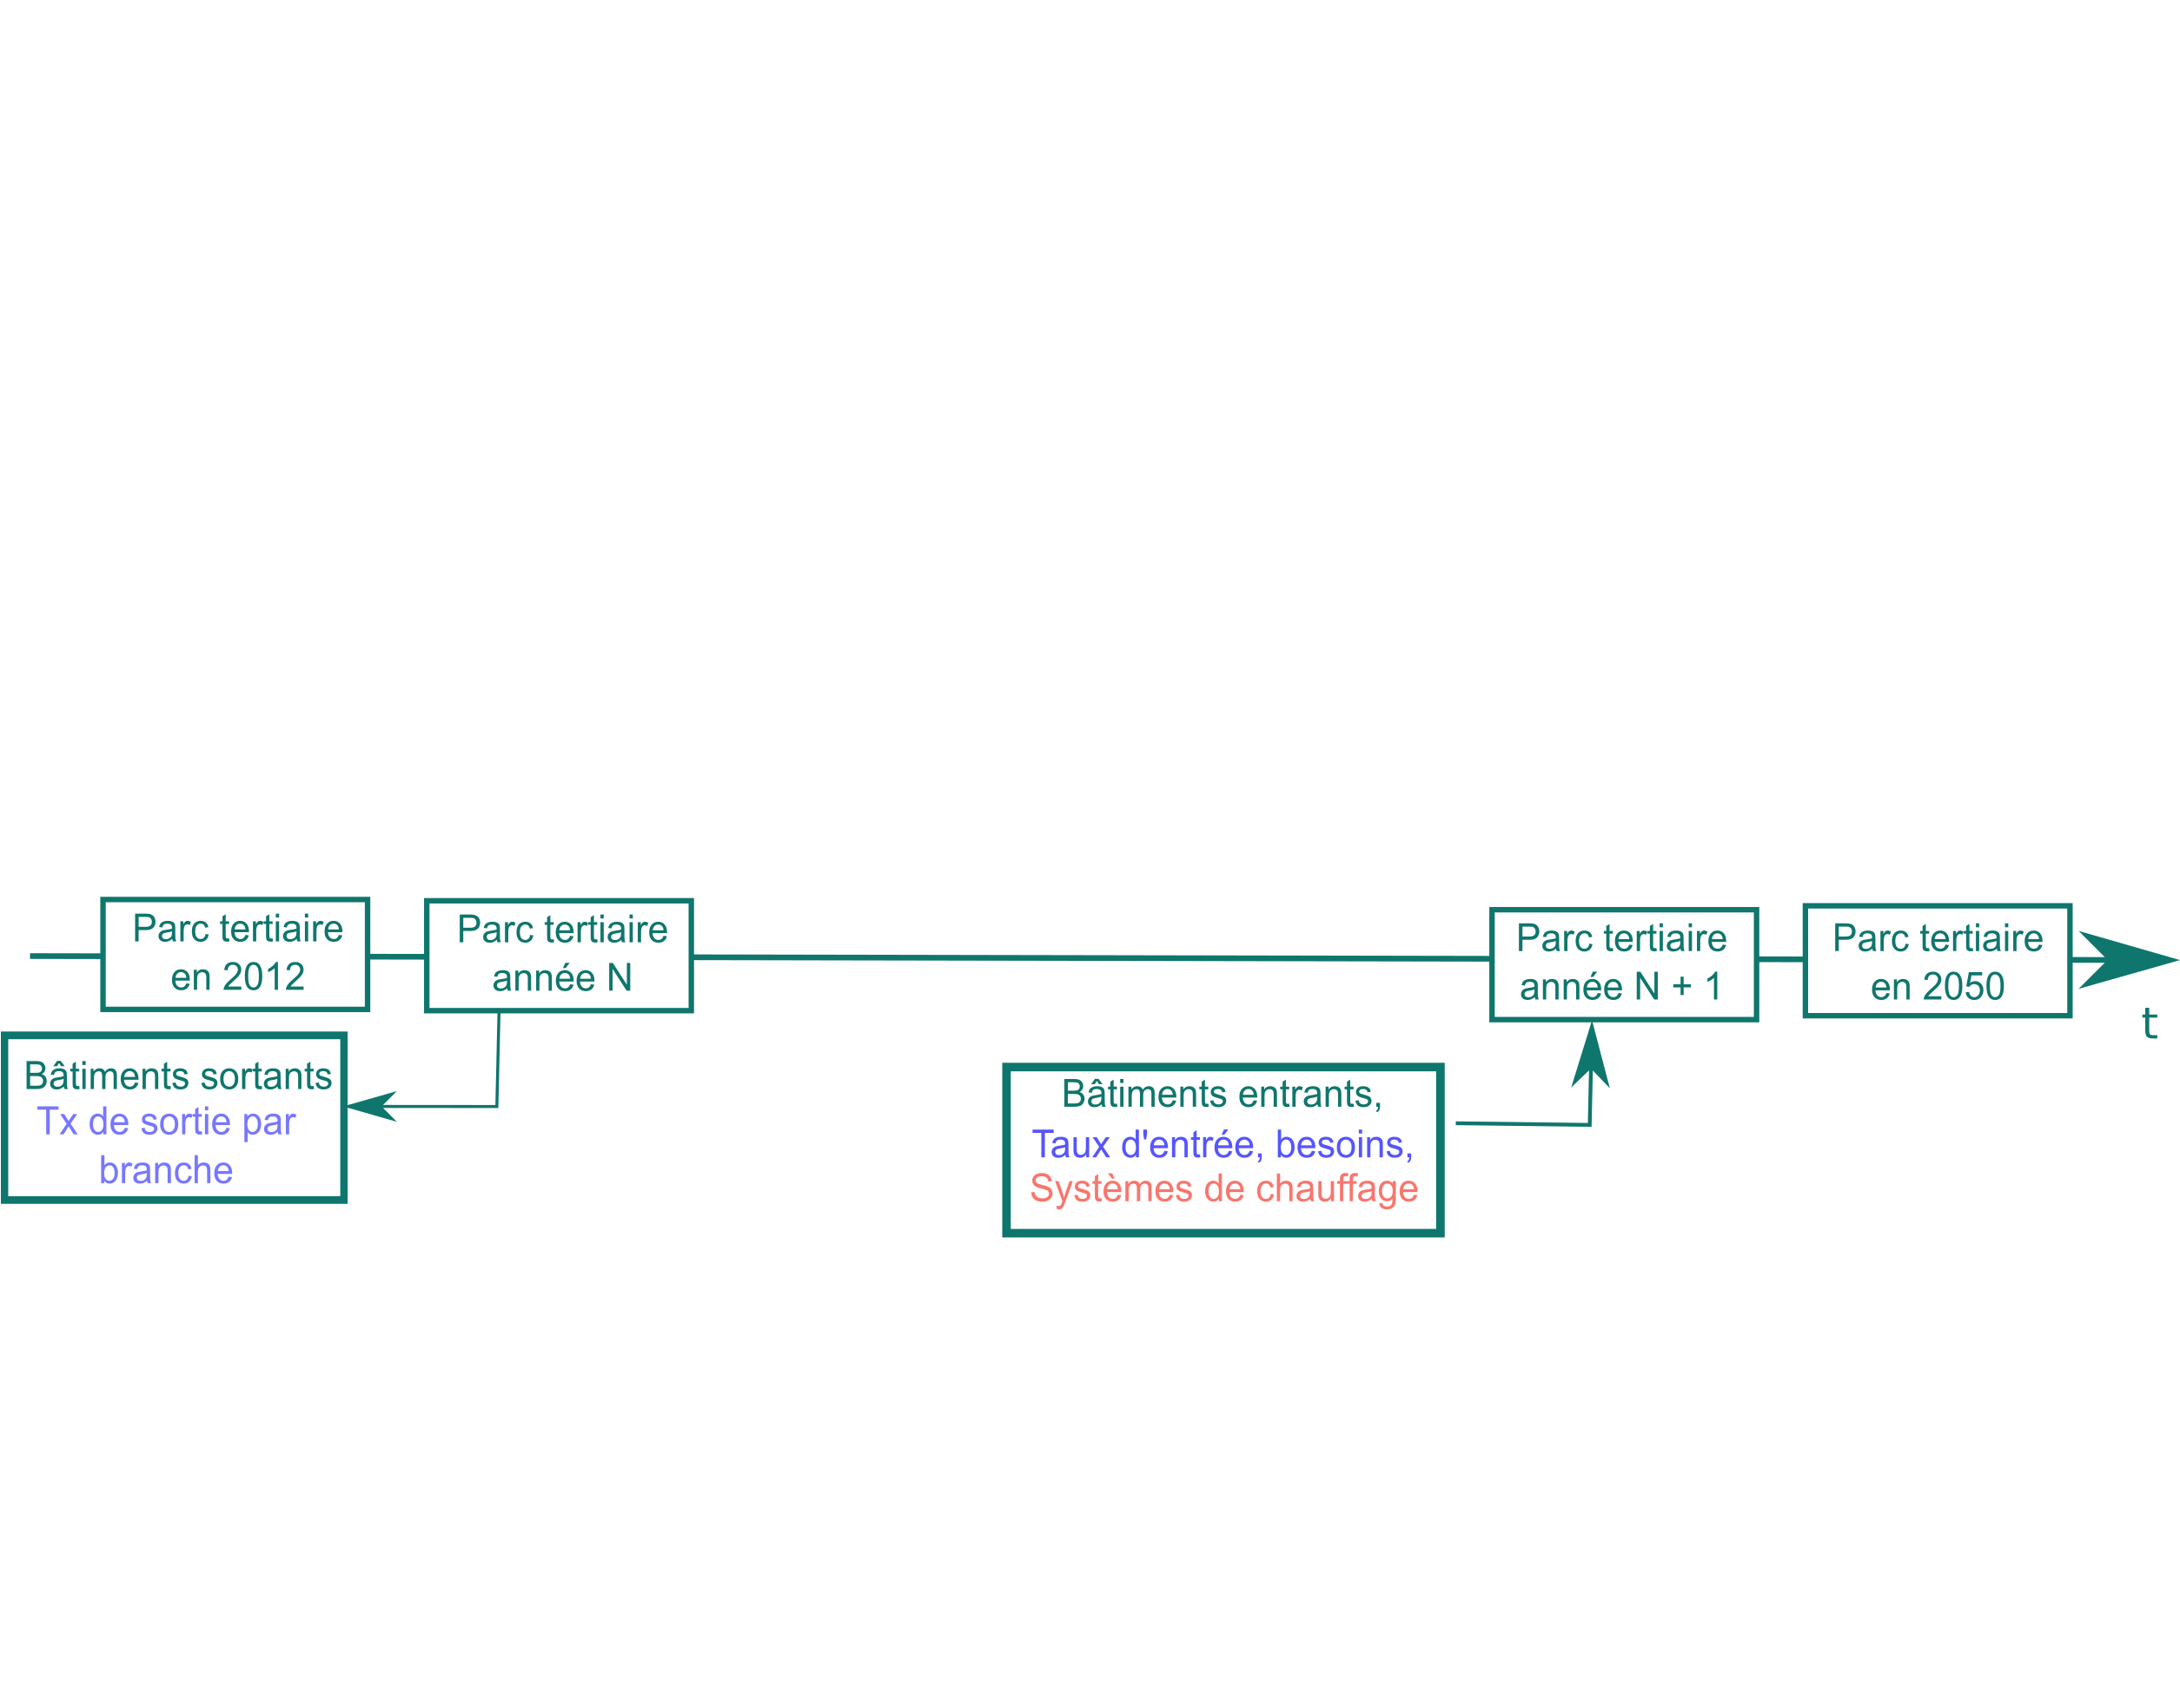
\includegraphics[width = 0.7\textwidth]{schema_dyn}  

\end{figure}

Chaque année des bâtiments « entrent » (construction neuve, changement d’usage) et « sortent » (démolition, changement d’usage) du parc tertiaire. Ces rythmes conditionnent l’évolution du parc tertiaire d’une année sur l’autre.
\begin{itemize}

\item Sorties : Les surfaces sortantes sont issues du produit des taux de sortie du parc avec les surfaces existantes à l’année n-1. 
\item Entrées : Les surfaces entrantes dans le parc sont issues du produit des taux d’entrée dans le parc avec les surfaces existantes à l’année n-1 (hors surfaces sortantes). 
\end{itemize}


Les taux annuels surfaciques d’entrée et de sortie du parc par branche d'activité sont paramétrables de manière exogène selon les scénarios d'évolution du parc envisagés. 

Les performances thermiques des bâtiments entrants sont aussi paramétrées de manière exogène par bâtiment-type et usage. On Définit par usage les besoins unitaires en kwh par m² pour chaque de bâtiment. Il est possible de faire évoluer les performance du bâti neuf dans le temps de manière à simuler dés évolutions de réglementations thermiques.

Les parts de marché des énergies des bâtiments neufs pour les usages de cuisson, ECS et autres sont paramétrés de manière exogène. En l'absence de données plus documentées, elles ont été considérées égales à celles du parc de l’état initial. 
 
Les parts de marché des énergies pour le chauffage des bâtiments entrants sont déterminées de manière endogène dans le modèle chaque année. Elles résultent d’un calcul de rentabilité des systèmes en fonction des prix des énergies, du coût d’investissement et du coût de maintenance du système installé, des besoins unitaires du segment de parc entrant considéré et du rendement du système installé. Le calcul des parts de marché des énergies pour le chauffage des bâtiments entrants est similaire à celui effectué pour le parc existant. Il est détaillé dans la section suivante. 



\subsection{Rénovation du parc existant }

A l’année n, le modèle évalue les possibilités de gestes de travaux qu’il est envisageable de mener sur chacun des segments constituant le parc tertiaire. 
Pour envisager une rénovation, le modèle raisonne segment de parc par segment de parc. Un segment se caractérise par :
\begin{itemize}
\item une branche d’activité
\item une sous-branche d’activité
\item un bâtiment-type
\item un type d’occupant
\item une période de construction
\item un système de chauffage
\item un système de froid
\item une énergie de chauffage
\end{itemize} 

Il est considéré dans le modèle de simulation que les rénovations thermiques des bâtiments n’ont d’incidence que sur les consommations de chauffage, d’auxiliaires et de ventilation. Seules les rénovations thermiques d’exigence BBC  touchant l’ensemble du bâtiment (geste ENS\_BBC) ont une incidence sur les consommations d’eau chaude sanitaire et d’éclairage.

Ainsi, deux mécaniques d’évolution des consommations énergétiques sont modélisés selon l’usage considéré
\begin{itemize}

 \item Evolution des consommations conditionnée par une fonction de passage à l’acte de rénovation et par les rythmes de vie des matériaux de construction des enveloppes bâties (usages concernés : chauffage, ventilation, auxiliaires, et dans le cas d’une rénovation de l’ensemble du bâti par un geste d’exigence BBC : éclairage et ECS).

\item Evolution des consommations conditionnée par les rythmes de vie des systèmes ainsi que par des paramètres exogènes (usages concernés : cuisson, bureautique, process, climatisation, froid alimentaire, usage autres et éclairage et ECS dans le cas où aucune rénovation BBC sur l’ensemble du bâti n’est menée).
\end{itemize} 

La fonction de passage à l’acte est centrale dans le modèle de simulation. Elle a pour but de déterminer chaque année pour tous les segments de parc, les parts de marché de chacun des gestes de travaux pouvant être menés. Il est à noter qu’un geste de travaux est constitué d’une action sur l’enveloppe du bâti et/ou sur les systèmes. Ne réaliser aucune rénovation ou changement de système est comptabilisé comme une action (Geste \og~Ne rien faire~\fg).La gestion technique du bâtiment (GTB) est prise en compte comme une action sur les systèmes.


\begin{figure}[h!]
\centering
\caption{Dynamique de rénovation dans le modèle }\label{schema_renov}

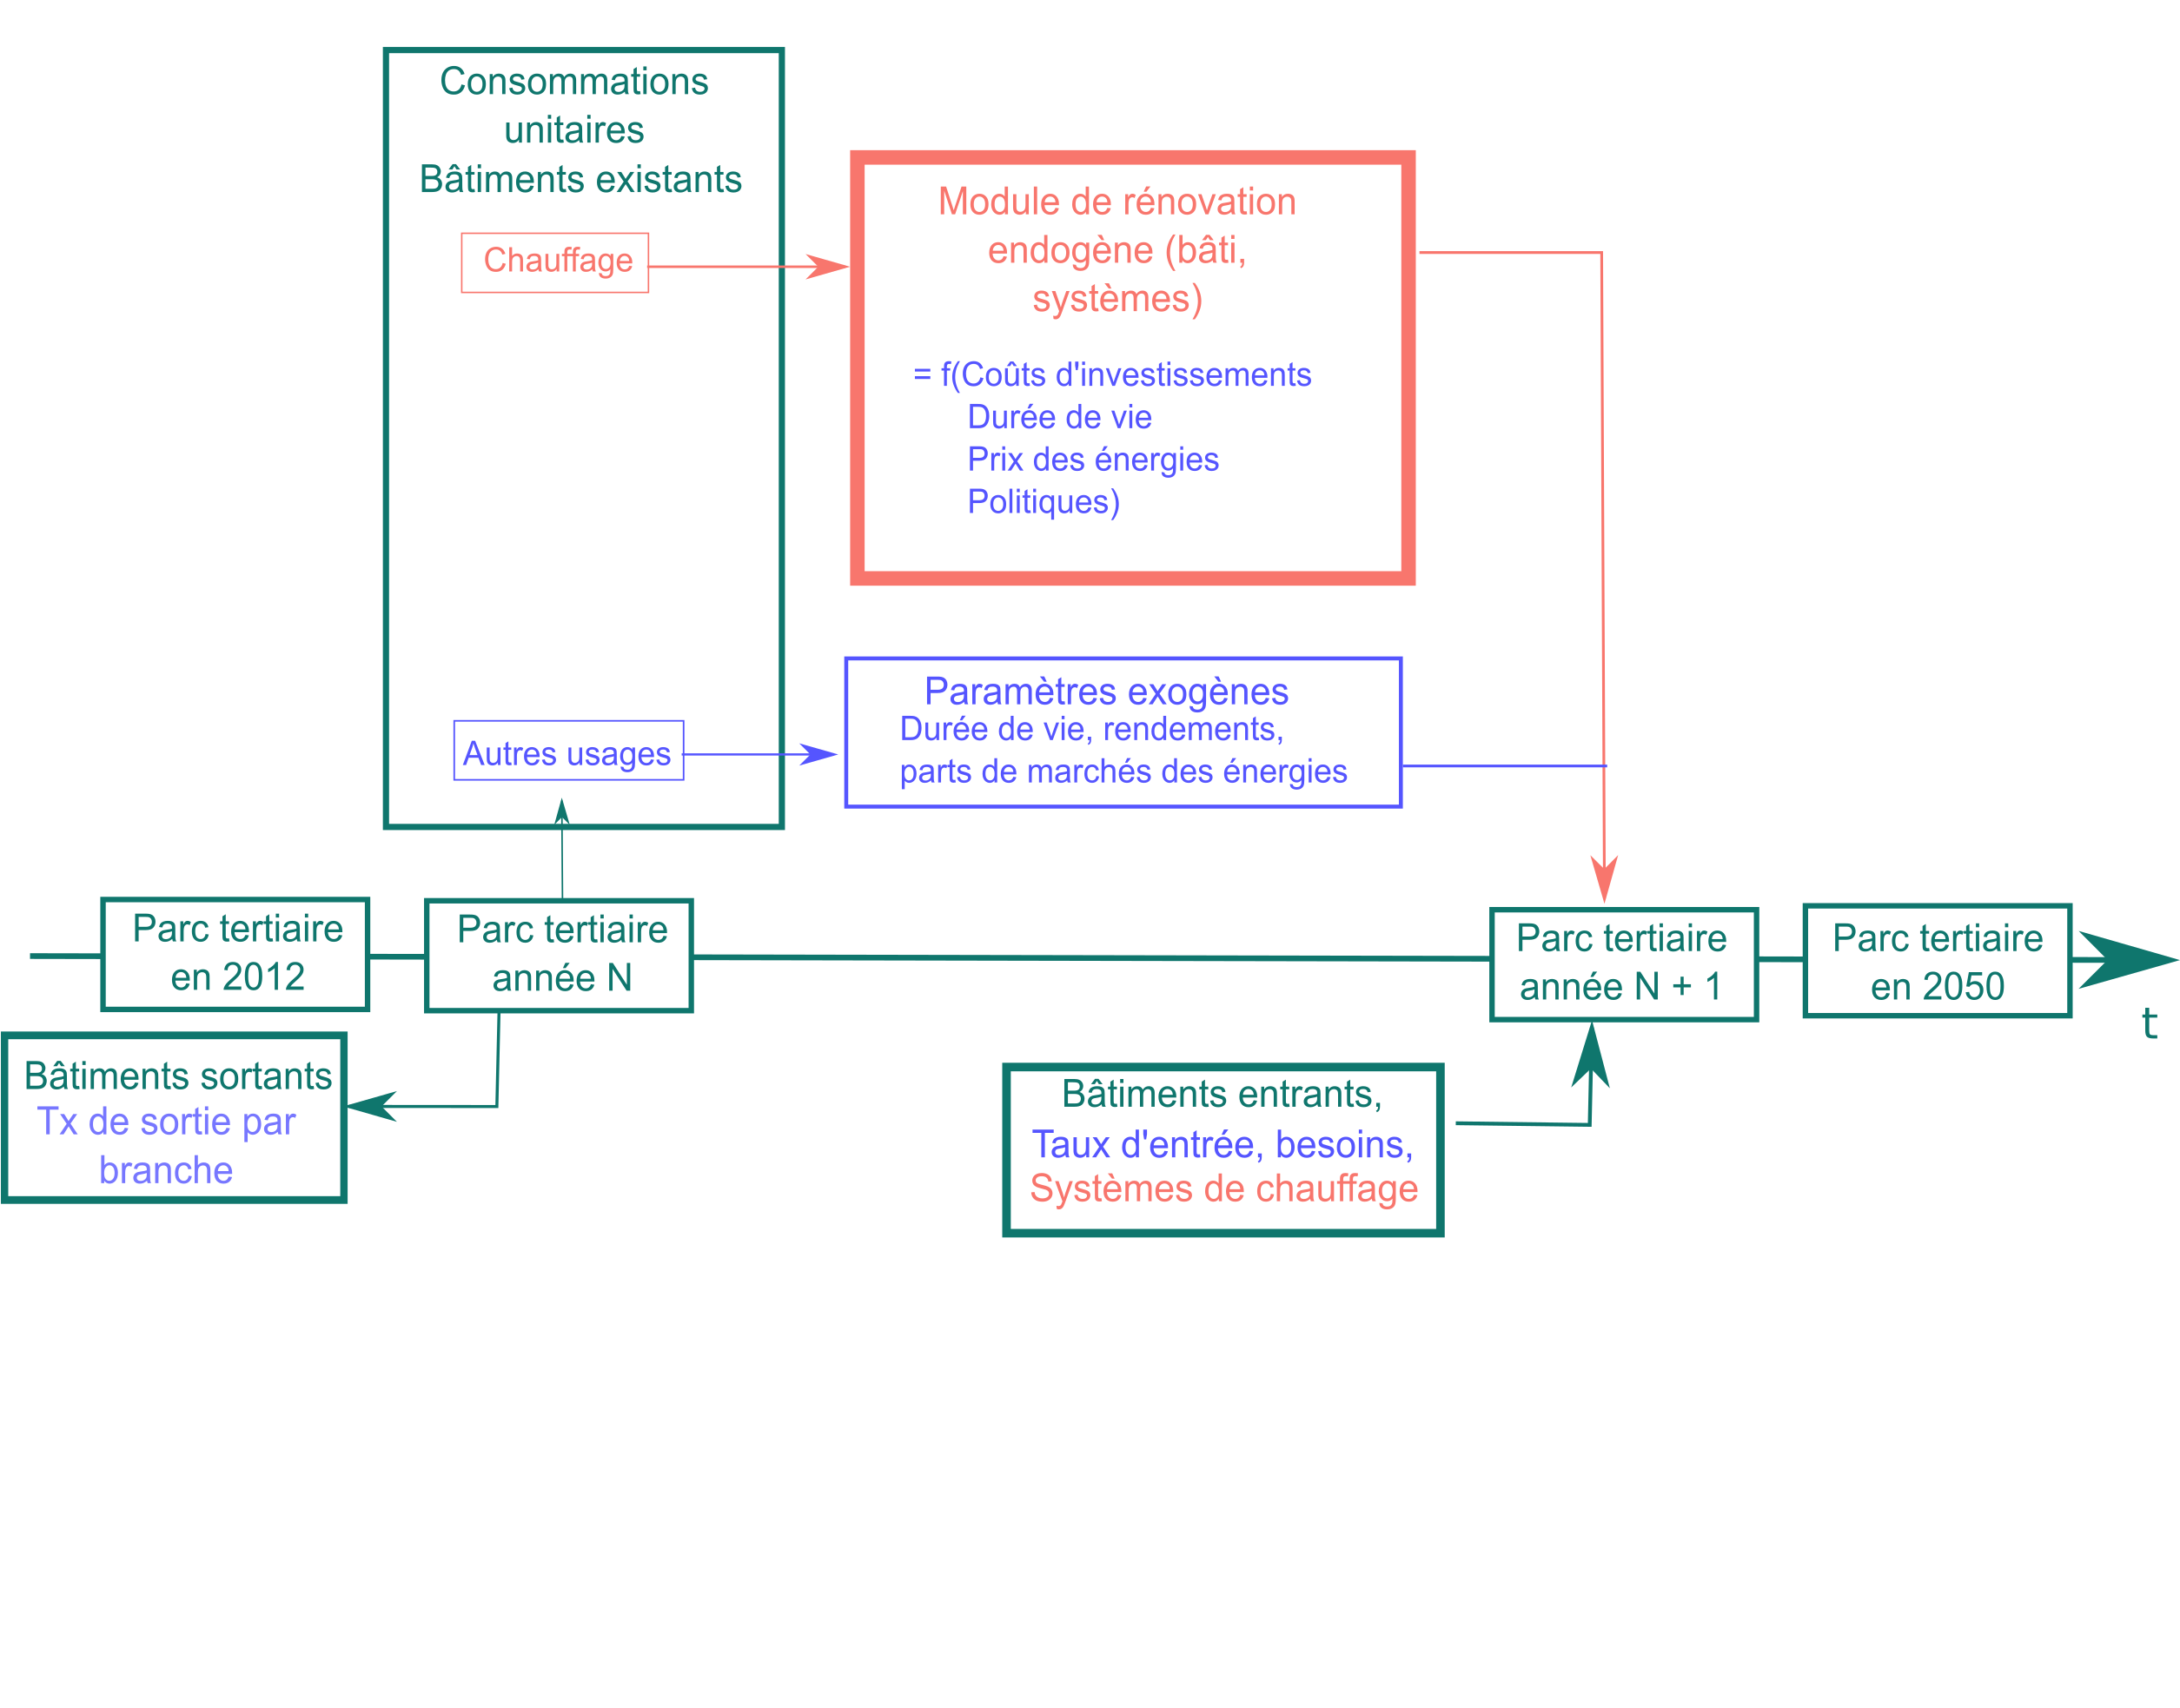
\includegraphics[width = 0.7\textwidth]{schema_renov}  

\end{figure}


La méthode de détermination des parts de marché se décompose en trois phases :

\begin{enumerate}
	\item Détermination de l’ensemble des possibilités de travaux
	\item Description des modes de financement envisageables
	\item Calcul des parts de marché de chacune des combinaisons travaux/financement
\end{enumerate}

\subsubsection{Détermination de l’ensemble des possibilités de travaux}

Chaque année, le modèle évalue les travaux qu'il est possible de mener sur chaque segment et pour chaque combinaison geste sur le bâti - changement de système de chauffage. Il est important de noter qu’un changement de système n’est envisagé que lorsque le système déjà en place arrive au terme de sa durée de vie. Tous les types de systèmes de chauffage ne peuvent pas être installés sur tous les bâtiments. Les systèmes DRV sont par exemple installables seulement dans les bureaux ou les équipements de collectifs de sport et culture. Les cassettes rayonnantes et les tube radiant sont également plus spécifiques aux équipements de loisir et sport.  


Le modèle intègre également la possibilité de paramétrer des outils réglementaires : 
\begin{itemize}
\item Niveau d’exigence minimale admissible lors d’une rénovation
\item	Obligation de travaux, exprimée en part du parc touché selon le type d’occupant. La nature du geste de travaux imposé est également renseignée par l’utilisateur.
\item	Décret d’application de la loi Grenelle. Celui-ci fixe une part de la surface touchée par branche et type d’occupant. La nature du geste imposé est déterminée par le modèle en fonction de paramètres définis par l’utilisateur tels qu’un temps de retour sur investissement maximal, un coût maximal des travaux, un gain minimal attendu sur les consommations d’énergie primaire des usages RT, ainsi que les années d’entrée en vigueur et de fin du dispositif. Tous les gestes envisagés sur le segment de parc sont testés, et seuls ceux correspondant aux propriétés du décret sont imposés dans une proportion homogène sur les années d’existence de celui-ci.
\item	Obligation de fermeture des meubles frigorifiques pour les grandes surfaces commerciales.
\end{itemize}

Les réglementations en vigueur à l’année en cours ont une influence sur les possibilités de gestes de travaux en excluant certains gestes (s’ils ne respectent pas l’exigence minimale).

A l'issue de cette étape, on obtient une liste de gestes réalisables par segment.

\subsubsection{Description des modes de financement envisageables}

Le modèle de simulation offre la possibilité à l’utilisateur de décrire les dispositifs incitatifs mobilisables à l’année n. Ceux-ci sont de trois types : 

\begin{itemize} 
\item Les aides (certificats d’économies d’énergie)
\item Les prêts à taux bonifié et 
\item Les prêts bancaires classiques
\end{itemize}

Pour chacun des gestes de travaux réalisable, par segment de parc, on simule toutes les combinaisons aides/prêts bancaires (bonifié et/ou classique)selon le contexte à l’année n (prix des énergies, évolution des coûts d'investissement). Les combinaisons ou modes de financement sont alors caractérisés par la part du financement pris en charge par les aides et prêts bonifiés ainsi que par l’importance du reste à charge que devra financer le maître d’ouvrage par un recours à un prêt bancaire classique.
A chaque segment de parc et geste de travaux considérés sont donc associées plusieurs solutions de financement différentes caractérisées par : 

\begin{itemize} 
\item Un montant de l’investissement pris en charge par les aides et les prêts bonifiés
\item Un reste à charge finançable par des prêts bancaires classiques
\item Un montant des frais bancaires liés au financement du reste à charge
\end{itemize}


%Afin de décrire les modes de financement envisageables, plusieurs indicateurs seront calculés lors de cette étape par geste de travaux :
%•	Coût d’investissement actualisé sur la durée de vie des technologies/matériaux nécessaires à la mise en œuvre du geste
%•	Temps de retour sur investissement actualisé
%•	Coûts intangibles associés aux gestes de travaux

\subsubsection{Évaluation des parts de marché des combinaisons geste de travaux/mode de financement}

Afin de hiérarchiser les combinaisons geste de travaux/mode de financement, on calcule pour chacune d'entre elles un coût global de mise en œuvre des rénovations. Celui-ci permettra par la suite de calculer les probabilités de réalisation des gestes.

Le coût global ($CG$) est égal au coût d’investissement global ($CINV$) auquel s’ajoute la somme des charges énergétiques annuelles ($CE$) et des annuités de remboursement des prêts contractés (A) actualisés au taux $a$ sur la durée de vie des équipements ($DV$). 

Le taux d’actualisation est paramétrable selon la branche, l’occupant et le statut d’occupation des locaux (propriétaire/occupant). Par défaut, iles fixé à 4\% pour un propriétaire/occupant public et à 7\% pour un propriétaire/occupant privé. 

\begin{eqnarray}
 CG &= & CINV + \sum_{t = 1}^{DV} \frac{(CE + A)}{(1+a)^t}  \\
\end{eqnarray}

Afin de prendre en compte toutes les composantes de l’investissement, le coût d’investissement global est calculé comme suit :

\begin{eqnarray}
 CINV &= & CT + CTA - SUB - FIN  \\
\end{eqnarray}

Où :
\begin{itemize}
\item $CT$ est le coût des travaux de rénovations du bâti et des systèmes de chauffage installés
\item $CTA$ : le coût des travaux d’aménagements à réaliser lors d’un changement de solution de chauffage (par exemple les coûts de plomberie engendrés par le remplacement de convecteurs par une chaudière centralisée)
\item $SUB$ : les financements obtenus par des aides mais sans les prêts bancaires
\item $FIN$ : le capital emprunté à un taux $i$ sur une durée $DF$. 
\end{itemize}

A sont les annuités de remboursement du prêt avec 

\begin{eqnarray}
 A &= & \frac{FIN} {\sum_{t = 1}^{DF} \frac{1}{(1+i)^t} }  \\
\end{eqnarray}

Cette décomposition permet de prendre en compte les temps distincts de durée de vie des équipements et des temps de remboursement des prêts contractés. Le coût global ($CG$) se calcule donc sur la durée de vie du geste (DV) tandis que les annuités de remboursement du prêt (FBA) se calculent sur la durée de remboursement du prêt DF qui doit rester inférieure ou égale à DV. 

Enfin, les charges énergétiques ($CE$) sont calculées chaque année comme suit :

si le type d’énergie de chauffage ne change pas

\begin{eqnarray}
	CE &= & (p_i  \frac{B_{u,i}}{R_f}(1-G_e) + CM)S \\
 CE &= & p_i  \frac{B_{u,i}}{R_f}(1-G_e) + CM   \\
\end{eqnarray}

si l’énergie de chauffage est modifiée

\begin{eqnarray}
 CE &= & p_f \frac{B_{u,i}}{R_f}(1-G_e) + CM   \\
\end{eqnarray}


Où :
\begin{itemize}
\item $S$ est la surface moyenne du bâtiment du segment
\item $p_i$ est le prix de l’énergie pour la technologie initiale à l’année de simulation,  $p_f$ le prix de la nouvelle énergie de chauffage à l’année de simulation si il y a changement d'énergie. Il est important de noter que les agents sont considérés comme «myope» dans le modèle. Le prix utilisé pour le calcul du coût global est fixe dans le temps et correspond à celui de l’année d’investissement. 
\item $R_f$ est le rendement du nouveau système de chauffage installé.
\item $B_{u,i}$ le besoin unitaire de chauffage pour le bâtiment avant les travaux, $G_e$ est le gain énergétique en \% du besoin unitaire induit par le geste de rénovation du bâti.  
\item $CM$ est le coût de maintenance unitaire annuel du système de chauffage (fixe dans le temps). 
\end{itemize}

Cette évaluation du coût global a l’avantage de quantifier le coût d’une non-intervention sur le bâti ($G_e = 0$) ou les systèmes ($R_f = R_i$).

Sur la base du coût global calculé précédemment, pour chaque combinaison geste de travaux/mode de financement, la probabilité de réalisation est égale à :

\begin{eqnarray}
PM_g & = & \frac{CG_g^{-\nu}}{\sum_g CG_g^{-\nu}}
\end{eqnarray}


Où :
\begin{itemize}
\item$g$ est l’indice des différentes combinaisons geste de travaux/mode de financement existant sur le segment
\item $PM_g$ est la probabilité de réalisation de la combinaison geste de travaux/mode de financement
\item $CG_g$ est le coût global de la combinaison geste de travaux/mode de financement $g$
\item $\nu$ est un paramètre d’hétérogénéité du marché. Il s’agit d’une valeur positive impliquant une probabilité non nulle pour chaque combinaison et rendant compte de la diversité des situations existantes et des gestes de rénovation choisis. Cette valeur est directement paramétrable par l’utilisateur. Par défaut ce paramètre sera fixé à 8, à l’instar de la valeur retenue par le CIRED pour son évaluation récente des politiques de réduction de la demande d’énergie du parc de logements \citep{Giraudet_etal2018}.
\end{itemize}

Ainsi, plus le coût global d’une option sera élevé, plus la probabilité de passage à l’acte sera faible. Cette formulation de la probabilité de passage à l’acte permet d’éviter qu'un système de chauffage ou un geste de rénovation prenne l'intégralité des parts de marché ce qui ne correspond pas à la réalité. 

Dans le cas où une ou plusieurs réglementations sont en vigueur durant l’année en cours, les gestes imposés (directement dans le cas d’une obligation de travaux ou bien choisie par le modèle en fonction de critères pour le décret d'obligation) se voient directement attribuer une part de marché correspondant à la part du parc touché par le ou les dispositifs. L’évaluation des parts de marché des autres gestes est alors réalisée sur la part du segment non concernée par la ou les réglementations.

\subsection{Dynamique pour les autres usages}

\textbf{TODO EXOGENE BLABLA}

Détail climatisation

Enfin, une rénovation de l’enveloppe bâtie (quel que soit le geste de travaux considéré) entraîne d’une part l’apparition d’un effet rebond, augmentant les consommations d’énergie de chauffage, et le remplacement du système de ventilation par un système double flux à récupération de chaleur, une redéfinition des systèmes d’éclairage et d’ECS. 

Il est à noter que les consommations d’auxiliaires de chauffage évoluent proportionnellement à celles de l’usage de chauffage. 


\subsection{Évolution des consommations et des émissions}

Sur la base des parts de marché calculées précédemment, les consommations énergétiques et les émissions de gaz à effet de serre sont recalculées pour chaque nouvelle année de simulation. Les consommations obtenues à l’année n+1 sont fonction des travaux réalisés (ou non) sur l’enveloppe bâtie et du remplacement ou non du système de chauffage. 

Les émissions de gaz à effet de serre sont calculées à partir des consommations d’énergie finale et des taux d’émissions définis pour la période en cours par l’utilisateur. Les taux d'émissions utilisés par énergie sont décrits dans la partie suivante sur les scénarios simulés. 


\begin{figure}[h!]
\centering
\caption{Sorties du modèle }\label{schema_final}

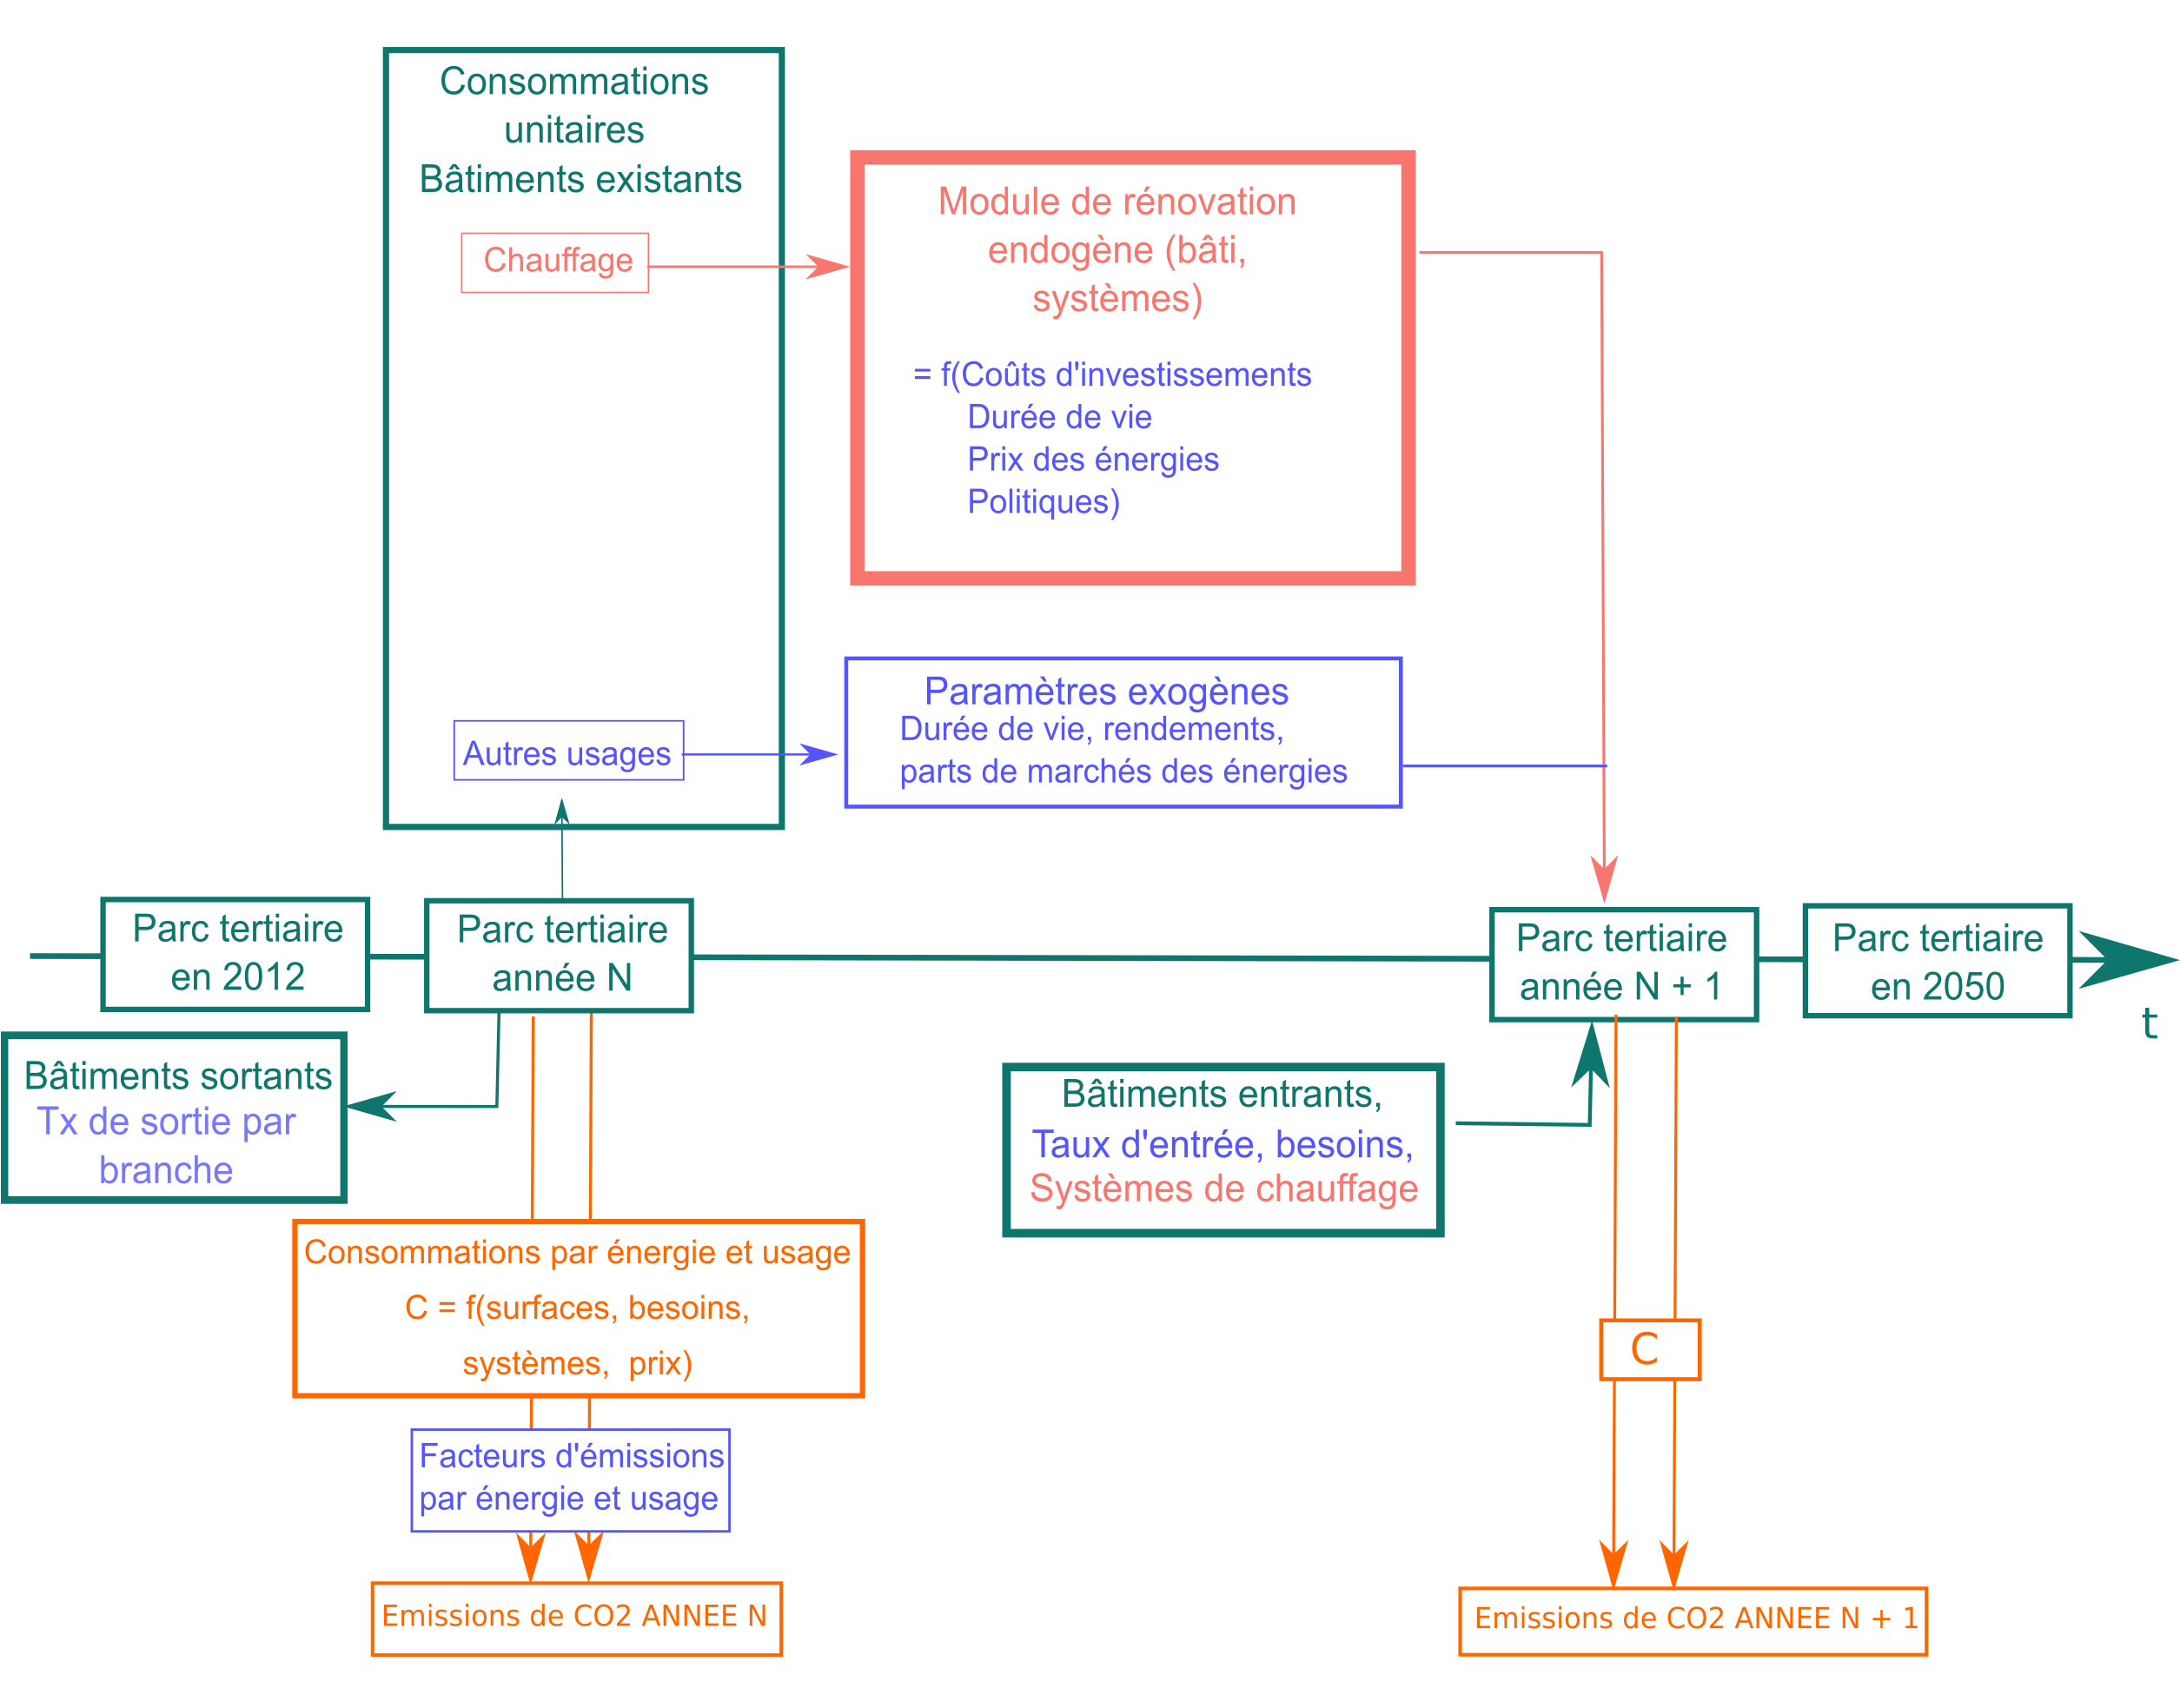
\includegraphics[width = 0.7\textwidth]{schema_final}  

\end{figure}

\subsection{Calibration initiale du modèle}

Peu de données sont disponibles sur le niveau des investissements dans la rénovation énergétique des bâtiments dans le tertiaire. Pour calibrer le rythme initial de rénovation dans le modèle (gestes sur le bâti et renouvellement des systèmes de chauffage), nous utilisons deux sources de données principales : 

\begin{itemize}
\item Deux études réalisées par le bureau d'études CODA Strategies qui fournissent des montants pour les marchés de la rénovation dans le secteur tertiaire par type de geste (ouvrants, façade, isolation, gestion technique du bâtiment, climatisation, chauffage et ventilation), par type de système de chauffage installé et par branche du secteur tertiaire (\cite{CODA_2015}, \cite{CODA_2016}).
\item L'évolution des surfaces chauffées par énergie et des consommations nationales des bâtiments tertiaires par usage et énergie du CEREN entre 2010 et 2015
\end{itemize}

Les parts de marché initiale des changements de système dans l’existant pour chaque segment du parc sont également calibrées pour tenir compte des évolutions récentes observées avec notamment une baisse marquée de la part de marché du fioul dans les consommations et une croissance de la part de marché de l’électricité et  la pénétration dans le parc des systèmes performants (ex : chaudière condensation, systèmes DRV, Rooftop et PAC).

\subsubsection{Rythme initial de rénovation du bâti par branche}

CODA Strategies estime des marchés de la rénovation tertiaire de 10.2 milliards d'euros en 2014. Les gestes de rénovation sur l'enveloppe des bâtiments (ITI, ITE, ouvrants, façades) ne représentent néanmoins seulement environ 12~\% du marché de la rénovation soit 1.2 milliards d'euros. 30~\% de ces investissements sont réalisés dans les bureaux, 17~\% dans les bâtiments d'enseignement et 15~\% dans les commerces.  Les investissements dans la gestion technique des bâtiment ne représentent que 100 millions d'euros par an. 

En appliquant les fonctions de passage à l'acte aux coûts d'investissements des gestes de rénovation présentés plus, nous obtenons un taux de rénovation du parc très important, supérieur aux estimations des études CODA sur le tertiaire. Cet écart peut provenir d'une sous-estimation des coûts de rénovation du fait de de plusieurs facteurs :  

\begin{itemize}
\item La réticence à installer une technologie nouvelle 
\item La perte d’activité occasionnée par des travaux en site occupé
\item L’apprentissage lié à l’usage de nouvelles installations
\end{itemize}

Ces facteurs entraînent des coûts pour le propriétaire des bâtiments qui ne sont pas pris en compte dans les coûts observés dans les bases de données. On parle généralement de coûts non observés ou \og~coût intangibles~\fg.  

Pour calibrer le rythme initial de rénovation par branche dans le modèle sur les données estimées par CODA Strategies, nous introduisons un paramètre ($\lambda_b$) qui permet de contrôler le nombre de rénovation sur le bâti de la branche $b$ dans le modèle. Ce paramètre est inférieur à 1et est utilisé comme facteur multiplicatif pour le coût global du geste \og~Ne rien faire~\fg, geste qui consiste à ne réaliser aucune rénovation ou changement de système est comptabilisé comme une action (Geste \og~Ne rien faire~\fg). Ainsi, plus $\lambda_b$ est petit, plus le coût global du geste \og~Ne rien faire~\fg est petit et plus il est intéressant de ne pas réaliser de geste de rénovation. Les parts de marchés de l'ensemble des autres gestes sur le bâti vont donc diminuer lorsque $\lambda_b$ diminue. L'intérêt d'utiliser un seul paramètre est que les gestes les plus rentables vont tout de même conserver une part de marché plus grande (bien qu'inférieure au calcul avant introduction de $\lambda_b$) que les gestes moins rentables.  

Pour un bâtiment appartenant à la branche $b$, le coût global \og~modifié~\fg pour le geste \og~Ne rien faire~\fg s'exprime donc :
 
\begin{eqnarray}
 CG_b &= &  \lambda_b * \sum_{t = 1}^{DV} \frac{(CE_b)}{(1+a)^t}  \\
\end{eqnarray}

La valeur du paramètre $\lambda_b$ pour chaque branche est fixée de manière à reproduire au mieux les montants des marchés de rénovations pour les gestes sur l'enveloppe du bâtiment et la gestion technique du bâtiment observés dans l'étude CODA sur les marchés de la rénovation. La figure \ref{Comparaison_Renovbati_CODA} compare les montants investis obtenus dans le modèle (montants moyens simulés sur les années 2015 à 2020) avec les montants estimés en 2014 par CODA Strategies. Les montants investis par branche dépendent de nombreux paramètres dans le modèle, il est donc difficile d'ajuster parfaitement aux  

\begin{figure}[h!]
\centering
\caption{Calibration des montants investis dans la rénovation de l'enveloppe des bâtiments et la GTB}\label{Comparaison_Renovbati_CODA}
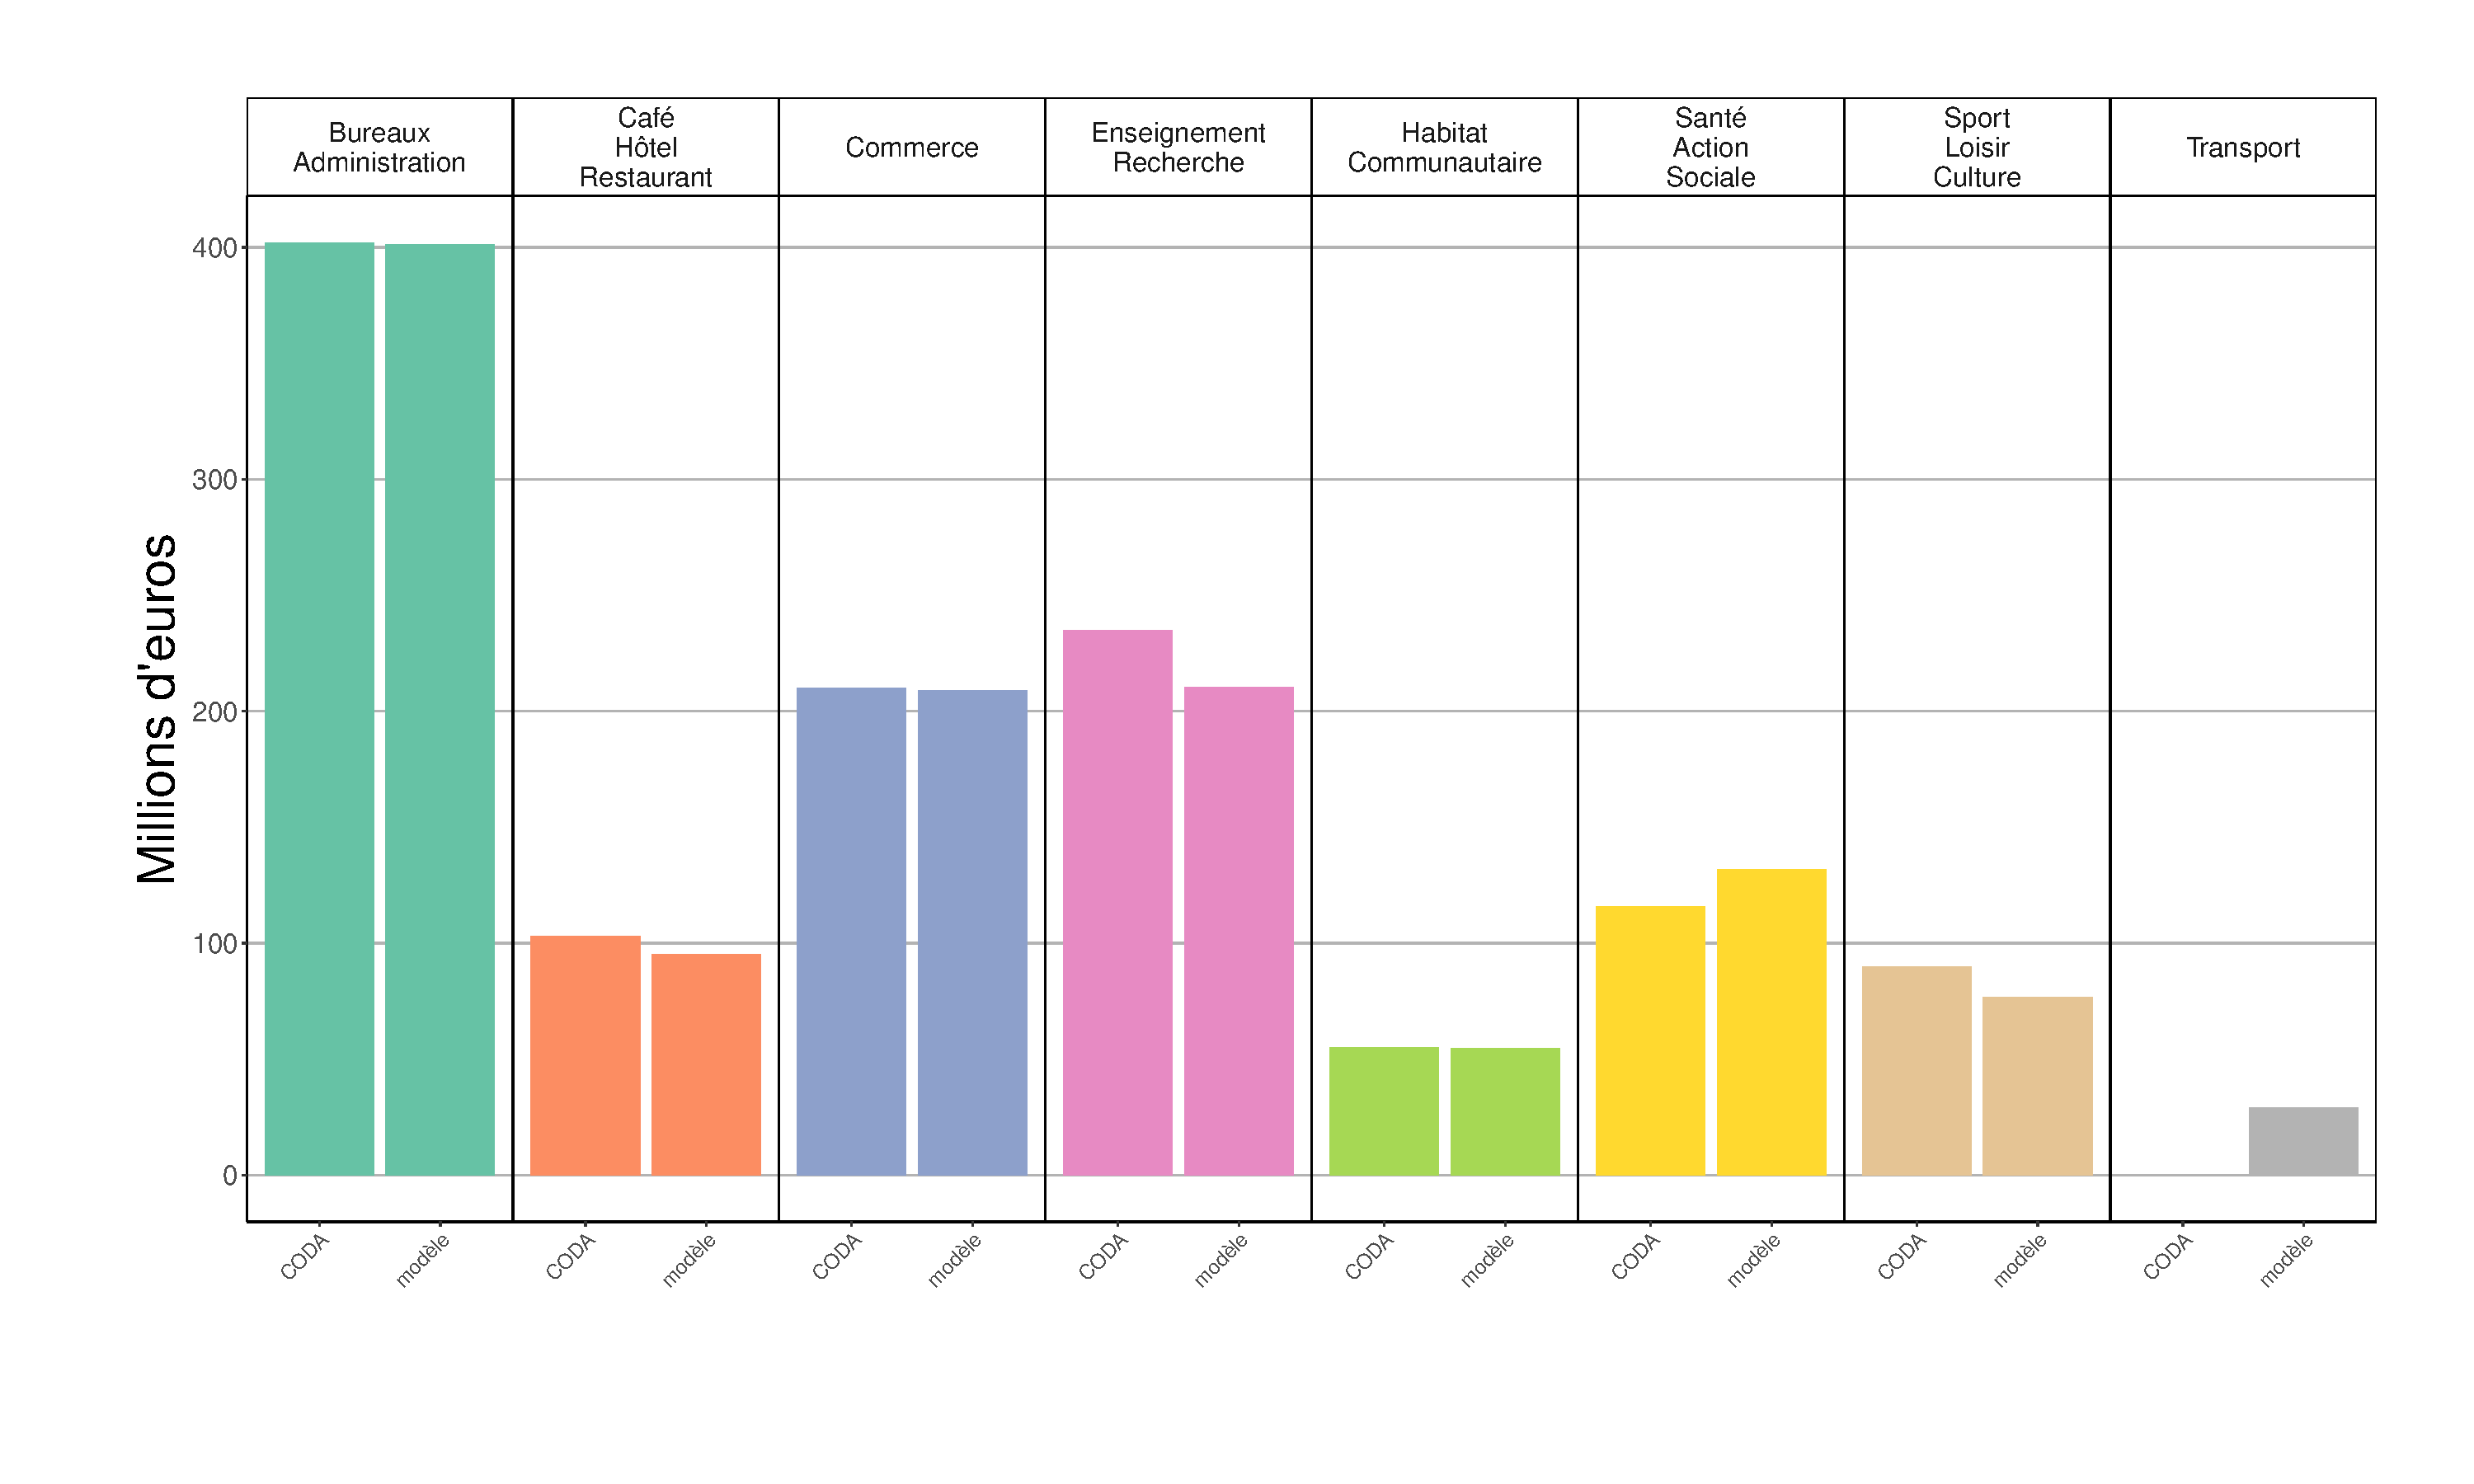
\includegraphics[width = 0.9\textwidth]{Comparaison_Renovbati_CODA}  
\end{figure}

Le modèle simule des investissements d'environ 1.1 milliards d'euros en moyenne entre 2015 et 2020 pour un scénario où les politiques publiques existantes sont maintenus jusque 2020 (cf plus bas pour la définition précise de ce scénario). Ce montant est proche de l'estimation de CODA Strategies de 1.2 milliards d'euros en 2014 à 1.4 milliards d'euros en 2019 (estimation prospective).  

\subsubsection{Changements de systèmes de chauffage dans l'existant}

Selon CODA Strategies, plus d'un tiers du marché de la rénovation tertiaire en 2014 est constitué par des modifications des systèmes de chauffage de ventilation et de climatisation. D'autre part, environ 3\% du parc font l'objet chaque année d'un renouvellement de leur système de chauffage.

Dans le modèle, la part des surfaces qui subissent un renouvellement de système de chauffage est déterminé par la durée de vie des systèmes. En effet, sauf lors d'une rénovation globale de niveau BBC (geste \og~ENSBBC~\fg), les systèmes de chauffage ne sont renouvelés que lors de leur fin de vie. De manière à reproduire le taux de renouvellement observé dans l'étude de CODA Strategies, nous fixons la durée de vie moyenne des systèmes à 33 ans pour obtenir un taux de renouvellement de $\frac{1}{33} \approx 3 \%$. 27 millions de m$^2$ font ainsi l'objet d'une rénovation de leur système de chauffage chaque année. Cette durée de vie est supérieure à celle affichée pour certains systèmes dans les bases de données sur les équipements (ex : Batiprix). Néanmoins, il est courant d'observer des valeurs plus élevées que les durée de vie théoriques des systèmes dans la littérature sur la rénovation énergétique. En rapportant le flux de rénovation aux logements disponibles à la rénovation dans les enquêtes OPEN, Benoît Allibe \citep{Allibe2012} trouve une \og~durée de vie révéleé~\fg des systèmes de 24 ans pour le secteur résidentiel. 

L'étude de CODA Strategies fournit également des estimations des marchés de rénovation par type de système de chauffage. CODA Strategies estime les marchés dans les systèmes de chauffage et la climatisation (hors centrale de traitement d'air) à environ 3 milliards d'euros sur la période de 2014 à 2019. Les sytèmes DRV, multisplit et Rooftop représentent la majeure partie du marché (environ 1 milliard d'euros).  Les chaudières condensation gaz et fioul représentent environ 500 millions d'euros soit 16 \%  du marché. Les systèmes de climatisation à eau glacée représentent près d'un milliard d'euros par an. Le reste du marché est réparti entre les PAC air-eau (225 millions d'euros), les chaudières standard gaz et fioul (200 millions d'euros), les chaudières biomasse (75 millions d'euros) et les convecteurs et rayonnants à effet joule (37 millions d'euros). La comparaison de ces montants avec ceux simulés par le modèle est complexe car les types de systèmes modélisés ne sont pas exactement identiques. D'autre part les investissements liés à la climatisation sont séparés de ceux des systèmes de chauffage dans le modèle. Enfin, le parc tertiaire du modèle et celui de l'étude CODA Strategies diffère légèrement.  

Pour calibrer les parts de marchés des changements de systèmes dans le modèle, on applique des facteurs correctifs aux coûts d'investissements moyens par système présentés plus haut de manière à reproduire les ordres de grandeur des marchés par type de système estimés dans l'étude CODA. Les facteurs correctifs appliqués sont présentés dans le tableau \ref{Coutsystajust}. Cela conduit à augmenter assez fortement la plupart des coûts d'investissement (sauf ceux des PAC qui diminuent). En appliquant ces facteurs correctifs aux coûts moyens des systèmes sur l'ensemble des bâtiments, on modifie les coûts des systèmes tout en gardant des coûts différenciés par type de bâtiment. 

\begin{table}[h!]
\scriptsize
\caption{Ajustement des coûts moyens des systèmes de chauffage dans le modèle}
\label{Coutsystajust}
\begin{center}
\begin{tabular}{l|c|c}
\textbf{Système}	&	\textbf{Coût moyen ajusté} & Facteur correctif \\
									& \textbf{(euros par m²)} &  \\
\\	\hline	\\	
Chaudière gaz	& 40 & 2,6\\	
Chaudière fioul & 30  & 1,5 \\	
Electrique direct	& 20  & 1,9 \\	
PAC	& 60 & 0,9 \\	
Rooftop	& 60  &  1,5 \\		
DRV	& 60 &  2,9\\	
Tube radiant	& 20 & 1,9 \\	
Cassette rayonnante	& 20& 1,9 \\	
Autre système centralisé (Bois et urbain)	& 60 & 1,9 \\	
\hline	
\end{tabular}
\end{center}
\footnotesize{\textbf{ Les coûts affichés ici sont des coûts moyens qui peuvent varier sensiblement d'un bâtiment type à l'autre selon la puissance demandée et la taille du bâtiment. Sources : Bâtiprix, UFE, CGDD}}
\end{table}

La figure \ref{Comparaison_CVCparsyst_CODA} compare les investissements moyens annuels simulés par le modèle sur la période 2015-2020 à ceux estimés par CODA. Le modèle simule des investissements dans les systèmes de chauffage et la climatisation d'environ 3,2 milliards d'euros en moyenne entre 2015 et 2020 ce qui est proche du montant total estimé par CODA Strategies (3 milliards d'euros environ). 

La figure \ref{Comparaison_CVCbranche_CODA} compare les investissements dans le chauffage et la climatisation à ceux de l'étude CODA par branche du secteur tertiaire. 


\begin{figure}[h!]
\centering
\caption{Calibration des montants investis dans les systèmes de chauffage}\label{Comparaison_CVCparsyst_CODA}
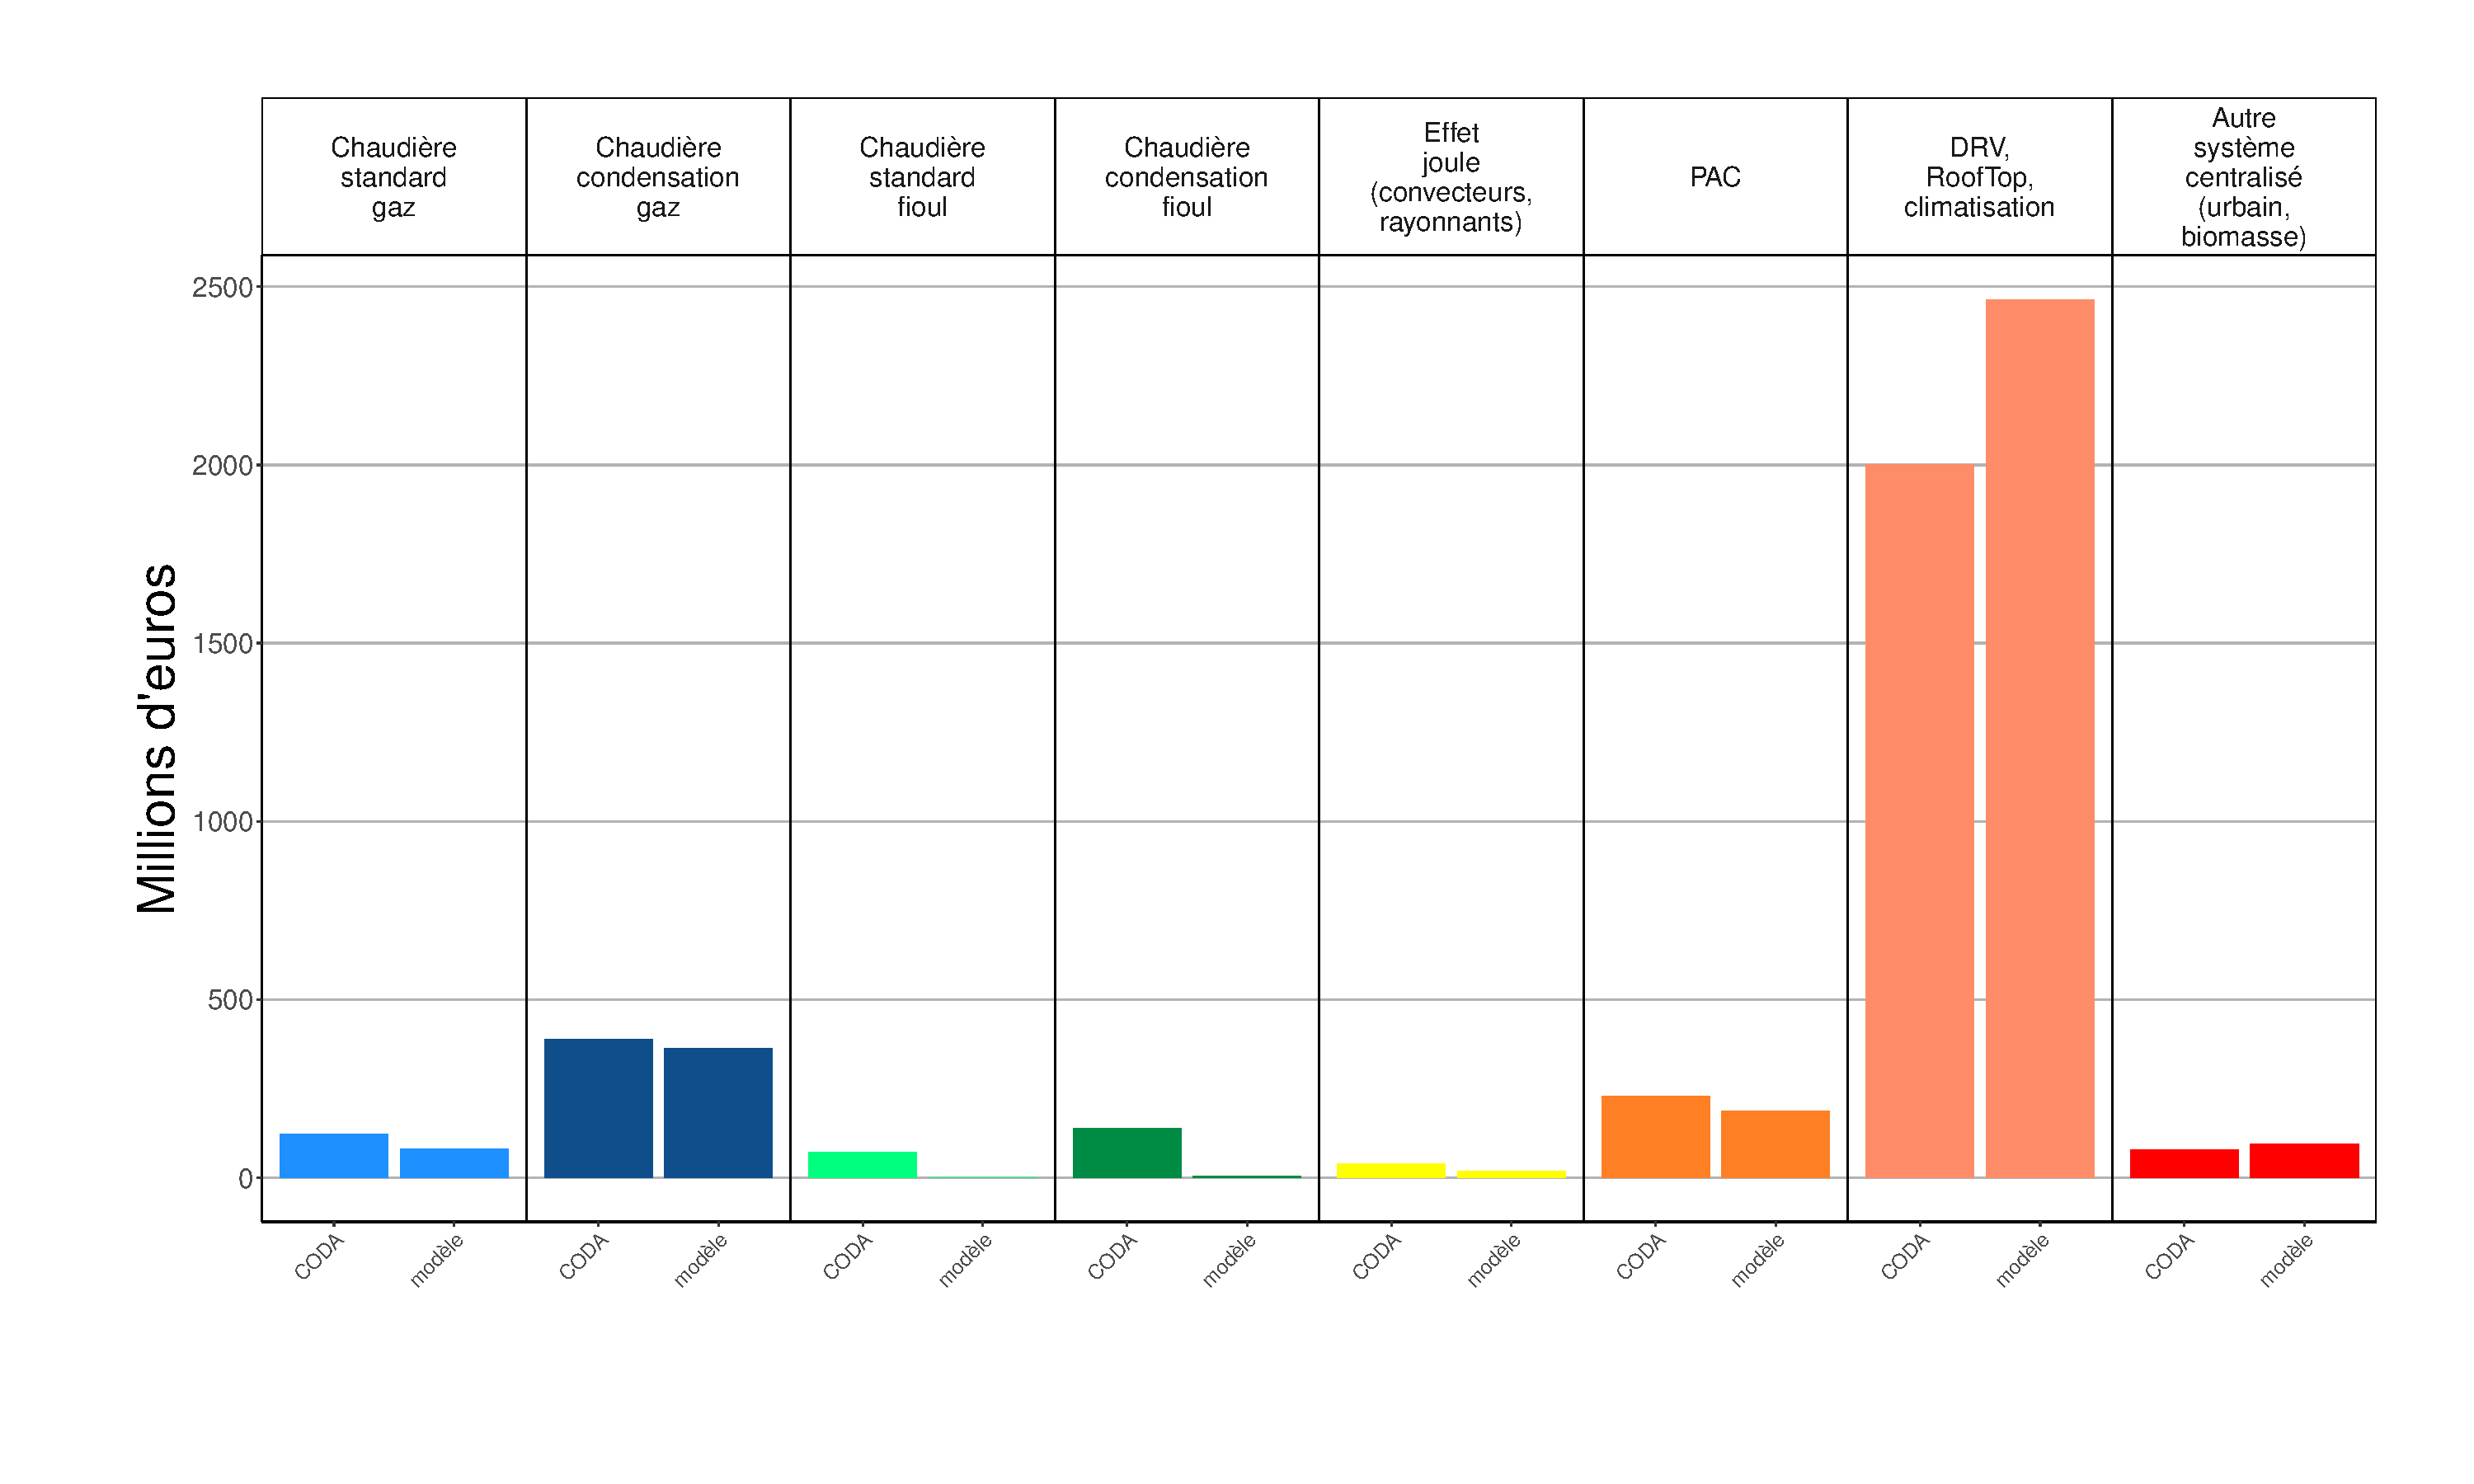
\includegraphics[width = 0.7\textwidth]{Comparaison_CVC_par_systeme_CODA}  
\end{figure}


\begin{figure}[h!]
\centering
\caption{Calibration des montants investis dans les systèmes de chauffage et la climatisation par branche }\label{Comparaison_CVCbranche_CODA}
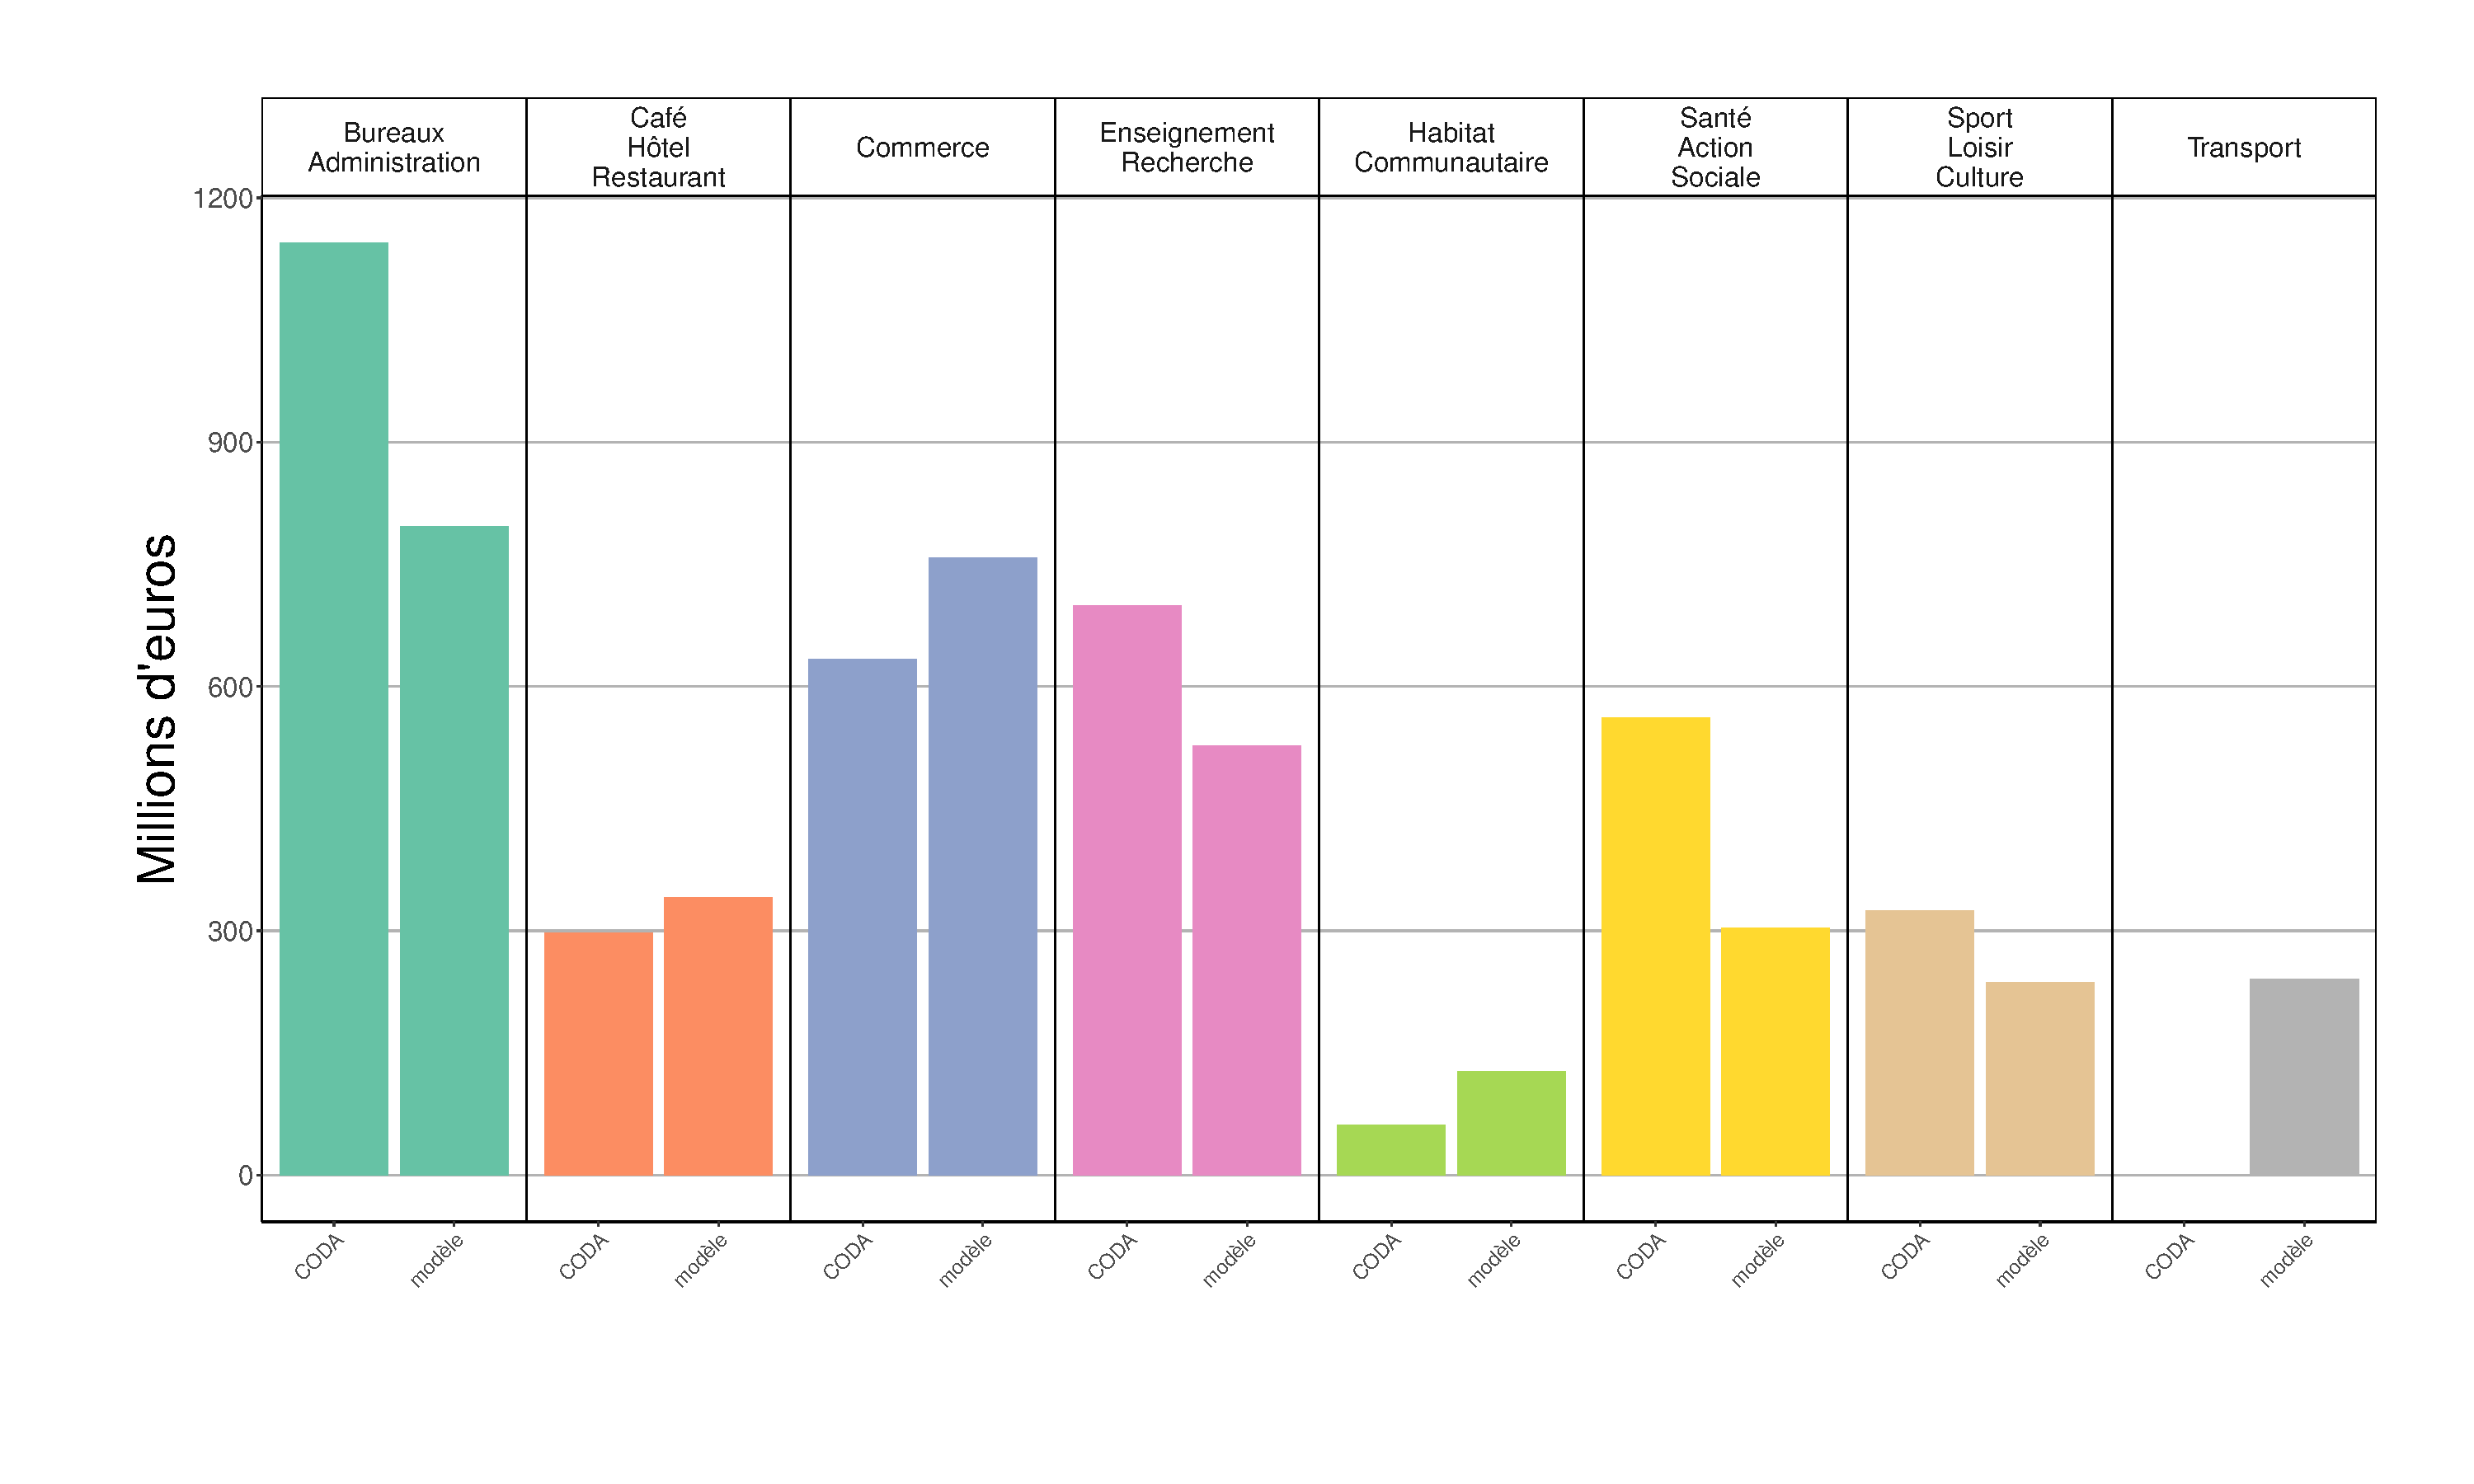
\includegraphics[width = 0.7\textwidth]{Comparaison_CVC_CODA}  
\end{figure}


\subsubsection{Comparaison avec les consommations de chauffage du CEREN}

Les consommations de chauffage dans les sorties du modèle et dans les données du CEREN sont comparées dans la figure ci-dessous. Les évolutions de consommation dépendent de nombreux paramètres dans le modèle, ce qui explique que le calage en 2015 n’est pas parfait. Les consommations totales sont très proches mais la répartition par énergie entre le modèle et les données CEREN diffère légèrement avec notamment une disparition plus rapide du fioul dans les données du CEREN. Les consommations de chauffage évoluent entre 2010 et 2015 selon un rythme similaire dans le modèle (-4,3 \%) et le CEREN (-4,5\%). L’écart initial du niveau de consommations résulte de différences méthodologiques pour la répartition des consommations d’énergie par usage. Un comparaison similaire a été réalisé pour les consommations totales par énergie dont l'évolution est similaire entre le CEREN et les simulations du modèle. 

\begin{figure}[h!]
\centering
\caption{Comparaison des consommations de chauffage par énergie simulées avec les données du CEREN}\label{CompConsoChauffCERREN}
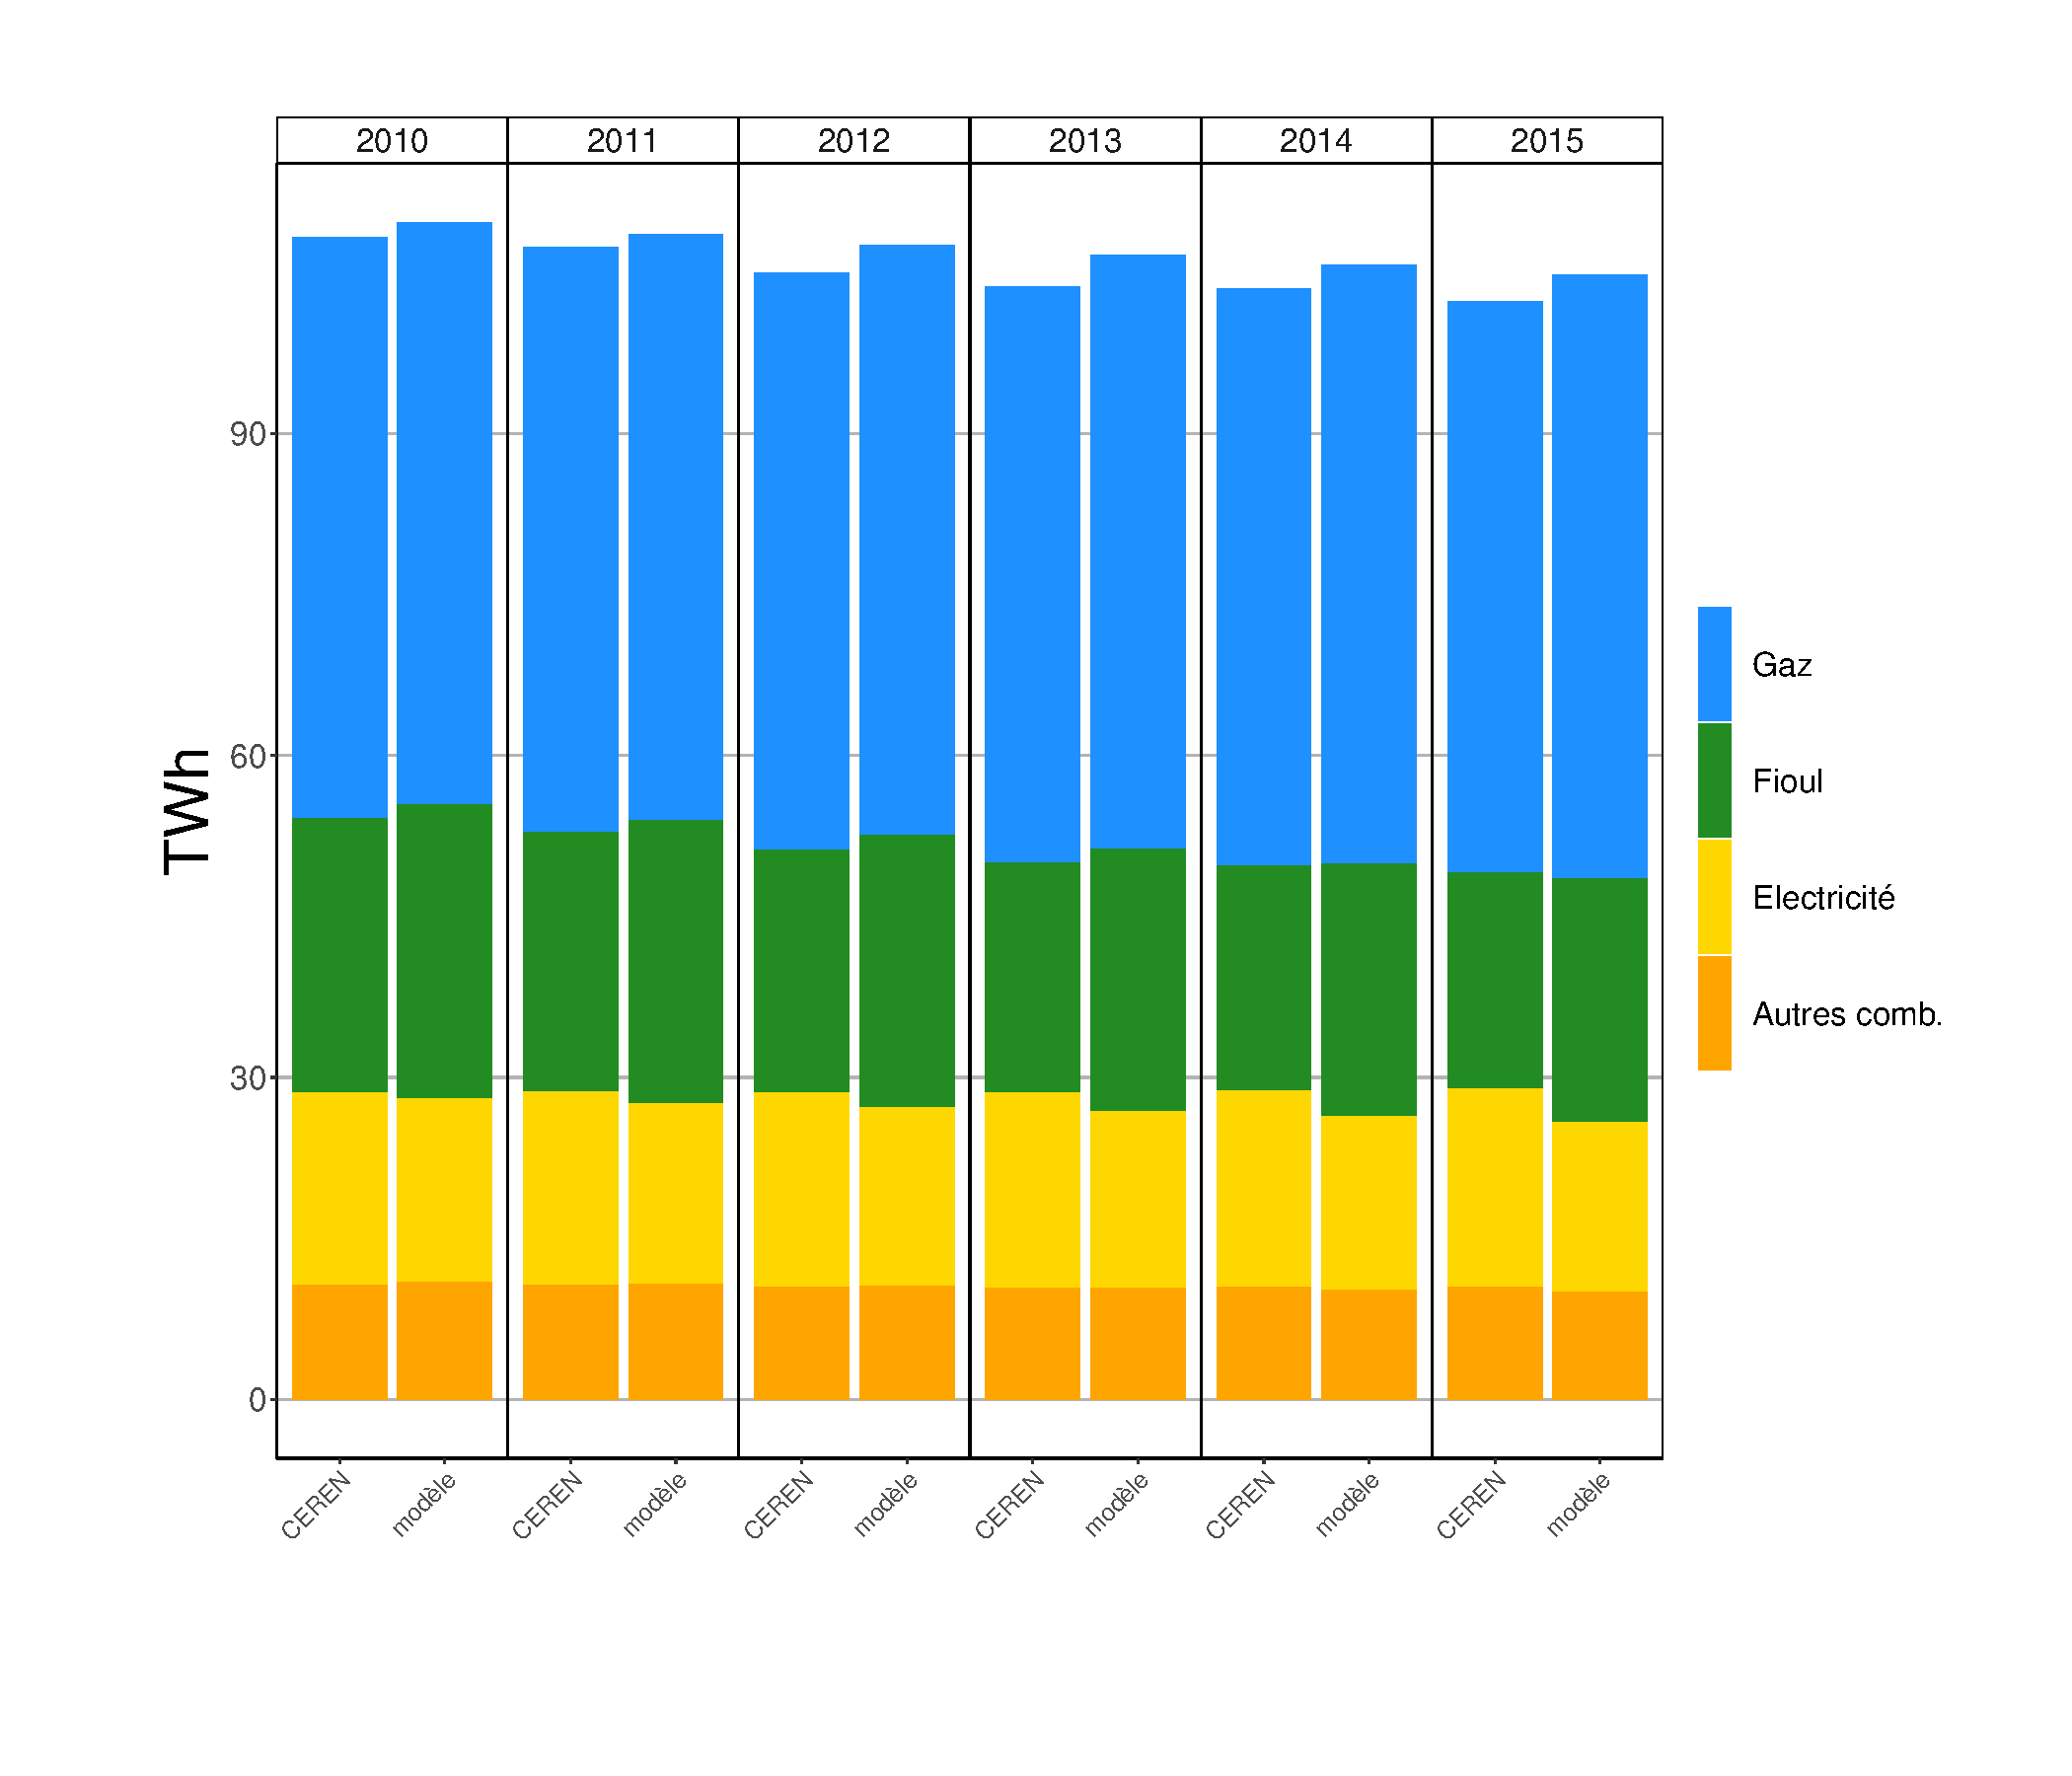
\includegraphics[width = 0.9\textwidth]{CompConsoChauffCERREN}  
\end{figure}


\subsection{Test de sensibilité sur le long terme}

prix constant
prix croissant
lambda

\cleardoublepage

\thispagestyle{partie}
\cadreblanc{Partie 3}{Scénarios}{Résumé Partie}


\newpage
\pagestyle{fancy}

\invisiblesection{Scénarios}\label{sec:marker4}

\markboth{Partie 3 : Scénarios}{}

\textbf{TODO INTRO COURTE}


\subsection{Description des scénarios}

\textbf{TODO A REDIGER}

5 scénarios : 

\begin{itemize}
\item Scénario sans mesures, prix constants en 2018 = scénario P0
\item Scénario sans mesures, prix croissants = scénario de référence
\item Scénario avec mesures existantes, prix croissants + CCE basse = scénario AME
\item Scénario avec mesures additionnelles, décarbonation des énergies en 2050, coûts complets des énergies supportés par l'usager, CCE forte = scénario AMS1
\item Scénario avec mesures additionnelles, décarbonation des énergies en 2050, coûts de décarbonation des énergies subventionnés par l'Etat, CCE forte, composante énergie  = scénario AMS2
\item Scénario avec mesures additionnelles, sans décarbonation des énergies en 2050, CCE forte, composante énergie = scénario AMSDec0
\end{itemize}

mesures AME = mesures votées ou en place au premier juillet 2017
mesures additionnelles très ambitieuses, objectif de neutralité carbone à horizon 2050.

AJOUTER TABLEAU RECAPITULATIF DES SCENARIOS

\subsection{Hypothèses de prix des énergies et de mix énergétique à horizon 2050}


Les évolutions de prix des énergies de 2009 à 2015 sont basées sur l’observation (Base de données pégase).  Pour le scénario  de référence, les évolutions de prix de 2015 à 2050 sont basées sur des taux de croissance annuels moyens provenant d'hypothèses macro-économiques utilisées pour évaluer l'impact de la Stratégie Nationale Bas Carbone sur les consommations des différents secteurs l'économie. Il sont basés soit sur des scénarios de la Commission Européenne (EU reference scenario 2016) soit sur des hypothèses internes (DGEC, ADEME). Pour le gaz, le fioul et la chaleur urbaine , il y a une forte croissance des prix en début de période jusque 2030-2035 puis une croissance moins forte. Pour l'électricité et le bois, les prix croissent à un rythme constant entre 2015 et 2050. 

\begin{table}[h!]
\caption{Taux de croissance annuels moyens des prix des énergies (scénario de référence)}
\begin{center}
\begin{tabular}{|l|c|c|c|c|}
\hline
										& 2015-2030	& 2030-2040	& 2040-2050 &  Sources \\
\hline
Gaz naturel		(à l'importation)									& 	2.6~\%	& 1~\%	& 0.2~\%	 & Commission Européenne \\
Fioul (prix du baril de pétrole)								& 4.5~\%	& 1~\%	& 0.5~\%	 & Commission Européenne\\
Électricité	(production, acheminement...)				& 1.1~\%	& 1.1~\%	& 1.1~\%  & DGEC \\
Chauffage urbain (prix HTVA) 										& 0.8~\%	& 0.2~\%	&  0.2~\%	 & ADEME\\
Bois  (prix HTVA)  															& 1.2~\%	& 1.2~\%	& 1.2~\%	& DGEC \\
\hline
\end{tabular}
\end{center}
\end{table}

Les prix en entrée du modèle sont des prix hors TVA. Il incluent cependant l'ensemble des taxes et des prélèvements fiscaux sur les énergies existant en 2018 notamment la CSPE et la TCFE pour l'électricité, la TICGN pour le gaz et la TICPE pour le fioul. Ces taxes sont supposées stables à leur niveau de 2018 dans l'ensemble des scénarios. Dans les scénarios AME, AMS1, AMS2 et AMSDec0, on ajoute aux prix du scénario du référence des taxes supplémentaires correspondants à des politiques publiques ou des mesures qui s'ajoutent aux évolutions de prix liées au contexte macro-économique. 
 
La composante carbone est incluse à part dans la modélisation. Elle s’applique \textbf{uniquement au gaz et au fioul} dans les scénarios évoqués comme c'est le cas aujourd'hui. La trajectoire utilisée varie selon les scénarios :
\begin{itemize}
	\item scénario P0 et Référence : Composante carbone stable à son niveau de 2018
	\item AME : 56€/tCO2 en 2020 et 100€/tCO2 en 2030, stable de 2030 à 2050.
	\item AMS1, AMS2, AMSDec0 : 225 €/tCO2 en 2030, 400 €/tCO2 en 2040 puis 600 €/tCO2 en 2050.
\end{itemize}

Le niveau de taxation pour chacune des énergies est fonction des taux d’émissions de chaque énergie et donc du mix énergétique utilisé pour les produire.

Dans les scénario P0, Référence, AME, et AMSDec0, le mix énergétique est supposé rester stable dans le temps. Les facteurs d'émissions utilisées pour le calcul de la composante carbone s'appliquant au gaz et au fioul et des émissions liées au gaz et au fioul sont donc stables à leur niveau  de 2015. Pour les autres énergies, la composante carbone est nulle mais les émissions de CO$_2$ dépendent bien des facteurs d'émission de 2015.  

Dans les scénarios AMS1 e AMS2, on considère que l'électricité, le gaz et le chauffage urbain sont progressivement décarbonés à 100\% entre 2015 et 2050. Cela entraîne une baisse progressive du contenu en CO$_2$ de ces énergies mais entraîne un surcoût de production : 
\begin{itemize}
	\item L'incorporation progressive du biogaz (18~\% en 2030, 50~\% en 2040 et 100~\% en 2050) induit un surcoût de production du gaz. On suppose que le coût de production du biogaz progresse 120 et 150~€/Mwh selon le pourcentage de pénétration dans le mix énergétique
	\item L'incorporation progressive d'EnR dans le chauffage urbain (52~\% en 2015, 75~\% en 2030 et 100~\% en 2050) entraîne un surcoût qui augmente avec la part d'EnR (surcoût de 54~€/Mwh lorsque la part d'EnR est de 100 \% par rapport à 2015 où la part d'EnR est de 52~\%)
	\item La production décarbonation progressive de la production d'électricité (50~\% en 2040 et 100~\% en 2050) entraîne un surcoût lié au stockage de l'électricité produite par des EnR qui progresse de 0 à 100~€/Mwh lorsque le mix est décarboné à 100~\% 
\end{itemize}


Les facteurs d'émissions des énergies diminuent proportionnellement à leur décarbonation dans les scénarios AMS1 e AMS2. 

\begin{table}[h!]
\scriptsize
\caption{Facteurs d’émissions utilisés pour le calcul de la composante carbone et des émissions de CO$_2$ liées au chauffage dans le modèle (gCO2/kWh)}
\begin{center}
\begin{tabular}{|l|c|c|c|c|c|}
\hline
																						& 2015-2050							& 2015				& 2030 				& 2050  		 & 2050  \\
																						& P0, REF, AME, AMSDec0 & AMS1, AMS2	& AMS1, AMS2	& AMS1, AMS2 & AMS1, AMS2	\\
\hline
Gaz (CC et émissions) 											& 205										& 205					& 168	 				& 103 			 & 0\\
Fioul	 (CC et émissions)										& 271										& 271					& 271	 				&	271 			 & 271 \\
Électricité	(émissions seulement)						& 180										& 180					& 180  				& 90 				 & 0\\
Chauffage urbain (émissions seulement)	 	  & 146										& 146					&  76	 				& 38 				 & 0\\
Bois (émissions seulement)							  	& 0 										& 0						&  0 					& 0 				 & 0\\
\hline
\end{tabular}
\end{center}
\end{table}


La décarbonation des énergies va entraîner des surcoûts importants qui vont probablement impacter les prix des énergies payés par les usagers ainsi que le budget de l’État si une partie du financement des surcoûts de décarbonation est subventionné.  De manière à étudier l'impact de la décarbonation sur des scénarios contrastés, nous simulons un scénario où les coûts complets de décarbonation se répercutent intégralement dans le prix des énergies payé par les usagers (scénario AMS1) et un scénario dans lequel les coûts de décarbonation sont subventionnnés à 100 \% par l’État (scénario AMS2).  Dans le scénario AMS2 dans lequel les prix des énergies sont bas par rapport à leurs \og~ vrais~\fg coûts, on ajoute une taxe sur toutes les énergies (électricité comprise) entre 2040 et 2050 qui progresse de 0 à 20 €/Mwh qui a pour but d'inciter les usagers à la sobriété énergétique dans un contexte de tension sur les ressources utilisées pour produire les EnR. Dans le scénario AMSDec0, on ajoute également cette composante énergie en fin de période. 

\begin{figure}[h!]
\centering
\caption{Evolution des prix des énergies pour les usagers (HTVA, Composante carbone incluse) dans les différents scénarios}\label{Evol_prix_scen-1}
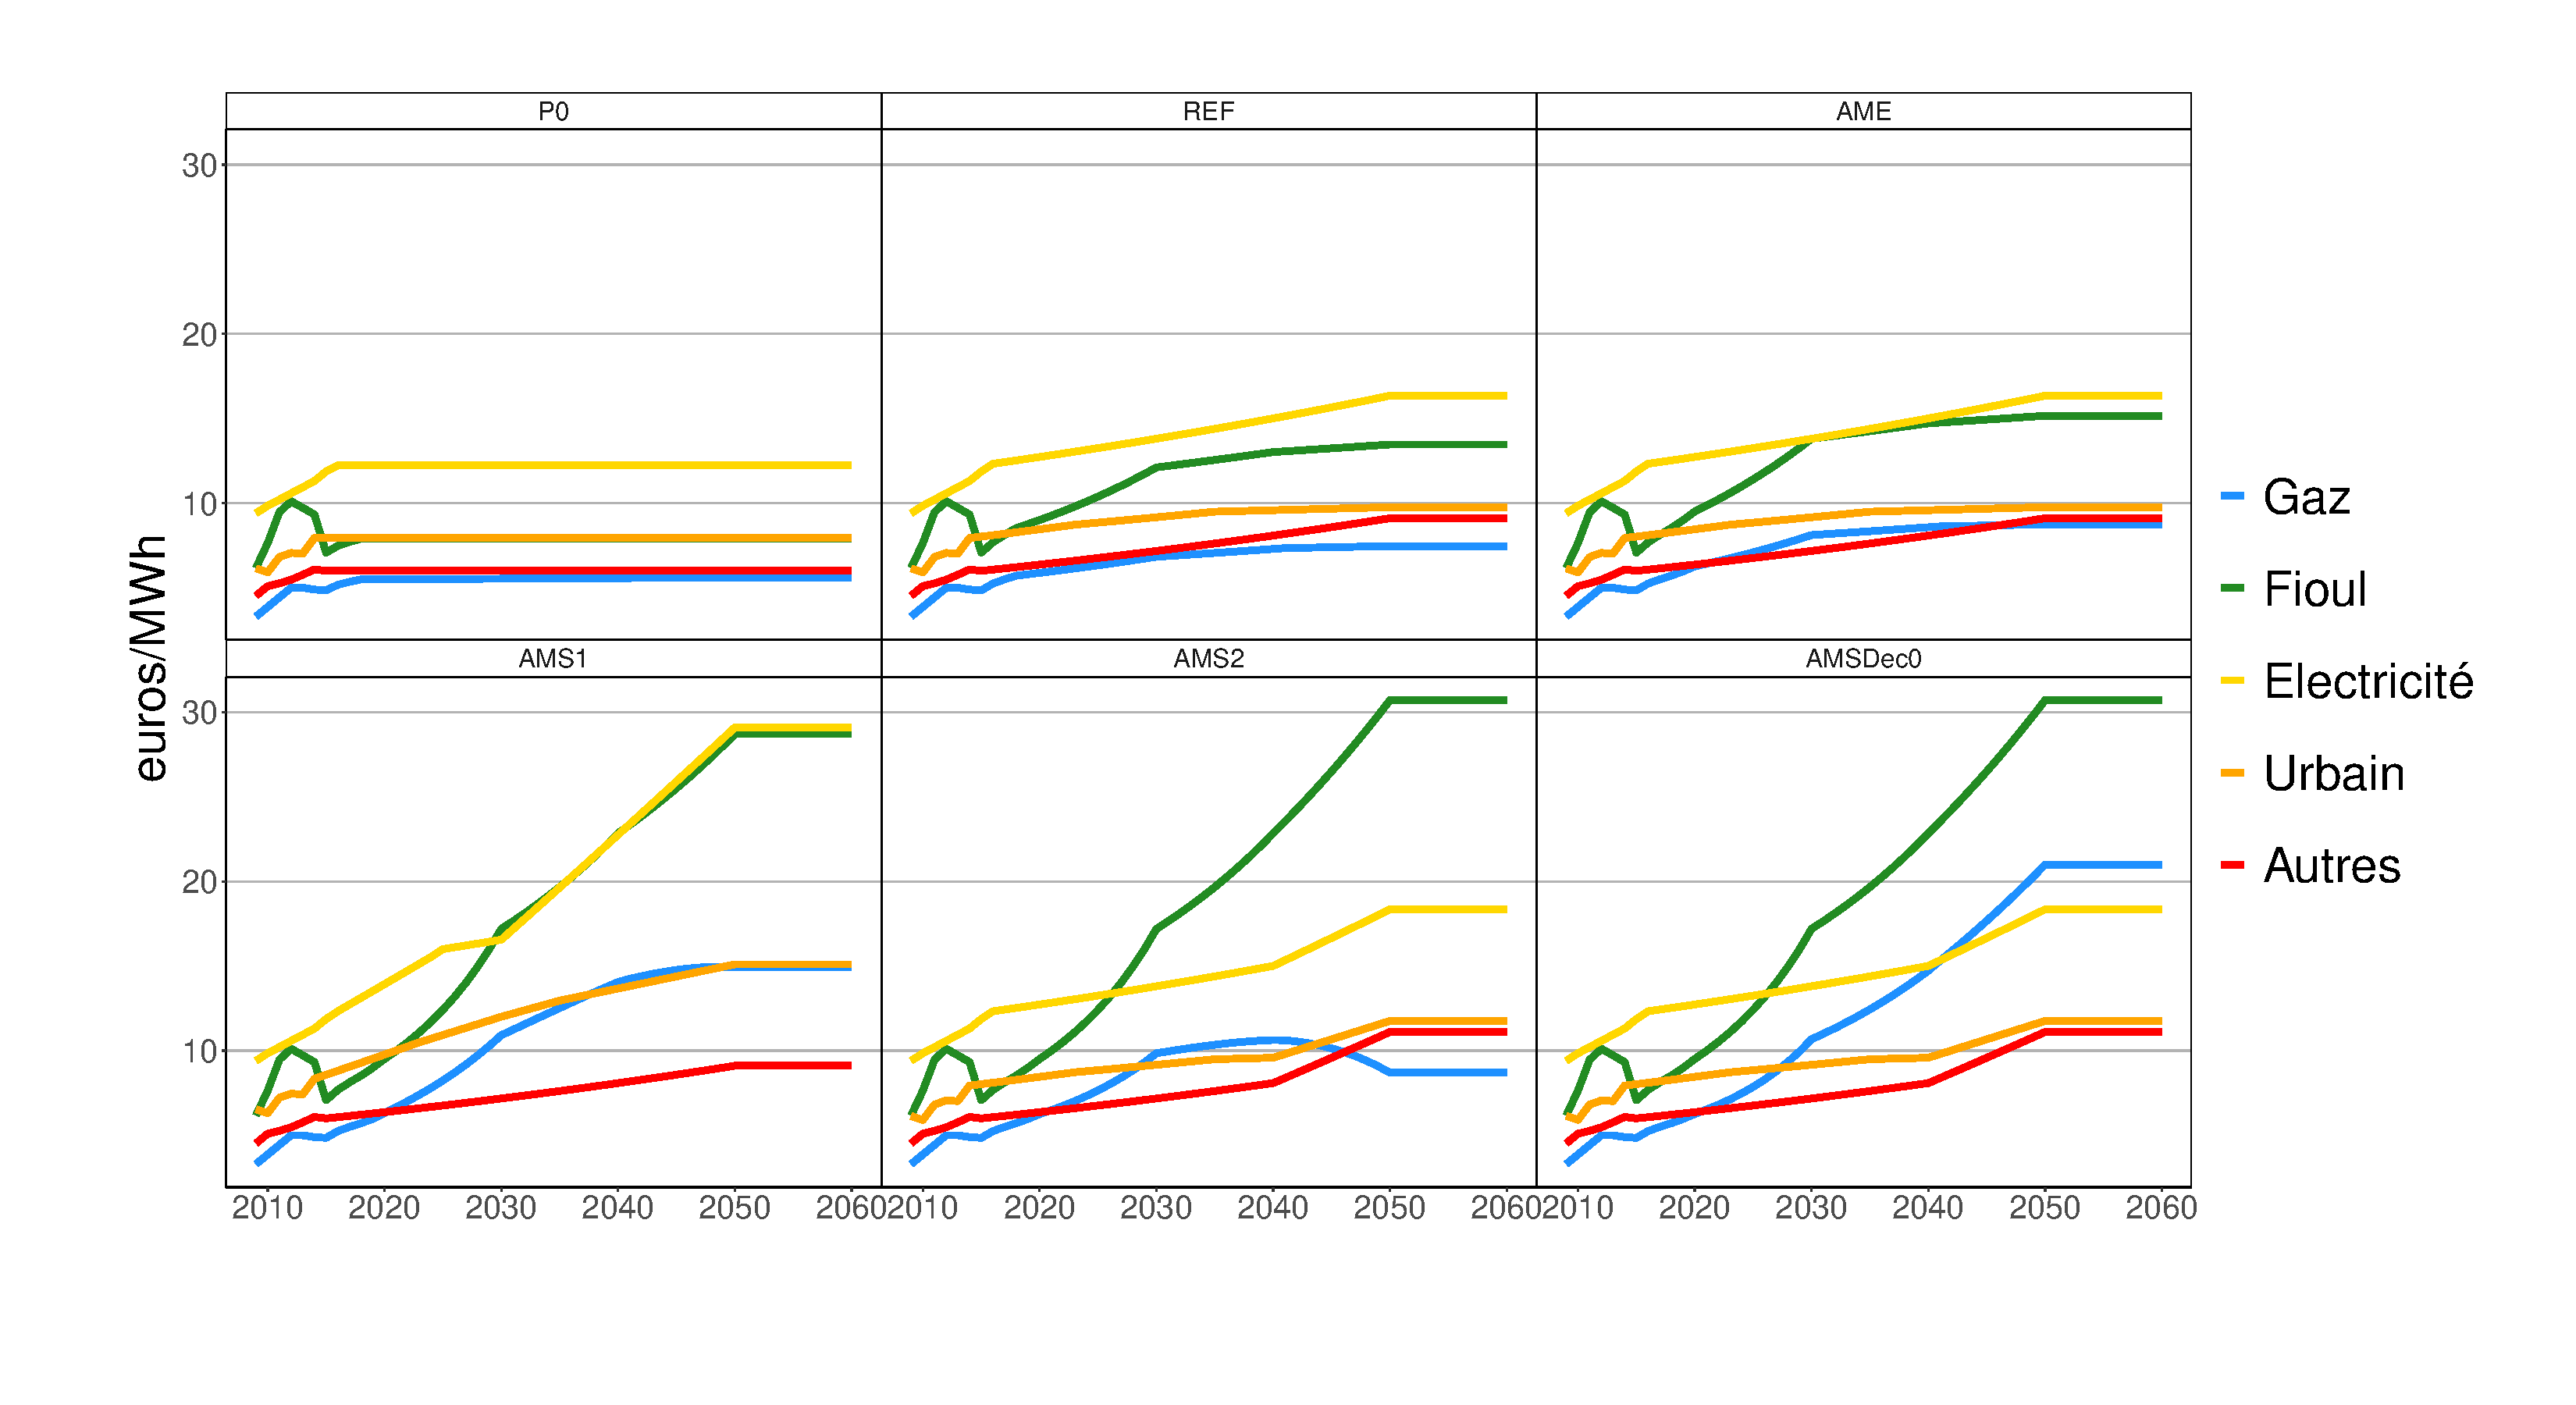
\includegraphics[width = 0.9\textwidth]{Evol_prix_scen-1}  
\end{figure}

\clearpage

\subsection{Mesures et hypothèses sur le parc tertiaire neuf}

\subsubsection{hypothèses de calcul des surfaces entrantes}

L'évolution du parc dans le scénario de référence est issue d'hypothèses macro-économiques sur l’évolution de l’emploi dans le secteur tertiaire et sur des hypothèses sur l’évolution de la surface par employé dans les bureaux et de la surface par habitant pour les autres branches du parc tertiaire. 

Le taux de croissance de l'emploi tertiaire est calculé à partir d'hypothèses sur la valeur ajoutée des services et sur les gains de productivité 

$\textrm{tcam emploi tertiaire} = \textrm{tcam valeur ajoutée des services} – \textrm{gains de productivité}$

Le taux de croissance de valeur ajoutée est donnée par lecadrage macro-économique de la Commission Européenne (EU reference scenario 2016). Faute d’hypothèses sur les gains de productivité des services, on les estime par le calcul suivant :

$\textrm{Gains de productivité} = \textrm{tcam PIB} – \textrm{tcam population}$

\begin{table}[h!]
\caption{Hypothèses sur l'évolution de l'emploi tertiaire}
\begin{center}
\begin{tabular}{|l|c|c|c|c|c|}
\hline
							& 2015	& 2020	& 2025	& 2030	& 2050 \\
\hline
PIB (G€2010)	& 2095	& 2268	& 2419	& 2593	& 3633 \\
Population (millions) & 	64.3	& 65.7	& 66.9	& 68.1	& 71.6 \\
Gains de productivité	& 0.53~\%	& 1.17~\%	& 0.93~\%	& 1.06~\%	& 1.44~\% \\
Valeur ajoutée Services (G€2010) & 	1665	& 1807	& 1925	& 2065	& 2919 \\
Emploi tertiaire (millions)	& 20.2	& 20.7	& 21.0	& 21.4	& 22.7 \\
\hline
\end{tabular}
\end{center}
\end{table}

La répartition de l’emploi par branche en 2015 se base sur des données INSEE. On suppose qu'elle est peu modifiée dans le temps.

\begin{table}[h!]
\caption{Répartition de l'emploi par branche}
\begin{center}
\begin{tabular}{|l|c|c|c|c|c|}
\hline
							& 2015	& 2020	& 2025	& 2030	& 2050 \\
							\hline
Bureaux				&	40\%	& 41~\%	& 41~\% & 42~\%	&42~\% \\
Commerces			& 17~\% &	16~\%	& 15~\%	& 15~\% & 14~\% \\ 
Santé					& 8~\%	& 8~\%	& 8~\%  & 8~\%	&8~\% \\
Autres				& 34~\%	& 35~\% &	35~\% &	35~\% &	36~\% \\
\hline
\end{tabular}
\end{center}
\end{table}

Les surfaces par employés évoluent selon les hypothèses suivantes :  
\begin{itemize}
\item Bureaux : taux de croissance de la surface par employé de 0,2~\%/an, soit un taux historiquement bas correspondant à celui observé sur la période 1995-2005
\item Commerces : surface commerciale par habitant supposée constante (correspond à ce qui est observé depuis 10 ans)
\item Santé : poursuite de l’augmentation de la surface de santé par habitant au même rythme que celui observé depuis 2000
\item Autres : stabilité de la surface par emploi (tendance historique)
\end{itemize}

Les surfaces tertiaires obtenues en multipliant l’emploi par branche aux surfaces par employé sont présentées ci-dessous : 
\begin{table}[h!]
\caption{Surfaces tertiaires par branche en millions de m²}
\begin{center}
\begin{tabular}{|l|c|c|c|c|c|}
\hline
			& 2015	& 	2020	& 	2025	 &	2030		& 2050 \\
\hline
Bureaux		& 221			& 229	& 239 & 	248 & 	270 \\
Commerces	& 211 & 215 & 219 &	223	& 233 \\
Santé	& 114	& 122 & 130 &	138 &	171 \\
Autres	&	420		& 438		& 448		& 457		& 491 \\
\hline
Total	& 966	&	1005 & 1036		& 1066		& 1165 \\
\hline
\end{tabular}
\end{center}
\end{table}

La construction neuve dans le modèle résulte des évolutions de surfaces décrites ci-dessus et des hypothèses sur les taux de destruction par branche.
Les destructions annuelles sont estimées à 2.5 millions de m² par an par GRDF sur la base des données historiques du CEREN relatives aux flux de surfaces tertiaires détruites annuellement. Les taux de destructions par branche dans le modèle sont donc définis de manière à obtenir 2.5 millions de m² détruits en 2015. La répartition par branche se fait en proportion des surfaces existantes en 2009. Les taux annuels de destructions sont maintenus constants de 2015 à 2050. 

Les surfaces neuves (construites après 2009) et existantes obtenues en sortie du modèle sont les suivantes pour les scénarios REF et AME :

\begin{table}[h!]
\caption{Surfaces tertiaires par branche en millions de m² (scénarios REF et AME)}
\begin{center}
\begin{tabular}{|l|c|c|c|c|c|c|}
\hline
Surfaces en millions de m²	& 2010	& 2015	& 2020 & 	2025 & 	2030	& 2050 \\
\hline
Parc < 2009		& 911	& 903	& 890 	& 877		& 865			& 820 \\
Parc >= 2010	& 10	& 63	& 112		& 152		& 194			& 345 \\
TOTAL					& 921	& 966	& 1002	& 1029 	& 1059	 	& 1165 \\
\hline
\end{tabular}
\end{center}
\end{table}

Pour le scénario AMS, on fait l’hypothèse d’une baisse de la construction neuve après 2020 (développement du coworking, télétravail...) 

\begin{table}[h!]
\caption{Surfaces tertiaires par branche en millions de m² (scénarios AMS)}
\begin{center}
\begin{tabular}{|l|c|c|c|c|c|c|}
\hline
Surfaces en millions de m²	& 2010	& 2015	& 2020 & 	2025 & 	2030	& 2050 \\
\hline
Parc < 2009		& 911	& 903	& 890 	& 877		& 865			& 818 \\
Parc >= 2010	& 10	& 63	& 112		& 148		& 186			& 319 \\
TOTAL					& 921	& 966	& 1002	& 1026 	& 1051	 	& 1137 \\
\hline
\end{tabular}
\end{center}
\end{table}

\subsubsection{Réglementation thermique dans le neuf}

Les réglementations thermiques constituent la principale mesure impactant le parc neuf. Les tableaux ci-dessous montrent la part des constructions de bâtiments tertiaires neufs respectant la RT2012 selon les périodes de construction pour le scénario AME. Les besoins unitaires pour les usages réglementés (en kWhEF/m²) par branche sont représentés sur le graphique suivant. Les besoins unitaires des bâtiments entrants sont les mêmes quelle que soit l’énergie de chauffage. Pour les systèmes électriques joules, on ajoute donc au coût d’investissement un surcoût de 20 euros par m² (hypothèse CGDD à partir des données de l’enquête ICC-PRLN) pour tenir compte du fait que la RT 2012 entraîne un surcoût d’isolation pour les bâtiments entrants avec un système électrique joule, car les critères de performance énergétique sont en énergie primaire.

Pour les scénarios REF et AME, les besoins unitaires des bâtiments entrants sont conformes à la RT 2012 de 2012 à 2050.

\textbf{TODO GRAPH BESOINS UNITAIRE PAR BRANCHE}

Pour les scénarios AMS, afin de prendre en compte de futures réglementations thermiques et l’amélioration de l’efficacité énergétique des équipements, l’hypothèse retenue est de faire baisser les besoins unitaires des bâtiments entrants progressivement entre 2020 et 2050 :

\begin{itemize}
	\item Besoins de chauffage : par rapport à 2015, -5~\% en 2030, -15~\% en 2040 et  -30~\% en 2050 
	\item Besoins des autres usages : par rapport à 2015,  -5~\% en 2030, -10~\% en 2040, -20~\% en 2050
\end{itemize}

NB : les surcoûts de construction liés à ces mesures ne sont pas comptabilisés dans le modèle.

\subsubsection{Bâtiments exemplaires de l’État (arrêté du 10 avril 2017), scénarios AME et AMS }

La LTECV prévoit que toutes les nouvelles constructions publiques (bâtiments de l’Etat et des collectivités) seront exemplaires au plan énergétique et environnemental à chaque fois que possible. Il est supposé que 50~\% des surfaces neuves construites par l’Etat et les collectivités sont exemplaires à partir de 2016, les 50~\% restants étant au niveau RT 2012. 

Les besoins unitaires des bâtiments entrants dans le modèle sont modifiables par période uniquement (2010-2015, 2016-2020, 2021-2030, 2031-2040, 2041-2050). Pour faciliter la modélisation, nous prenons donc en compte la mesure dès 2016 même si l’arrêté date de 2017. 

L’étude d’impact de la mesure indique une répartition selon les niveaux de performance E+C- dans les grands bureaux de 10~\% pour le niveau 1, 40~\%pour le niveau 2, 40~\% pour le niveau 3 et 10~\% pour le niveau 4. A ces niveaux de performance correspondent une baisse de la consommation des usages réglementés de -15~\%, -30~\% et de -40~\% pour les niveaux 3 et 4. On obtient donc une répartition du parc entrant et une baisse des besoins unitaires selon le tableau suivant : 

\begin{table}[h!]
\begin{center}
\begin{tabular}{|l|c|c|}
\hline
				&	Part des bâtiments neufs selon  & Baisse du besoin unitaire pour les \\
				& le niveau de performance				& usages RT par rapport à la RT 2012 \\
				\hline
				
E+C- 1	& 5~\% 	& -15~\% \\ 
E+C- 2	& 20~\% 	& -30~\% \\
E+C- 3	& 20~\% 	& -40~\% \\
E+C- 4	& 5~\% 	& -40~\% \\
RT2012	& 50~\% 	& 0~\% \\
\hline
\end{tabular}
\end{center}
\end{table}

On corrige les besoins unitaires des usages RT pour l’ensemble des bâtiments neufs entrants de l’État après 2016 par un facteur égal à  $0.05*(1-0.15) + 0.2*(1-0.3) + 0.2*(1-0.4) +0.05*(1-0.4) + 0.5*1 = 0.8325$

\subsection{Mesures sur le parc existant}

\subsubsection{Directive européenne « Patrimoine de l’État : efficacité énergétique » }

La directive « Patrimoine de l’État : efficacité énergétique » vise à rénover les bâtiments de l’Etat qui ne satisfont pas à la réglementation thermique, ce qui a été évalué quantitativement à rénover 3~\% du parc de l’Etat par année, sur la période 2014-2020. Dans les faits, la France a choisi d’avoir une approche alternative, car les lois Grenelle I et II votées en 2009 et 2010 fixent déjà un objectif de réduction de 40~\% des consommations énergétiques des bâtiments de l’État, entre 2012 et 2020. Pour le scénario AME, il a été décidé de prolonger le rythme de rénovation de 3~\% par an après 2020.

Dans le cadre de la modélisation du scénario AME, une obligation de rénovation de 3~\% par an du parc appartenant à l’État sur la période 2014-2050 a été introduite dans le modèle afin de faciliter la modélisation. Pour les scénarios AMS, on porte cette obligation de rénovation à 5~\% du parc de l’État par an à partir de 2018 (1 quart du parc de l'État rénové durant le quinquennat actuel).

En 2010, le parc de l’État représente 90 millions de m² dans le modèle. Les surfaces rénovées annuellement en millions de m² sont de l'ordre de 2.8 et 3.8 millions de m² par an  pour le scénario AME et les scénarios AMS respectivement. La part du parc non rénové de l’État diminuant dans le temps, les surfaces rénovées du fait de la réglementation diminuent également à mesure que le gisement s’épuise. L’obligation de rénovation n’est pas la seule mesure qui s’applique au parc de l’État, les surfaces rénovées peuvent donc varier dans le temps du fait des autres mesures impactant le parc (CEE, travaux embarqués, prix des énergies…).

%\textbf{AJOUTER Tableau surfaces rénovées ici ???}

\subsubsection{Certificats d’économie d’énergie : }

Les CEE pour la première et la seconde période sont considérés comme intégrés aux rénovations diffuses avant 2015 c'est à dire qu'elles ne sont pas modélisées .

La 3ème et la 4ème période des CEE sont intégrées dans le modèle à travers une subvention sur les économies d'énergie provenant des gestes sur le bâti et des changements de systèmes de chauffage. Chaque geste et système de chauffage est associé à une quantité de CEE en kWh cumac calculée à partir des fiches CEE. La subvention est proportionnelle aux kWh cumac générés par chaque geste ou changement de système.

Pour le scénario AME, le niveau de la subvention par CEE est fixé à 5 euros/ MWh cumac pour la 3ème période et à 6 euros/MWh cumac pour la 4ème période. Le signal prix correspondant aux CEE s’arrête en 2020. Pour le scénario AMS, on maintient la subvention après 2020 et son niveau croît de 1,2~\% par an jusque 2030 puis de 7~\% par an jusque 2050. Le niveau de la subvention par CEE atteint 26 euros par MWhcumac en 2050. Cela correspond à une subvention d’environ 45~\% du montant des investissements réalisés en 2050. Cela peut paraître élevée mais assez comparable au niveau de subvention correspondant à l'ensemble des aides existant actuellement pour la rénovation énérgétique dans le secteur résidentiel. 

	

\begin{table}[h!] \caption{Valeurs moyennes des CEE en  kWh cumac par m² accordés par geste et système}
\begin{center}
\begin{tabular}[c]{|l|c|}
\hline
Geste sur le bâti 	& CEE accordés	 \\
\hline
ENS\_BBC						& 2500 \\
ENS\_MOD						& 1800 \\
FENMUR\_BBC					& 1800 \\
FENMUR\_MOD					& 1100 \\
FEN\_BBC						& 1000 \\
FEN\_MOD						& 1000 \\
GTB									& 0 \\
\hline
\end{tabular}
\\
\begin{tabular}[c]{|l|c|c|}
\hline
													& \multicolumn{2}{c}{CEE accordés} 	\\
													\hline
Système de chauffage			& Non performant	& performant \\
\hline
Chaudière fioul						& 0	& 800 \\
Chaudière gaz							& 300	& 800 \\
Tube radiant							& 500	& 500 \\
PAC												& 700	& 700 \\
DRV												& 800	& 800 \\
Rooftop										& 700	& 700  \\
Électrique direct					& 0	& 0 \\
Cassette rayonnante				& 0	& 0 \\
Autre système centralisé	& 400	& 400  \\
\hline
\end{tabular}
\end{center}

\footnotesize{NB : les valeurs des CEE accordés sont données par les fiches CEE et varient selon le type de bâtiment concerné. Ce sont ici des valeurs moyennes sur l’ensemble du parc. }
\end{table}

\subsubsection{Obligation de rénovations énergétiques lors de travaux importants (« Travaux embarqués »)}

Cette mesure vise à obliger les propriétaires de bâtiments à intégrer des travaux d'isolation thermique par l'extérieur lorsqu'ils réalisent des travaux de rénovation importants sur leurs bâtiments comme un ravalement. 

L’étude d’impact de la mesure sur le secteur tertiaire estime que chaque année, environ 4,8 millions de m² feront l’objet d’un ravalement en application de décret et 8,5 millions de m² feront l’objet d’une réfection de toiture ce qui correspond à environ 1,5~\%  du parc tertiaire. Les économies d’énergie annuelles correspondantes sont estimées à 375 GWh. 

Les gestes ravalements et réfection de toiture seuls ne sont modélisés dans le modèle que dans des bouquets avec d’autres gestes. Pour modéliser la mesure, il a été choisi d’augmenter le taux de rénovation de l’ensemble du parc de manière à reproduire les économies d’énergie décrites ci-dessus (375 GWh annuelles). Cela nécessite d’augmenter le taux de rénovation tendanciel de l’ensemble du parc de 1~\% à partir de 2017. Ce taux additionnel est maintenu jusque 2050. Cette mesure est incluse dans le scénario AME et dans les scénarios AMS. 

\subsubsection{Réglementation thermique pour les travaux de rénovation dans les bâtiments existants (RT existant 2018) et Directive Eco-conception :}

L’arrêté concernant la nouvelle Réglementation thermique pour les rénovations dans les bâtiments existants a été publié en mars 2017. Elle impose un niveau minimal de performance des gestes d'isolation du bâti supérieur à la précédente.

Le modèle permet d’imposer un niveau minimal de performance lors d’une rénovation : niveau modéré qui correspond à la RT élément par élément précédente ou niveau BBC rénovation. 

Le niveau BBC étant plus performant que le niveau de la nouvelle RT par élément, la mesure a été modélisée en augmentant les gains des gestes modérés de 6~\%  à partir de 2018 (hypothèse prise sur l’analyse de surcoûts sur des bâtiments types par la DHUP). Les coûts d’investissements des gestes modérés ont été augmentés de 9~\%  (surcoûts moyens sur bâtiments types de la DHUP). 

En ce qui concerne les systèmes de chauffage, il n’a pas été possible de formaliser des hypothèses système par système pour prendre en compte l'impact de la Directive européenne Ecodesign qui impose des niveaux minimums de performance des systèmes. On applique ainsi une hausse de 10~\%  des rendements des systèmes non performants (niveau de performance minimum des systèmes dans le modèle) et un surcoût de 15~\%. Cette mesure est incluse dans le scénario AME et dans les scénarios AMS. 

\subsubsection{Individualisation des frais de chauffage}

Le décret d'application de la LTECV sur l’individualisation  des  frais  de  chauffage  vise faire installer des appareils de mesure permettant de déterminer la quantité de chaleur consommée de chaque occupant d'un immeuble chauffé de manière collective.  Sur la base de l’étude d’impact de la mesure, la part du parc tertiaire chauffée par un système collectif a été estimée à 30~\%. 15~\% de ces surfaces font l’objet d’une impossibilité technique. La part du parc total équipé est donc $0,3*(1-0,15) = 25,5$~\%. Le gain attendu sur les besoins de chauffage du parc cible est estimé à 7,5~\%. On suppose que le parc cible est équipé en 3 ans. Cela conduit à diminuer le besoin unitaire de chauffage du parc total dans le modèle comme indiqué dans le tableau suivant  :
	
\begin{table}[h!] \caption{Baisse du besoin unitaire de chauffage du fait de l’individualisation  des  frais  de  chauffage}
\begin{tabular}[c]{|l|c|c|c|c|}
\hline
																									& 2016 & 	2017 	&	2018 	&	2019	\\
\hline																									
part du parc éligible équipé											& 0~\% & 33~\%	& 67~\% &	100~\% \\
part du parc tertiaire total équipé 							&	0~\% & 8,5~\%	&17,0~\%&	25,5~\% \\
Évolution du besoin de chauffage du parc total (indice) 		& 1	& 0,994	&	0,987	& 0,981 \\
\hline
\end{tabular}
\end{table}

Les gains sont maintenus jusqu’en 2050. Cette mesure n’entraîne pas de surcoûts dans le modèle. Cette mesure est incluse dans le scénario AME et dans les scénarios AMS. 

\subsubsection{Décret d'obligation de rénovation du parc tertiaire (scénario AMS uniquement) :}

Dans les scénarios AMS, on modélise l'impact d'un futur d'obligation de rénovation du parc tertiaire. Dans le modèle, le décret est modélisé au niveau de la branche et de l’occupant à l'aide de 6 paramètres :

\begin{itemize}
	\item Part des surfaces concernées par le décret
	\item Temps de retour sur investissement maximal (en années)
	\item Investissement maximal (en euros par m²)
	\item Gain minimal attendu sur les consommations d’énergie primaire des usages RT (en \%)
	\item Année d’entrée en vigueur du décret
	\item Année de fin d’application
\end{itemize}

Pour les scénarios AMS, il a été décidé d’appliquer le décret à tous les bâtiments de plus de 500 m² avec des exigences de baisse de consommations plus faibles pour les petits bâtiments que pour les grands. Le gain minimal sur les consommations d’énergie primaire des usages RT est fixé à :

\begin{itemize}
	\item -60~\%	sur les bâtiments de plus de 2000 m²
	\item -50~\%sur les bâtiments de 1000 à 2000 m²
	\item -40~\% sur les bâtiments de 500 à 1000 m²
\end{itemize}

Dans le modèle, au sein de chaque branche, différents types de bâtiments existent. Chaque type de bâtiment est défini par une surface moyenne variable et par la surface totale qu’il occupe dans le parc. Pour définir la surface concernée par le décret et le gain minimal attendu sur les consommations dans la branche, on calcule dans chaque branche la part de la surface occupée par des bâtiments de surface moyenne de plus de 2000 m², de 1000 à 2000 m² et de 500 à 1000 m². La surface concernée par le décret est la surface de tous les bâtiments de plus de 500 m². Le gain minimal sur la branche est calculé en pondérant les surfaces de chaque taille de bâtiments par les gains minimaux définis ci-dessus (-60~\%,-50~\% et -40~\%)
Par exemple, pour la branche « Café Hôtel Restaurant », le gain minimal sur les consommations attendu est de $(0,13*0,60 + (0,24-0,13)*0,5 +(0,38-0,24)*0,4)/0,38 = 48.9~\% $

Le tableau ci-dessous donne les parts des surfaces concernées par le décret et les baisses de consommation minimales par branche du parc.
Le décret couvre ainsi environ 61,5~\% du parc et impose un gain minimal moyen de 53,6~\% sur les consommations des usages RT (Chauffage, ECS, climatisation, ventilation, éclairage)

\begin{table}[h!] \caption{Décret de rénovation du parc tertiaire}
\scriptsize
\begin{tabular}[c]{|l|c|c|c|c|c|}
\hline
												& Part des bâtiments 	& Part des bâtiments 	&	 Part des bâtiments 	&	Part de la surface  &	Baisse minimale  \\
												& > 2000 m² 					& > 1000 m²						& > 500 m² 							& concernée par le décret &   de consommation \\
\hline
Bureaux Administration	&	42~\% &	42~\% &	42~\% &	42~\% &	60,00~\% \\
Café Hôtel Restaurant		& 13~\% &	24~\% &	38~\% &	38~\% &	49,9~\% \\
Commerce								&	16~\% &	45~\% &	48~\% &	48~\% &	52,6~\% \\
Enseignement Recherche	&	65~\% &	76~\% &	96~\% &	96~\% &	54,6~\% \\
Habitat Communautaire		&	0~\% &	42~\% &	89~\% &	89~\% &	44,7~\% \\
Santé Action Sociale		& 55~\% &	55~\% &	83~\% &	83~\% &	53,3~\% \\
Sport Loisir Culture		&	21~\% &	35~\% &	41~\% &	41~\% &	53,7~\% \\
Transport								& 17~\% &	37~\% &	37~\% &	37~\% &	54,6~\% \\
\hline
Total										&	35,01 ~\% &	48,86~\% &	61,5~\% &	61,5~\% &	53,6~\% \\
\hline
\end{tabular}
\end{table}

L’obligation de rénovation s’applique uniformément à tous les bâtiments d’une même branche. La baisse de consommation minimale est divisée par le nombre d’année d’application du décret. Pour le scénario AMS, le décret est appliqué de 2015 à 2050 ce qui impose une baisse moyenne des consommations de 1,7 ~\% par an. Pour chaque type de bâtiment, le modèle évalue chaque année parmi les gestes de rénovation possibles ceux qui satisfont les critères du décret : gain minimal, temps de retour sur investissement et coût maximal au m². Si aucun geste ne satisfait ces critères, le décret n’a pas d’impact sur ce segment du parc. Si plusieurs gestes satisfont les critères, on retient le plus rentable (coût global le plus faible). Le temps de retour sur investissement maximal est fixé à 30 ans et le coût maximal à 2000 euros par m².

\subsubsection{Prêts bonifiés à destination des collectivités (scénario AMS uniquement) :}

Une mobilisation de 3 milliards en faveur des travaux de rénovation des collectivités locales d’euros a été annoncée dans le Plan Rénovation en avril 2018. Pour les scénarios AMS, on modélise ainsi la possibilité pour les collectivités de financer leurs travaux de rénovation par un prêt bonifié à 1~\% si un geste de rénovation de niveau BBC est réalisé. Ce prêt est limité à 1 000 000 d’euros sur 10 ans. On maintien ces prêts bonifiés jusque 2050. Sur la période du quinquennat, le modèle simule 3.7 milliards d’euros de prêts bonifiés (montant des investissements financés par les prêts bonifiés). 

\subsection{Hypothèses sur les usages hors chauffage}

\subsubsection{ECS}

Les rendements des systèmes d’ECS évoluent à la hausse de manière tendancielle lors du renouvellement en fin de vie des systèmes (pénétration des systèmes performants et des ballons thermodynamiques). On suppose une pénétration de 5 à 10~\% selon la branche du parc des panneaux solaires thermiques lors du renouvellement des systèmes en fin de vie et entrant dans le parc avant 2030, puis de 10 à 20~\% après 2030. 

Dans le scénario AMS, on fait l’hypothèse d’une pénétration plus rapide des systèmes performants qu’en AME. 100~\% des systèmes installés en 2030 sont performants (50~\% en AME). D’autre part on introduit une baisse progressive de 20~\% du besoin unitaire en ECS entre 2015 et 2050 pour tenir compte de la pénétration d’équipements (hors système de production) plus performants (ex : mitigeurs). Enfin, on fait l’hypothèse d’une hausse du rendement des ballons thermodynamique de 1,8 à 2,5. La baisse du besoin en ECS et la hausse du rendement des ballons thermodynamiques n’entraînent pas de surcoûts dans le modèle.

\subsubsection{Climatisation}

Les taux de climatisation dans le parc existant augmentent annuellement de 1~\% jusqu’en 2020, puis de 0,5~\% entre 2020 et 2030, et enfin de 0,2~\%entre 2030 et 2050 (hypothèse Energies Demain). Il en résulte les parts des m² climatisés dans le stock de bâtiments existants suivantes :

\begin{table}[h!] \caption{Part des surfaces existantes climatisées (stock)} 
\centering
\begin{tabular}[c]{|l|c|c|c|c|c|}
\hline
											& 	2015 &  2020	& 2025	& 2030 	& 2050	\\
\hline
Bureaux								 & 43~\% &	45~\% &	46~\%	&47~\%	&	49~\% \\
Commerces							 & 41~\% &	44~\% &	45~\%	&46~\%	&	48~\% \\ 
Santé									 & 24~\% &	26~\% &	27~\%	&27~\%	&	28~\% \\
Autres								 & 27~\% &	28~\% &	29~\%	&30~\%	&	31~\% \\
\hline
\end{tabular}
\end{table}

Les parts initiales des surfaces climatisées dans les bâtiments entrants sont basées sur celles des bâtiments existants en 2009. Elles progressent ensuite dans le temps. 

\begin{table}[h!] \caption{Part des bâtiments entrants climatisés (flux)}
\centering
\begin{tabular}[c]{|l|c|c|c|c|c|}
\hline
							& 	2015 &  2020	& 2025	& 2030 	& 2050	\\
\hline                                                  
Bureaux				&47~\% 	&	51~\% &	53~\% &	55~\% &	57~\%      \\
Commerces			&44~\% 	&	48~\% &	50~\% &	51~\% &	54~\%      \\ 
Santé					&28~\% 	&	31~\% &	32~\% &	34~\% &	35~\%      \\
Autres				&25~\% 	&	28~\% &	29~\% &	31~\% &	32~\%     \\
\hline
\end{tabular}
\end{table}

\subsubsection{Autres usages}

L’évolution des consommations des usages autres que le chauffage, l’ECS et la climatisation est principalement déterminée par les élasticités des besoins au prix des énergies, par les consommations unitaires initiales du parc et par l’évolution de parc. 

Dans le scénario AME, le besoin des usages évolue lors du remplacement des systèmes selon les hypothèses suivantes : 

\begin{table}[h!] \caption{Gains attendus sur le besoin unitaire lors du remplacement des systèmes}
\scriptsize
\begin{tabular}[c]{|l|c|c|c|c|c|}
\hline
Usages	& Durée de vie 	& Gain en 	& Commentaires  \\	
				& des systèmes  & pourcentage & \\
\hline
Ventilation	&16	&-20~\%	&Hausse de consommation avec un système double flux   \\	
Éclairage	&15	&10~\%	&Remplacement par des systèmes d’éclairage plus récents   \\	
Bureautique	&5	&-5~\% (0~\% après 2030)	&Croissance des consommations unitaires des appareils jusque 2030   \\	
Froid alimentaire&	15	&10~\% (0~\% après 2030)	&Remplacement par des  systèmes plus récents   \\	
Cuisson, process, autres&	12, 15	& 0~\%	& Usages peu documentés   \\		
\hline
\end{tabular}
NB : un gain négatif correspond à une hausse du besoin unitaire  
\end{table}

Pour les scénarios AMS, on fait l’hypothèse que les gains lors du renouvellement des équipements sont plus importants et que les consommations de la majorité des usages vont baisser du fait d’équipements plus performants. On modifie les paramètres de gain lors du renouvellement des équipements dans le modèle de manière à obtenir les baisses de consommations suivantes en 2050 (par rapport à 2015) :

\begin{itemize}
	\item Consommations d’éclairage :  -66~\%  (diffusion des LED)
	\item Bureautique : -27~\% (hypothèse RTE -25~\%)
	\item Froid commercial :  baisse plus importante des consommations qu’en AME (-33~\%)
	\item Cuisson : Électrification +  baisse des besoins des appareils lors du renouvellement. Consommations -6~\% au total 
\end{itemize}

L’ensemble de ces mesures n’entraînent pas de surcoûts dans le modèle.

\cleardoublepage

\thispagestyle{partie}
\cadreblanc{Partie 4}{Résultats des scénarios}{Résumé Partie}

\newpage
\pagestyle{fancy}
\invisiblesection{Résultats des scénarios}\label{sec:marker5}
\markboth{Partie 4 : Résultats des scénarios}{}

\subsection{Résultats généraux}

\subsubsection{Évolution des consommations}

Les consommations totales du secteur tertiaire baissent de 22~\% dans le scénario AME et de plus de 45~\%  dans les scénario AMS. La baisse la plus marquée des consommations se réalisent pour le scénario AMSDec0 en l'absence de décarbonation des énergies. L’écart entre le scénario AME et les scénarios est en grande partie dû à l’effort important réalisé sur les autres usages que le chauffage pour les scénarios AMS. En effet, en AME, les consommations des autres usages progressent de ~11\% du fait de l’accroissement du parc. La baisse des consommations totales est principalement due à la baisse des consommations de chauffage qui ne représentent que 50~\% des consommations du tertiaire. En AMS, les consommations unitaires des autres usages diminuent du fait des mesures sur les autres usages listées plus haut. Cela met en avant la difficulté d'atteindre des objectifs importants de réduction des consommations dans le secteur tertiaire sans politiques publiques ou mesures ciblant les autres usages que le chauffage. 

\begin{figure}[h!]
\centering
\caption{Evolution des consommations totales} \label{Evol_Conso_tot-1}  
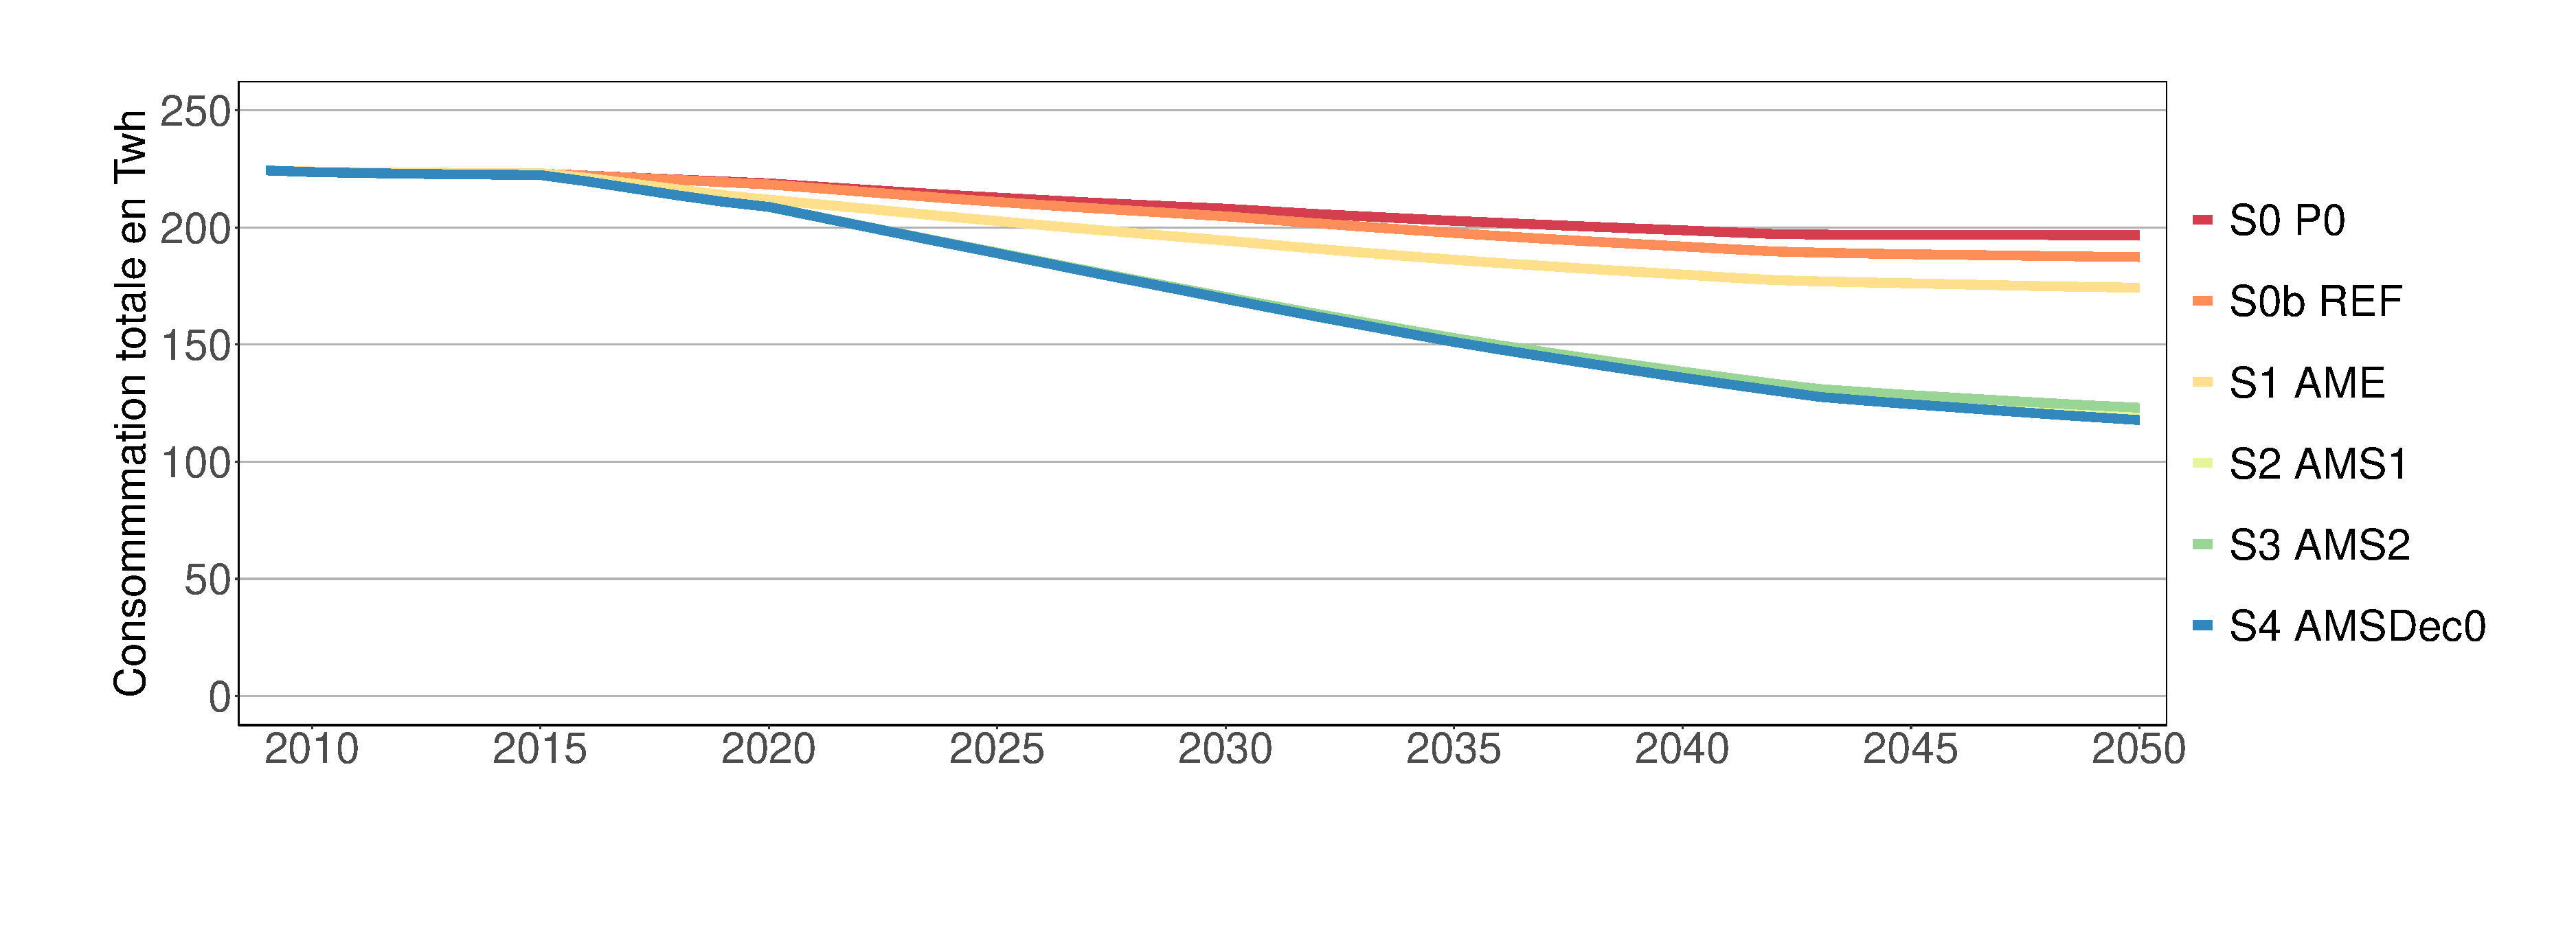
\includegraphics[width = 0.9\textwidth]{Evol_Conso_tot-1}  
\end{figure}


\begin{table}[h!] \caption{Evolution des consommations totales}
\centering 
\begin{tabular}[c]{|l|c|c|c|c|c|}
\hline
				& 		2015-2030  &	2015-2050 \\
\hline
P0  		&		-6.7~\% 	&-11.8~\% \\
REF  		&		-8.2~\% 	&-16~\% \\
AME  		&		-12.9~\%  &-21.9~\% \\
AMS1  	&		-23.5~\%  &-45.5~\% \\
AMS2  	&		-23.4~\%  &-44.7~\% \\
AMSDec0 & 	-23.8~\%  &-47~\% \\
\hline
\end{tabular}
\end{table}

Les consommations de chauffage baissent de 37~\% entre 2015 et 2050  de façon \og~autonome~\fg du fait du renouvellement des systèmes de chauffage, de la hausse des prix des énergies du fait du contexte macro-économique, de l’entrée progressive de bâtiments neufs performants et de la prise en compte de l’adaptation au changement climatique (scénario « REF »). Les mesures AME et AMS permettent d'atteindre les derniers gisements d’économie d’énergie plus coûteux et de réduire les consommations de chauffage de presque 70~\% entre 2015 et 2050 dans le cas du scénario \og~AMSDec0~\fg.

\begin{figure}[h!]
\centering 
\caption{Evolution des consommations de chauffage}\label{Evol_Conso_chauffage-1}  
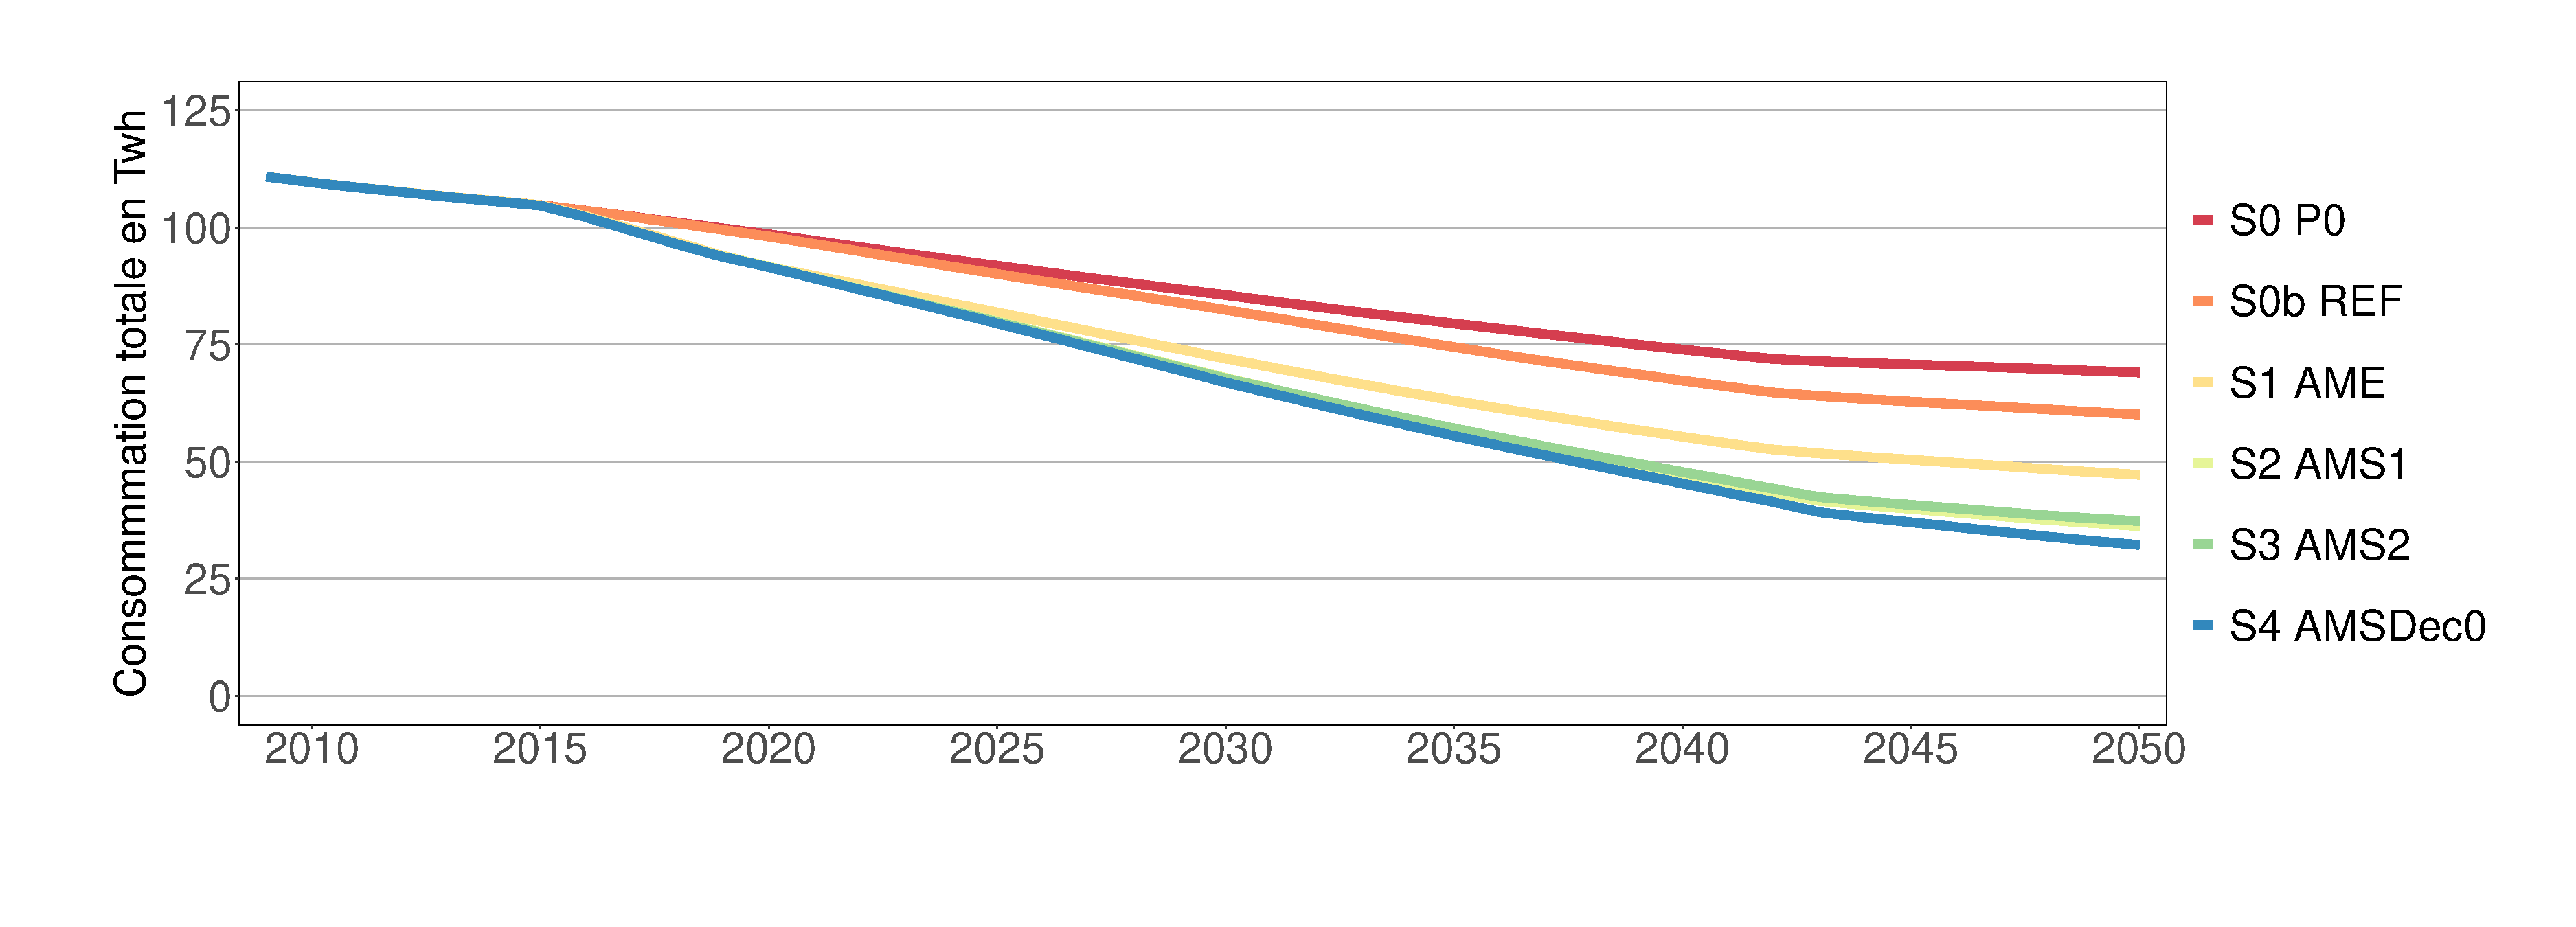
\includegraphics[width = 0.9\textwidth]{Evol_Conso_chauffage-1}  
\end{figure}

\begin{table}[h!] \caption{Evolution des consommations de chauffage}
\centering
\begin{tabular}[c]{|l|c|c|c|c|c|}
\hline
				& 	2015-2030  &2015-2050 \\
				\hline
P0  		&		-18.3~\%  & 	-34.1~\% \\
REF  		&		-21.4~\% 	& -42.7~\% \\
AME  		&		-31.3~\%  & -55~\% \\
AMS1  	&		-35.2~\%  & -65.4~\% \\
AMS2  	&		-35.3~\%  & -64.3~\% \\
AMSDec0 & 	-36.1~\%  & -69.2~\% \\
\hline
\end{tabular}
\end{table}

\clearpage

\subsubsection{Évolution des émissions totales et de chauffage}

Les émissions de CO$_2$ baissent de 43~\% dans le scénario AME du fait principalement de la baisse des émissions liées au chauffage (-61~\%). le scénario \og~AMSDec0~\fg montre que les mesures supplémentaires des scénarios AMS permettent de réduire les émissions de 25 points supplémentaires sans décarboner le mix énergétique. Pour réduire drastiquement les émissions, la décarbonation des mix énergétiques est nécessaire (scénarios AMS1 et AMS2). 


\begin{figure}[h!]
\centering
\caption{Evolution des émssions totales} \label{Evol_Em_tot-1}  
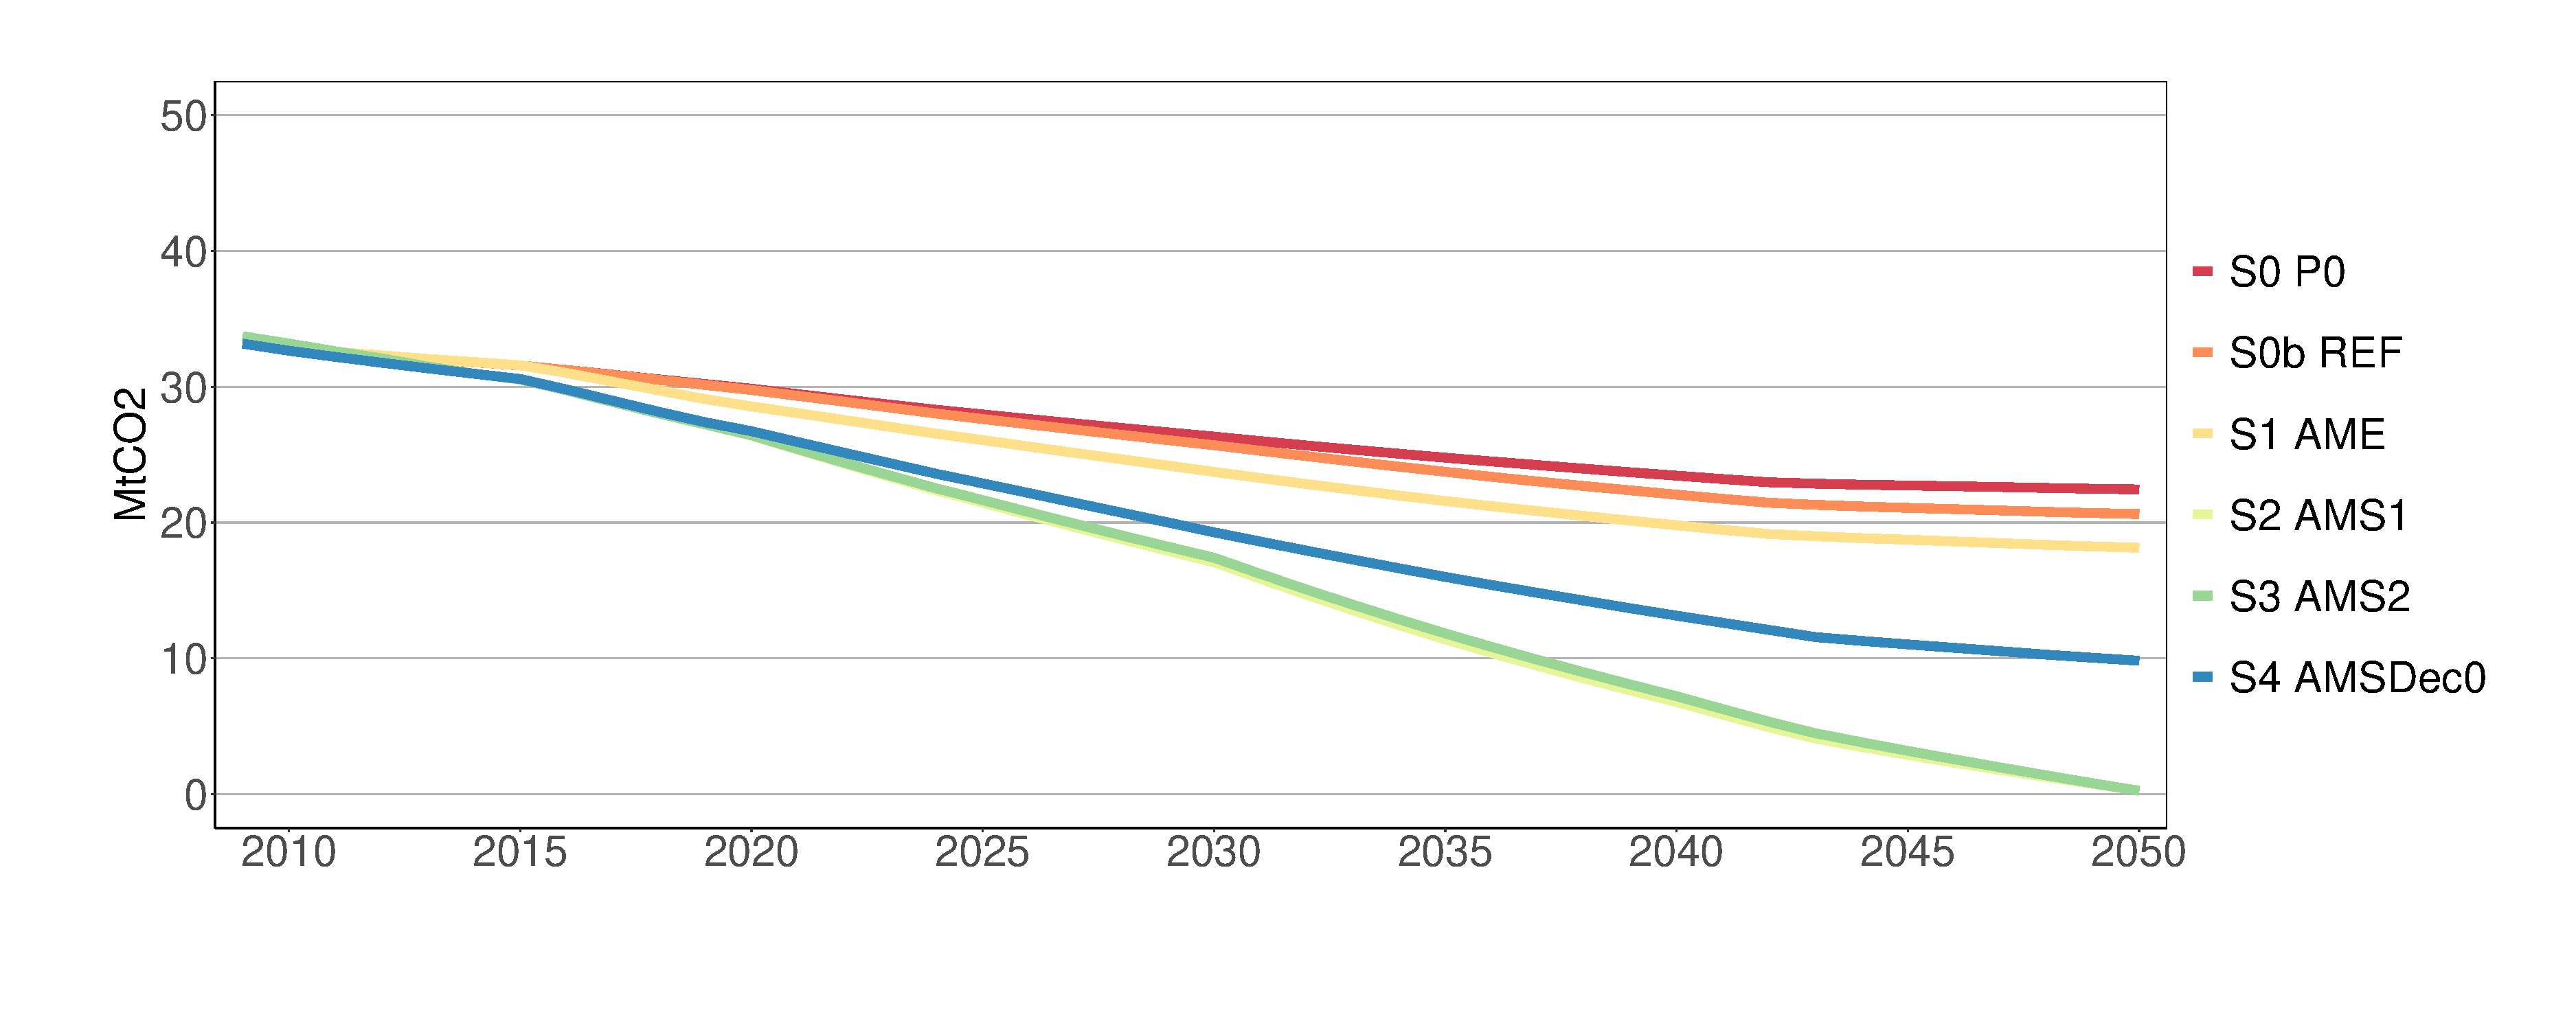
\includegraphics[width = 0.9\textwidth]{Evol_Em_tot-1}  
\end{figure}

Les mesures des scénarios AMS permettent d'abaisser le niveau des émissions de CO$_2$ plus rapidement, le niveau d'émission de 2050 du scénario AME est par exemplet atteint en 2030 pour les scénarios AMS1 et AMS2. Cela permet de diviser par 2 les émissions cumulées entre 2015 et 2060\footnote{on prolonge les émissions de 2050 de 10 ans pour tenir compte des gains apportées par les rénovations en fin de période} qui passent de 1000 MtCO$_2$ pour le scénario AME à un peu de 500 MtCO$_2$ pour les scénarios AMS1 et AMS2. Sans décarboner le mix énergétique, les mesures AMS permettent de diminuer de 25\% les émissions de CO$_2$ entre 2015 et 2060.  

\begin{table}[h!] \caption{Evolution des émissions de CO$_2$ totales}
\centering
\begin{tabular}[c]{|l|c|c|c|c|c|}
\hline
				& 	2015-2030  &2015-2050 \\
				\hline
P0  		&		-16.6~\%  & -28.9~\% \\
REF  		&		-18.6~\% 	& -34.7~\% \\
AME  		&		-24.9~\%  & -42.5~\% \\
AMS1  	&		-44.1~\%  & -99.1~\% \\
AMS2  	&		-43~\%  	& -99.2~\% \\
AMSDec0 & 	-36.9~\%  & -67.8~\% \\
\hline
\end{tabular}
\end{table}

\begin{table}[h!] \caption{Emissions de CO$_2$ cumulées entre 2015 et 2060 (MtCO$_2$)}
\centering
\begin{tabular}[c]{|l|c|c|c|c|c|}
\hline
				& Emissions cumulées (MtCO$_2$) \\
\hline				
P0 			& 1~139 \\
REF 		& 1~091 \\
AME 		& 1~004 \\
AMS1 		& 523 \\
AMS2 		& 531 \\
AMSDec0 & 753 \\
\hline
\end{tabular}
\end{table}


\begin{figure}[h!]
\centering 
\caption{Evolution des émissions liées au chauffage}\label{Evol_Em_Chauff-1}  
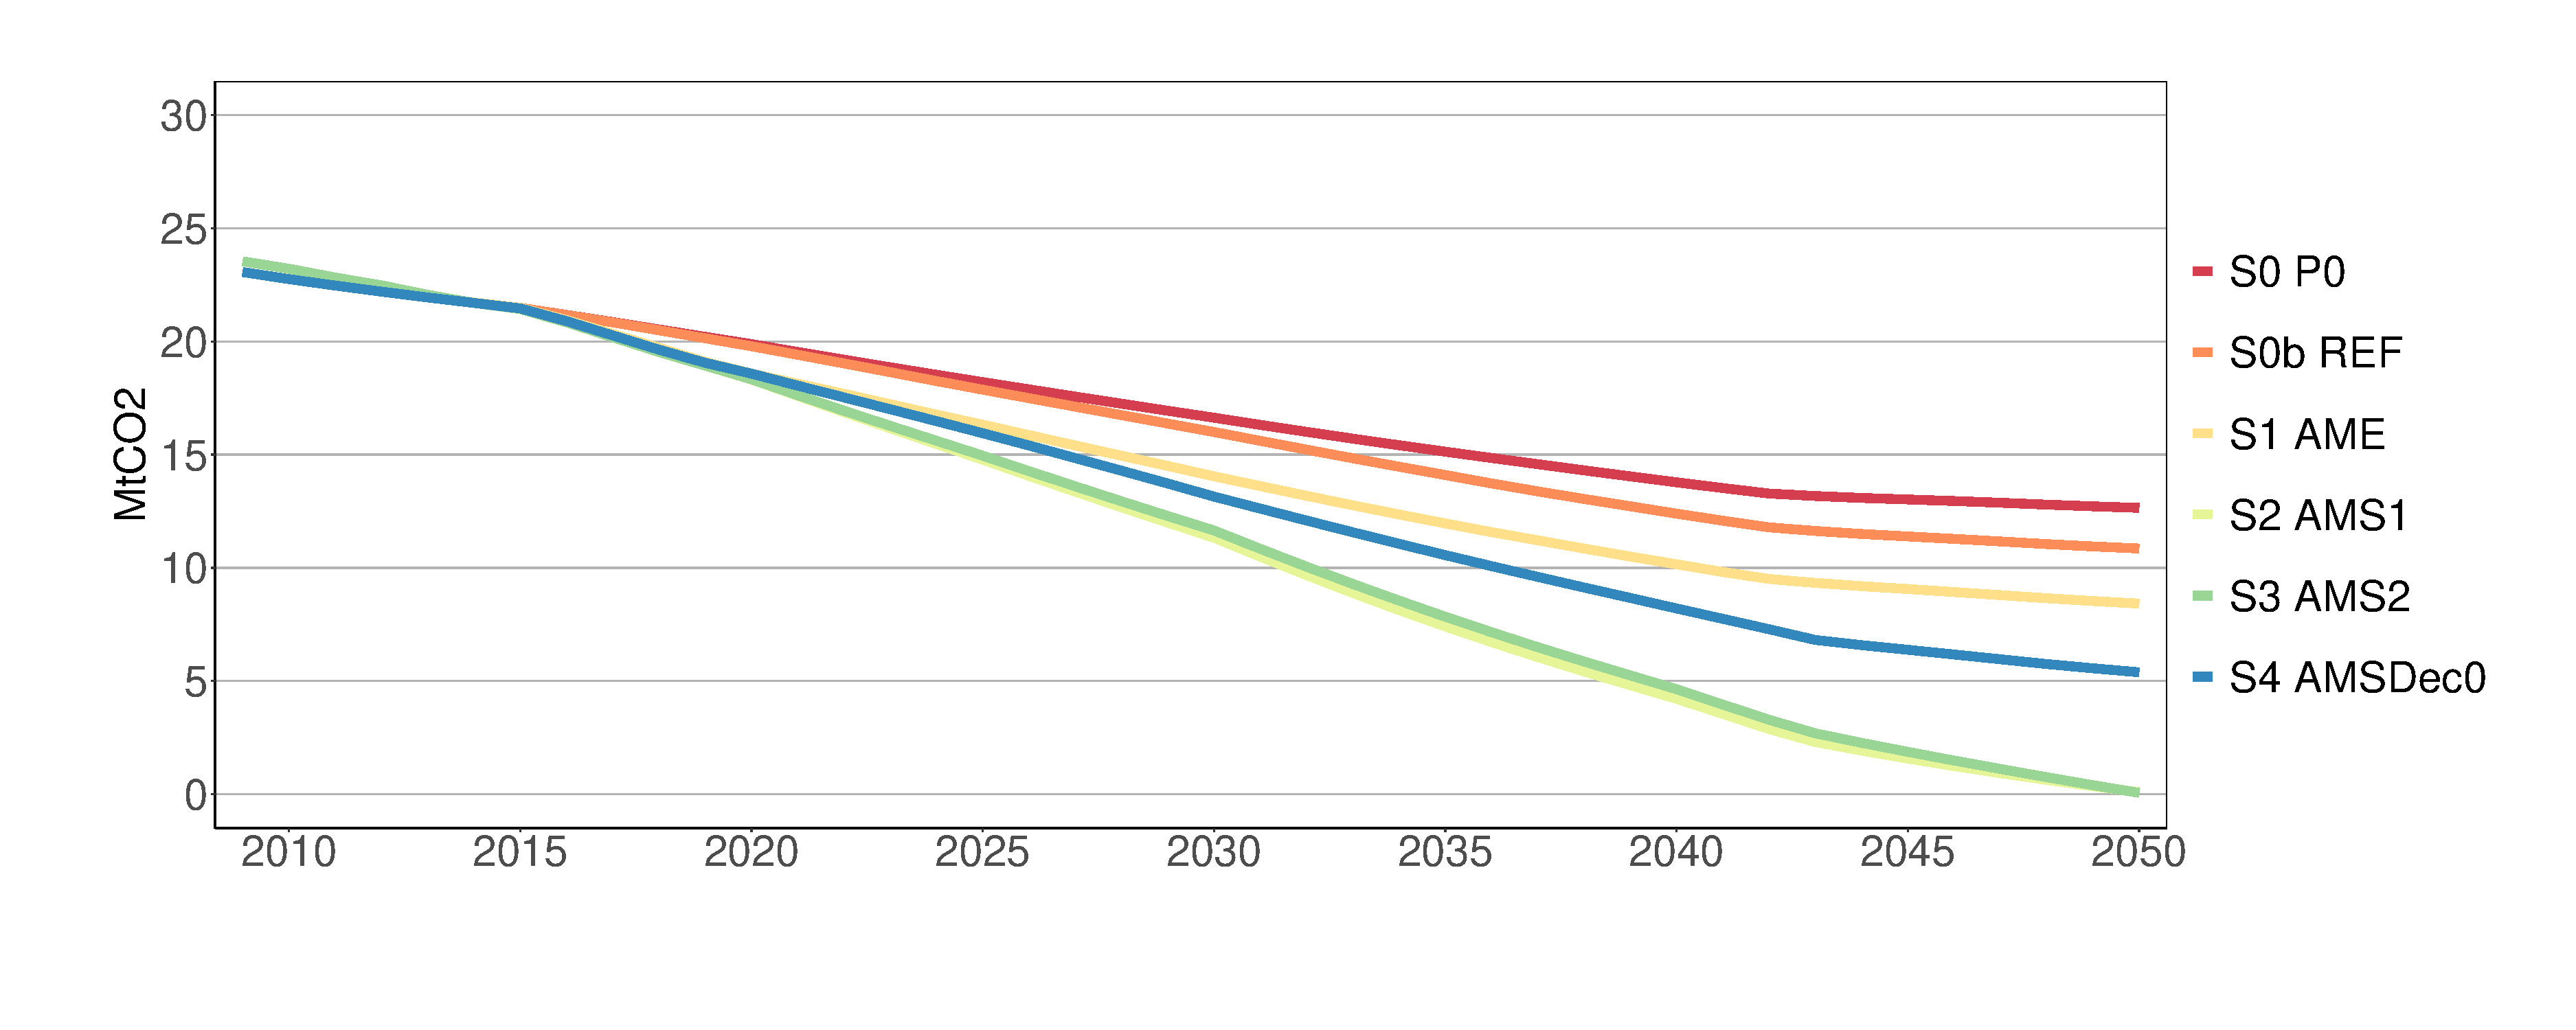
\includegraphics[width = 0.9\textwidth]{Evol_Em_Chauff-1}  
\end{figure}

\clearpage

\subsection{Résultats détaillés}

Dire que l'on se concentre sur le chauffage car c'est la partie endogène du modèle et sa vraie plus-value. 
D'autre part le modèle est plus pertinent sur le parc existant car les investissements sur le neuf ne sont pas comptabilisés 

\subsubsection{Évolution des consommations unitaires par branche}

Les consommations unitaires du parc tertiaire pour l'ensemble des usages passent de 231 à 150 kWh par m² par an pour le scénario AME (-35~\%), cette baisse étant principalement due à la baisse des consommations unitaires de chauffage (figure \ref{Conso_u_branche_2050-1}). Dans le scénario AMSDec, les consommations unitaires pour les autres usages diminuent aussi significativement notamment l'ECS et l'éclairage. La consommation unitaire moyenne passe à 104 kWh par m² par an (-55~\%). L'ensemble des branches est impacté par les rénovations même si les consommations unitaires de certaines diminuent plus fortement en pourcentage (figure \ref{Conso_u_branche_2050-1}).  

REGARDER si on prend seulement les usages RT et comparer à BBC rénovation dans le résidentiel. 


\begin{figure}[h!]
\centering 
\caption{Evolution des consommations unitaires par branche entre 2015 et 2050}\label{Conso_u_branche_2050-1}  
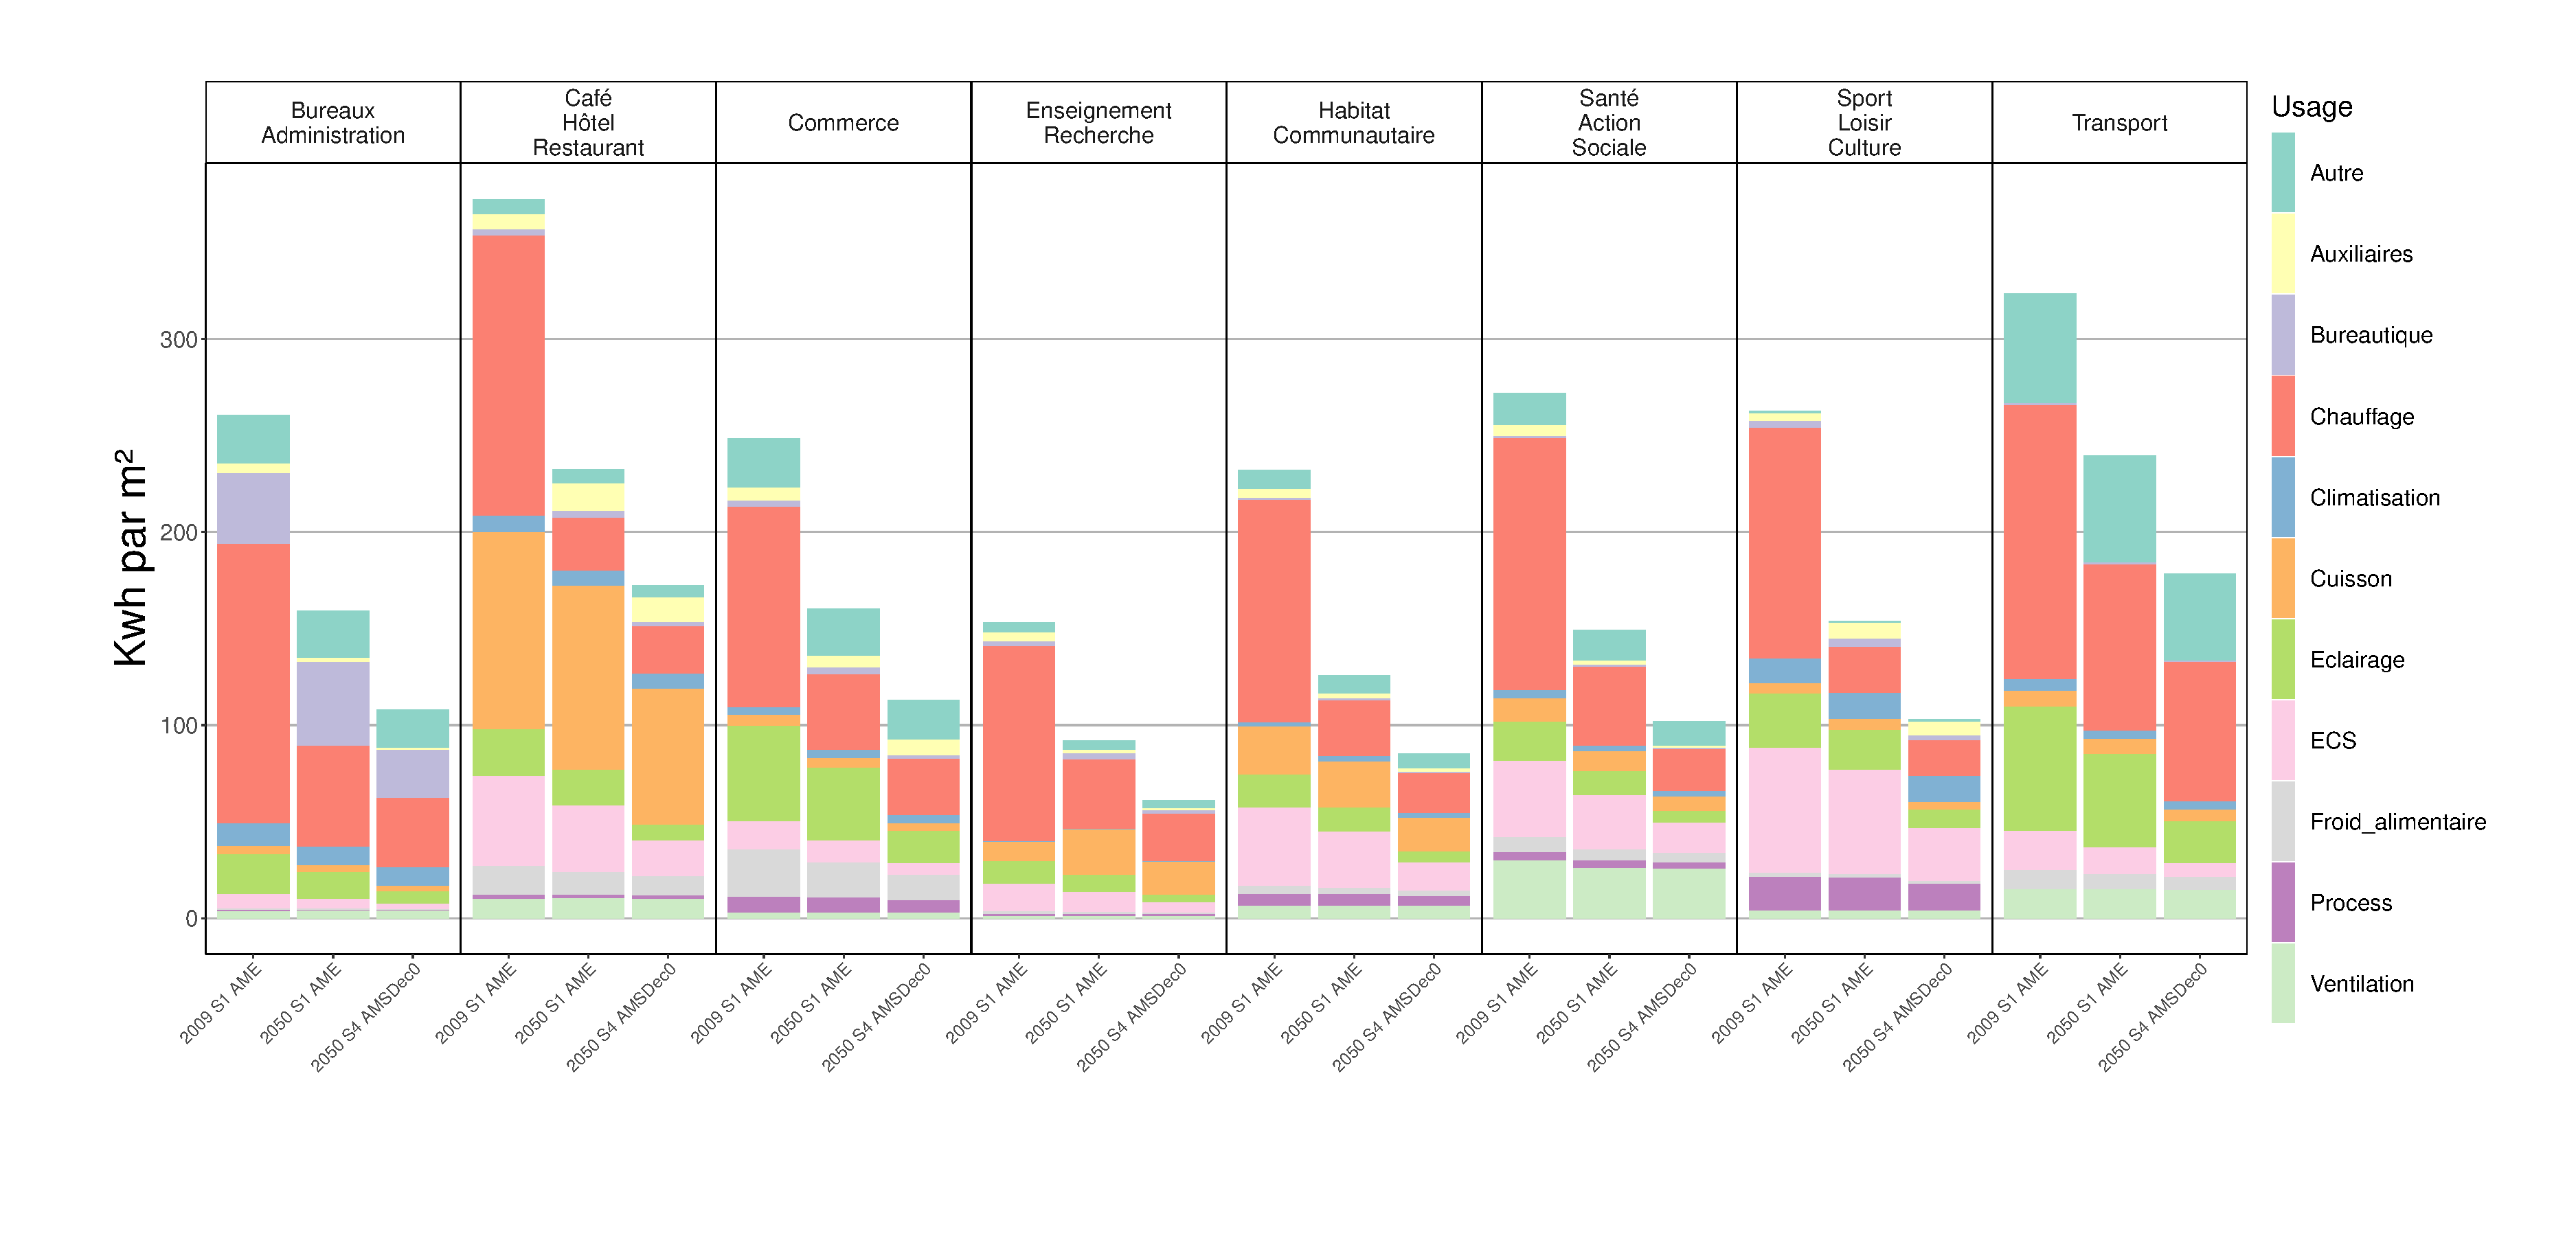
\includegraphics[width = 0.9\textwidth]{Conso_u_branche_2050-1}  
\end{figure}


\subsubsection{Évolution des consommations unitaires de chauffage}

Les consommations de chauffage de presque 70~\% entre 2015 et 2050 dans le scénario \og~AMSDec0~\fg. Cette baisse forte des consommations est la résultante de différents effets sur les consommations unitaires de chauffage du parc tertiaire qui sont résumés sur le graphique \ref{graph_consultant_consou} et dans le tableau \ref{decomp_conso_u}. En comparant les consommations unitaires du parc existant en 2015 et en 2050 pour le scénario P0 (sans mesures, prix constants), on observe une baisse de 32~\% ce qui montre qu'une part importante de la baisse des consommations se fait de manière \og~ autonome~\fg. En effet, le modèle est calibré pour maintenir un niveau tendanciel de rénovation sur le bâti  (un peu moins de 1~\% du parc par an) et un rythme de renouvellement des systèmes de chauffage de 3~\% par an. En 2050, environ 30~\% du parc aura connu au moins une rénovation du bâti. D'autre part, la prise en compte de l'adaptation au changement climatique dans le modèle conduit à une baisse du besoin unitaire de chauffage de 5,3~\% entre 2015 et 2050 du fait de température extérieure plus élevée. Ces deux élements entraînent au total une baisse de 16~\% du besoin unitaire de chauffage des bâtiments du parc. Entre 2015 et 2050, l'intégralité des systèmes de chauffage aura été renouvelé ce qui entraîne une hausse de 24~\% des rendements moyens des systèmes. Ces rénovations dites \og~ autonomes~\fg incluent en réalité l'effet des précédentes réglementations thermiques sur les bâtiments existants notamment celles imposant un niveau d'exigence minimum aux matériaux utilisés pour l'isolation et aux systèmes de chauffage vendus (RT élément par élement, RT globale...). Ces réglementations mettent un certain temps à se propager dans le parc existant mais en 2050 elles sont largement répandues ce qui affectent sensiblement les consommations de chauffage. 

\begin{figure}[h!]
\centering 
\caption{Décomposition de l'effet des scénarios et des mesures sur les consommations unitaires de chauffage}\label{graph_consultant_consou}  
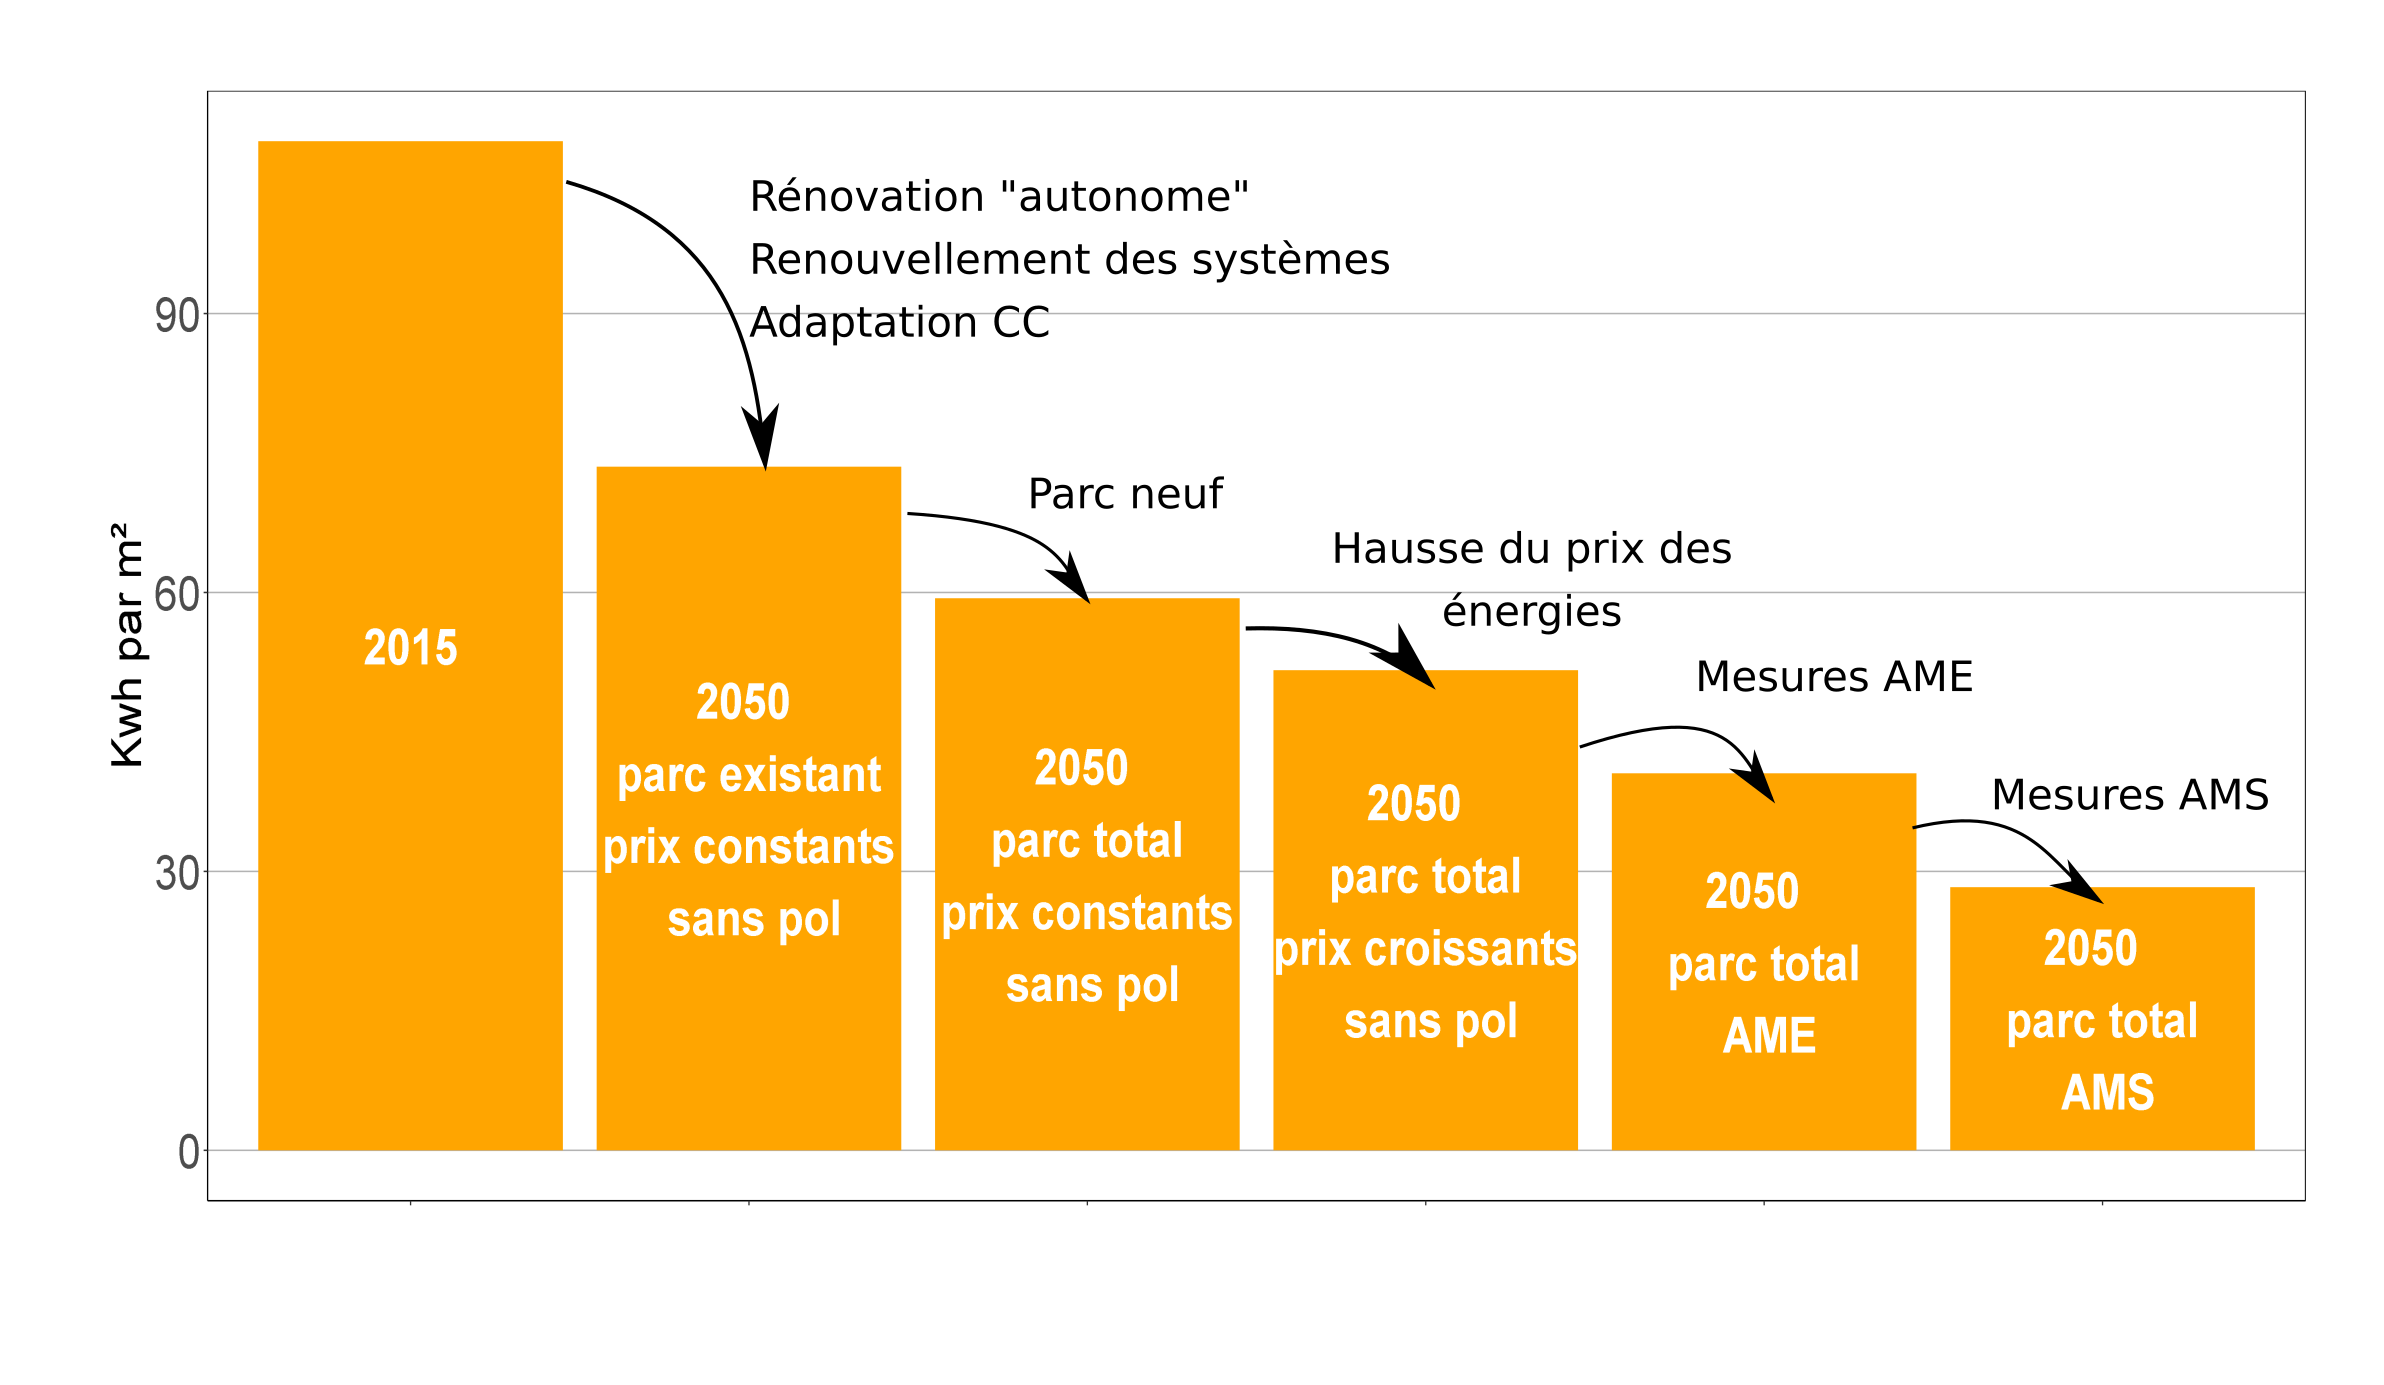
\includegraphics[width = 0.9\textwidth]{graph_consultant_consou}  
\end{figure}
 
Sous l'effet de la pénétration de bâtiments entrants remplaçant en partie les bâtiments existants, la consommation unitaire de chauffage du parc tertiaire total baisse de 14 points supplémentaires dans le scénario \og~AMSDec0~\fg. Ici encore, la baisse des consommations est due en partie à la réglementation thermique dans les bâtiments neufs (RT 2012) ainsi qu'au réglementation thermiques précédentes qui imposent des niveaux de consommations unitaires plus basses aux bâtiments entrants par rapport aux bâtiments existants qui sortent du parc. D'autre part la plupart des systèmes de chauffage dans les bâtiments neufs sont performants avec des rendements élevés.   

En comparant les consommations unitaires de chauffage de l'ensemble du parc en 2050 du scénario P0 et du scénario REF, on observe l'impact de la hausse du prix des énergies du fait du contexte macro-économique prix en hypothèse. C'est en effet la seule variable qui est ajustée entre ces deux scénarios. La hausse des prix entraîne une baisses des consommations unitaires de 6 points supplémentaires avec un impact surtout sur les rénovations du bâti.  

La comparaison avec les consommations unitaires de chauffage de l'ensemble du parc en 2050 pour les scénarios AME et AMSDec0 donne enfin l'impact additionnels des mesures contenues dans ces deux scénarios. L'impact des mesures peut paraître limité (10 points supplémentaires pour les mesures AME et 23 points supplémentaires pour les mesures AMS) mais cela provient du fait que les mesures AME et AMS arrivent en « bout de course » pour atteindre les derniers gisements d’économie d’énergie, c'est à dire les plus coûteux. Ces gisements permettent de diviser par 4 les consommations unitaires de chauffage à horizon 2050. 

\begin{table}[h] \caption{Décomposition de l'effet des scénarios et des mesures sur les consommations unitaires de chauffage}\label{decomp_conso_u}
\centering
\scriptsize
\begin{tabular}[c]{|l|c|c|c|c|c|c|}
\hline
																						& 	2015  		&	2050 						& 2050 						& 2050 						& 2050 						& 2050				\\
																						& Parc total 	& Parc existant		& Parc total			&	Parc total			& Parc total      & Parc total	\\
																						& 						& Sans mesures		& Sans mesures		& Sans mesures		& mesures AME     & mesures AMS	\\
																						&							& prix constants	& prix constants	& prix croissants	& prix croissants & prix croissants\\ \hline
Scénario 																		& P0 					& P0							&	P0							&	REF							&	AME							& AMSDec0
\\ \hline
Consommation unitaire moyenne 							&		109  			& 74  (-32~\%)		&	59 (-46~\%)			& 52 (-52~\%)			& 41 (-62~\%)			& 28 (-75~\%) \\
 (kwh EF par m²)														&							&									&									&									&									&							\\
Besoin unitaire moyen (kwh EF par m²)				&		97 				& 82 (-16~\%)			& 68 (-30~\%)		  & 64 (-34~\%)			&	55 (-43~\%)			&	46 (-52~\%) \\
= Rénovation du bâti												&							&									&									&									&									&							\\
Rendement moyen															&		0,9 			&  1,1 (+24~\%) 	& 1,2 (+34~\%)  	& 1,2 (+34~\%) 		& 1,3 (+46~\%)		&	1,6 (+80~\%)\\
= changement des systèmes										&							&									&									&									&									&							\\
\hline
\end{tabular}
\end{table}

\clearpage

\subsubsection{Évolution du mix énergétique pour le chauffage}

Les évolutions des parts de marché surfaciques des systèmes de chauffage pour l’ensemble du parc tertiaire (neuf + existant) sont représentées dans le graphique \ref{Evol_PM_syst_all-1}. 

Ces évolutions montrent une progression des systèmes de chauffage performants notamment des PAC, des systèmes DRV et rooftop et des systèmes gaz performant. Les systèmes au fioul connaissent un fort recul dans tous les scénarios et disparaissent pratiquement dans les scénarios où la composante carbone est présente. Dans tous les scénarios AMS où la composante carbone est forte, on observe une progression de l’électricité dans les surfaces chauffées et un recul du gaz après 2030. Ceci est particulièrement marqué dans le scénario AMSDec0 où le prix du gaz augmente le plus fortement car la composante carbone s'applique à 100~\% sur son prix (pas de pénétration du biogaz). Le gaz ne représente plus que 25~\% des surfaces chauffées en 2050 dans ce scénario. Les surfaces chauffées par le chauffage urbain et le bois progresse assez peu sauf dans le scénario AMS1 où toutes les autres énergies que le bois voient leurs prix augmenter fortement. Les évolutions de la part de marché des énergies dans les consommations (figure \ref{Evol_PM_ener_cahuffage_exi-1}) montre des évolutions similaires.

\begin{figure}[h!]
\centering 
\caption{Évolution de la part de marché des systèmes de chauffage (part des surfaces)}\label{Evol_PM_syst_all-1}  
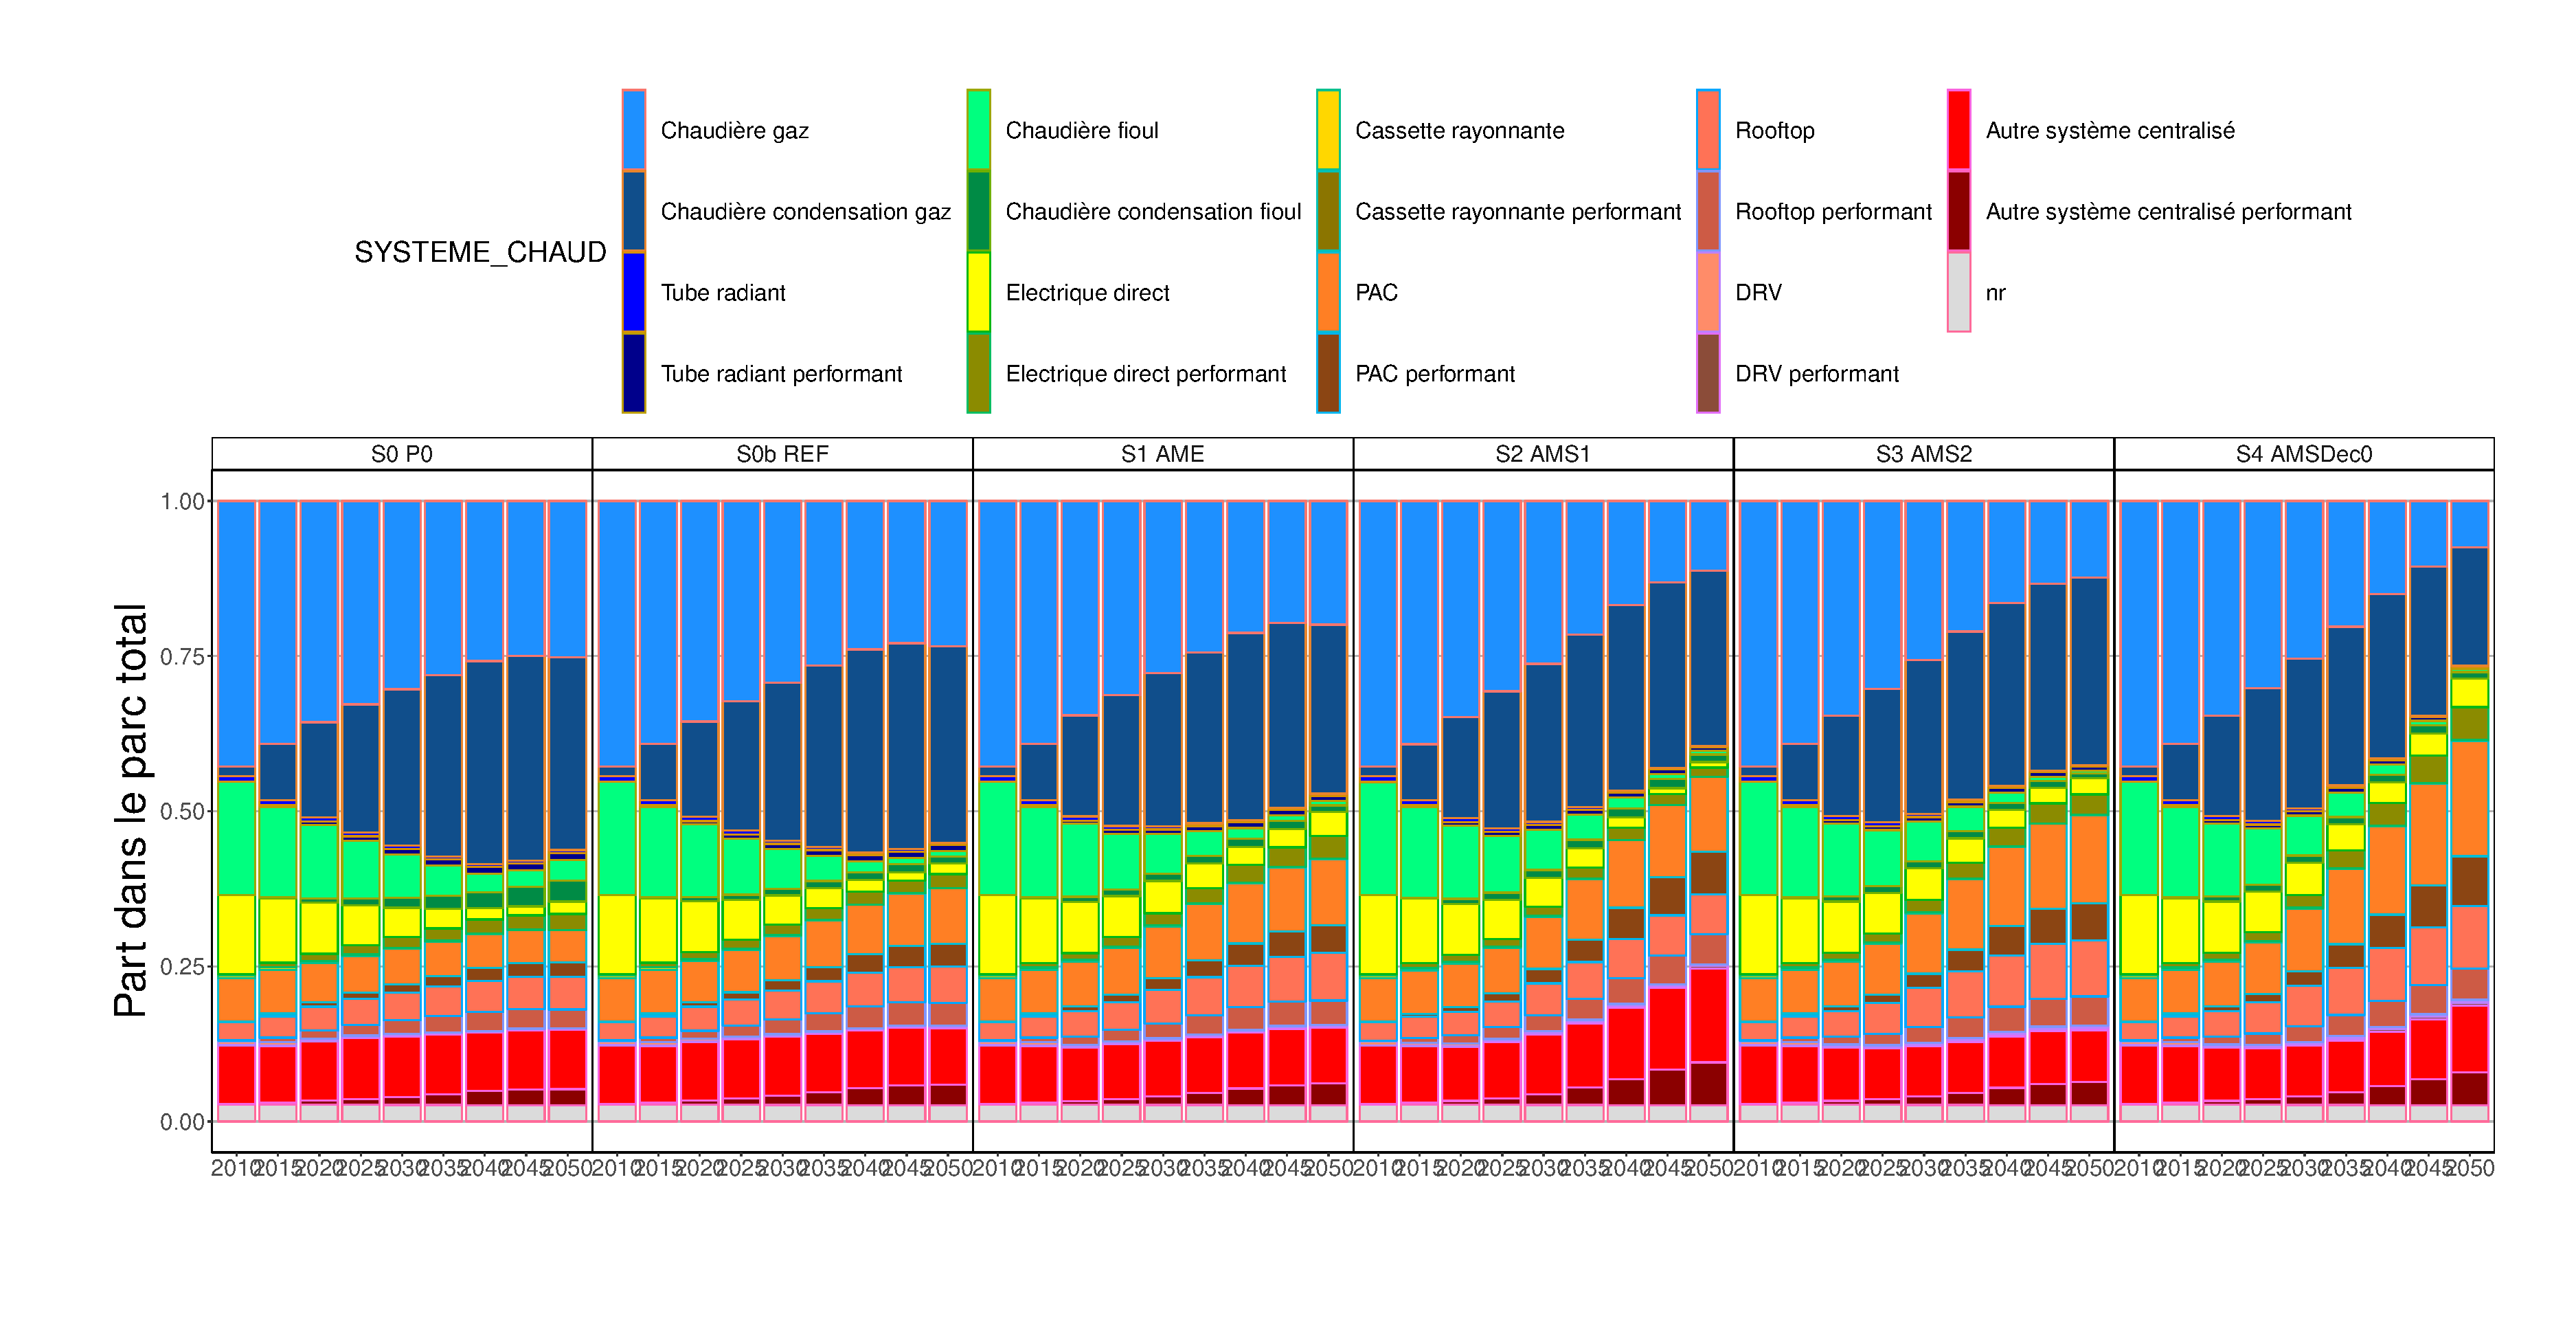
\includegraphics[width = 0.9\textwidth]{Evol_PM_syst_all-1}  
\end{figure}

\begin{figure}[h!]
\centering 
\caption{Évolution de la part de marché des énergies dans le chauffage du parc existant (part des consommations)}\label{Evol_PM_ener_cahuffage_exi-1}  
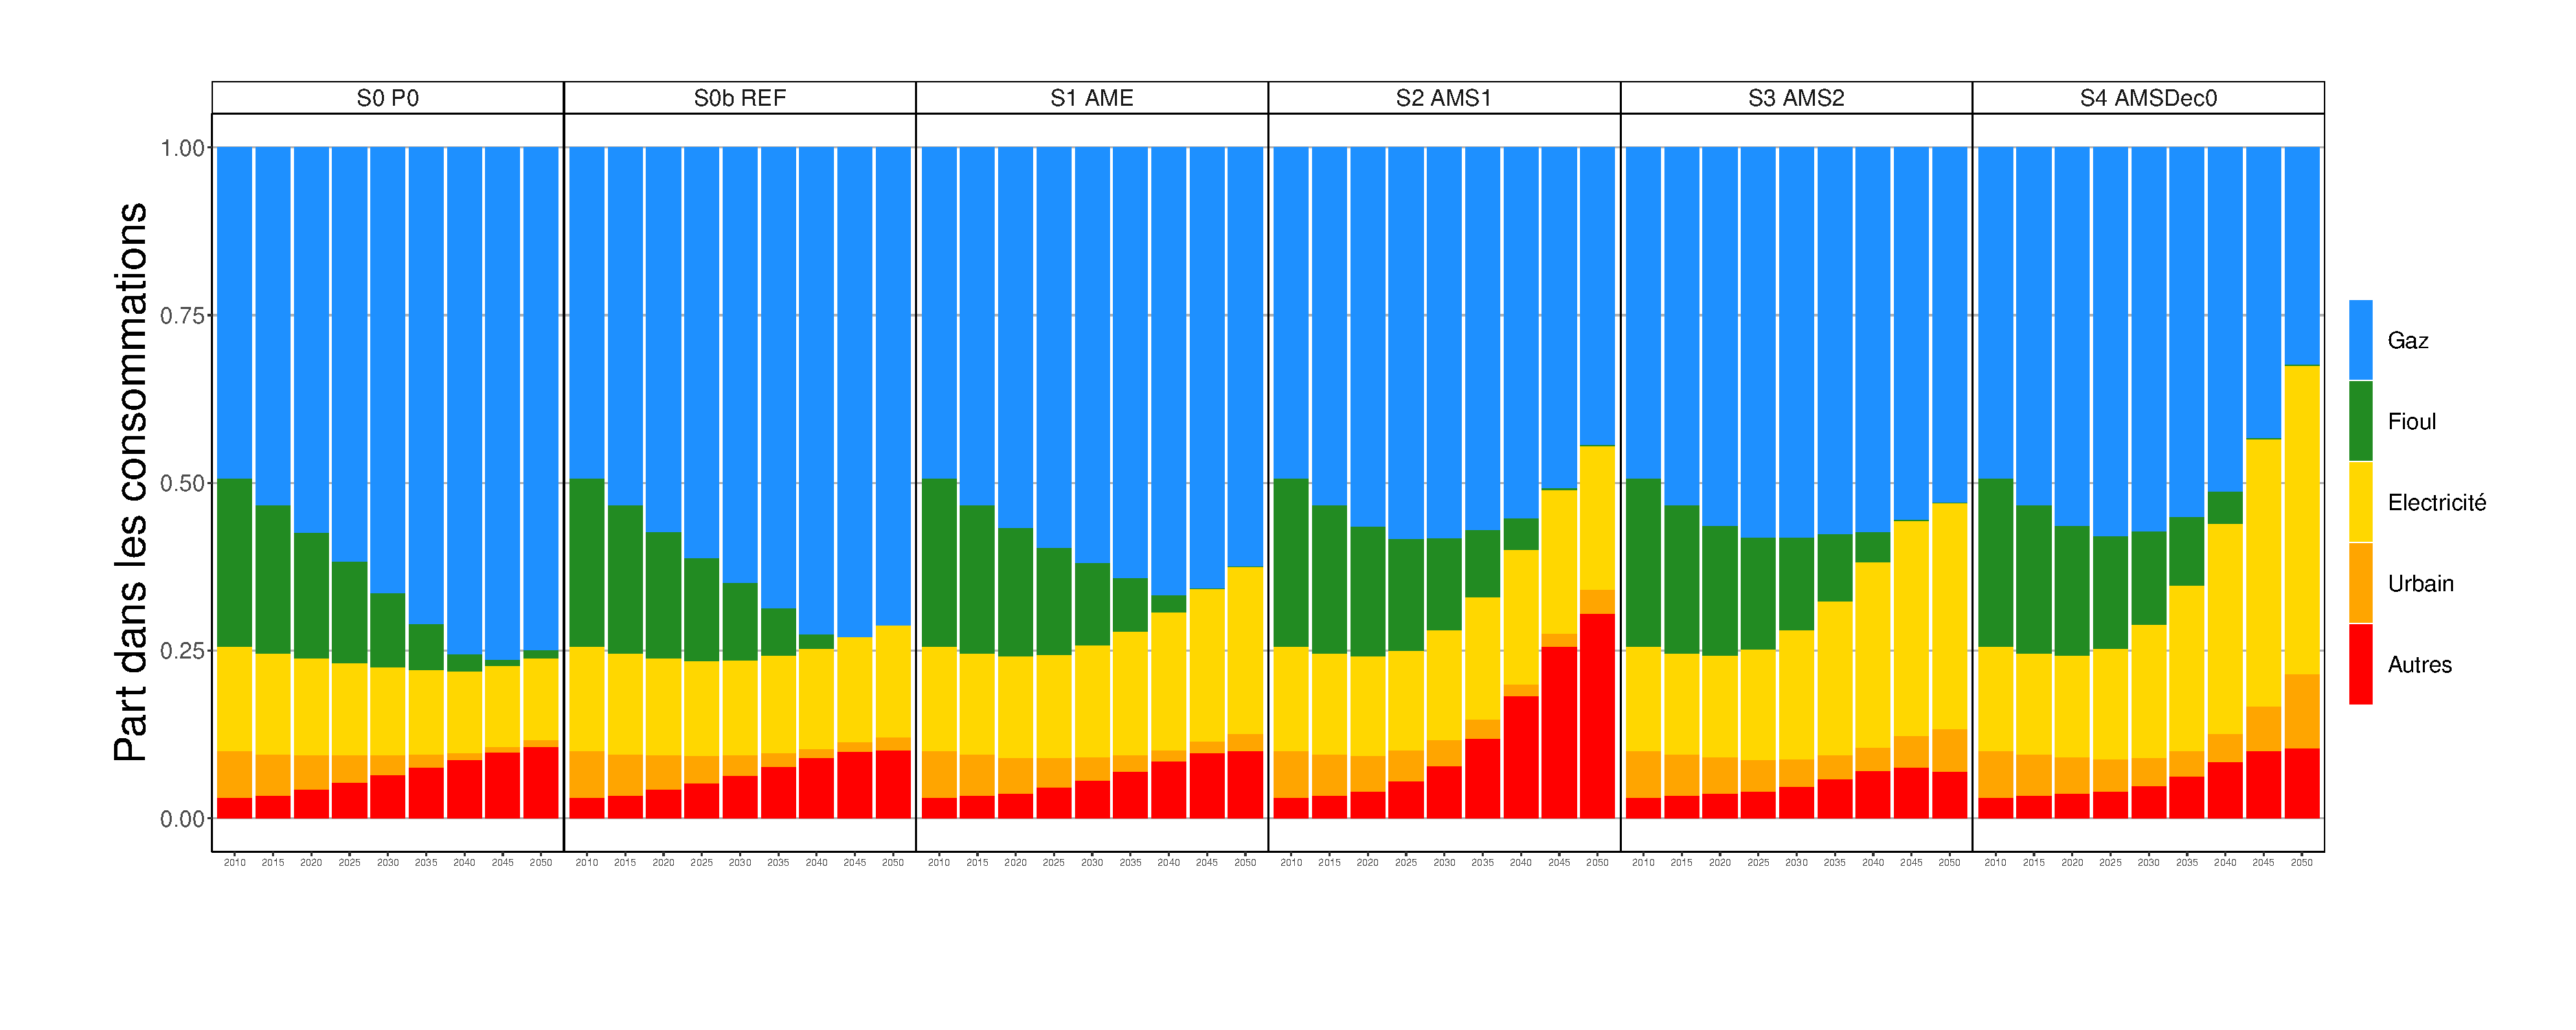
\includegraphics[width = 0.9\textwidth]{Evol_PM_ener_cahuffage_exi-1}  
\end{figure}


\begin{figure}[ht!]
\centering 
\caption{Evolution des émissions liées au chauffage par énergie}\label{Evol_Em_energie_chauffage-1}  
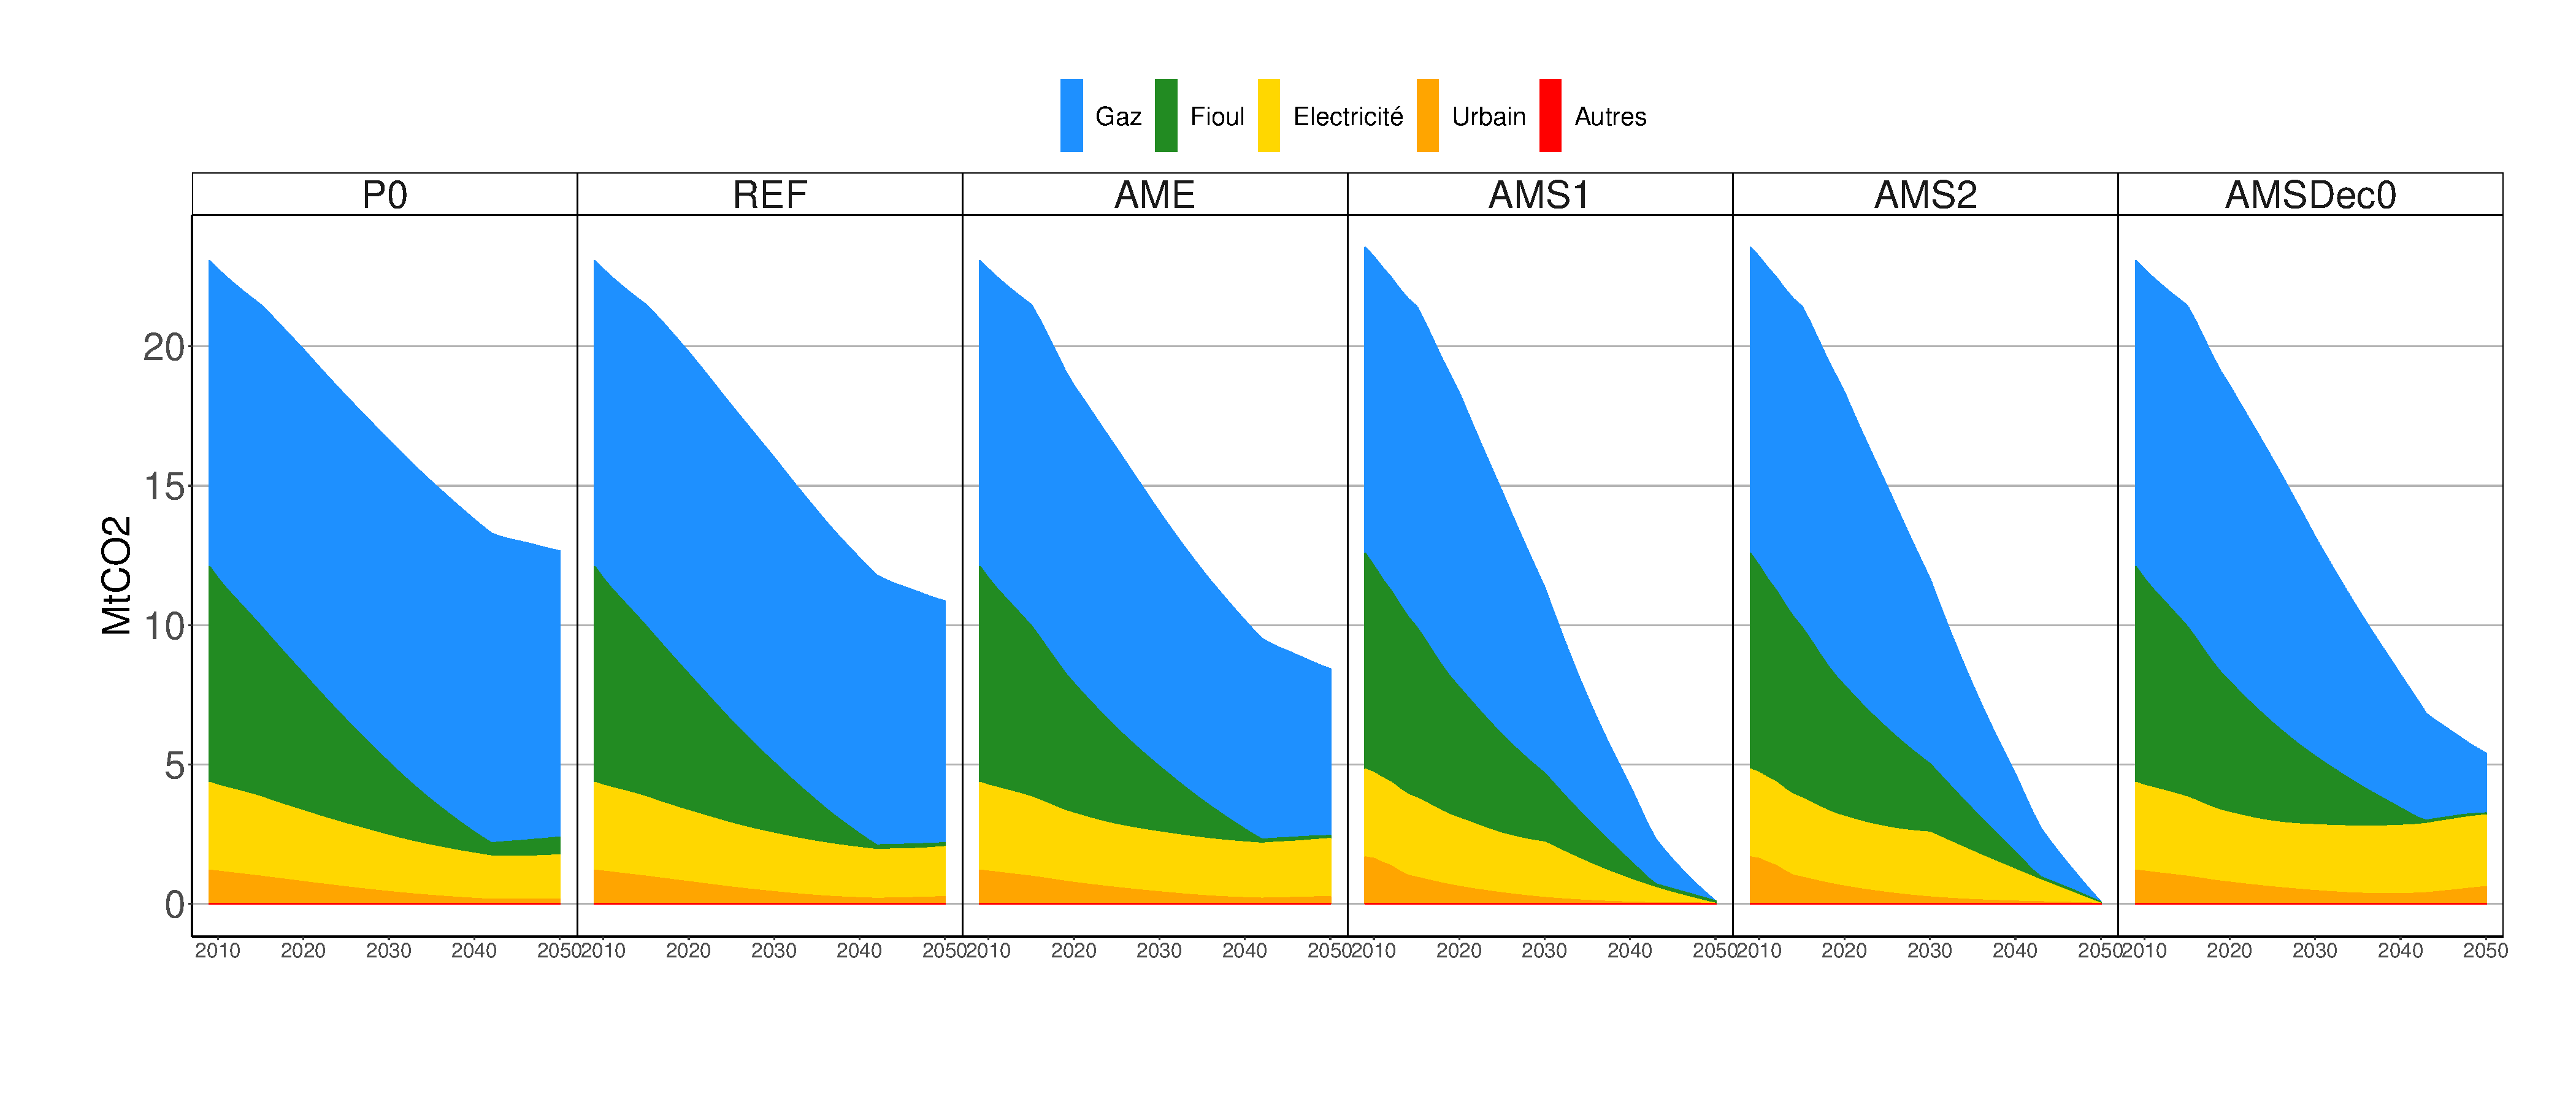
\includegraphics[width = 0.9\textwidth]{Evol_Em_energie_chauffage-1}  
\end{figure}

\clearpage

\subsubsection{Investissements dans la rénovation du bâti et les changements de systèmes de chauffage}

Les flux d'investissements (non actualisés) par type de geste et par système de chauffage sont représentés sur les graphiques ci-dessous (figures \ref{INV_Gestes-1} et \ref{INV_syst-1}). Ces investissements ne concerne que la partie isolation de l'enveloppe de bâtiments et les systèmes de chauffage, pas les investissements liés aux changements des systèmes d'ECS, d'éclairage, ou de climatisation. 

Dans les scénarios AME et AMS, la hausse importante de l'investissement dans la rénovation entre après 2015, en comparaison avec les scénarios sans mesures, est principalement liée au dispositif des CEE et aux obligations de rénovation (travaux embarqués, Patrimoine immobilier de l’Etat, décret tertiaire). 
Le scénario AME conduit les usagers des bâtiments à investir 78 milliards d’euros entre 2015 et 2050 soit 27 milliards d'euros supplémentaires par rapport à un scénario sans les mesures de l'AME (REF), soit une hausse de ~\% des investissements dans la rénovation. Les mesures du scénario AMS induisent entre 20 et 28 milliards d’euros d’investissement supplémentaires par rapport au scénario AME. Les investissements additionnels engendrés par les mesures AMS concernent surtout sur les gestes sur bâti. D'autre part, les investissements combinant rénovations et changement de système de chauffage sont deux fois plus importants dans les scénarios AMS (12 milliards d’euros contre 6 milliards d’euros pour le scénario AME). Enfin, les investissements de niveau BBC progressent significativement dans les scénarios AMS par rapport au scénario AME. Les scénarios AMS1 et AMSDec0 induisent 10 milliards d'euros d'investissements additionnels en comparaison avec le scénario AMS2 où les prix des énergies sont plus faibles car la décarbonation des énergies est fortement subventionnée par l’État.

\begin{figure}[h!]
\centering 
\caption{Investissements dans la rénovation du bâti}\label{INV_Gestes-1}  
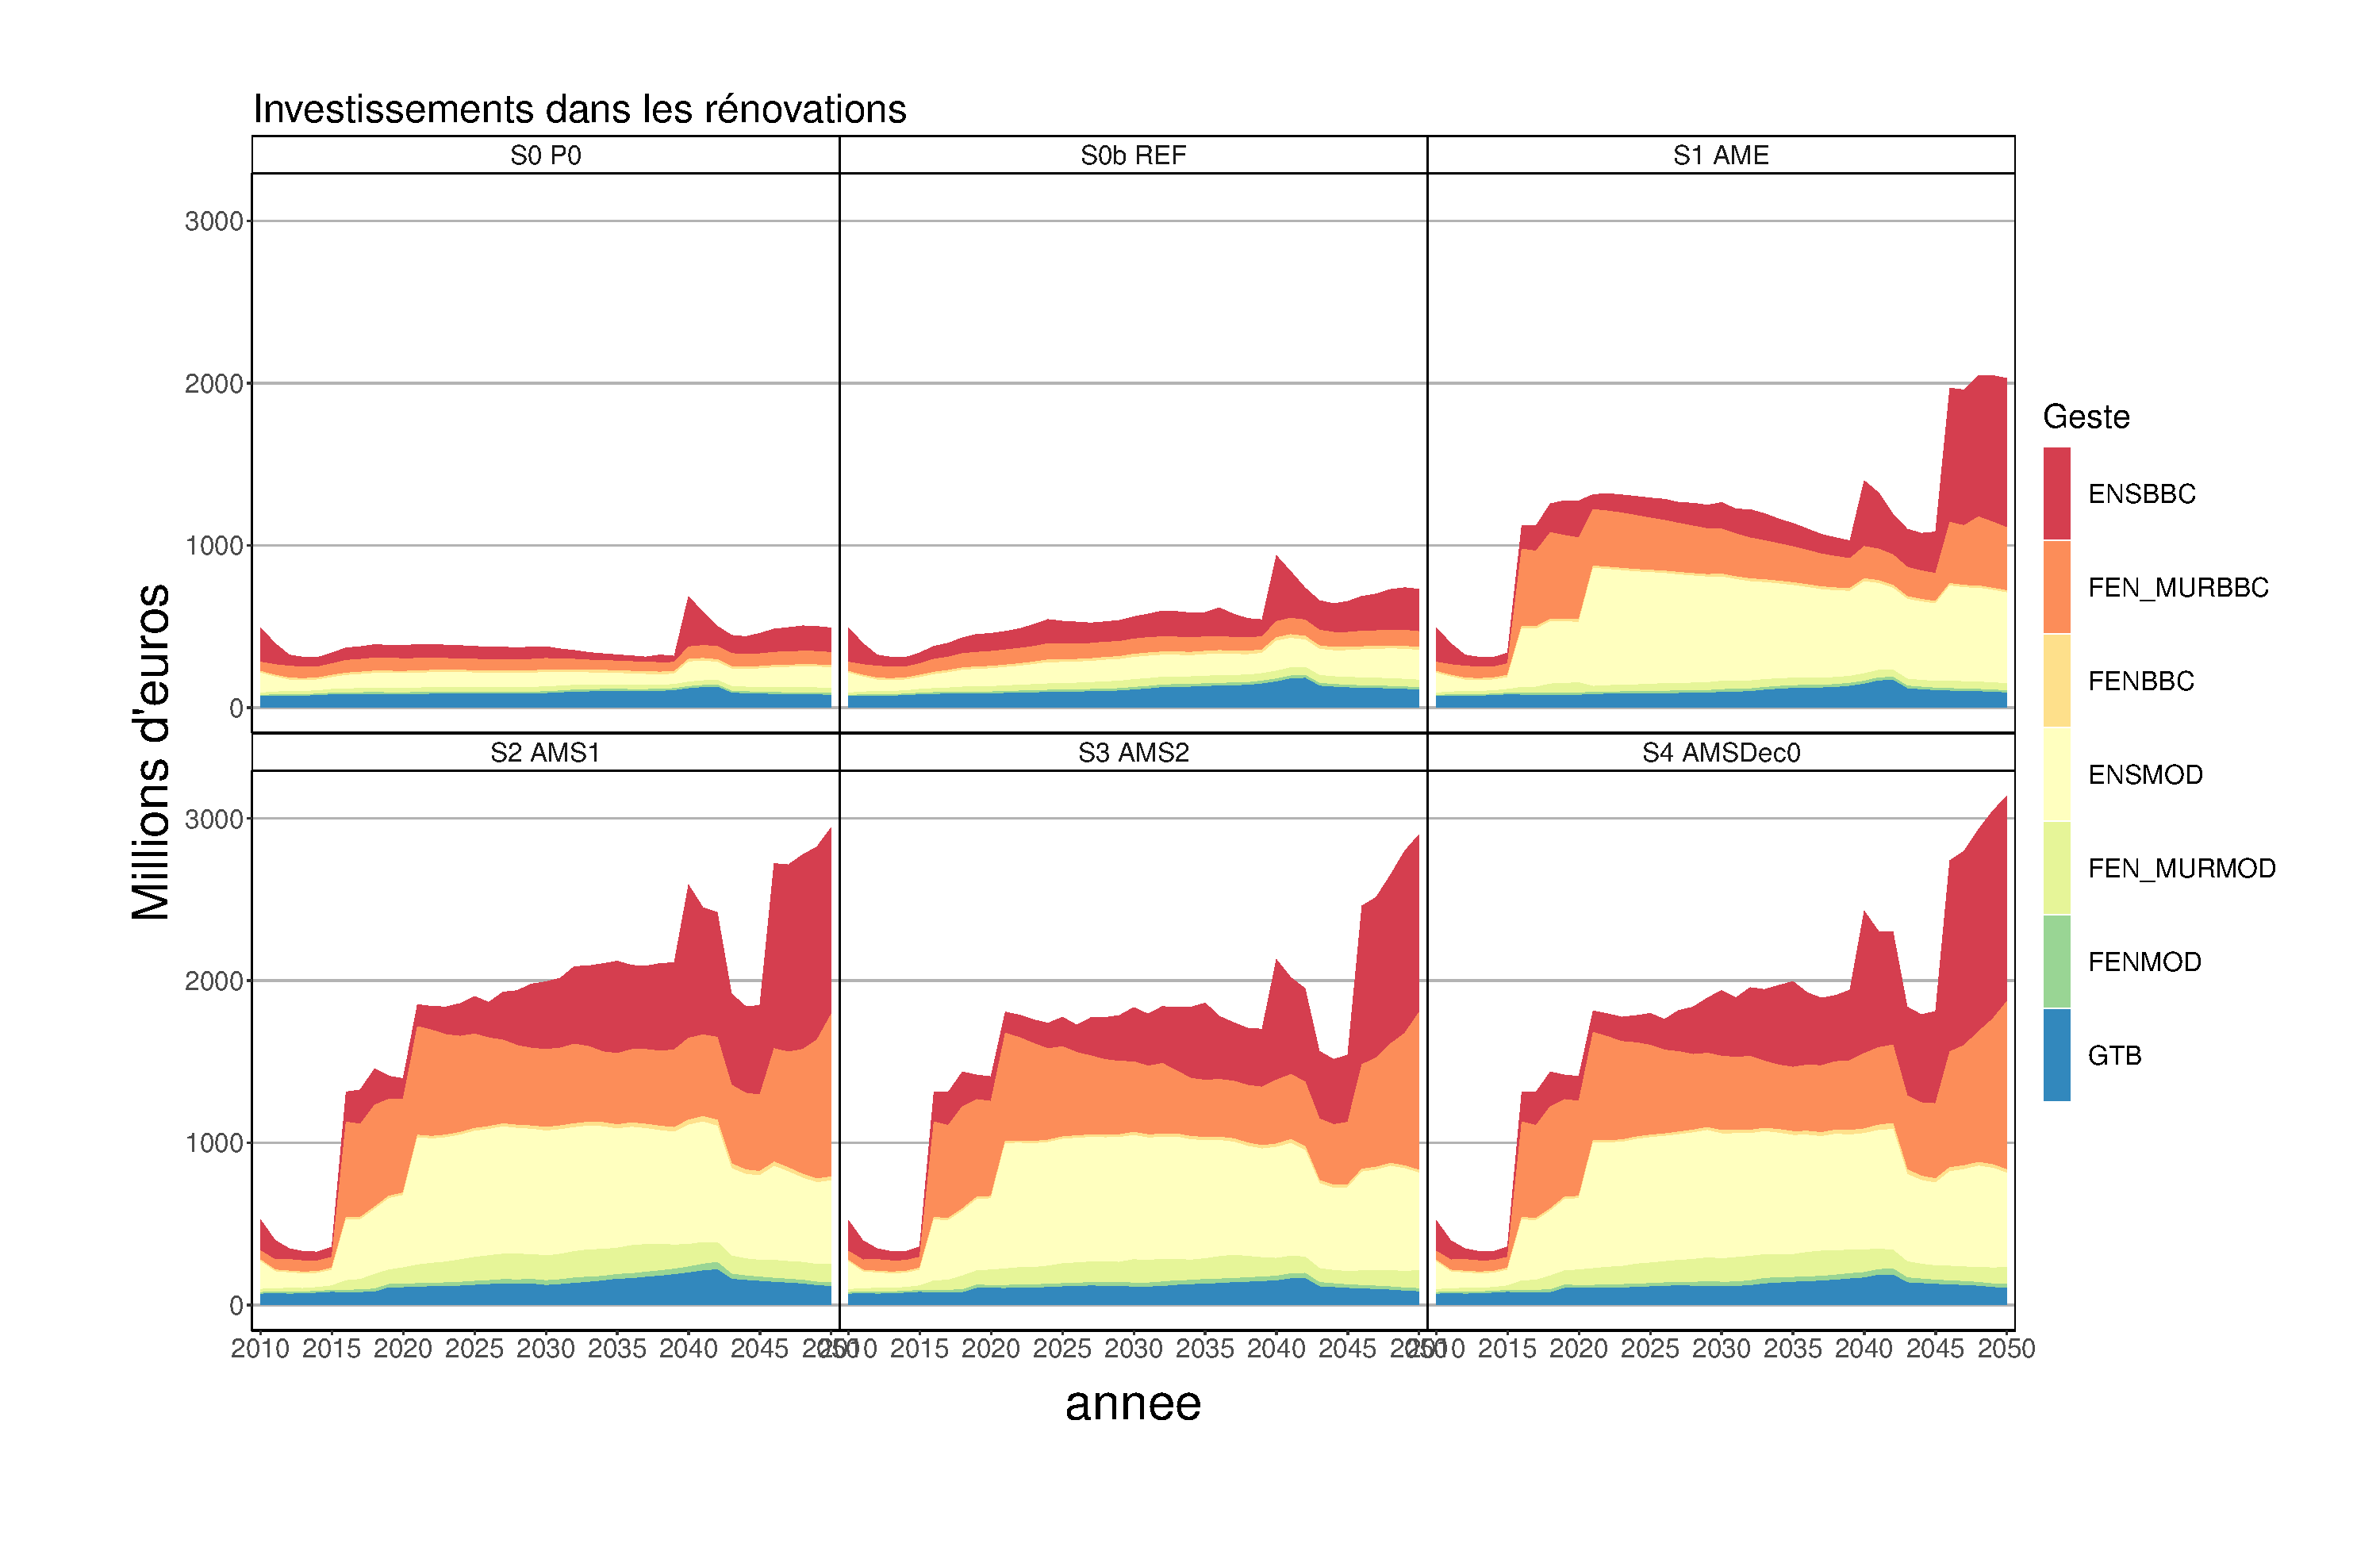
\includegraphics[width = 0.9\textwidth]{INV_Gestes-1}  
\end{figure}

Les gestes sur les fenêtres seules (\og~FENMOD~\fg et \og~FENBBC~\fg) sont peu réprésentés. En effet, en dehors des obligations de rénovation, le modèle sélectionne les gestes les plus rentables (coût global plus faible) chaque année et les gestes sur les fenêtres présentent des gains faibles pour des coûts importants au m². Ils sont donc peu sélectionnés contrairement à ce que l'on observe sur le marché des rénovations. Le décalage entre les simulations et lo'bserbvation peu s'expliquer par le fait que le choix de changer des fenêtres ne prend souvent pas seulement en compte l'efficacité énergétique mais aussi le confort ainsi que des considérations esthétiques. 


\begin{figure}[h!]
\centering 
\caption{Investissements dans les changements de systèmes}\label{INV_syst-1}  
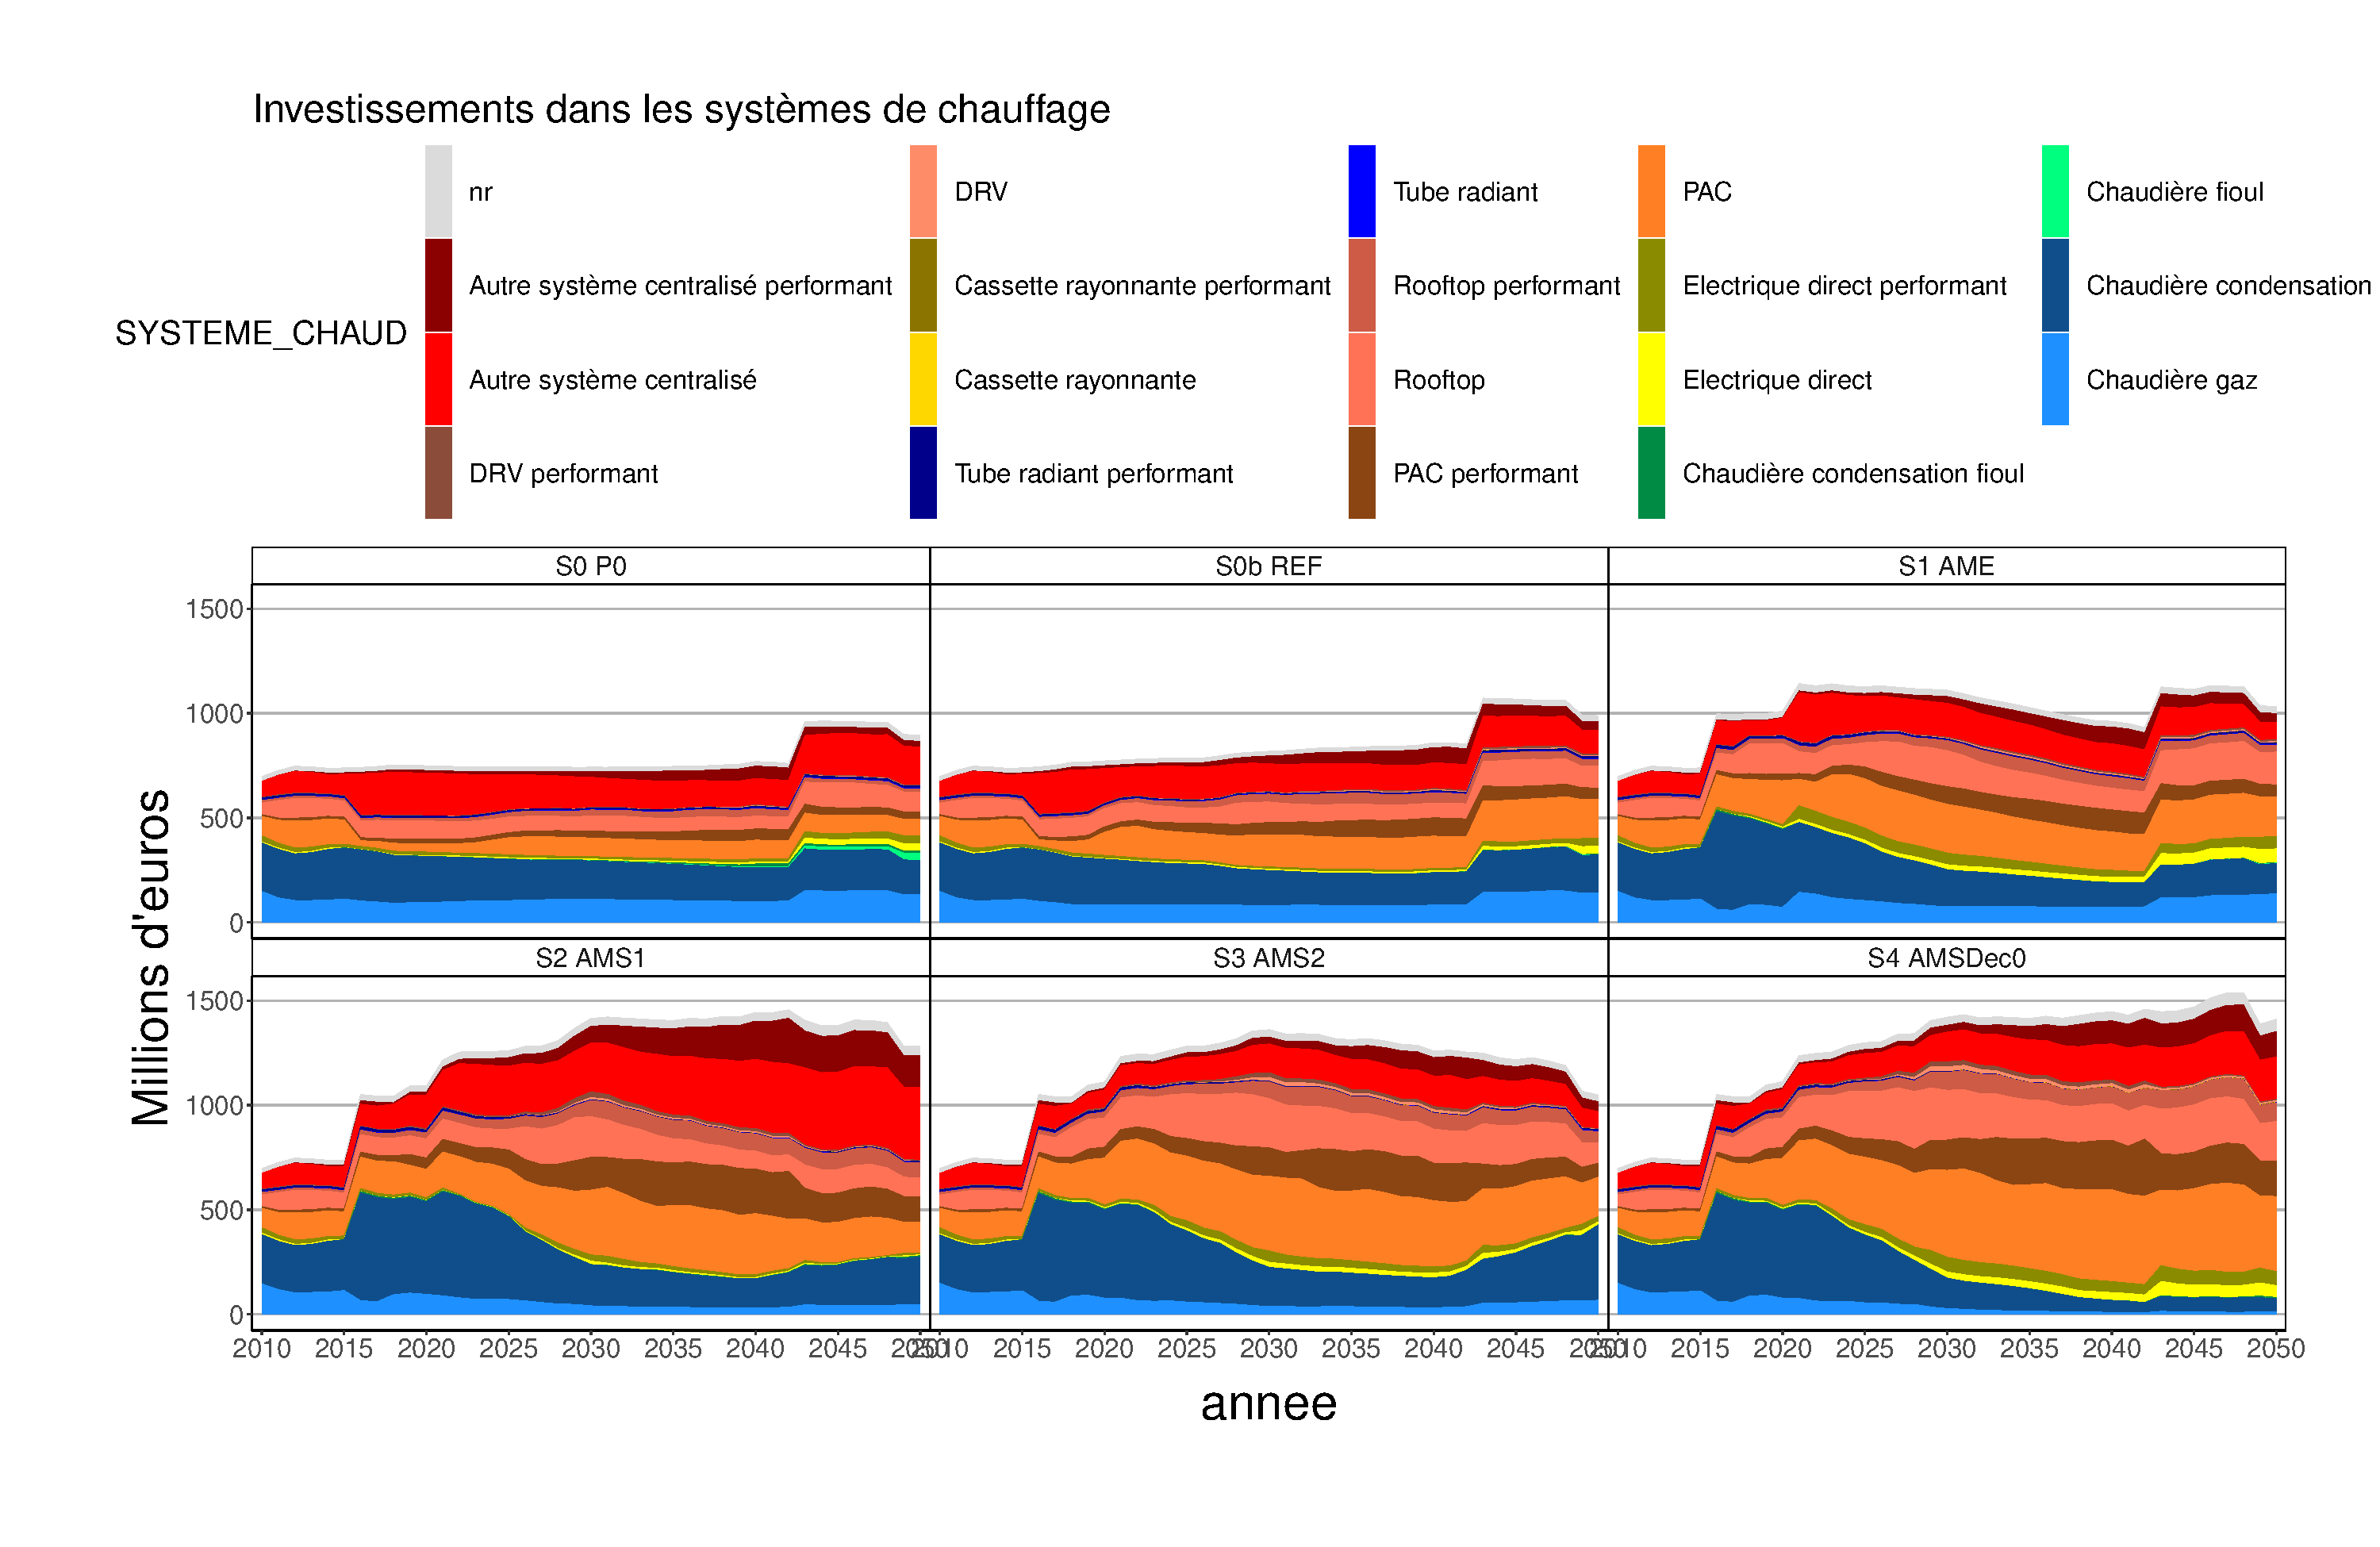
\includegraphics[width = 0.9\textwidth]{INV_syst-1}  
\end{figure}

En plus des investissements cumulés entre 2015 et 2050, le tableau \ref{Cumul_INV} montre aussi que les investissements couverts par des prêts bonifiés et par des CEE représentent 35~\% des investissements. 


\begin{table}[h] \caption{Investissements cumulés entre 2015 et 2050 et Investissements couverts par des prêts bonifiés et des CEE}\label{Cumul_INV}
\centering
\scriptsize
\begin{tabular}[c]{|l|c|c|c|c|c|c|}
\hline
				& Investissements cumulés & Dont prêts bonifiés & Dont CEE 	\\
\hline
P0 			&	43	&					0	 &										0	\\
REF 		&	51 	&					0  &										0 \\			
AME 		&	78 	&					0  &										1 \\					
AMS1 		&	107 &					19 &										19	\\				
AMS2 		&	98 	&					17 &			  						18 \\		
AMSDec0 &	106 & 				19 &										19	\\	
\hline
\end{tabular}
\end{table}

\clearpage

\subsection{Impacts économiques et efficience}

Dans cette partie, nous comparons les impacts économiques des différents scénarios simulés sur les usagers des bâtiments tertiaires, sur le budget de l’État et nous réalisons une analyse socio-économique des scénarios. Nous nous concentrons ici sur l'évolution des consommations de chauffage uniquement car c'est le seul usage pour lequel les investissements supplémentaires induits par les mesures simulées sont calculées par le modèle. Pour les autres usages, les économies d'énergie additionnelles apportées par les mesures simulées ne sont pas toujours associées à des surcoûts d'investissements ou seulement de manière partielle. 

D'autre part, nous réalisons le bilan économique uniquement sur le parc existant en 2015 car les investissements liées à la construction des bâtiments neufs ne sont pas comptabilisées dans le modèle. Enfin, bien que la dernière année simulée dans le modèle est 2050, les investissements réalisés en fin de période ont des bénéfices qui perdurent au delà de 2050. Nous considérons donc que les économies d'énergies, les réductions d'émissions de CO$_2$ et les recettes des taxes énergétiques restent à leur niveau de 2050 pendant 10 ans jusque 2060 tandis que les investissements sont considérés nuls après 2050. 

\subsubsection{Bilan pour l’État}

Le tableau \ref{Bilan_Etat} présente dans un premier temps le bilan des scénarios en ce qui concerne les recettes fiscales des taxes sur les énergies, la composante carbone et les subventions éventuelles liées à la décarbonation du mix énergétique (AMS2).  Le scénario AME présente un bilan positif de 5,2 Milliards d'euros pour l’État en comparaison avec le scénario sans mesures AME (REF) car même si les recettes des taxes énergétiques diminuent avec la baisse des consommations énergétiques du fait des mesures AME, elles sont compensées par la hausse des recettes de la composante carbone. 

Le scénario AMS1 présente un bilan fortement positif de 7,2 milliards d'euros par rapport au scénario AME car les usagers à la fois sont plus taxés à travers la hausse de la composante carbone (+ 4,1 milliards d'euros) mais aussi moins subventionnés car ils supportent le coût complet des énergies y compris la majoration de la CSPE sur l'électricité comptabilisée comme une subvention dans le scénario AME. Au contraire le scénario AMS2 résulte en une perte de 21,4 millards d'euros par rapport au scénario AME car la décarbonation des vecteurs énergétiques (électricité, biogaz, chauffage urbain) est entièrement couverte par des subventions de l’État. La hausse de la composante carbone par rapport au scénario AME permet néanmoins de rééquilibrer le bilan pour l’État mais il reste négatif (- 3,1 milliards d'euros). Enfin, dans le scénario AMSDec0 sans décarbonation, les recettes de la composante carbone augmentent fortement (+7 milliards d'euros par rapport aux scénarios AMS1 et AMS2) étant donné que le gaz n'est pas décarboné. Les recettes de la composante carbone restent notamment élevées y compris après 2050 contrairement aux deux scénarios précédents (cf figure \ref{Evol_Recettes_taxes-1}). 



\begin{table}[h] \caption{Bilan des scénarios pour le budget de l’État entre 2015 et 2060}\label{Bilan_Etat}
\begin{center}
\begin{tabular}[c]{|l|c|c|c|c|c|c|}
\hline
								&Recettes CC & Subventions  &Autres recettes fiscales & Total \\
								& 					 & prêts bonifiés & (taxes - subventions) & \\
								&		(G\euro) &			(G\euro) 	& (G\euro) 					& (G\euro)	 \\			
\hline
P0 	&9.6 & 0 &4.4 &13.9 \\
REF & 9.0 & 0 &3.9 &12.9 \\
AME &15.1 & 0&3.0 &18.1 \\
AMS1 &19.2 &1.2 &7.3 &25.3 \\
AMS2 &19.3 & 1.1&-21.3 &-3.1 \\
AMSDec0 &26.5 & 1.1 &3.9 &29.3 \\
\hline
\end{tabular}
\end{center}

\footnotesize{Note de lecture : Les grandeurs sont cumulées entre 2015 et 2060 et actualisées au taux public de 4,5~\%.  Les autres recettes fiscales incluent les taxes sur les énergies (hors composante carbone), les subventions éventuelles liées à la décarbonation du mix énergétique (Scénarios AMS2) et la composante énergie entre 2040 et 2050 (scénarios AMS1 et AMSDec0). On considère que les recettes des taxes et les subventions sur le prix des énergies pour l'année 2050 sont prolongées pendant 10 ans jusque 2060. Les subventions correspondant aux prêts bonifiés sont calculées comme la différence entre les annuités payées sur 10 ans pour un prêt bancaire classique avec un taux d'intérêt de 3~\% et celles payées sur 10 ans pour un prêts bonifiés avec un taux d'intérêt de 1~\%.}
\end{table}

% \begin{longtable}[]{@{}crrr@{}}
\caption{bilan pour l'Etat}\tabularnewline
\toprule
\begin{minipage}[b]{0.21\columnwidth}\centering\strut
~\strut
\end{minipage} & \begin{minipage}[b]{0.17\columnwidth}\raggedleft\strut
Recettes CC\strut
\end{minipage} & \begin{minipage}[b]{0.30\columnwidth}\raggedleft\strut
Recettes autres taxes\strut
\end{minipage} & \begin{minipage}[b]{0.09\columnwidth}\raggedleft\strut
Total\strut
\end{minipage}\tabularnewline
\midrule
\endfirsthead
\toprule
\begin{minipage}[b]{0.21\columnwidth}\centering\strut
~\strut
\end{minipage} & \begin{minipage}[b]{0.17\columnwidth}\raggedleft\strut
Recettes CC\strut
\end{minipage} & \begin{minipage}[b]{0.30\columnwidth}\raggedleft\strut
Recettes autres taxes\strut
\end{minipage} & \begin{minipage}[b]{0.09\columnwidth}\raggedleft\strut
Total\strut
\end{minipage}\tabularnewline
\midrule
\endhead
\begin{minipage}[t]{0.21\columnwidth}\centering\strut
\textbf{S0 P0}\strut
\end{minipage} & \begin{minipage}[t]{0.17\columnwidth}\raggedleft\strut
9.7\strut
\end{minipage} & \begin{minipage}[t]{0.30\columnwidth}\raggedleft\strut
7.0\strut
\end{minipage} & \begin{minipage}[t]{0.09\columnwidth}\raggedleft\strut
16.7\strut
\end{minipage}\tabularnewline
\begin{minipage}[t]{0.21\columnwidth}\centering\strut
\textbf{S0b REF}\strut
\end{minipage} & \begin{minipage}[t]{0.17\columnwidth}\raggedleft\strut
9.1\strut
\end{minipage} & \begin{minipage}[t]{0.30\columnwidth}\raggedleft\strut
6.5\strut
\end{minipage} & \begin{minipage}[t]{0.09\columnwidth}\raggedleft\strut
15.7\strut
\end{minipage}\tabularnewline
\begin{minipage}[t]{0.21\columnwidth}\centering\strut
\textbf{S1 AME}\strut
\end{minipage} & \begin{minipage}[t]{0.17\columnwidth}\raggedleft\strut
15.2\strut
\end{minipage} & \begin{minipage}[t]{0.30\columnwidth}\raggedleft\strut
5.7\strut
\end{minipage} & \begin{minipage}[t]{0.09\columnwidth}\raggedleft\strut
20.9\strut
\end{minipage}\tabularnewline
\begin{minipage}[t]{0.21\columnwidth}\centering\strut
\textbf{S2 AMS1}\strut
\end{minipage} & \begin{minipage}[t]{0.17\columnwidth}\raggedleft\strut
19.3\strut
\end{minipage} & \begin{minipage}[t]{0.30\columnwidth}\raggedleft\strut
10.1\strut
\end{minipage} & \begin{minipage}[t]{0.09\columnwidth}\raggedleft\strut
29.4\strut
\end{minipage}\tabularnewline
\begin{minipage}[t]{0.21\columnwidth}\centering\strut
\textbf{S3 AMS2}\strut
\end{minipage} & \begin{minipage}[t]{0.17\columnwidth}\raggedleft\strut
19.4\strut
\end{minipage} & \begin{minipage}[t]{0.30\columnwidth}\raggedleft\strut
-13.7\strut
\end{minipage} & \begin{minipage}[t]{0.09\columnwidth}\raggedleft\strut
5.7\strut
\end{minipage}\tabularnewline
\begin{minipage}[t]{0.21\columnwidth}\centering\strut
\textbf{S4 AMSDec0}\strut
\end{minipage} & \begin{minipage}[t]{0.17\columnwidth}\raggedleft\strut
26.6\strut
\end{minipage} & \begin{minipage}[t]{0.30\columnwidth}\raggedleft\strut
11.8\strut
\end{minipage} & \begin{minipage}[t]{0.09\columnwidth}\raggedleft\strut
38.4\strut
\end{minipage}\tabularnewline
\bottomrule
\end{longtable}

\begin{figure}[h!]
\centering 
\caption{Recettes fiscales de l'ensemble des taxes et subventions sur les énergies (CC comprise) par scénario }\label{Evol_Recettes_taxes-1}  
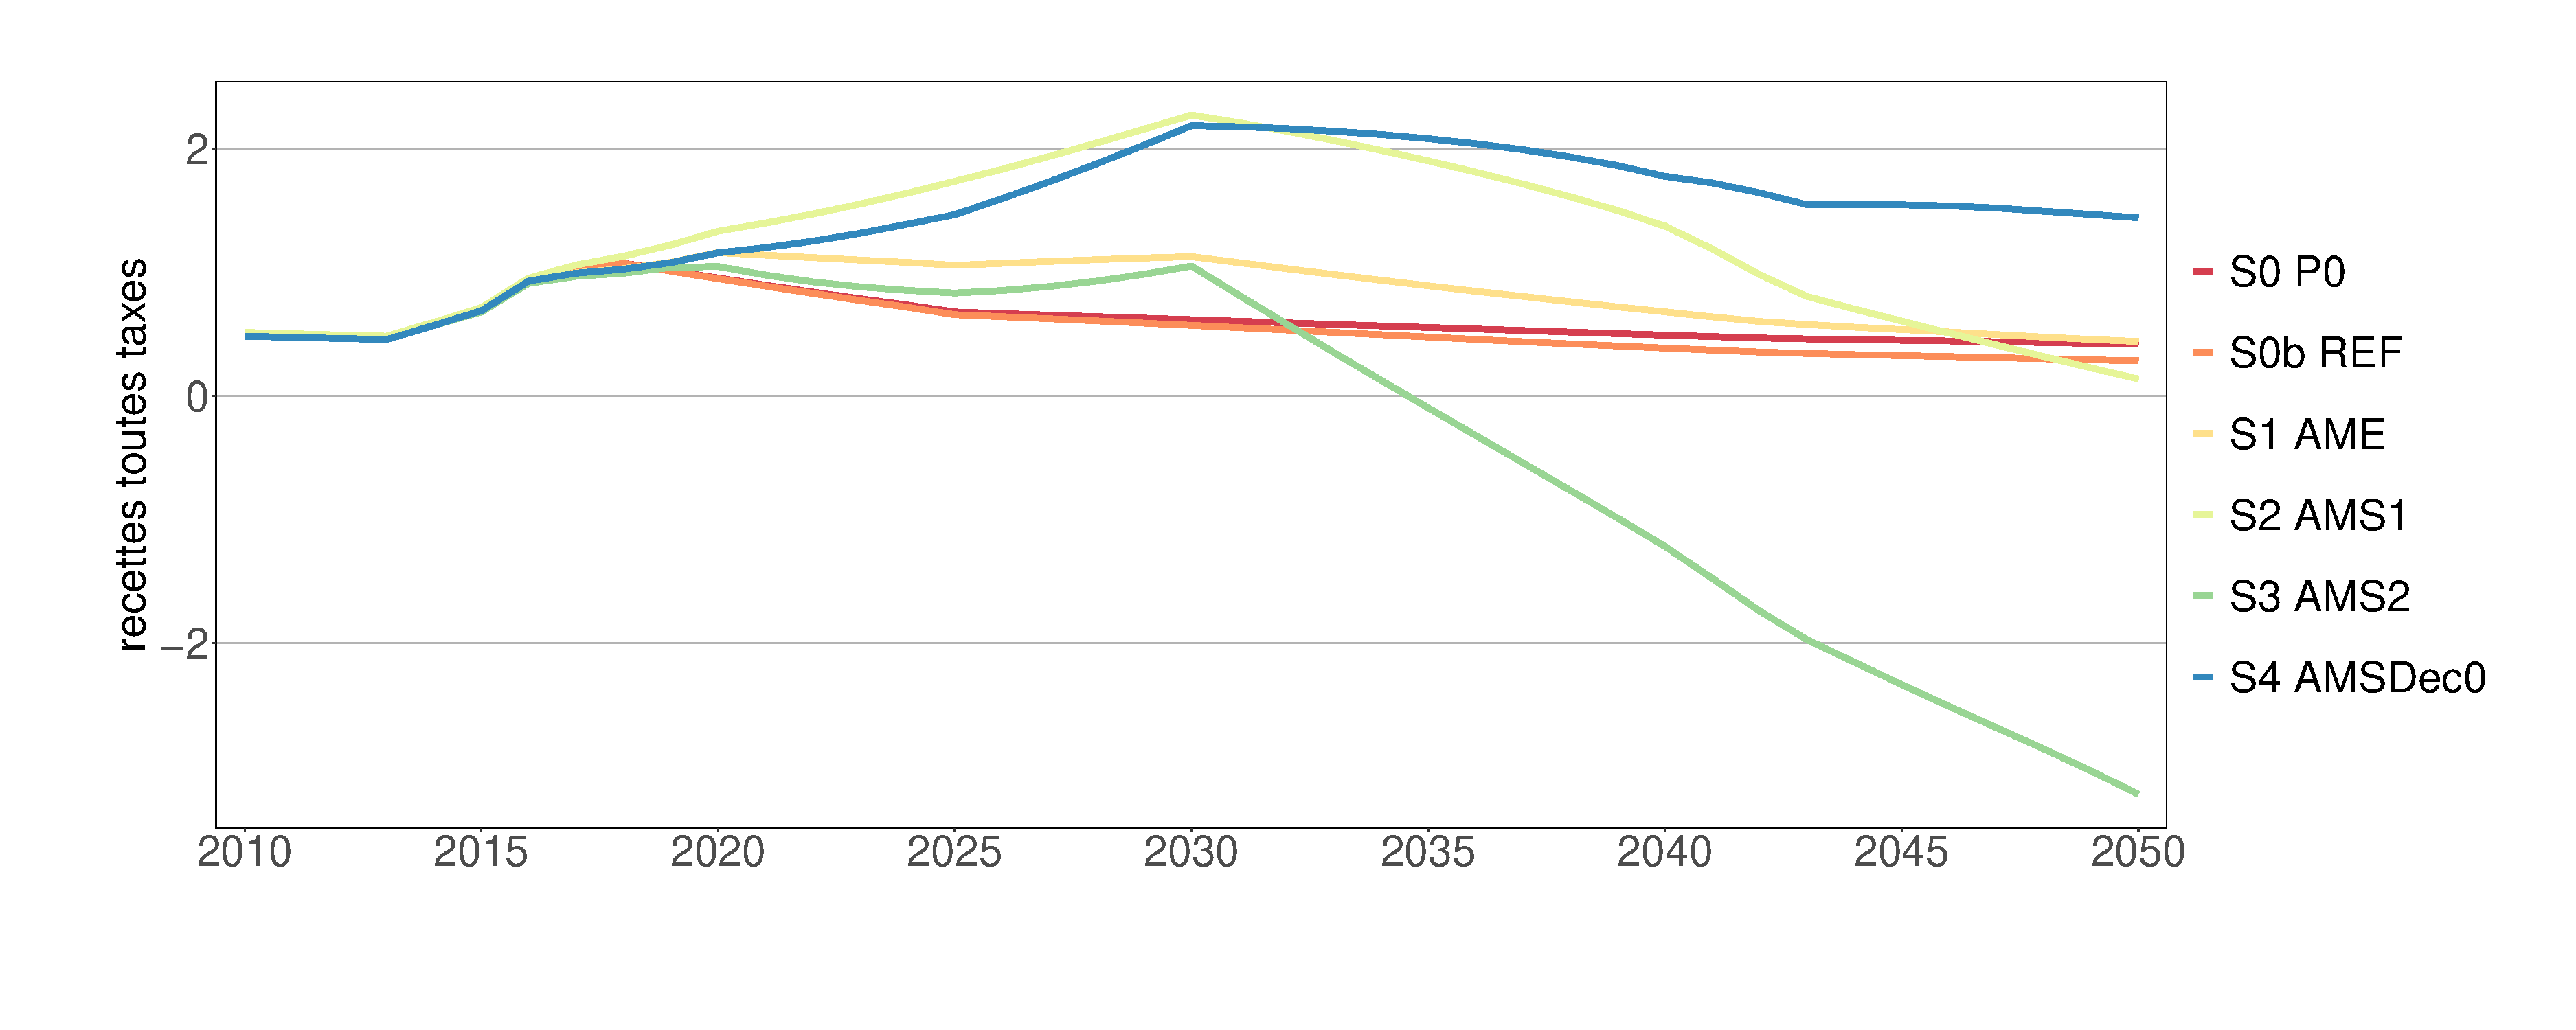
\includegraphics[width = 0.9\textwidth]{Evol_Recettes_taxes-1}  
\end{figure}

\clearpage 

\subsubsection{Bilan pour les usagers}
%
\begin{longtable}[]{@{}crrrrrrr@{}}
\caption{bilan pour les usagers}\tabularnewline
\toprule
\begin{minipage}[b]{0.10\columnwidth}\centering\strut
~\strut
\end{minipage} & \begin{minipage}[b]{0.11\columnwidth}\raggedleft\strut
Investissements\strut
\end{minipage} & \begin{minipage}[b]{0.06\columnwidth}\raggedleft\strut
Facture\strut
\end{minipage} & \begin{minipage}[b]{0.13\columnwidth}\raggedleft\strut
Facture (Conso AME)\strut
\end{minipage} & \begin{minipage}[b]{0.07\columnwidth}\raggedleft\strut
Emissions\strut
\end{minipage} & \begin{minipage}[b]{0.09\columnwidth}\raggedleft\strut
Consommations\strut
\end{minipage} & \begin{minipage}[b]{0.08\columnwidth}\raggedleft\strut
Coût total\strut
\end{minipage} & \begin{minipage}[b]{0.14\columnwidth}\raggedleft\strut
Coût total (Conso AME)\strut
\end{minipage}\tabularnewline
\midrule
\endfirsthead
\toprule
\begin{minipage}[b]{0.10\columnwidth}\centering\strut
~\strut
\end{minipage} & \begin{minipage}[b]{0.11\columnwidth}\raggedleft\strut
Investissements\strut
\end{minipage} & \begin{minipage}[b]{0.06\columnwidth}\raggedleft\strut
Facture\strut
\end{minipage} & \begin{minipage}[b]{0.13\columnwidth}\raggedleft\strut
Facture (Conso AME)\strut
\end{minipage} & \begin{minipage}[b]{0.07\columnwidth}\raggedleft\strut
Emissions\strut
\end{minipage} & \begin{minipage}[b]{0.09\columnwidth}\raggedleft\strut
Consommations\strut
\end{minipage} & \begin{minipage}[b]{0.08\columnwidth}\raggedleft\strut
Coût total\strut
\end{minipage} & \begin{minipage}[b]{0.14\columnwidth}\raggedleft\strut
Coût total (Conso AME)\strut
\end{minipage}\tabularnewline
\midrule
\endhead
\begin{minipage}[t]{0.10\columnwidth}\centering\strut
\textbf{S0 P0}\strut
\end{minipage} & \begin{minipage}[t]{0.11\columnwidth}\raggedleft\strut
28\strut
\end{minipage} & \begin{minipage}[t]{0.06\columnwidth}\raggedleft\strut
155\strut
\end{minipage} & \begin{minipage}[t]{0.13\columnwidth}\raggedleft\strut
143\strut
\end{minipage} & \begin{minipage}[t]{0.07\columnwidth}\raggedleft\strut
662\strut
\end{minipage} & \begin{minipage}[t]{0.09\columnwidth}\raggedleft\strut
3,437\strut
\end{minipage} & \begin{minipage}[t]{0.08\columnwidth}\raggedleft\strut
183\strut
\end{minipage} & \begin{minipage}[t]{0.14\columnwidth}\raggedleft\strut
170\strut
\end{minipage}\tabularnewline
\begin{minipage}[t]{0.10\columnwidth}\centering\strut
\textbf{S0b REF}\strut
\end{minipage} & \begin{minipage}[t]{0.11\columnwidth}\raggedleft\strut
31\strut
\end{minipage} & \begin{minipage}[t]{0.06\columnwidth}\raggedleft\strut
170\strut
\end{minipage} & \begin{minipage}[t]{0.13\columnwidth}\raggedleft\strut
159\strut
\end{minipage} & \begin{minipage}[t]{0.07\columnwidth}\raggedleft\strut
619\strut
\end{minipage} & \begin{minipage}[t]{0.09\columnwidth}\raggedleft\strut
3,210\strut
\end{minipage} & \begin{minipage}[t]{0.08\columnwidth}\raggedleft\strut
201\strut
\end{minipage} & \begin{minipage}[t]{0.14\columnwidth}\raggedleft\strut
190\strut
\end{minipage}\tabularnewline
\begin{minipage}[t]{0.10\columnwidth}\centering\strut
\textbf{S1 AME}\strut
\end{minipage} & \begin{minipage}[t]{0.11\columnwidth}\raggedleft\strut
44\strut
\end{minipage} & \begin{minipage}[t]{0.06\columnwidth}\raggedleft\strut
166\strut
\end{minipage} & \begin{minipage}[t]{0.13\columnwidth}\raggedleft\strut
166\strut
\end{minipage} & \begin{minipage}[t]{0.07\columnwidth}\raggedleft\strut
545\strut
\end{minipage} & \begin{minipage}[t]{0.09\columnwidth}\raggedleft\strut
2,818\strut
\end{minipage} & \begin{minipage}[t]{0.08\columnwidth}\raggedleft\strut
210\strut
\end{minipage} & \begin{minipage}[t]{0.14\columnwidth}\raggedleft\strut
210\strut
\end{minipage}\tabularnewline
\begin{minipage}[t]{0.10\columnwidth}\centering\strut
\textbf{S2 AMS1}\strut
\end{minipage} & \begin{minipage}[t]{0.11\columnwidth}\raggedleft\strut
56\strut
\end{minipage} & \begin{minipage}[t]{0.06\columnwidth}\raggedleft\strut
182\strut
\end{minipage} & \begin{minipage}[t]{0.13\columnwidth}\raggedleft\strut
196\strut
\end{minipage} & \begin{minipage}[t]{0.07\columnwidth}\raggedleft\strut
353\strut
\end{minipage} & \begin{minipage}[t]{0.09\columnwidth}\raggedleft\strut
2,564\strut
\end{minipage} & \begin{minipage}[t]{0.08\columnwidth}\raggedleft\strut
238\strut
\end{minipage} & \begin{minipage}[t]{0.14\columnwidth}\raggedleft\strut
252\strut
\end{minipage}\tabularnewline
\begin{minipage}[t]{0.10\columnwidth}\centering\strut
\textbf{S3 AMS2}\strut
\end{minipage} & \begin{minipage}[t]{0.11\columnwidth}\raggedleft\strut
53\strut
\end{minipage} & \begin{minipage}[t]{0.06\columnwidth}\raggedleft\strut
169\strut
\end{minipage} & \begin{minipage}[t]{0.13\columnwidth}\raggedleft\strut
175\strut
\end{minipage} & \begin{minipage}[t]{0.07\columnwidth}\raggedleft\strut
356\strut
\end{minipage} & \begin{minipage}[t]{0.09\columnwidth}\raggedleft\strut
2,580\strut
\end{minipage} & \begin{minipage}[t]{0.08\columnwidth}\raggedleft\strut
222\strut
\end{minipage} & \begin{minipage}[t]{0.14\columnwidth}\raggedleft\strut
227\strut
\end{minipage}\tabularnewline
\begin{minipage}[t]{0.10\columnwidth}\centering\strut
\textbf{S4 AMSDec0}\strut
\end{minipage} & \begin{minipage}[t]{0.11\columnwidth}\raggedleft\strut
55\strut
\end{minipage} & \begin{minipage}[t]{0.06\columnwidth}\raggedleft\strut
175\strut
\end{minipage} & \begin{minipage}[t]{0.13\columnwidth}\raggedleft\strut
190\strut
\end{minipage} & \begin{minipage}[t]{0.07\columnwidth}\raggedleft\strut
477\strut
\end{minipage} & \begin{minipage}[t]{0.09\columnwidth}\raggedleft\strut
2,472\strut
\end{minipage} & \begin{minipage}[t]{0.08\columnwidth}\raggedleft\strut
230\strut
\end{minipage} & \begin{minipage}[t]{0.14\columnwidth}\raggedleft\strut
246\strut
\end{minipage}\tabularnewline
\bottomrule
\end{longtable}
Le tableau \ref{Bilan_usager} présente l'impact des différents scénarios pour les usagers/gestionnaires des bâtiments. Les mesures des scénarios AME et AMS entraînent des investissements supplémentaires pour les usagers qui diminuent leurs consommations de chauffage (cumulées sur la période). L'impact sur la facture énergétique dépend cependant du niveau des prix des énergies (taxes comprises). 

Le scénario AME permet aux usagers de réduire leur facture énergétique de 4 milliards d'euros pour des investissements supplémentaires de 13 milliards d'euros. Les mesures AME entraînent donc un surcoût de 9 milliards d'euros pour les usagers par rapport au scénario REF sans ces mesures.

La facture cumulée pour les scénario AMS est supérieure à celle du scénario AME malgré des baisses importantes des consommations de chauffage.  Par rapport au scénario AME, les 3 scénarios AMS entraînent des coûts supplémentaires pour les usagers entre 12 milliards d'euros dans le scénario AMS2 où les prix des énergies restent faibles et 28 milliards d'euros dans le scénario AMS1 où les prix sont très élevés car ils incluent le coût complet de décarbonation des énergies.  Le scénario AMSDec0 est celui qui permet de réduire le plus les consommations des usagers mais pas leur facture énergétique du fait du fort poids de la composante carbone. 

\begin{table}[h] \caption{Coût total par scénario entre 2015 et 2060 pour les usagers des bâtiments}\label{Bilan_usager}
\begin{center}
\scriptsize
\begin{tabular}[c]{|l|c|c|c|c|c|c|}
\hline
					& Investissements &  Consommations 		&	Facture  		 & Coût total & Facture 		& Coût total  \\
					&									& 	de chauffage		& énergétique & 	 usager		& (Conso AME)	&	(Conso AME) \\
					&		(G\euro)		&			(TWh)				&		(G\euro) 					& (G\euro)	 	& (G\euro) 					& (G\euro) \\
					&    (1) 				&      (2)        &      (3)            & (1)+(3) = (4) &  (5) & (1)+(5) = (6) \\
\hline
P0 				&			21				&			1~668 			&			114   					&			135  		&		  						&		\\
REF 			&			25 				&			1~601 			&			128   					&			153  		&		  						&	 \\
AME 			&			38 				&			1~436 			&			124   					&			162  		&		124  						&	162 \\
AMS1 			&			50 				&			1~359 			&			140   					&			190  		&		154  						& 204 \\
AMS2 			&			46 				&			1~362 			&			127		 					&			174  		&		133  						&	180 \\
AMSDec0 	&			49 				&			1~336 			&			134   					&			183  		&		149  						&	198 \\
\hline
\end{tabular}
\end{center}
\footnotesize{Note de lecture : Les grandeurs sont cumulées entre 2015 et 2060 et actualisées au taux public de 4,5~\%.  La facture énergétique est calculée en multipliant les consommations aux prix des énergies HTVA mais incluant l'ensemble des taxes sur les énergies (y compris la composante carbone et la composante énergie)  On considère que les consommations pour l'année 2050 sont prolongées pendant 10 ans jusque 2060. Les investissements incluent la partie financées par les CEE}
\end{table}


Les coûts totaux pour les usagers doivent néanmoins être comparés à ceux qu'ils auraient subi s'ils n'avaient pas investi dans la rénovation énergétique de leurs bâtiments c'est à dire si leurs consommations étaient restées au niveau de celle du scénario AME et si les prix des énergies avaient augmenté fortement comme dans les scénarios AMS ( colonnes (5) et (6) du tableau \ref{Bilan_usager}). Ainsi pour le scénario AMS1, le surcoût par rapport au scénario AME serait de 42 milliards d'euros sans investir contre 28 milliards d'euros avec des investissements de 12 milliards d'euros dans la rénovation. Il est donc rentable d'investir pour les usagers. Pour le scénario AMSDecO sans décarbonation, le surcoût par rapport au scénario AME serait de 36 milliards d'euros sans investir contre 21 milliards d'euros avec des investissements de 11 milliards d'euros dans la rénovation. Pour ces deux scénarios, les investissements dans la rénovation sont rentables pour les usagers. 

Pour le scénario AMS2, le surcoût par rapport au scénario AME serait de 18 milliards d'euros sans investir contre 12 milliards d'euros avec des investissements de 8 milliards d'euros dans la rénovation. Les investissements sont peu rentables du fait des prix bas dans ce scénario (décarbonation subventionnée)

D'autre part, les surcoûts pour les usagers par rapport au scénario AME sont à comparer aux recettes additionnelles générées par les taxes sur les énergies qui peuvent leur être redistribuées (tableau \ref{Bilan_Etat}). Ainsi les 7,2 milliards d'euros de recettes supplémentaires pour le scénario AMS1, et 11,2 milliards d'euros pour le scénario AMSDec0 permettraient de compenser respectivement 26~\% et 53~\% des surcoûts payées par les usagers.


\newpage 
\clearpage 


\cadrevert{Coûts d’abattement $CO_2$ et analyse socio-économique}{
\vspace{0.2cm}
{\fontsize{7}{8}\selectfont

Dans le calcul socio-économique classique, le principe général d’un coût d’abattement consiste (i) à évaluer le surcoût associé à l'activation d'un levier technologique ou comportemental, par rapport à un scénario de référence (non ou moindre activation de ce levier) ; (ii) à lui retrancher d'éventuels bénéfices (en général une économie d’énergie, mais éventuellement d’autres bénéfices tels qu'une diminution de la pollution atmosphérique, de nuisances sonores, de la congestion, etc.) ; (iii) à rapporter cette différence aux émissions de GES évitées et actualisées. Ceci est résumé par la formule générale :

$C_{CO_2} = \frac{\textrm{Investissement} - \textrm{GainEnergie} - \textrm{GainAutresExternalités}}{\textrm{EmissionsEvitées}} $

En toute logique, le calcul du coût d'abattement suit donc les principes de l'analyse socio-économique : 
\begin{itemize}
	\item les investissements et gains éventuels sont évalués sur la base de \text{coûts hors taxes} : en particulier, on travaille hors TVA et hors TICPE, TICFE, etc. pour les dépenses énergétiques ;
	\item les gains associés aux émissions évitées et autres externalités sont calculés en tenant compte du mieux possible des phases de production amont et aval (approche cycle de vie) ; 
	\item il faut théoriquement prendre également en compte le \text{COFP} (coût d’opportunité des fonds public) dans les coûts au numérateur ;
	\item l’ensemble des grandeurs sont \text{actualisées} au taux public de 4,5~\% \citep{Quinet2013}. 
\end{itemize}

Selon que l'on actualise ou non les émissions évitées, le coût d'abattement calculé s’interprète de manière différente :

Si on actualise les émissions, le coût d’abattement socio-économique  s’interpréter comme la valeur du carbone, constante (en euros constants) sur la durée de vie de l’investissement, permettant de rentabiliser celui-ci du point de vue de la collectivité, c'est-à-dire d’annuler sa valeur (socio-économique) actuelle nette. Si on n'actualise pas les émissions évitées, il s’interprète comme la valeur initiale du carbone qui doit croître au taux d'actualisation public pour rentabiliser les investissements. 
Il vérifie l’équation suivante d’annulation de la VAN  :

$VAN = \sum_t(\textrm{Investissement}_t - \textrm{GainEnergie}_t - \textrm{GainAutresExternalités}_t - C_{CO_2}^t*\textrm{EmissionsEvitées}_t = 0$

où $C_{CO_2}^t = C_{CO_2} = \textrm{cste}$ si on actualise les émissions évitées et $C_{CO_2}^t = (1+a)^t*C_{CO_2}$ sinon. 

Le coût d'abattement socio-économique ainsi calculé caractérise le levier (technologique ou comportemental) étudié et renseigne uniquement sur sa rentabilité potentielle du point de vue de la collectivité (dans la mesure où il suit les principes du calcul public et ne distingue pas les efforts des différentes catégories d'agents).

Appliquée à la comparaison de deux scénarios de rénovation énergétique des bâtiments tertiaire entre deux années 2015 et 2050 (scénarios SIM et REF), le calcul du coût d'abattement devient : 

$C_{CO_2} = \frac{
\sum_{t=2015}^{2050} \frac{\textrm{InvestissementSIM}_t -\textrm{InvestissementREF}_t  + \textrm{FactureEnergieHTSIM}_t - \textrm{FactureEnergieHTREF}_t + \textrm{COFPSIM}_t - \textrm{COFPREF}_t}{(1+a)^t}}{\sum_{t=2015}^{2050} \textrm{EmissionsREF}_t-\textrm{EmissionsSIM}_t} $ 

Les investissements utilisés sont l'ensemble des investissements dans la rénovation énergétique (rénovation du bâti et changements de système de chauffage). La facture énergétique est calcul en multipliant les consommations de chauffage des bâtiments par énergie du scénario aux prix des énergies hors TVA, hors composante carbone et hors les autres taxes sur les énergies (TICFE, TICPE, TICGN, composante énergie...).  Le COPFP est calculé en considérant qu'il représente 25~\% du montant des recettes des taxes sur les consommations d'énergie moins les subventions versées par l’État. Les émissions ne sont pas actualisées dans ce calcul. Toutes les autres grandeurs le sont.

Le coût d'abattement socio-économique ainsi calculé caractérise la rentabilité de l'ensemble des mesures supplémentaires simulées dans le scénario SIM par rapport au scénario de référence REF

}}
\newpage 

\subsubsection{Bilan socio-économique}

Le tableau \ref{Bilan_socio} présente le bilan des scénarios du point de vue de l'ensemble de la société : Les investissements cumulés et actualisés entre 2015 et 2050 (colonne (1)), la facture énergétique hors taxes et subventions cumulée et actualisée entre 215 et 2060 (colonne (2)), les émissions de CO$_2$ cumulées entre 2015 et 2060 (colonne (3)), le coût d'opportunité des fonds publics cumulés et actualisés entre 2015 et 2060 (colonne (6)). Les coûts d'abattements sont calculés comme décrit dans l'encadré \og~Coûts d’abattement $CO_2$ et analyse socio-économique~\fg en prenant comme scénario de référence le scénario AME. Par exemple, le surcoût pour le scénario AMS1 est égal à l'écart d'investissement par rapport au scénario AME ($50 - 38 = 12$ milliards d'euros) plus l'écart de facture énergétique par rapport au scénario AME ($114 - 106 = 8$ milliards d'euros) plus l'écart de COFP ($-6,3 - (-4,5) = -1,8$ milliards d'euros). Le coût de la tonne de CO$_2$ évitée (colonne (8)) est égal à ce surcoût ($12+11-2= 18$ G\euro)  rapporté aux émissions évitées par rapport au scénario AME ($520 - 332 = 188$ MtCO$_2$). La différence entre les coûts d'abattement des colonnes (5) et (6) provient du fait que celui de la colonne (5) n'inclut pas le COFP. Il permet d'estimer l'impact des recettes fiscales ou des dépenses budgétaires supplémentaires liés aux scénarios sur le coût à la tonne de CO$_2$ évitée. 

Les coûts d'abattement calculés pour les scénario P0 et REF correspondent en fait aux coûts d'abattement pour passer du scénario P0 (respectivement REF) au scénario AME. Par rapport au scénario REF, les mesures mises en place dans le scénario AME ont donc un coût à la tonne de CO$_2$ évitée faible autour de 32~\euro/tCO$_2$. Les mesures mises en place par les scénarios AMS ont un coût  à la tonne de CO$_2$ évitée plus élevé entre 84 et 206 ~\euro/tCO$_2$. En effet, plus les réductions d'émissions sont importantes, plus les gisements de réduction des émissions restants sont coûteux. 

Sur le plan de la facture énergétique pour l'ensemble de la société (colonne (2)), le scénario AMS2 est le plus coûteux (15 milliards d'euros de plus que le scénario AMS1). En effet, les prix des énergies sont bas dans ce scénario car fortement subventionnés, les usagers ne sont donc pas incités à investir pour réduire leurs consommations. Le coût des énergies est en revanche très élevé (le même que celui du scénario AMS1) car l'ensemble des énergies sont décarbonées à 100~\%. Il présente ainsi un coût total plus élevé que le scénario AMS1 pour des réductions d'émissions équivalentes. D'autre part, les recettes fiscales de ce scénario sont nulles (légèrement négative) ce qui ne permet pas de diminuer le coût total pour l'ensemble de la société. Le coût d'abattement de ce scénario est deux fois plus élevé que celui du scénario AMS1. 

Le scénario AMS1 coûte plus cher à la société en termes d'investissements dans la rénovation mais entraîne une hausse du coût de l'énergie moins élevée que le scénario AMS2 du fait de la baisse plus importantes des consommations. D'autre part, il présente un bilan positif en termes de recettes fiscales et donc un gain de 2 milliards d'euros sur le coût d'opportunité des fonds publics par rapport au scénario AME. Ceci explique pourquoi le coût d'abattement estimé pour ce scénario est raisonnable autour de 94~\euro/tCO$_2$. 

Le scénario AMSDec0 a un coût de l'énergie plus bas que les deux autres scénarios AMS, plus bas que celui du scénario AME. Il présente également un gain sur le coût d'opportunité des fonds publics du fait du maintien des recettes de la composante carbone jusque 2050 sans décarbonation des vecteurs énergétiques. De ce fait et malgré des émissions évitées moins importantes que le scénario AMS1, le coût d'abattement pour ce scénario est plus faible que les autres scénarios AMS. Les mesures de ce scénario ne permettent cependant pas de réduire drastiquement les émissions de CO$_2$. Les réductions d'émissions supplémentaires sans décarbonation auront de plus un coût marginal probablement plus élevé ce qui augmenterait le coût d'abattement moyen du scénario. La décarbonation des vecteurs énergétiques en parallèle à des mesures incitant à diminuer les consommations et les émissions des bâtiments (comme la composante carbone) apparaît donc comme nécessaire pour atteindre des réductions d'émissions plus importantes dans le secteur tertiaire. 

\begin{table}[h] \caption{Analyse socio-économique entre 2015 et 2060, scénario de référence  = AME}\label{Bilan_socio} 
\begin{center}
\scriptsize
\begin{tabular}[c]{|l|c|c|c|c|c|c|c|c|}
\hline
			& Investissements	& Facture HT & Emissions	& Coût total  &	Coût 						& COFP	&Coût total	& Coût 					 \\
			&									&						 & 						&							&	d'abattement		&				&avec COFP	& d'abattement 	 \\	
			&									&						 &						&							&					&				&						&	avec COFP 				\\
			&		(G\euro)			&		(G\euro) &	(MtCO$_2$)&	(G\euro)		&	(\euro/tCO$_2$)	&	(G\euro) & (G\euro) & 	(\euro/tCO$_2$)	 \\
			&   (1) 					&    (2) 		 &   (3) 			&  (1) + (2) = (4)  &  		(5)			& 	(6)		&    (4)+(6)=(7)       &      $C_{CO_2}$= (8)          \\
\hline
P0		&		21 &100 &642 &121 &190 &-3.5 &117 &181 \\

REF		&		25 &115 &600 &140 &48 &-3.2 &137 &32 \\

AME		&		38 &106 &520&144 & Référence &-4.5 &140 & Référence  \\

AMS1	&		50 &114 &332 &164 &104 &-6.3 &157 &94 \\

AMS2	&		46 &129 &341 &176 &177 &0.8 &177 &206 \\

AMSDec0	&	49 &103 &456 &152 &128 &-7.3 &145 &84\\
\hline
\end{tabular}
\end{center}
\footnotesize{Note de lecture : Les investissements, la facture énergétique hors taxes  et le COFP sont cumulés entre 2015 et 2060 et actualisées au taux public de 4,5~\%.  La facture énergétique est calculée en multipliant les consommations aux prix des énergies HTVA  sans inclure l'ensemble des taxes sur les énergies et les subventions liées à la décarbonation des énergies. On considère que les consommations pour l'année 2050 sont prolongées pendant 10 ans jusque 2060. Ce prix représente le \og~vrai coût~\fg de production des énergies. Les investissements incluent la partie financées par les CEE. Le COFP est calculé comme étant égal à 25~\% des recettes fiscales des taxes sur les énergies moins les subventions à la décarbonation du mix énergétique, moins les subventions correspondant aux prêts bonifiés. On considère que les recettes des taxes et les subventions sur le prix des énergies pour l'année 2050 sont prolongées pendant 10 ans jusque 2060.}

\end{table}


%
\begin{longtable}[]{@{}crrrrrrrr@{}}
\caption{bilan pour la société}\tabularnewline
\toprule
\begin{minipage}[b]{0.09\columnwidth}\centering\strut
~\strut
\end{minipage} & \begin{minipage}[b]{0.09\columnwidth}\raggedleft\strut
Investissements\strut
\end{minipage} & \begin{minipage}[b]{0.07\columnwidth}\raggedleft\strut
Facture HT\strut
\end{minipage} & \begin{minipage}[b]{0.06\columnwidth}\raggedleft\strut
Emissions\strut
\end{minipage} & \begin{minipage}[b]{0.08\columnwidth}\raggedleft\strut
Coût total\strut
\end{minipage} & \begin{minipage}[b]{0.08\columnwidth}\raggedleft\strut
Coût tonne\strut
\end{minipage} & \begin{minipage}[b]{0.04\columnwidth}\raggedleft\strut
COFP\strut
\end{minipage} & \begin{minipage}[b]{0.14\columnwidth}\raggedleft\strut
Coût total avec COFP\strut
\end{minipage} & \begin{minipage}[b]{0.14\columnwidth}\raggedleft\strut
Coût tonne avec COFP\strut
\end{minipage}\tabularnewline
\midrule
\endfirsthead
\toprule
\begin{minipage}[b]{0.09\columnwidth}\centering\strut
~\strut
\end{minipage} & \begin{minipage}[b]{0.09\columnwidth}\raggedleft\strut
Investissements\strut
\end{minipage} & \begin{minipage}[b]{0.07\columnwidth}\raggedleft\strut
Facture HT\strut
\end{minipage} & \begin{minipage}[b]{0.06\columnwidth}\raggedleft\strut
Emissions\strut
\end{minipage} & \begin{minipage}[b]{0.08\columnwidth}\raggedleft\strut
Coût total\strut
\end{minipage} & \begin{minipage}[b]{0.08\columnwidth}\raggedleft\strut
Coût tonne\strut
\end{minipage} & \begin{minipage}[b]{0.04\columnwidth}\raggedleft\strut
COFP\strut
\end{minipage} & \begin{minipage}[b]{0.14\columnwidth}\raggedleft\strut
Coût total avec COFP\strut
\end{minipage} & \begin{minipage}[b]{0.14\columnwidth}\raggedleft\strut
Coût tonne avec COFP\strut
\end{minipage}\tabularnewline
\midrule
\endhead
\begin{minipage}[t]{0.09\columnwidth}\centering\strut
\textbf{S0 P0}\strut
\end{minipage} & \begin{minipage}[t]{0.09\columnwidth}\raggedleft\strut
28\strut
\end{minipage} & \begin{minipage}[t]{0.07\columnwidth}\raggedleft\strut
138\strut
\end{minipage} & \begin{minipage}[t]{0.06\columnwidth}\raggedleft\strut
452\strut
\end{minipage} & \begin{minipage}[t]{0.08\columnwidth}\raggedleft\strut
166\strut
\end{minipage} & \begin{minipage}[t]{0.08\columnwidth}\raggedleft\strut
532\strut
\end{minipage} & \begin{minipage}[t]{0.04\columnwidth}\raggedleft\strut
-4.2\strut
\end{minipage} & \begin{minipage}[t]{0.14\columnwidth}\raggedleft\strut
162\strut
\end{minipage} & \begin{minipage}[t]{0.14\columnwidth}\raggedleft\strut
508\strut
\end{minipage}\tabularnewline
\begin{minipage}[t]{0.09\columnwidth}\centering\strut
\textbf{S0b REF}\strut
\end{minipage} & \begin{minipage}[t]{0.09\columnwidth}\raggedleft\strut
31\strut
\end{minipage} & \begin{minipage}[t]{0.07\columnwidth}\raggedleft\strut
154\strut
\end{minipage} & \begin{minipage}[t]{0.06\columnwidth}\raggedleft\strut
439\strut
\end{minipage} & \begin{minipage}[t]{0.08\columnwidth}\raggedleft\strut
185\strut
\end{minipage} & \begin{minipage}[t]{0.08\columnwidth}\raggedleft\strut
126\strut
\end{minipage} & \begin{minipage}[t]{0.04\columnwidth}\raggedleft\strut
-3.9\strut
\end{minipage} & \begin{minipage}[t]{0.14\columnwidth}\raggedleft\strut
181\strut
\end{minipage} & \begin{minipage}[t]{0.14\columnwidth}\raggedleft\strut
83\strut
\end{minipage}\tabularnewline
\begin{minipage}[t]{0.09\columnwidth}\centering\strut
\textbf{S1 AME}\strut
\end{minipage} & \begin{minipage}[t]{0.09\columnwidth}\raggedleft\strut
44\strut
\end{minipage} & \begin{minipage}[t]{0.07\columnwidth}\raggedleft\strut
145\strut
\end{minipage} & \begin{minipage}[t]{0.06\columnwidth}\raggedleft\strut
409\strut
\end{minipage} & \begin{minipage}[t]{0.08\columnwidth}\raggedleft\strut
189\strut
\end{minipage} & \begin{minipage}[t]{0.08\columnwidth}\raggedleft\strut
NA\strut
\end{minipage} & \begin{minipage}[t]{0.04\columnwidth}\raggedleft\strut
-5.2\strut
\end{minipage} & \begin{minipage}[t]{0.14\columnwidth}\raggedleft\strut
184\strut
\end{minipage} & \begin{minipage}[t]{0.14\columnwidth}\raggedleft\strut
NA\strut
\end{minipage}\tabularnewline
\begin{minipage}[t]{0.09\columnwidth}\centering\strut
\textbf{S2 AMS1}\strut
\end{minipage} & \begin{minipage}[t]{0.09\columnwidth}\raggedleft\strut
56\strut
\end{minipage} & \begin{minipage}[t]{0.07\columnwidth}\raggedleft\strut
153\strut
\end{minipage} & \begin{minipage}[t]{0.06\columnwidth}\raggedleft\strut
353\strut
\end{minipage} & \begin{minipage}[t]{0.08\columnwidth}\raggedleft\strut
209\strut
\end{minipage} & \begin{minipage}[t]{0.08\columnwidth}\raggedleft\strut
348\strut
\end{minipage} & \begin{minipage}[t]{0.04\columnwidth}\raggedleft\strut
-7.4\strut
\end{minipage} & \begin{minipage}[t]{0.14\columnwidth}\raggedleft\strut
201\strut
\end{minipage} & \begin{minipage}[t]{0.14\columnwidth}\raggedleft\strut
310\strut
\end{minipage}\tabularnewline
\begin{minipage}[t]{0.09\columnwidth}\centering\strut
\textbf{S3 AMS2}\strut
\end{minipage} & \begin{minipage}[t]{0.09\columnwidth}\raggedleft\strut
53\strut
\end{minipage} & \begin{minipage}[t]{0.07\columnwidth}\raggedleft\strut
163\strut
\end{minipage} & \begin{minipage}[t]{0.06\columnwidth}\raggedleft\strut
356\strut
\end{minipage} & \begin{minipage}[t]{0.08\columnwidth}\raggedleft\strut
216\strut
\end{minipage} & \begin{minipage}[t]{0.08\columnwidth}\raggedleft\strut
507\strut
\end{minipage} & \begin{minipage}[t]{0.04\columnwidth}\raggedleft\strut
-1.4\strut
\end{minipage} & \begin{minipage}[t]{0.14\columnwidth}\raggedleft\strut
214\strut
\end{minipage} & \begin{minipage}[t]{0.14\columnwidth}\raggedleft\strut
579\strut
\end{minipage}\tabularnewline
\begin{minipage}[t]{0.09\columnwidth}\centering\strut
\textbf{S4 AMSDec0}\strut
\end{minipage} & \begin{minipage}[t]{0.09\columnwidth}\raggedleft\strut
55\strut
\end{minipage} & \begin{minipage}[t]{0.07\columnwidth}\raggedleft\strut
137\strut
\end{minipage} & \begin{minipage}[t]{0.06\columnwidth}\raggedleft\strut
390\strut
\end{minipage} & \begin{minipage}[t]{0.08\columnwidth}\raggedleft\strut
192\strut
\end{minipage} & \begin{minipage}[t]{0.08\columnwidth}\raggedleft\strut
158\strut
\end{minipage} & \begin{minipage}[t]{0.04\columnwidth}\raggedleft\strut
-9.6\strut
\end{minipage} & \begin{minipage}[t]{0.14\columnwidth}\raggedleft\strut
182\strut
\end{minipage} & \begin{minipage}[t]{0.14\columnwidth}\raggedleft\strut
-73\strut
\end{minipage}\tabularnewline
\bottomrule
\end{longtable}


\cleardoublepage

\thispagestyle{partie}
\cadreblanc{Partie 5}{Comparaison de l'impact unitaire des mesures}{Résumé Partie}



\newpage
\pagestyle{fancy}
\invisiblesection{Comparaison de l'impact unitaire des mesures}\label{sec:marker6}
\markboth{Partie 5 : Comparaison de l'impact unitaire des mesures}{}

Dans cette partie, nous comparons l'impact de simulations alternatives du modèle où seule une ou deux mesures sont activées en même temps afin d'évaluer l'impact de chacune des mesures et de comparer. Les premières simulations concernent spécifiquement la composante carbone qui a un impact et efficience variée selon son assiette et son interaction avec d'autres mesures comme la décarbonation des vecteurs énergétiques. Par la suite, nous comparerons la composante carbone avec les autres principales mesures sur la rénovation du parc tertiaire existant : les CEE et les obligations de rénovation. 


\subsection{Impact unitaire la composante carbone}

\subsubsection{Simulations comparées}

Afin d'analyser les impacts de la composante carbone, nous comparons ici 3 simulations du modèle :

\begin{itemize}
	\item Le scénario REF sans aucune mesures mais avec les prix  des énergies croissants selon les hypothèses macro-économiques; il s'agit du scénario \og~REF~\fg~ étudié précédemment. LA composante carbone dans ce scénario est stable à son niveau de 2018 jusque 2050. 
	\item Un scénario \og~CC600~\fg~ où on ajoute au scénario REF la composante carbone des scénarios AMS qui croît pour atteindre 600 \euro/tCO$_2$ en 2050. Elle ne s'applique que sur le gaz et le fioul
	\item Un  scénario  \og~CC600+~\fg~  qui est le même que le précédent à ceci près que la composante carbone s'applique à l'ensemble des énergies, y compris à l'électricité et au chauffage urbain
\end{itemize}

Dans ces trois simulations, on suppose que le mix énergétique reste le même entre 2015 et 2050. Les facteurs d'émissions de CO$_2$ restent donc constants entre 2015 et 2050. Afin d'étudier les interactions entre la composante carbone et la décarbonation, nous simulons également trois variantes de ces simulations dans lesquelles le mix énergétique est supposé être décarboné à 50~\% en 2050 (électricité et gaz à 50~\% et chauffage urbain à 60~\%). Ces trois scénarios sont nommés \og Dec50\fg~(sans mesures, décarbonation à 50~\%),  \og~CC600Dec50\fg~(CC à 600 \euro/tCO$_2$ en 2050 sur le gaz et le fioul, décarbonation à 50~\%) et \og~CC600+Dec50~\fg~(CC à 600 \euro/tCO$_2$ en 2050 sur toutes les énergies, décarbonation à 50~\%). Pour ces trois scénarios, on suppose que les usagers payent intégralement les coûts de décarbonation des énergies (comme pour le scénario AMS1).

\subsubsection{Impacts sur les consommations et les émissions liées au chauffage}

En 2050, la composante carbone à 600 euros par tonne de CO$_2$ permet de réduire les consommations de chauffage et les émissions de CO$_2$ liées au chauffage des bâtiments tertiaires de 17 TWh et de 4,6 MtCO$_2$par rapport à un scénario sans aucune mesure. Étendre la composante carbone à l'ensemble des énergies, y compris l’électricité, à leur contenu CO$_2$ actuel permet un gain plus important en CO$_2$  (5,8 MtCO$_2$ au lieu de 4,6). En revanche, les consommations de chauffage diminuent moins par rapport à un scénario sans mesures lorsque la composante carbone repose sur toutes les énergies (14 TWh au lieu de 17) car il y a moins de changements d'énergie vers l'électricité et notamment vers les systèmes performants électriques qui ont de très bons rendements.

Lorsque le mix énergétiques est décarboné à 50 ~\%, les consommations de chauffage diminuent moins (-13 TWh et -11 TWh respectivement pour les scénarios \og~CC600Dec50 et \og~CC600+Dec50~\fg~ par rapport à un scénario sans mesures) car les usagers sont moins incités à rénover les bâtiments, la composante carbone ne s'appliquant qu'à la part non décarbonée des énergies. Les émissions de CO$_2$ en 2050 sont par contre deux fois moindre par rapport aux scénarios sans décarbonation. 

En comparaison, l'ensemble des mesures du scénario AMS2 permettent de réduire les consommations de chauffage de 23 TWh et 10.9 MtCO$_2$ par rapport à un scénario sans aucune mesure. La composante carbone contribue donc à elle seule à une part importante de la baisse des émissions (près de 50~\%). Une grande partie du gain restant en émissions dans les scénarios AMS provient de la décarbonation des vecteurs énergétiques. 

\begin{figure}[h!]
\centering 
\caption{Consommations de chauffage en 2050 par simulation}\label{comp_cible_AMS_energie_chauffage-CC}  
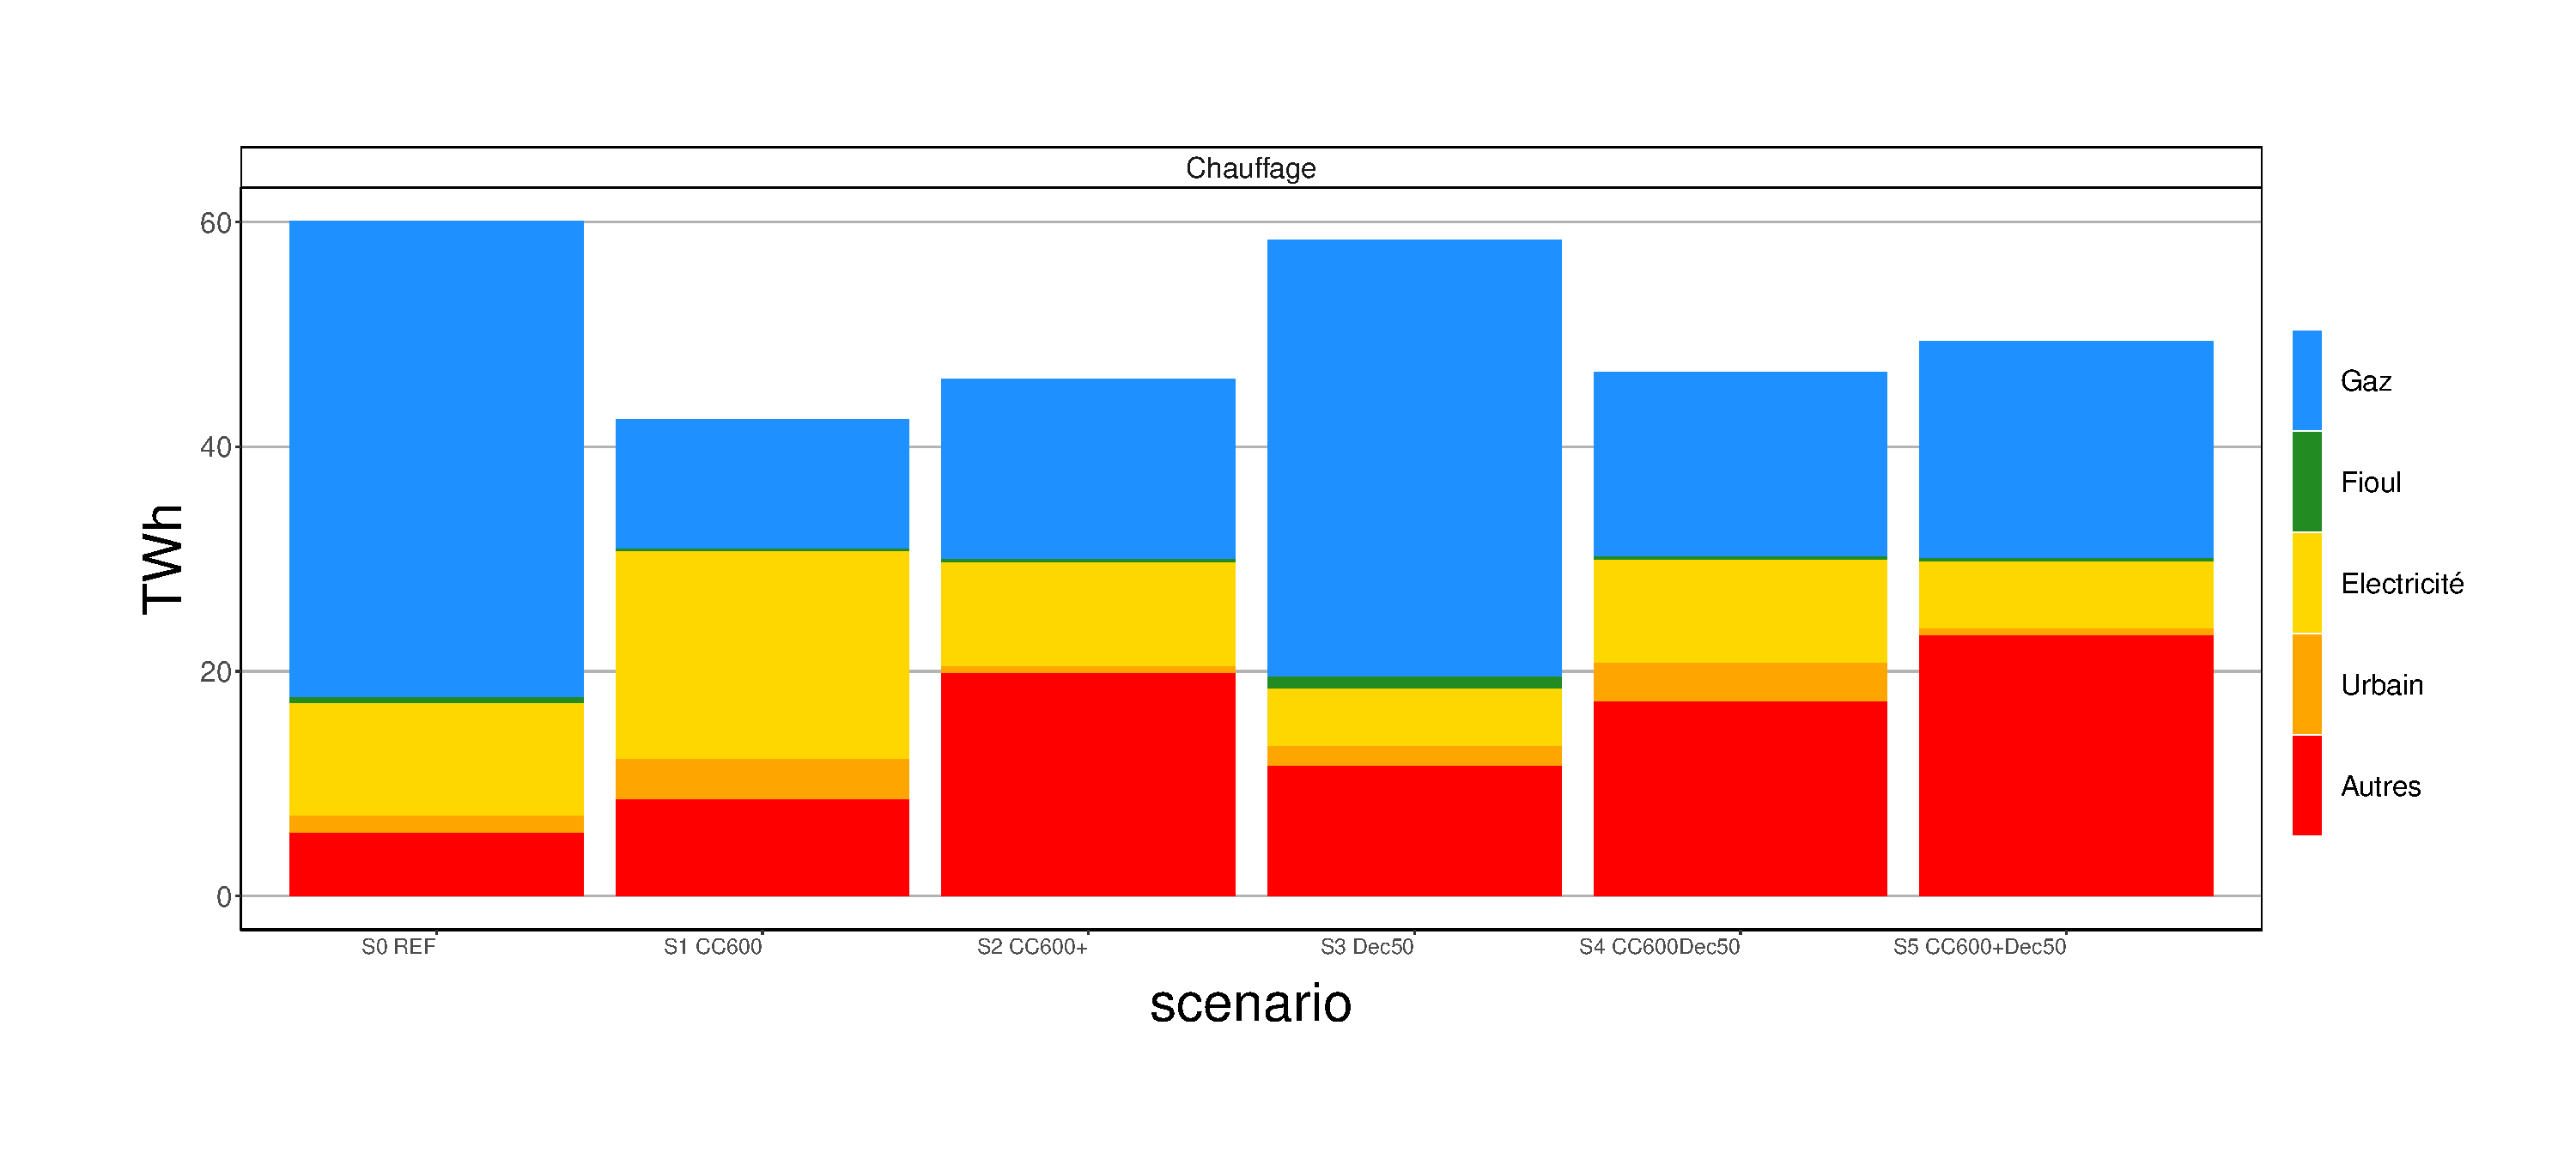
\includegraphics[width = 0.9\textwidth]{comp_cible_AMS_energie_chauffage-CC}  
\end{figure}

\begin{figure}[h!]
\centering 
\caption{Emissions de CO$_2$ liées au chauffage en 2050 par simulation}\label{Em_chauffage_2050-CC}  
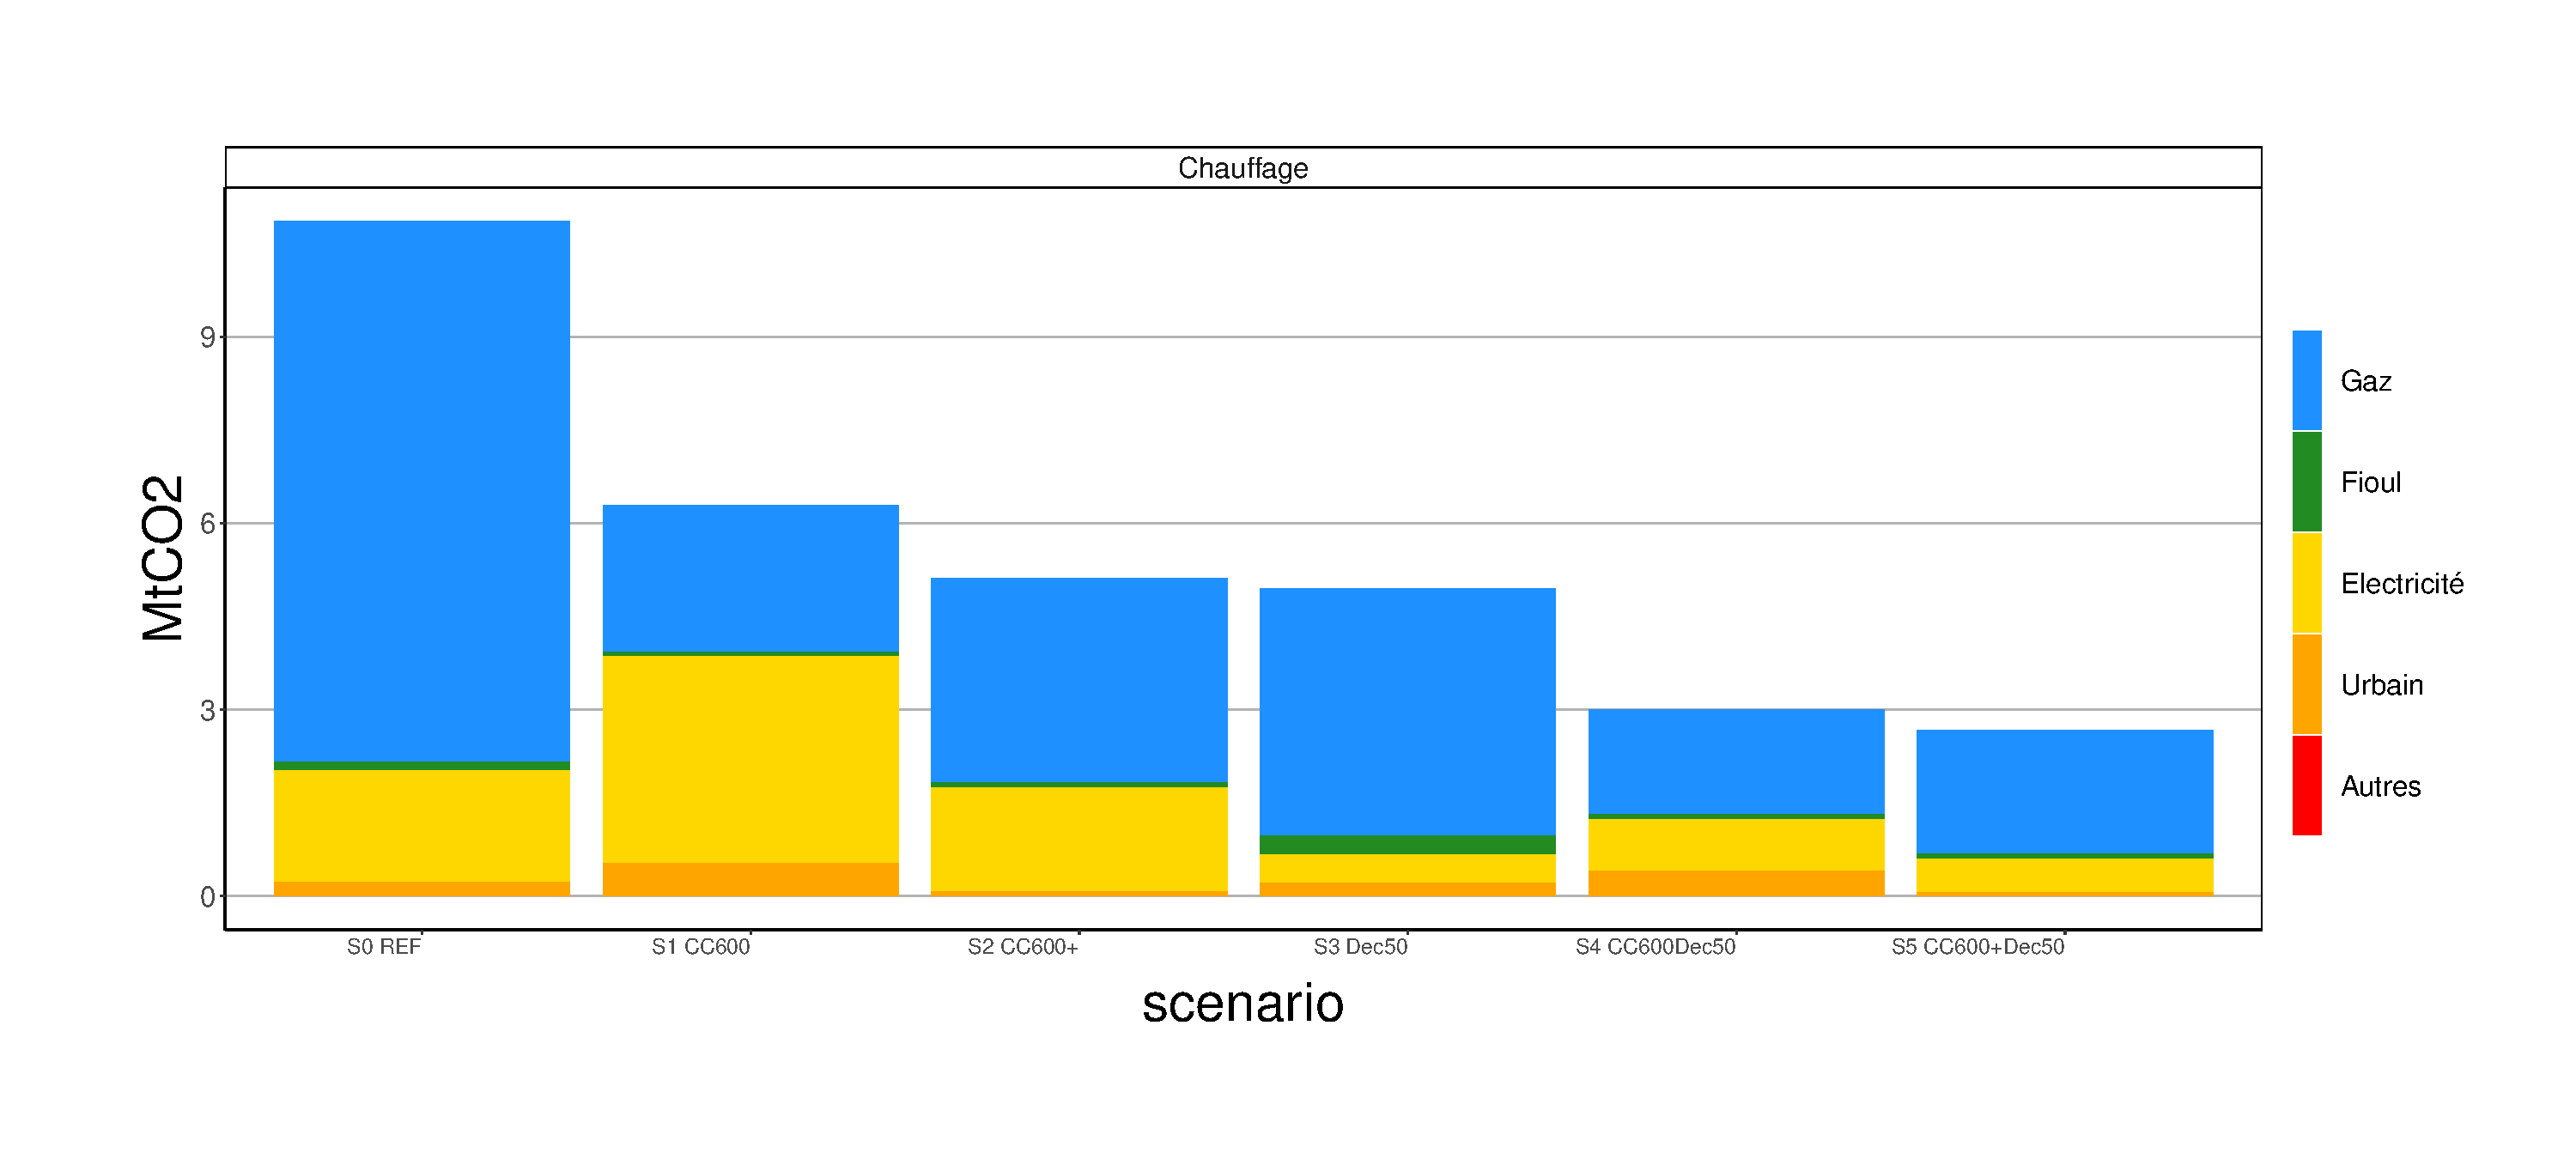
\includegraphics[width = 0.9\textwidth]{Em_chauffage_2050-CC}  
\end{figure}


\clearpage

\subsubsection{Impacts sur le budget de l’État, les usagers et analyse socio-économique}

De manière attendue, les recettes de la composante carbone croissent de 11,2 milliards d'euros (cumulées et actualisées) lorsque l'on étend son assiette à l'ensemble des énergies (scénario  \og~CC600+~\fg~) en comparaison avec le scénario \og~CC600~\fg~ où elle ne s'applique qu'au gaz et au fioul. Les recettes totales pour l’État augmente de 11 milliards d'euros ce qui représente plus que la hausse de recettes de la composante carbone car les autres recettes fiscales augmentent légèrement du fait de la moindre baisse des consommations lorsque la composante carbone s'applique à l'ensemble des énergies. Les recettes de la composante carbone sont moins élevées dans les scénarios où le mix énergétique est partiellement décarboné mais les recettes totales sont proches car les subventions sur le prix de l'électricité sont moins élevées (les usagers payent le coût complet de l'électricité, y compris la majoration de la CSPE).

\begin{table}[h] \caption{Bilan des variantes pour le budget de l’État entre 2015 et 2060}\label{Bilan_Etat_CC}
\begin{center}
\begin{tabular}[c]{|l|c|c|c|c|c|c|}
\hline
								&Recettes CC & Autres recettes fiscales & Total \\
								& 					 & (taxes - subventions) & \\
								&		(G\euro) & (G\euro) 					& (G\euro)	 \\			
\hline
REF 				&9.0 			 &3.9 	&13 \\
CC600 			& 28.6 		 &2.0 	&32 \\
CC600+ 			&39.8 		 &3.2 	&43 \\
Dec50 			&8.1			 &8.2 	&16 \\
CC600Dec50 	&25.8			 &7.6 	&33 \\
CC600+Dec50	&32.0			 &7.5 	&39 \\
\hline
\end{tabular}
\end{center}
\footnotesize{Note de lecture : Les grandeurs sont cumulées entre 2015 et 2060 et actualisées au taux public de 4,5~\%.  Les autres recettes fiscales incluent les taxes sur les énergies (hors composante carbone), les subventions éventuelles liées à la décarbonation du mix énergétique (Scénarios AMS2) et la composante énergie entre 2040 et 2050 (scénarios AMS1 et AMSDec0). On considère que les recettes des taxes et les subventions sur le prix des énergies pour l'année 2050 sont prolongées pendant 10 ans jusque 2060. Les subventions correspondant aux prêts bonifiés sont calculées comme la différence entre les annuités payées sur 10 ans pour un prêt bancaire classique avec un taux d'intérêt de 3~\% et celles payées sur 10 ans pour un prêts bonifiés avec un taux d'intérêt de 1~\%.}
\end{table}


\begin{figure}[h!]
\centering 
\caption{Recettes de la composante carbone dans les différentes variantes}\label{Evol_Recettes_CC-1}  
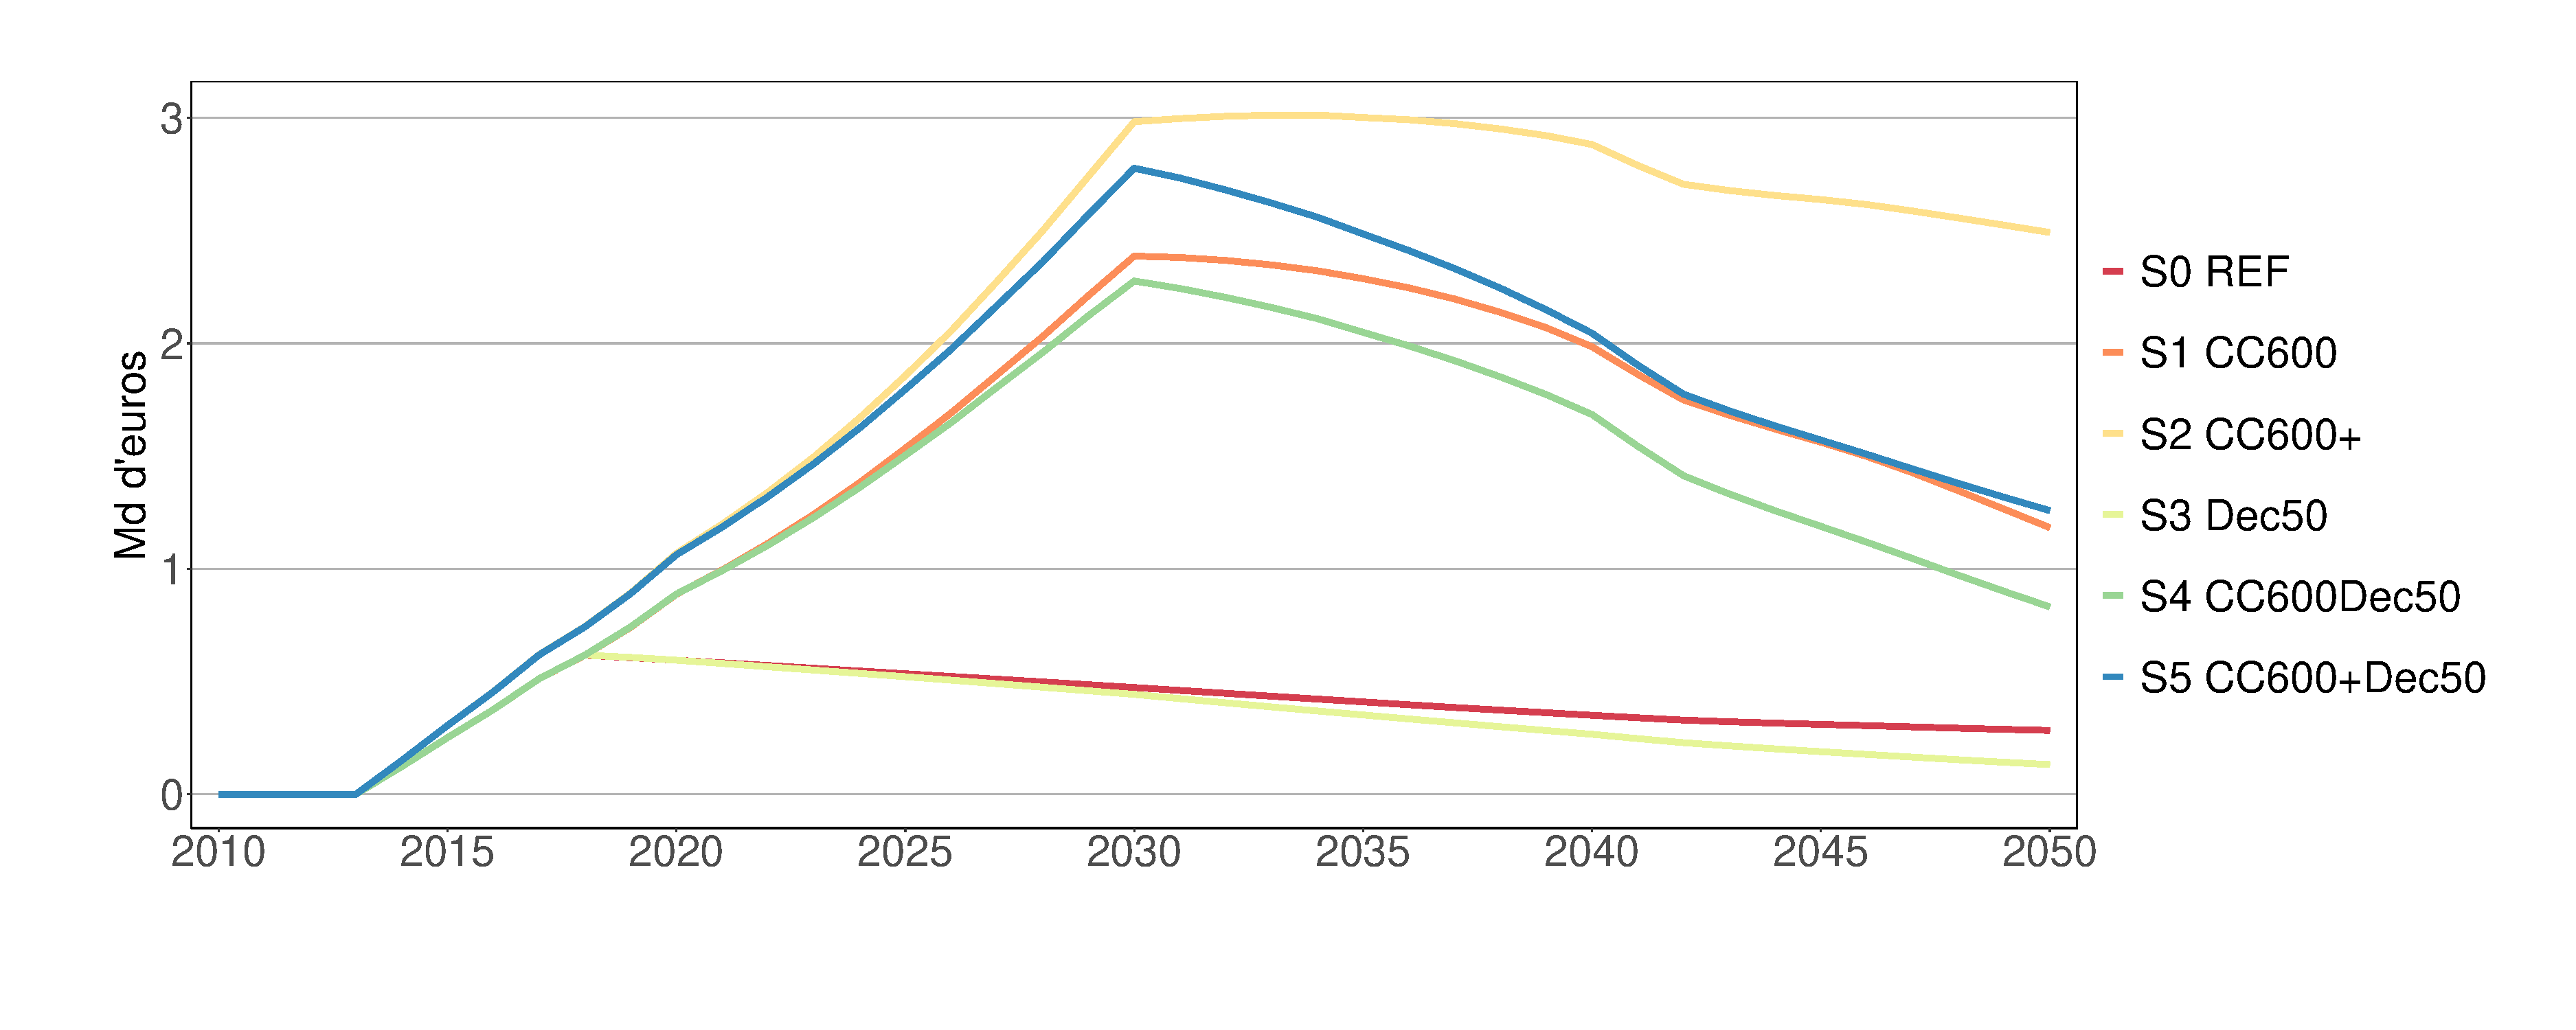
\includegraphics[width = 0.9\textwidth]{Evol_Recettes_CC-1}  
\end{figure}

%
\begin{longtable}[]{@{}crrr@{}}
\caption{bilan pour l'Etat}\tabularnewline
\toprule
\begin{minipage}[b]{0.26\columnwidth}\centering\strut
~\strut
\end{minipage} & \begin{minipage}[b]{0.17\columnwidth}\raggedleft\strut
Recettes CC\strut
\end{minipage} & \begin{minipage}[b]{0.30\columnwidth}\raggedleft\strut
Recettes autres taxes\strut
\end{minipage} & \begin{minipage}[b]{0.09\columnwidth}\raggedleft\strut
Total\strut
\end{minipage}\tabularnewline
\midrule
\endfirsthead
\toprule
\begin{minipage}[b]{0.26\columnwidth}\centering\strut
~\strut
\end{minipage} & \begin{minipage}[b]{0.17\columnwidth}\raggedleft\strut
Recettes CC\strut
\end{minipage} & \begin{minipage}[b]{0.30\columnwidth}\raggedleft\strut
Recettes autres taxes\strut
\end{minipage} & \begin{minipage}[b]{0.09\columnwidth}\raggedleft\strut
Total\strut
\end{minipage}\tabularnewline
\midrule
\endhead
\begin{minipage}[t]{0.26\columnwidth}\centering\strut
\textbf{S0 REF}\strut
\end{minipage} & \begin{minipage}[t]{0.17\columnwidth}\raggedleft\strut
9.1\strut
\end{minipage} & \begin{minipage}[t]{0.30\columnwidth}\raggedleft\strut
6.5\strut
\end{minipage} & \begin{minipage}[t]{0.09\columnwidth}\raggedleft\strut
16\strut
\end{minipage}\tabularnewline
\begin{minipage}[t]{0.26\columnwidth}\centering\strut
\textbf{S1 CC600}\strut
\end{minipage} & \begin{minipage}[t]{0.17\columnwidth}\raggedleft\strut
28.7\strut
\end{minipage} & \begin{minipage}[t]{0.30\columnwidth}\raggedleft\strut
4.7\strut
\end{minipage} & \begin{minipage}[t]{0.09\columnwidth}\raggedleft\strut
33\strut
\end{minipage}\tabularnewline
\begin{minipage}[t]{0.26\columnwidth}\centering\strut
\textbf{S2 CC600+}\strut
\end{minipage} & \begin{minipage}[t]{0.17\columnwidth}\raggedleft\strut
40.0\strut
\end{minipage} & \begin{minipage}[t]{0.30\columnwidth}\raggedleft\strut
5.9\strut
\end{minipage} & \begin{minipage}[t]{0.09\columnwidth}\raggedleft\strut
46\strut
\end{minipage}\tabularnewline
\begin{minipage}[t]{0.26\columnwidth}\centering\strut
\textbf{S3 Dec50}\strut
\end{minipage} & \begin{minipage}[t]{0.17\columnwidth}\raggedleft\strut
8.2\strut
\end{minipage} & \begin{minipage}[t]{0.30\columnwidth}\raggedleft\strut
11.0\strut
\end{minipage} & \begin{minipage}[t]{0.09\columnwidth}\raggedleft\strut
19\strut
\end{minipage}\tabularnewline
\begin{minipage}[t]{0.26\columnwidth}\centering\strut
\textbf{S4 CC600Dec50}\strut
\end{minipage} & \begin{minipage}[t]{0.17\columnwidth}\raggedleft\strut
25.9\strut
\end{minipage} & \begin{minipage}[t]{0.30\columnwidth}\raggedleft\strut
10.5\strut
\end{minipage} & \begin{minipage}[t]{0.09\columnwidth}\raggedleft\strut
36\strut
\end{minipage}\tabularnewline
\begin{minipage}[t]{0.26\columnwidth}\centering\strut
\textbf{S5 CC600+Dec50}\strut
\end{minipage} & \begin{minipage}[t]{0.17\columnwidth}\raggedleft\strut
32.1\strut
\end{minipage} & \begin{minipage}[t]{0.30\columnwidth}\raggedleft\strut
10.3\strut
\end{minipage} & \begin{minipage}[t]{0.09\columnwidth}\raggedleft\strut
42\strut
\end{minipage}\tabularnewline
\bottomrule
\end{longtable}

La composante carbone entraîne un surcoût de 24 milliards d'euros pour les usagers par rapport à un scénario sans mesures, 35 milliards d'euros si l'ensemble des énergies sont taxées (tableau \ref{Bilan_usager_CC}). Elle incite néanmoins les usagers à réaliser des investissements rentables car le surcoût aurait été de 46 milliards d'euros (respectivement 58 milliards d'euros) sans investir c'est à dire avec les consommations d'énergie du scénario sans mesures. Le surcoût est donc réduit de 22 milliards d'euros pour des investissements de 8 milliards d'euros (respectivement 10 milliards d'euros).
	
	\begin{table}[h] \caption{Coût total par scénario entre 2015 et 2060 pour les usagers des bâtiments}\label{Bilan_usager_CC}
\begin{center}
\scriptsize
\begin{tabular}[c]{|l|c|c|c|c|c|c|}
\hline
					& Investissements &  Consommations 		&	Facture  		 & Coût total & Facture 		& Coût total  \\
					&									& 	de chauffage		& énergétique & 	 usager		& (Conso REF)	&	(Conso REF) \\
					&		(G\euro)		&			(TWh)				&		(G\euro) 					& (G\euro)	 	& (G\euro) 					& (G\euro) \\
					&    (1) 				&      (2)        &      (3)            & (1)+(3) = (4) &  (5) & (1)+(5) = (6) \\
\hline
REF 					&	25 &1,601 &128 &153 & Référence & Référence\\
CC600 				&	33 &1,462 &144 &177 &166 &199 \\
CC600+ 				&	35 &1,491 &153 &188 &176 &211 \\
Dec50 				&	28 &1,602 &139 &166 &143 &171 \\
CC600Dec50 		&	35 &1,490 &151 &185 &171 &206 \\
CC600+Dec50		&	36 &1,513 &155 &191 &178 &214 \\
\hline
\end{tabular}
\end{center}
	\footnotesize{Note de lecture : Les grandeurs sont cumulées entre 2015 et 2060 et actualisées au taux public de 4,5~\%.  La facture énergétique est calculée en multipliant les consommations aux prix des énergies HTVA mais incluant l'ensemble des taxes sur les énergies (y compris la composante carbone et la composante énergie)  On considère que les consommations pour l'année 2050 sont prolongées pendant 10 ans jusque 2060. Les investissements incluent la partie financées par les CEE}
\end{table}

Le coût d'abattement de la composante carbone seule appliquée au gaz et au fioul seulement est faible autour de 13\euro/tCO$_2$ (\ref{Bilan_socio__CC}). Le coût d'abattement diminue lorsqu'on étend la composante carbone aux autres énergies, l'efficience la mesure augmente lorsque son assiette est plus large. Le coût d'abattement de la décarbonation du mix énergétique à 50~\% est presque 6 fois plus élevé : 75~\euro/tCO$_2$ pour le scénario  \og~Dec50~\fg. La combinaison de la décarbonation et de la composante carbone permet de réduire le coût par tonne de CO$_2$ évitée et d'atteindre les réductions d'émissions cumulées les plus importantes. 
	
\begin{table}[h] \caption{Analyse socio-économique entre 2015 et 2060, scénario de référence  = AME}\label{Bilan_socio__CC} 
\begin{center}
\scriptsize
\begin{tabular}[c]{|l|c|c|c|c|c|c|c|c|}
\hline
			& Investissements	& Facture HT & Emissions	& Coût total  &	Coût 						& COFP	&Coût total	& Coût 					 \\
			&									&						 & 						&							&	d'abattement		&				&avec COFP	& d'abattement 	 \\	
			&									&						 &						&							&					&				&						&	avec COFP 				\\
			&		(G\euro)			&		(G\euro) &	(MtCO$_2$)&	(G\euro)		&	(\euro/tCO$_2$)	&	(G\euro) & (G\euro) & 	(\euro/tCO$_2$)	 \\
			&   (1) 					&    (2) 		 &   (3) 			&  (1) + (2) = (4)  &  		(5)			& 	(6)		&    (4)+(6)=(7)       &      $C_{CO_2}$= (8)          \\
\hline
REF 				&25 &115 &600 &140 &Référence &-3.2	&137 &Référence \\
CC600 			&33 &113 &490 &146 &53 &-7.7 				&138 &13	\\
CC600+ 			&35 &110 &470 &145 &36 &-10.8 			&134 &-22\\
Dec50 			&28 &122 &477 &150 &81 &-4.1 				&146 &74\\
CC600Dec50 	&35 &117 &411 &152 &62 &-8.4 				&144 &35\\
CC600+Dec50 &36 &116 &407 &152 &59 &-9.9 				&142 &24\\
\hline
\end{tabular}
\end{center}
\footnotesize{Note de lecture : Les investissements, la facture énergétique hors taxes  et le COFP sont cumulés entre 2015 et 2060 et actualisées au taux public de 4,5~\%.  La facture énergétique est calculée en multipliant les consommations aux prix des énergies HTVA  sans inclure l'ensemble des taxes sur les énergies et les subventions liées à la décarbonation des énergies. On considère que les consommations pour l'année 2050 sont prolongées pendant 10 ans jusque 2060. Ce prix représente le \og~vrai coût~\fg de production des énergies. Les investissements incluent la partie financées par les CEE. Le COFP est calculé comme étant égal à 25~\% des recettes fiscales des taxes sur les énergies moins les subventions à la décarbonation du mix énergétique, moins les subventions correspondant aux prêts bonifiés. On considère que les recettes des taxes et les subventions sur le prix des énergies pour l'année 2050 sont prolongées pendant 10 ans jusque 2060.}

\end{table}

	%\begin{longtable}[]{@{}crrrrrrrr@{}}
\caption{bilan pour la société}\tabularnewline
\toprule
\begin{minipage}[b]{0.10\columnwidth}\centering\strut
~\strut
\end{minipage} & \begin{minipage}[b]{0.09\columnwidth}\raggedleft\strut
Investissements\strut
\end{minipage} & \begin{minipage}[b]{0.06\columnwidth}\raggedleft\strut
Facture HT\strut
\end{minipage} & \begin{minipage}[b]{0.06\columnwidth}\raggedleft\strut
Emissions\strut
\end{minipage} & \begin{minipage}[b]{0.07\columnwidth}\raggedleft\strut
Coût total\strut
\end{minipage} & \begin{minipage}[b]{0.07\columnwidth}\raggedleft\strut
Coût tonne\strut
\end{minipage} & \begin{minipage}[b]{0.04\columnwidth}\raggedleft\strut
COFP\strut
\end{minipage} & \begin{minipage}[b]{0.13\columnwidth}\raggedleft\strut
Coût total avec COFP\strut
\end{minipage} & \begin{minipage}[b]{0.13\columnwidth}\raggedleft\strut
Coût tonne avec COFP\strut
\end{minipage}\tabularnewline
\midrule
\endfirsthead
\toprule
\begin{minipage}[b]{0.10\columnwidth}\centering\strut
~\strut
\end{minipage} & \begin{minipage}[b]{0.09\columnwidth}\raggedleft\strut
Investissements\strut
\end{minipage} & \begin{minipage}[b]{0.06\columnwidth}\raggedleft\strut
Facture HT\strut
\end{minipage} & \begin{minipage}[b]{0.06\columnwidth}\raggedleft\strut
Emissions\strut
\end{minipage} & \begin{minipage}[b]{0.07\columnwidth}\raggedleft\strut
Coût total\strut
\end{minipage} & \begin{minipage}[b]{0.07\columnwidth}\raggedleft\strut
Coût tonne\strut
\end{minipage} & \begin{minipage}[b]{0.04\columnwidth}\raggedleft\strut
COFP\strut
\end{minipage} & \begin{minipage}[b]{0.13\columnwidth}\raggedleft\strut
Coût total avec COFP\strut
\end{minipage} & \begin{minipage}[b]{0.13\columnwidth}\raggedleft\strut
Coût tonne avec COFP\strut
\end{minipage}\tabularnewline
\midrule
\endhead
\begin{minipage}[t]{0.10\columnwidth}\centering\strut
\textbf{S0 REF}\strut
\end{minipage} & \begin{minipage}[t]{0.09\columnwidth}\raggedleft\strut
31\strut
\end{minipage} & \begin{minipage}[t]{0.06\columnwidth}\raggedleft\strut
154\strut
\end{minipage} & \begin{minipage}[t]{0.06\columnwidth}\raggedleft\strut
710\strut
\end{minipage} & \begin{minipage}[t]{0.07\columnwidth}\raggedleft\strut
185\strut
\end{minipage} & \begin{minipage}[t]{0.07\columnwidth}\raggedleft\strut
NA\strut
\end{minipage} & \begin{minipage}[t]{0.04\columnwidth}\raggedleft\strut
-3.9\strut
\end{minipage} & \begin{minipage}[t]{0.13\columnwidth}\raggedleft\strut
181\strut
\end{minipage} & \begin{minipage}[t]{0.13\columnwidth}\raggedleft\strut
NA\strut
\end{minipage}\tabularnewline
\begin{minipage}[t]{0.10\columnwidth}\centering\strut
\textbf{S1 CC600}\strut
\end{minipage} & \begin{minipage}[t]{0.09\columnwidth}\raggedleft\strut
39\strut
\end{minipage} & \begin{minipage}[t]{0.06\columnwidth}\raggedleft\strut
152\strut
\end{minipage} & \begin{minipage}[t]{0.06\columnwidth}\raggedleft\strut
600\strut
\end{minipage} & \begin{minipage}[t]{0.07\columnwidth}\raggedleft\strut
191\strut
\end{minipage} & \begin{minipage}[t]{0.07\columnwidth}\raggedleft\strut
53\strut
\end{minipage} & \begin{minipage}[t]{0.04\columnwidth}\raggedleft\strut
-8.3\strut
\end{minipage} & \begin{minipage}[t]{0.13\columnwidth}\raggedleft\strut
183\strut
\end{minipage} & \begin{minipage}[t]{0.13\columnwidth}\raggedleft\strut
13\strut
\end{minipage}\tabularnewline
\begin{minipage}[t]{0.10\columnwidth}\centering\strut
\textbf{S2 CC600+}\strut
\end{minipage} & \begin{minipage}[t]{0.09\columnwidth}\raggedleft\strut
42\strut
\end{minipage} & \begin{minipage}[t]{0.06\columnwidth}\raggedleft\strut
148\strut
\end{minipage} & \begin{minipage}[t]{0.06\columnwidth}\raggedleft\strut
580\strut
\end{minipage} & \begin{minipage}[t]{0.07\columnwidth}\raggedleft\strut
190\strut
\end{minipage} & \begin{minipage}[t]{0.07\columnwidth}\raggedleft\strut
36\strut
\end{minipage} & \begin{minipage}[t]{0.04\columnwidth}\raggedleft\strut
-11.5\strut
\end{minipage} & \begin{minipage}[t]{0.13\columnwidth}\raggedleft\strut
178\strut
\end{minipage} & \begin{minipage}[t]{0.13\columnwidth}\raggedleft\strut
-22\strut
\end{minipage}\tabularnewline
\begin{minipage}[t]{0.10\columnwidth}\centering\strut
\textbf{S3 Dec50}\strut
\end{minipage} & \begin{minipage}[t]{0.09\columnwidth}\raggedleft\strut
34\strut
\end{minipage} & \begin{minipage}[t]{0.06\columnwidth}\raggedleft\strut
161\strut
\end{minipage} & \begin{minipage}[t]{0.06\columnwidth}\raggedleft\strut
588\strut
\end{minipage} & \begin{minipage}[t]{0.07\columnwidth}\raggedleft\strut
195\strut
\end{minipage} & \begin{minipage}[t]{0.07\columnwidth}\raggedleft\strut
82\strut
\end{minipage} & \begin{minipage}[t]{0.04\columnwidth}\raggedleft\strut
-4.8\strut
\end{minipage} & \begin{minipage}[t]{0.13\columnwidth}\raggedleft\strut
190\strut
\end{minipage} & \begin{minipage}[t]{0.13\columnwidth}\raggedleft\strut
75\strut
\end{minipage}\tabularnewline
\begin{minipage}[t]{0.10\columnwidth}\centering\strut
\textbf{S4 CC600Dec50}\strut
\end{minipage} & \begin{minipage}[t]{0.09\columnwidth}\raggedleft\strut
41\strut
\end{minipage} & \begin{minipage}[t]{0.06\columnwidth}\raggedleft\strut
156\strut
\end{minipage} & \begin{minipage}[t]{0.06\columnwidth}\raggedleft\strut
522\strut
\end{minipage} & \begin{minipage}[t]{0.07\columnwidth}\raggedleft\strut
197\strut
\end{minipage} & \begin{minipage}[t]{0.07\columnwidth}\raggedleft\strut
63\strut
\end{minipage} & \begin{minipage}[t]{0.04\columnwidth}\raggedleft\strut
-9.1\strut
\end{minipage} & \begin{minipage}[t]{0.13\columnwidth}\raggedleft\strut
188\strut
\end{minipage} & \begin{minipage}[t]{0.13\columnwidth}\raggedleft\strut
35\strut
\end{minipage}\tabularnewline
\begin{minipage}[t]{0.10\columnwidth}\centering\strut
\textbf{S5 CC600+Dec50}\strut
\end{minipage} & \begin{minipage}[t]{0.09\columnwidth}\raggedleft\strut
42\strut
\end{minipage} & \begin{minipage}[t]{0.06\columnwidth}\raggedleft\strut
154\strut
\end{minipage} & \begin{minipage}[t]{0.06\columnwidth}\raggedleft\strut
518\strut
\end{minipage} & \begin{minipage}[t]{0.07\columnwidth}\raggedleft\strut
197\strut
\end{minipage} & \begin{minipage}[t]{0.07\columnwidth}\raggedleft\strut
59\strut
\end{minipage} & \begin{minipage}[t]{0.04\columnwidth}\raggedleft\strut
-10.6\strut
\end{minipage} & \begin{minipage}[t]{0.13\columnwidth}\raggedleft\strut
186\strut
\end{minipage} & \begin{minipage}[t]{0.13\columnwidth}\raggedleft\strut
24\strut
\end{minipage}\tabularnewline
\bottomrule
\end{longtable}

\clearpage
\newpage 

\subsection{Décarbonation}

Des calculs complémentaires pour estimer un coût d’abattement en distinguant deux effets :  
\begin{itemize}
	\item Effet « changement de mix sans rénovation » ≈  XX euros par tonne évitée
	\item Effet « rénovation sans changement de mix »  ≈  XX euros par tonne évitée 
\end{itemize}


\subsection{Comparaison aux autres mesures sur la rénovation énergétique}

\subsubsection{Scénarios comparés}

Pour comparer l'impact unitaire de la composante carbone à celui des autres mesures sur la rénovation énergétique, nous comparons ici 6 simulations du modèle :

\begin{itemize}
	\item Les scénarios \og~REF~\fg, \og~CC600~\fg~, \og~CC600+~\fg~ \og~CC600+~\fg~ et \og~Dec50~\fg~ précédent
	\item Le scénario \og~CEE~\fg dans lequel les CEE sont la seule mesure activée. Ils sont modélisés comme dans les scénarios AMS et maintenus jusque 2050
	\item Le scénario \og~OR~\fg dans lequel les obligations de rénovation (décret travaux embarqués, décret de rénovation du parc tertiaire et Directive européenne « Patrimoine de l’État : efficacité énergétique »). Ces obligations de rénovation sont modélisées comme dans les scénarios AMS
	
\end{itemize}


\subsubsection{Contribution des mesures à l'objectif de baisse des consommations et des émissions (efficacité)}

En 2050, la composante carbone à 600 euros par tonne de CO$_2$ permet de réduire les consommations de chauffage et les émissions de CO$_2$ liées au chauffage des bâtiments tertiaires de 17 TWh et de 4,6 MtCO$_2$ par rapport à un scénario sans aucune mesure, 14 TWh et 5,8 MtCO$_2$ lorsqu'elle s'applique à l'ensemble des énergies. Au total, cela représente respectivement 119 MtCO$_2$ et 141 MtCO$_2$ évitées entre 2015 et 2060. 

La décarbonation du mix énergétique  à 50 ~\%  a peu d'impacts sur les consommations en 2050 (-2 TWh par rapport à un scénario sans mesure du fait de la hausse des prix des énergies décarbonées pour les usagers) mais permet de réduire  les émissions 5,9 MtCO$_2$ en 2050 par rapport à un scénario sans aucune mesure (-54~\% par rapport au scénario sans mesures). En cumulé, cela 136 MtCO$_2$ évitées entre 2015 et 2060 soit une contribution du même ordre de grandeur que la composante carbone. 

L’impact des autres mesures comme les CEE ou les obligations de rénovation est moindre sur les émissions (respectivement -1,4 MtCO$_2$  et -0,8 MtCO$_2$ en 2050 par rapport à un scénario sans mesures, 35 et 19  MtCO$_2$ évitées évitées entre 2015 et 2060). Les CEE ont en revanche un impact assez important sur la baisse des consommations de chauffage (-9 TWh en 2050 par rapport au scénario sans mesures). 


\begin{figure}[h!]
\centering 
\caption{Consommations de chauffage en 2050 par simulation}\label{comp_cible_AMS_energie_chauffage-1}  
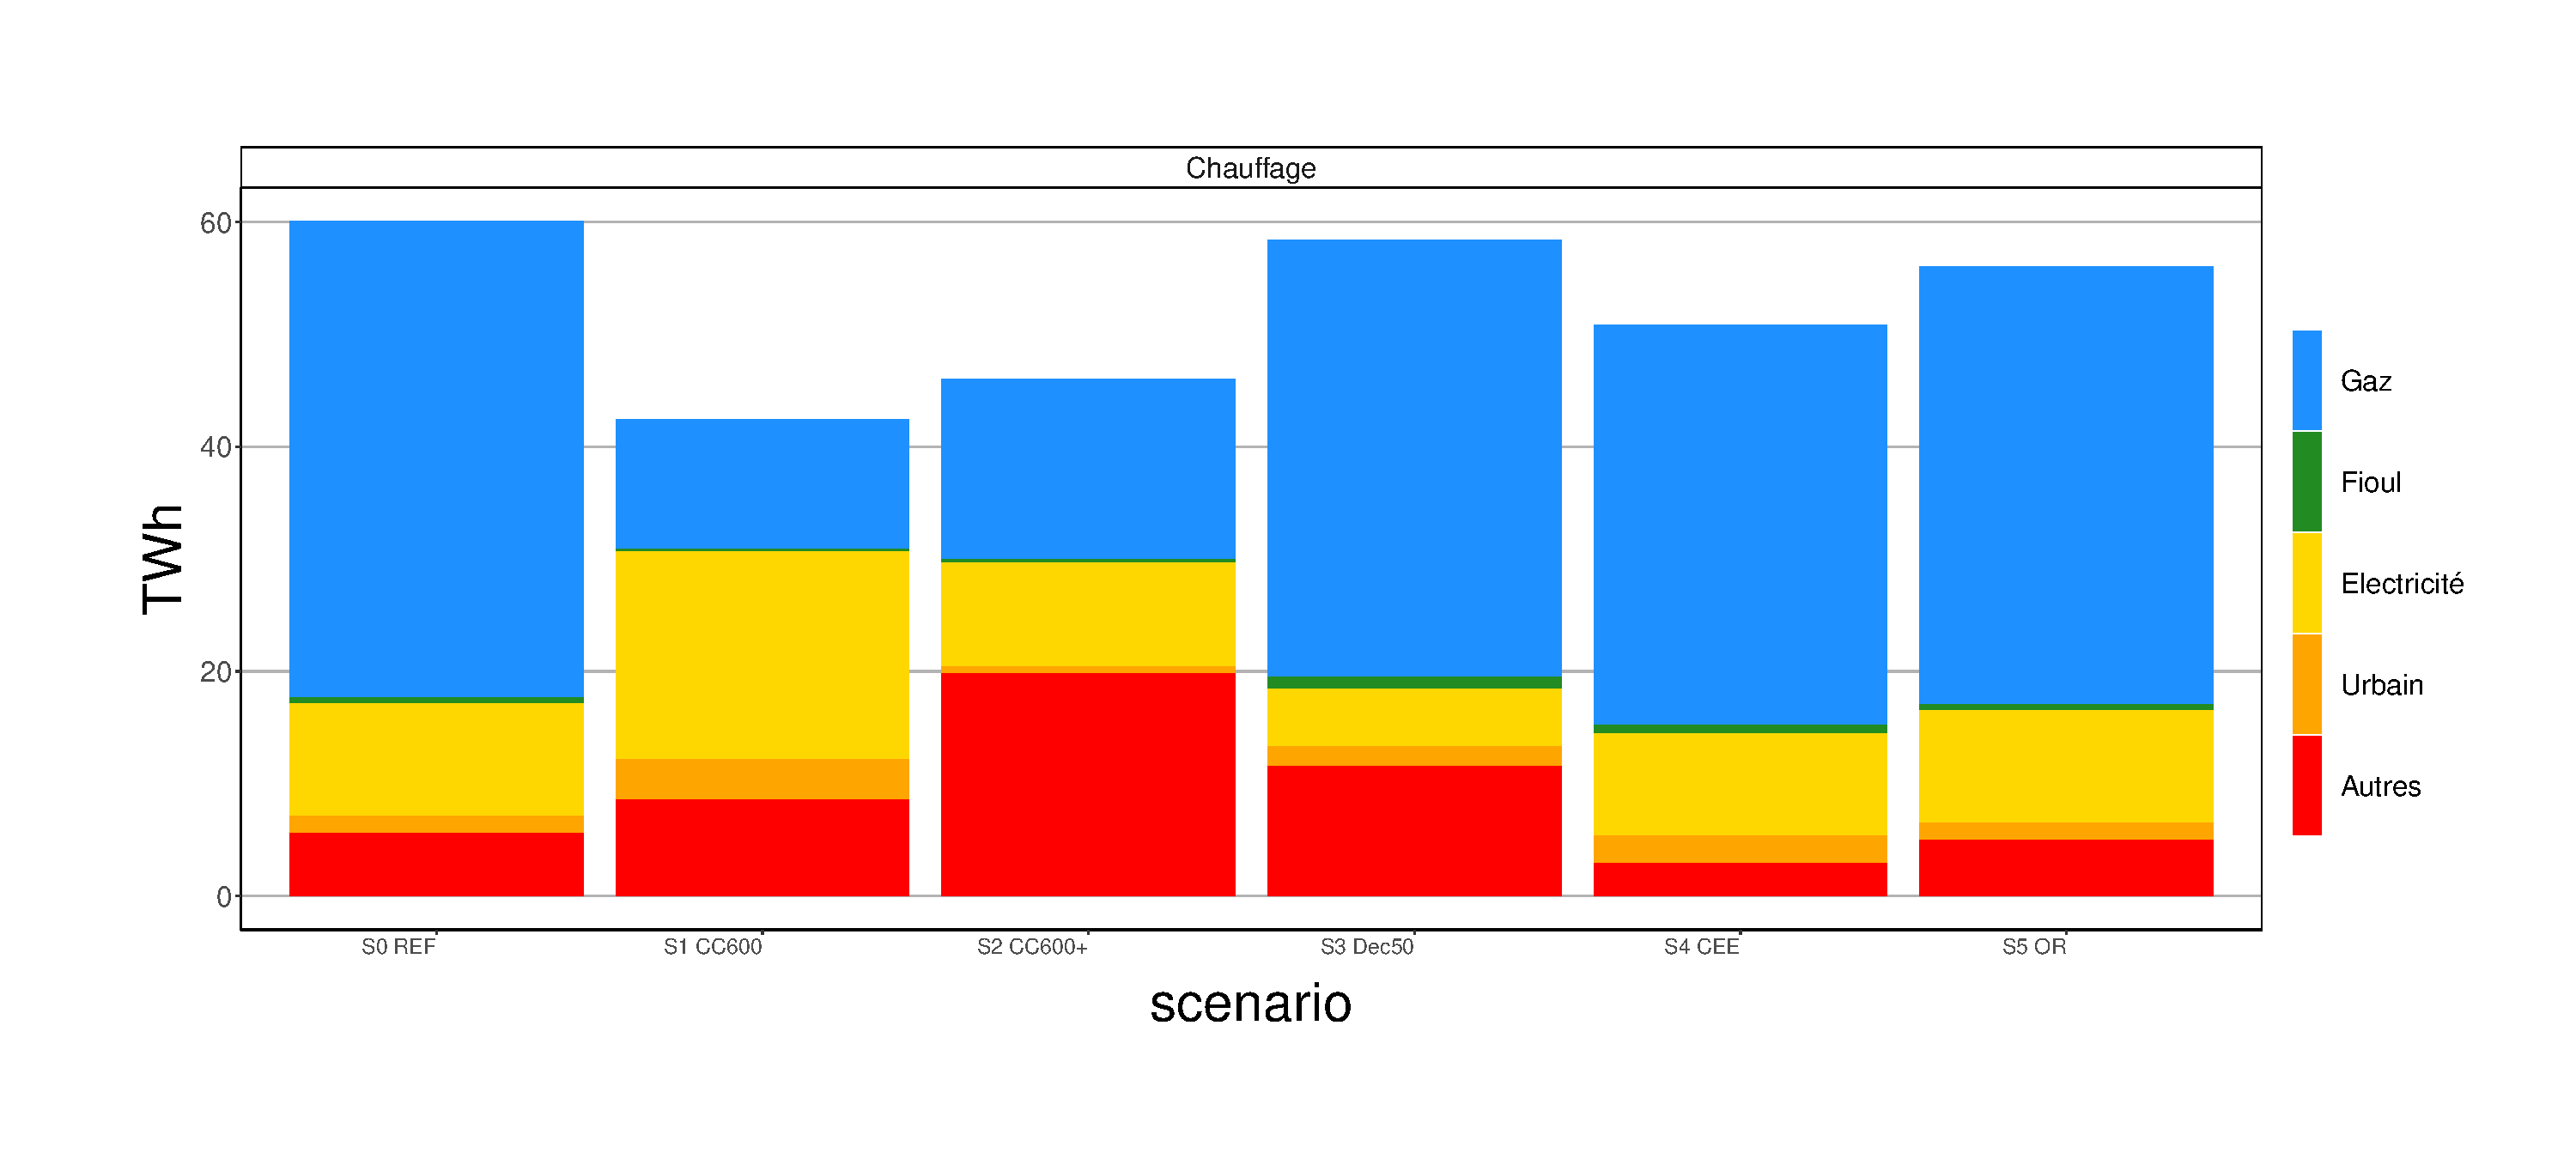
\includegraphics[width = 0.9\textwidth]{comp_cible_AMS_energie_chauffage-1}  
\end{figure}

\begin{figure}[h!]
\centering 
\caption{Emissions de CO$_2$ liées au chauffage en 2050 par simulation}\label{Em_chauffage_2050-1}  
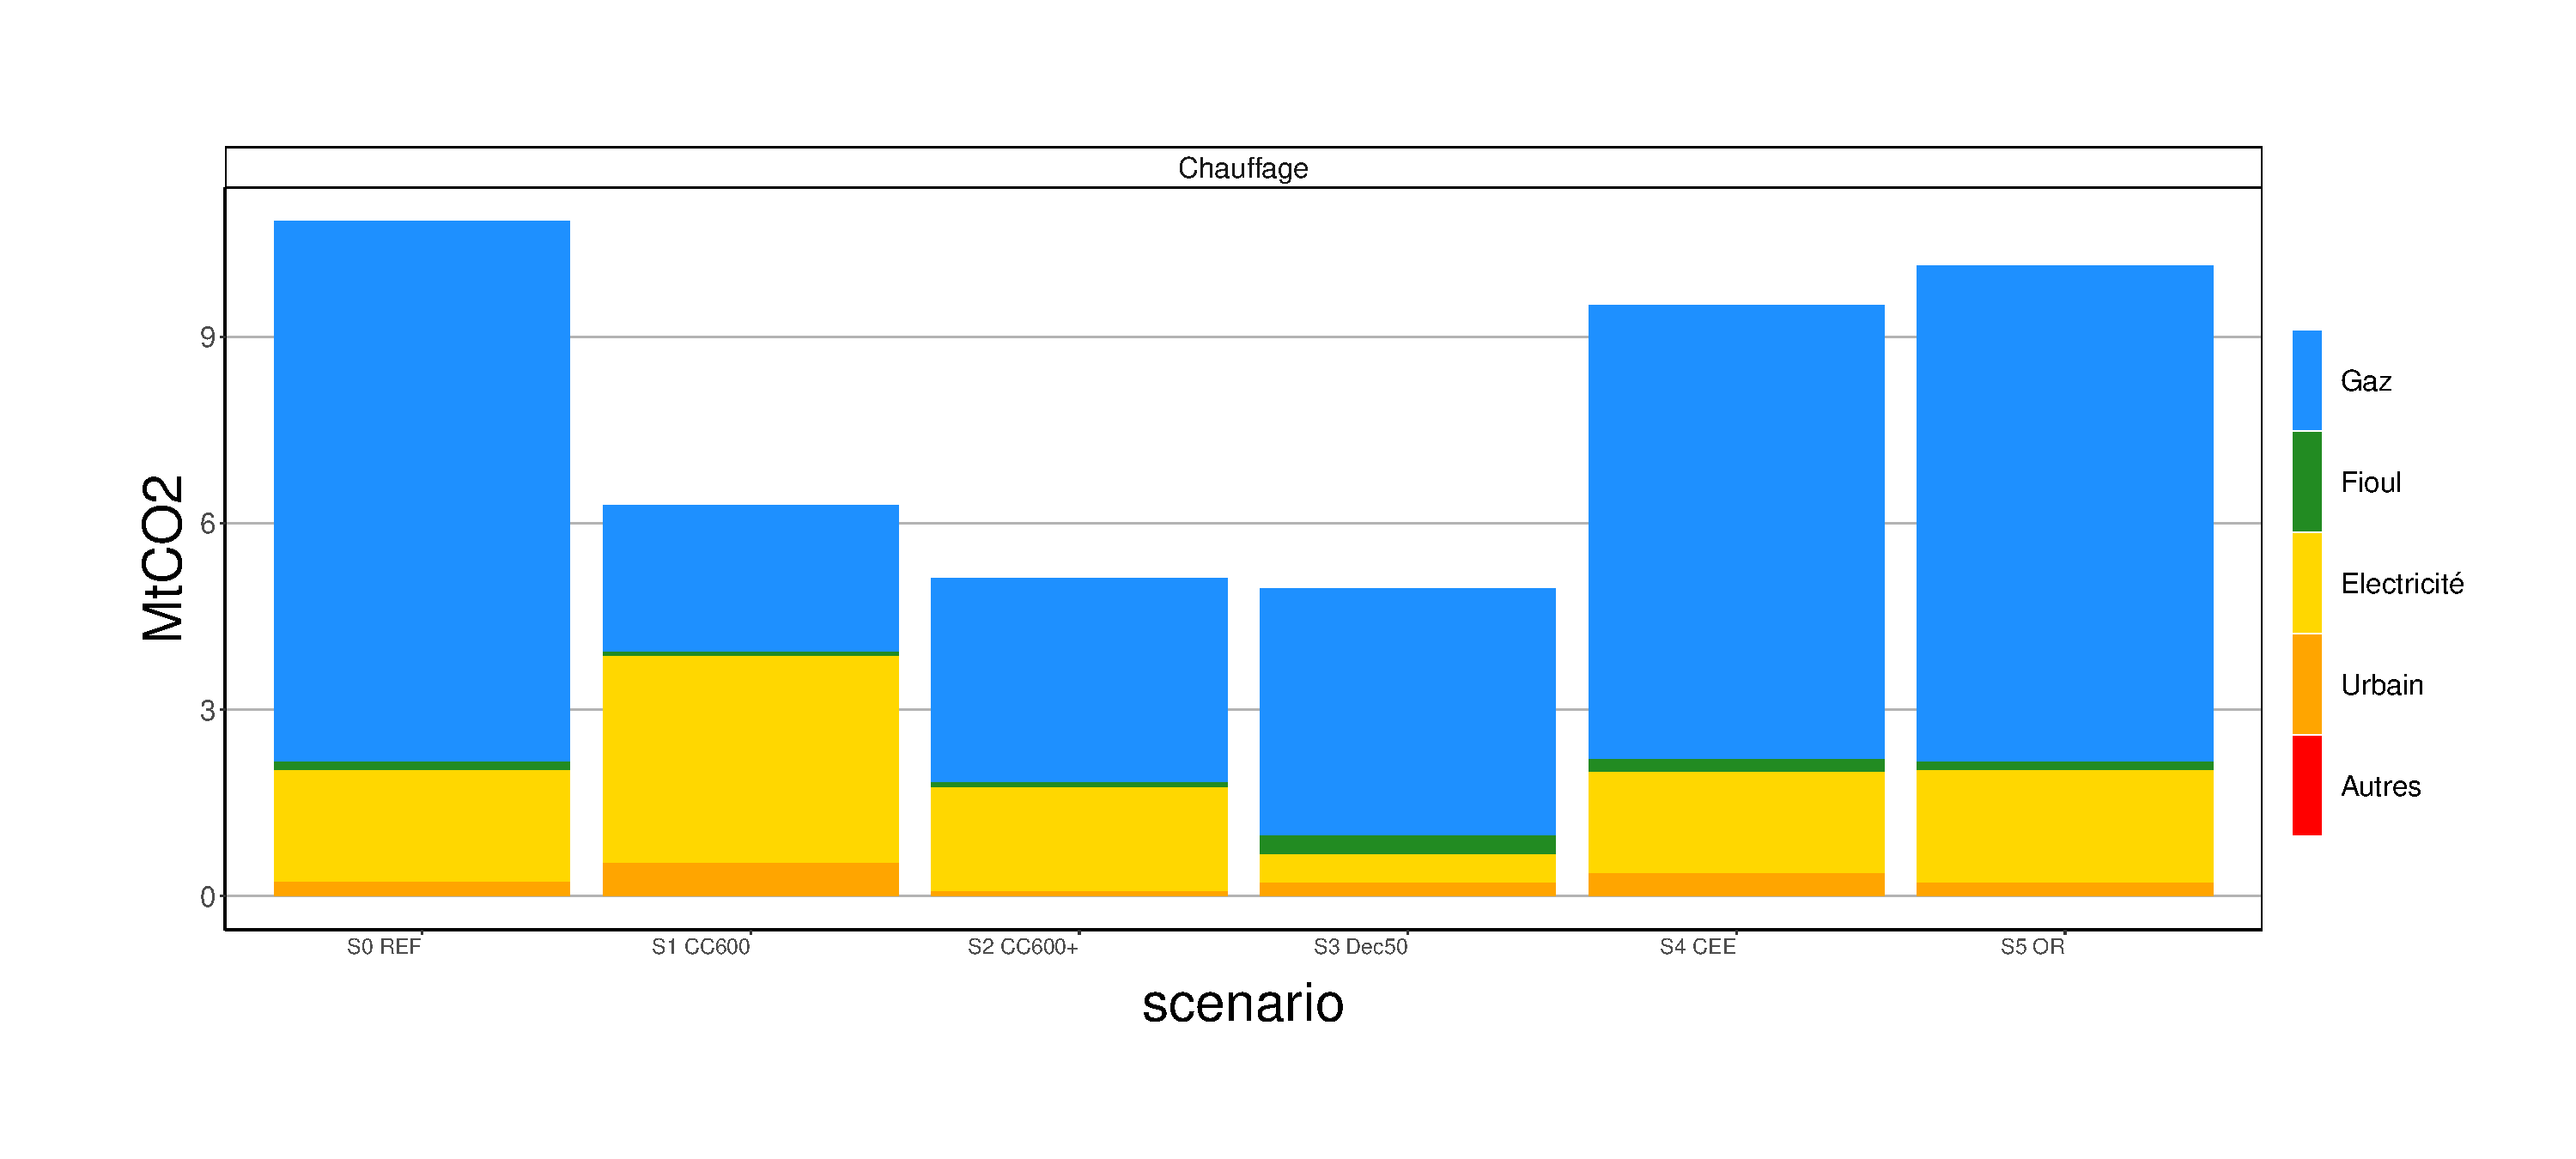
\includegraphics[width = 0.9\textwidth]{Em_chauffage_2050-1}  
\end{figure}

\subsubsection{Efficience comparée des mesures}

La figure \ref{compmesures} compare l'efficience (coût d'abattement) et l'efficacité à réduire les émissions de CO$_2$ liées au chauffage cumulées entre 2015 et 2060 pour le parc existant des différentes simulations évoquées ci-dessus ainsi que des scénarios comprenant une combinaison de mesures (AME, AMS1, AMS2, AMSDec0). Les émissions cumulées du scénario REF sans mesures (600 MtCO$_2$ pour le chauffage du parc existant entre 2015 et 2060)  sont représentées par la ligne noire verticale.

Les obligations de rénovation telles qu'elles sont modélisées dans ce scénario ont un coût d'abattement très élevé et un impact assez limité sur les émissions du parc tertiaire existant. 

Les CEE ont un coût d'abattement faible mais peu d'impact sur les émissions, l'impact principal de cette mesure étant de faire diminuer les consommations d'énergie mais pas d'orienter les 
usagers vers des énergies moins carbonées comme peut le faire la composante carbone. 

La composante carbone avec ces deux variantes et la décarbonation des énergies permettent de réduire significativement les émissions liées au chauffage. Ces mesures permettent à elles seules d'éviter plus d'émissions que l'ensemble des mesures existantes (scénario AME).Avec les hypothèses retenues sur les coûts de décarbonation de l'énergie, l'efficience de la composante carbone est supérieure à celle de la décarbonation des vecteurs. Son efficience augmente lorsque l'on étend son assiette à l'ensemble des énergies. En combinant l'ensemble des mesures (scénarios AMS1 et AMS2), il est possible de réduire drastiquement les émissions (division par presque 2 des émissions cumulées)  pour un coût d'abattement plus élevé que celui de la composante carbone seule, mais raisonnable si on le compare aux estimations réalisées dans d'autres secteurs comme le secteur des transports. 


\begin{figure}[h!]
\centering 
\caption{Coût à la tonne de CO$2$ évitée et émissions de CO$_2$ du parc existant liées au chauffage cumulées  entre 2015 et 2060 par mesure et par scénario}\label{compmesures}  
\includegraphics[width = 0.9\textwidth]{compmesures}  
\end{figure}

\cleardoublepage

\section{Conclusion}\label{sec:marker7}

\markboth{Conclusion}{}

\cleardoublepage

\thispagestyle{partie}
\cadreblanc{Partie 6}{Annexes}{}

\newpage
\pagestyle{fancy}
\invisiblesection{Annexes}\label{sec:marker8}
\markboth{Annexes}{}


\cleardoublepage

%\thispagestyle{partie}
%\cadreblanc{Partie 7}{R\'ef\'erences}{}

%\newpage
\pagestyle{fancy}
\invisiblesection{R\'ef\'erences}\label{sec:marker9}
%\section{R\'ef\'erences}\label{sec:marker8}
\markboth{R\'ef\'erences}{}

\bibliographystyle{apalike-fr}
\bibliography{biblio_tertiaire}

%\addcontentsline{toc}{section}{R\'ef\'erences}

%Pour s'assurer que le doc termine sur une page paire
\cleardoublepage

\thispagestyle{partie}
\troisieme{}{}

\newpage 

\thispagestyle{partie}
\quatrieme{A COMPLETER}
\end{document}
}
